\باب{تفرق کا استعمال}
اس باب میں ہم تفرق سے نتائج اخذ کرنا سیکھیں گے۔ ہم تفرق کی مدد سے تفاعل کی انتہائی قیمتیں حاصل کرتے ہوئے ان کی ترسیم کی اشکال کی پیش گوئی کرتے ہیں اور ان پر تجزیہ کرتے ہیں، پیچیدہ کلیات کی سادہ صورت اخذ کرتے ہیں، تفاعل کی پیمائشی خلل کو حساسیت پر غور کرتے ہیں اور تفاعل کی صفر کو اعدادی طریقوں سے حاصل کرتے ہیں۔مسئلہ اوسط قیمت ان تمام کو ممکن بناتا ہے جس کا ایک منطقی نتیجہ تکملی احصاء کی راہ ہموار کرتا ہے۔  

\حصہ{تفاعل کی انتہائی قیمتیں}\شناخت{حصہ_استعمال_تفاعل_کی_انتہائی_قیمتیں}
اس حصہ میں استمراری تفاعل کی انتہائی قیمتوں کا مقام اور اور ان کی پہچان سکھائی جائے گی۔

\جزوحصہء{مسئلہ کم سے کم اور زیادہ سے زیادہ}
بند دائرہ کار کے ہر نقطہ پر استمراری تفاعل کا اس دائرہ کار پر مطلق بلند تر قیمت اور مطلق کم سے کم قیمت ہو گا جن پر ترسیم کھینچتے وقت  نظر رکھا جاتا ہے۔ مسائل کے حل میں ان انتہائی قیمتوں  کے کردار پر اس باب میں  جبکہ تکمل احصاء کی  نظریہ مرتب کرنے میں ان کے کردار پر اگلے دو ابواب میں غور کیا جائے گا۔  

\ابتدا{مسئلہ}\شناخت{مسئلہ_استعمال_بلند_تر_کمتر}\موٹا{استمراری تفاعل کا مسئلہ کم سے کم اور زیادہ سے زیادہ}\\
بند دائرہ کار \عددی{I} کے ہر نقطہ پر استمراری تفاعل \عددی{f} کا \عددی{I} پر مطلق زیادہ سے زیادہ قیمت \عددی{M} اور مطلق کم سے کم  قیمت \عددی{m} پایا جائے گا۔یعنی \عددی{I} میں ایسا \عددی{x_1} اور \عددی{x_2} پایا جائے گا کہ \عددی{f(x_1)=m} اور \عددی{f(x_2)=M} ہوں اور \عددی{I} میں تمام \عددی{x} کے لئے \عددی{m\le f(x)\le M} ہو (شکل \حوالہ{شکل_استعمال_بلند_تر_کم_تر})۔
\انتہا{مسئلہ}
%===================
درج بالا مسئلے کے ثبوت کے لئے حقیقی اعدادی نظام کا تفصیلی علم ضروری ہے لہٰذا اس کا ثبوت پیش نہیں کیا جائے گا۔ 
\begin{figure}
\centering
\begin{subfigure}{0.5\textwidth}
\centering
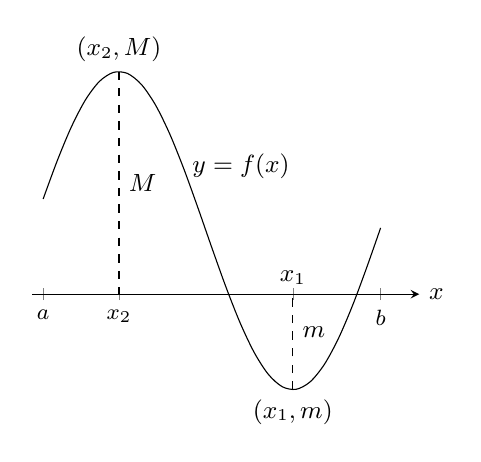
\begin{tikzpicture}[font=\small,declare function={f(\x)=0.4+sin(deg(\x));}]
\pgfmathsetmacro{\kA}{f(1.571)}
\pgfmathsetmacro{\kB}{f(4.713)}
\begin{axis}[clip=false,small,axis lines=middle,xlabel={$x$},xtick={0.2,1.571,4.713,6.3},xticklabels={$a$,$x_2$,,$b$},ytick={\empty},xmin=0,xmax=7,xlabel style={at={(current axis.right of origin)},anchor=west},y axis line style={draw=none}]
\addplot[domain=0.2:6.3,smooth]{f(x)}node[pos=0.4,right]{$y=f(x)$};
\draw(axis cs:1.571,\kA)node[above]{$(x_2,M)$} (axis cs:4.713,\kB)node[below]{$(x_1,m)$};
\draw[dashed](axis cs:1.571,\kA)--(axis cs:1.571,0)node[pos=0.5,right]{$M$};
\draw[dashed](axis cs:4.713,\kB)--(axis cs:4.713,0)node[pos=0.6,right]{$\abs{m}$}node[above]{$x_1$};
\end{axis}
\end{tikzpicture}
\caption{زیادہ سے زیادہ اور کم سے کم قیمتیں اندرونی نقطوں پر ہیں۔}
\end{subfigure}%
\begin{subfigure}{0.5\textwidth}
\centering
\begin{tikzpicture}[font=\small]
\begin{axis}[small,axis lines=middle,xlabel={$x$},xlabel style={at={(current axis.right of origin)},anchor=west},y axis line style={draw=none},xmin=-0.5,xmax=2.5,ymin=0,ymax=1.5,ytick={\empty},xtick={0.2,2},xticklabels={$a$,$b$}]
\draw(axis cs:0.2,1) to [out=-40,in=170] node[pos=0.5,above right]{$y=f(x)$}(axis cs:2,0.5);
\draw[dashed](axis cs:0.2,1)--(axis cs:0.2,0)node[pos=0.5,right]{$M$};
\draw[dashed](axis cs:2,0.5)--(axis cs:2,0)node[pos=0.6,right]{$m$};
\end{axis}
\end{tikzpicture}
\caption{زیادہ سے زیادہ اور کم سے کم آخری نقطوں پر ہے۔}
\end{subfigure}
\begin{subfigure}{0.5\textwidth}
\centering
\begin{tikzpicture}[font=\small,declare function={f(\x)=1+(\x-1)^2;}]
\pgfmathsetmacro{\kA}{f(1)}
\pgfmathsetmacro{\kB}{f(2)}
\begin{axis}[clip=false,small,axis lines=middle,xlabel={$x$},xtick={0.2,1,2},xticklabels={$a$,$x_1$,$b$},ytick={\empty},xmin=0,xmax=2.5,ymin=0,xlabel style={at={(current axis.right of origin)},anchor=west},y axis line style={draw=none}]
\addplot[domain=0.2:2,smooth]{f(x)}node[pos=0.15,above right]{$y=f(x)$};
\draw[dashed](axis cs:1,\kA)--(axis cs:1,0)node[pos=0.5,right]{$m$};
\draw[dashed](axis cs:2,\kB)--(axis cs:2,0)node[pos=0.6,right]{$M$};
\end{axis}
\end{tikzpicture}
\caption{کم سے کم اندرونی نقطہ جبکہ زیادہ سے زیادہ آخری نقطہ ہے۔}
\end{subfigure}%
\begin{subfigure}{0.5\textwidth}
\centering
\begin{tikzpicture}[font=\small,declare function={f(\x)=sin(deg(\x));}]
\pgfmathsetmacro{\kA}{f(0.2)}
\pgfmathsetmacro{\kB}{f(3.142/2)}
\begin{axis}[clip=false,small,axis lines=middle,xlabel={$x$},xtick={0.2,1.571,2.6},xticklabels={$a$,$x_2$,$b$},ytick={\empty},xmin=0,xmax=3,ymin=0,xlabel style={at={(current axis.right of origin)},anchor=west},y axis line style={draw=none}]
\addplot[domain=0.2:2.6,smooth]{f(x)}node[pos=0.15,below right]{$y=f(x)$};
\draw[dashed](axis cs:0.2,\kA)--(axis cs:0.2,0)node[pos=0.5,right]{$m$};
\draw[dashed](axis cs:1.571,\kB)--(axis cs:1.571,0)node[pos=0.6,right]{$M$};
\end{axis}
\end{tikzpicture}
\caption{زیادہ سے زیادہ اندرونی نقطہ جبکہ کم سے کم  آخری نقطہ پر ہے۔}
\end{subfigure}
\caption{زیادہ سے زیادہ اور کم سے کم نقطوں کے چند ممکنہ مقامات۔}
\label{شکل_استعمال_بلند_تر_کم_تر}
\end{figure}

\ابتدا{مثال}\شناخت{مثال_استعمال_انتہائی_سائن_کوسائن}
وقفہ \عددی{[-\pi/2,\pi/2]} پر تفاعل \عددی{f(x)=\cos x} ایک بار زیادہ سے زیادہ قیمت \عددی{1} اور دو بار کم سے کم  قیمت \عددی{0} اختیار کرتا ہے۔اسی وقفے پر  تفاعل \عددی{g(x)=\sin x} ایک بار زیادہ سے زیادہ  قیمت \عددی{1} اور ایک بار کم سے کم قیمت \عددی{-1} اختیار کرتا ہے (شکل \حوالہ{شکل_مثال_استعمال_انتہائی_سائن_کوسائن})۔ 
\begin{figure}
\centering
\begin{tikzpicture}
\begin{axis}[clip=false,small,axis lines=middle,xlabel={$x$},ylabel={$y$},ytick={-1,1},xtick={-1.571,1.571},xticklabels={$-\tfrac{\pi}{2}$,$\tfrac{\pi}{2}$},ymin=-1.2,ymax=1.5,xmin=-2,xmax=2]
\addplot[domain=-1.571:1.571]{cos(deg(x))}node[pos=0.25,above left]{$y=\cos x$};
\addplot[domain=-1.571:1.571]{sin(deg(x))}node[right]{$y=\sin x$};
\addplot[draw=none,mark=*] plot coordinates{(-1.571,0) (1.571,0) (-1.571,-1) (1.571,1) (0,1)};
\end{axis}
\end{tikzpicture}
\caption{ترسیم برائے مثال \حوالہ{مثال_استعمال_انتہائی_سائن_کوسائن}}
\label{شکل_مثال_استعمال_انتہائی_سائن_کوسائن}
\end{figure}
\انتہا{مثال}
%==============================

جیسا شکل \حوالہ{شکل_استعمال_بلند_تر_کم_تر_غیر_یقینی} اور شکل \حوالہ{شکل_استعمال_استمراری_ضروری_ورنہ} واضح کرتے ہیں مسئلہ \حوالہ{مسئلہ_استعمال_بلند_تر_کمتر} میں دائرہ کار کا بند ہونا اور تفاعل کا استمراری ہونا لازمی ہے۔ان کے بغیر مسئلے سے اخذ نتائج غلط ہو سکتے ہیں۔
\begin{figure}
\centering
\begin{minipage}{0.45\textwidth}
\centering
\begin{tikzpicture}[font=\small,declare function={f(\x)=\x;}]
\begin{axis}[clip=false,small,width=6cm,axis lines=middle,xlabel={$x$},ylabel={$y$},xtick={1},ytick={1},xmin=-0.2,xmax=1.25,ymin=-0.2,ymax=1.5,ylabel style={at={(current axis.above origin)},anchor=south}]
\addplot[domain=0:1] {f(x)}node[pos=0.6,below right,align=center]{$y=x$\\  $0<x<1$};
\draw(axis cs:0,0)node[ocirc]{}node[pin=-45:{\RL{کم سے کم قیمت موجود نہیں}}]{} (axis cs:1,1)node[ocirc]{}node[pin=135:{\RL{زیادہ سے زیادہ قیمت موجود نہیں}}]{};
\end{axis}
\end{tikzpicture}
\caption{کھلا وقفہ پر زیادہ سے زیادہ اور کم سے کم قیمتوں کا ہونا یقینی نہیں ہے۔}
\label{شکل_استعمال_بلند_تر_کم_تر_غیر_یقینی}
\end{minipage}\hfill
\begin{minipage}{0.45\textwidth}
\centering
\begin{tikzpicture}[font=\small]
\begin{axis}[clip=false,small,width=6cm,axis lines=middle,xmin=-1.25,xmax=1.5,ymin=-1.25,ymax=1.5]
\addplot[domain=-1:0]{x+1}node[pos=0.4,above left,align=center]{$y=x+1$\\  $-1\le x<0$};
\addplot[domain=0:1]{x-1}node[pos=0.6,below right,align=center]{$y=x-1$\\  $0<x\le 1$};
\draw(axis cs:-1,0)node[circ]{} (axis cs:0,1)node[ocirc]{}node[pin=0:{\RL{زیادہ سے زیادہ  قیمت موجود نہیں}}]{}  (axis cs:0,-1)node[ocirc]{}node[pin=-30:{\RL{کم سے کم قیمت موجود نہیں}}]{}  (axis cs:1,0)node[circ]{};
\end{axis}
\end{tikzpicture}
\caption{واحد ایک نقطہ عدم استمرار کی بنا زیادہ سے زیادہ اور کم سے کم قیمتیں غیر یقینی ہو سکتے ہیں۔}
\label{شکل_استعمال_استمراری_ضروری_ورنہ}
\end{minipage}
\end{figure} 

شکل \حوالہ{شکل_استعمال_استمراری_ضروری_ورنہ} میں تفاعل
\begin{align*}
f(x)=
\begin{cases}
x+1,&-1\le x<0\\ 
0,&x=0\\
x-1,&0<x\le 1
\end{cases}
\end{align*}
دکھایا گیا ہے جو وقفہ \عددی{[-1,1]} پر استمراری ہے ماسوائے واحد نقطہ \عددی{x=0}  پر، جس کی بنا تفاعل کا نا کوئی زیادہ سے زیادہ قیمت اور نا ہی اس کی کوئی کم سے کم قیمت پائی جاتی ہے۔

\جزوحصہء{مقامی بالمقابل مطلق (عالمگیر) انتہا}
شکل \حوالہ{شکل_استعمال_مقامی_مطلق_انتہا} میں تفاعل کے پانچ انتہا نقطے دکھائے گئے ہیں۔اس تفاعل کا کم سے کم نقطہ \عددی{a} پر ہے اگرچہ \عددی{e} پر بھی \عددی{x} کی مقامی قیمتوں کے لحاظ سے \عددی{f} کی قیمت کم ہے۔نقطہ \عددی{c} پر تفاعل کی مقامی زیادہ سے زیادہ قیمت پائی جاتی ہے جبکہ \عددی{d} پر اس کی مطلق زیادہ سے زیادہ قیمت پائی جاتی ہے۔
\begin{figure}
\centering
\begin{tikzpicture}
\draw[-latex](-0.25,0)--(4,0)node[right]{$x$};
\draw(0,0.5) to [out=45,in=180] (1.25,1.3) to [out=0,in=180] (2,1) to [out=0,in=180] (3,2) to [out=-45,in=170] (3.5,1.5);
\draw[dashed] (0,0.5)--(0,0)node[below]{$a$}  (1.25,1.3)--(1.25,0)node[below]{$c$}  (2,1)--(2,0)node[below]{$e$}  (3,2)--(3,0)node[below]{$d$}   (3.5,1.5)--(3.5,0)node[below]{$b$};
\draw(0.75,1.3)--(1.75,1.3)   (1.5,1)--(2.5,1);
\draw(0,0.5)node[left]{\RL{مطلق کم سے کم}};
\draw(1.25,1.3)node[above]{\RL{مقامی زیادہ سے زیادہ}};
\draw(2,1)node[below]{\RL{مقامی کم سے کم}};
\draw(3,2)node[above]{\RL{مطلق زیادہ سے زیادہ}};
\draw(3.5,1.5)node[right]{\RL{مقامی کم سے کم}};
\end{tikzpicture}
\caption{مقامی اور مطلق انتہا۔}
\label{شکل_استعمال_مقامی_مطلق_انتہا}
\end{figure}

\ابتدا{تعریف}\موٹا{مطلق انتہائی قیمتیں}\\
فرض کریں تفاعل \عددی{f} کا دائرہ کار \عددی{D} ہے۔نقطہ \عددی{c} پر تفاعل \عددی{f} کی مطلق زیادہ سے زیادہ قیمت  تب پائی جائے گی جب \عددی{D} میں تمام \عددی{x} کے لئے درج ذیل ہو
\begin{align*}
f(x)\le f(c)
\end{align*}
اور \عددی{D} میں \عددی{c} پر تب \عددی{f} کی مطلق کم سے کم قیمت  پائی جائے گی  جب \عددی{D} میں تمام \عددی{x} کے لئے درج ذیل ہو۔
\begin{align*}
f(x)\ge f(c)
\end{align*} 
\انتہا{تعریف}
%========================

مطلق زیادہ سے زیادہ  اور مطلق کم سے کم کو  مطلق \اصطلاح{انتہا}\فرہنگ{انتہا}\حاشیہب{extrema}\فرہنگ{extrema} کہتے ہیں۔انہیں \اصطلاح{عالمگیر}\فرہنگ{عالمگیر}\حاشیہب{global}\فرہنگ{global} انتہا بھی کہتے ہیں۔

ایک جیسے قاعدہ کے تفاعل کی انتہا قیمتیں مختلف ہو سکتی ہیں۔ انتہا قیمتیں دائرہ کار پر بھی منحصر ہوں گی۔

\ابتدا{مثال}\شناخت{مثال_استعمال_مطلق_قیمت_دائرہ_کار}
\begin{align*}
\begin{array}{cccr}
&\text{قاعدہ تفاعل}&  D\,\text{دائرہ کار}&\multicolumn{1}{c}{\text{مطلق انتہا}}\\
\hline
\text{(ا)}&y=x^2&(-\infty,\infty)& \text{مطلق زیادہ سے زیادہ نہیں ہے جبکہ \عددی{x=0} پر مطلق کم سے کم قیمت \عددی{0} ہے}\\
\text{(ب)}&y=x^2&[0,2]&\text{مطلق زیادہ سے زیادہ قیمت \عددی{x=2} پر \عددی{4} ہے جبکہ \عددی{x=0} پر مطلق کم سے کم قیمت \عددی{0} ہے}\\
\text{(ج)}&y=x^2&(0,2]&\text{مطلق زیادہ سے زیادہ قیمت \عددی{x=2} پر \عددی{4} ہے جبکہ مطلق کم سے کم قیمت موجود نہیں ہے}\\
\text{(د)}&y=x^2&(0,2)&\text{کوئی مطلق قیمت نہیں پایا جاتا ہے}
\end{array}
\end{align*}
شکل \حوالہ{شکل_مثال_استعمال_مطلق_قیمت_دائرہ_کار} دیکھیں۔
\begin{figure}
\centering
\begin{subfigure}{0.5\textwidth}
\centering
\begin{tikzpicture}
\begin{axis}[small,axis lines=middle,xlabel={$x$},ylabel={$y$},xtick={-2,2},ytick={\empty},xlabel style={at={(current axis.right of origin)},anchor=west},xmin=-2.5,xmax=2.5,ymin=-0.2]
\addplot[domain=-2.25:2.25]{x^2};
\draw(axis cs:0,0)node[circ]{};
\draw(axis cs:0,2)node[fill=white,align=center]{$y=x^2$\\  $D:(-\infty,\infty)$};
\end{axis}
\end{tikzpicture}
\caption{مطلق کم سے کم قیمت پائی جاتی ہے}
\end{subfigure}%
\begin{subfigure}{0.5\textwidth}
\centering
\begin{tikzpicture}
\begin{axis}[small,axis lines=middle,xlabel={$x$},ylabel={$y$},xtick={-2,2},ytick={\empty},xlabel style={at={(current axis.right of origin)},anchor=west},xmin=-2.5,xmax=2.5,ymin=-0.2]
\addplot[domain=-2.25:2.25]{x^2};
\draw(axis cs:0,0)node[circ]{}  (axis cs:2,4)node[circ]{};
\draw(axis cs:0,2)node[fill=white,align=center]{$y=x^2$\\  $D:[0,2]$};
\end{axis}
\end{tikzpicture}
\caption{مطلق کم سے کم اور زیادہ سے زیادہ قیمت پائی جاتی ہیں}
\end{subfigure}
\begin{subfigure}{0.5\textwidth}
\centering
\begin{tikzpicture}
\begin{axis}[small,axis lines=middle,xlabel={$x$},ylabel={$y$},xtick={-2,2},ytick={\empty},xlabel style={at={(current axis.right of origin)},anchor=west},xmin=-2.5,xmax=2.5,ymin=-0.2]
\addplot[domain=-2.25:2.25]{x^2};
\draw(axis cs:0,0)node[ocirc]{}  (axis cs:2,4)node[circ]{};
\draw(axis cs:0,2)node[fill=white,align=center]{$y=x^2$\\  $D:(0,2]$};
\end{axis}
\end{tikzpicture}
\caption{مطلق  زیادہ سے زیادہ قیمت پائی جاتی ہے}
\end{subfigure}%
\begin{subfigure}{0.5\textwidth}
\centering
\begin{tikzpicture}
\begin{axis}[small,axis lines=middle,xlabel={$x$},ylabel={$y$},xtick={-2,2},ytick={\empty},xlabel style={at={(current axis.right of origin)},anchor=west},xmin=-2.5,xmax=2.5,ymin=-0.2]
\addplot[domain=-2.25:2.25]{x^2};
\draw(axis cs:0,0)node[ocirc]{}  (axis cs:2,4)node[ocirc]{};
\draw(axis cs:0,2)node[fill=white,align=center]{$y=x^2$\\  $D:(0,2)$};
\end{axis}
\end{tikzpicture}
\caption{نا مطلق زیادہ سے زیادہ اور نا مطلق کم سے کم قیمت پائی جاتی ہے}
\end{subfigure}
\caption{مطلق قیمت اور دائرہ کار (مثال \حوالہ{مثال_استعمال_مطلق_قیمت_دائرہ_کار})۔}
\label{شکل_مثال_استعمال_مطلق_قیمت_دائرہ_کار}
\end{figure}
\انتہا{مثال}
%========================

\ابتدا{تعریف}\موٹا{مقامی انتہا قیمت}\\
تفاعل \عددی{f} کا کھلے دائرہ کار \عددی{D} میں اندرونی نقطہ \عددی{c} پر اس صورت مقامی زیادہ سے زیادہ قیمت پائی جائے گی جب \عددی{D} میں کسی بھی کھلا وقفہ جس میں \عددی{c} پایا جاتا ہو میں تمام \عددی{x} کے لئے
\begin{align*}
f(x)\le f(c)
\end{align*}
ہو جبکہ (انہیں شرائط کے ساتھ) درج ذیل صورت میں  اندرونی نقطہ \عددی{c} پر مقامی زیادہ سے زیادہ قیمت پائی جائے گی۔
\begin{align*}
f(x)\ge f(c)
\end{align*} 
\انتہا{تعریف}
%===========================

ہم مقامی انتہا کی تعریف کو وقفہ کے آخری سروں تک وسعت دے سکتے ہیں۔یوں آخری سر \عددی{c} پر مقامی انتہا سے مراد نصف کھلا وقفہ میں موزوں عدم مساوات کا مطمئن ہونا ہے۔ شکل \حوالہ{شکل_استعمال_مقامی_مطلق_انتہا} میں تفاعل \عددی{f} کا \عددی{c} اور \عددی{d} پر مقامی زیادہ سے زیادہ قیمت جبکہ  \عددی{a}، \عددی{e} اور \عددی{b} پر اس کی مقامی کم سے کم قیمت پائی جاتی ہیں۔

مطلق زیادہ سے زیادہ قیمت بھی مقامی زیادہ سے زیادہ قیمت ہو گی۔مطلق زیادہ سے زیادہ قیمت اپنی پڑوس میں بھی زیادہ سے زیادہ قیمت ہو گی۔یوں تمام مقامی زیادہ سے زیادہ قیمتوں کی جدول میں مطلق زیادہ سے زیادہ قیمت (اگر موجود ہو) بھی پائی جائے گی۔ اسی طرح تمام مقامی کم سے کم قیمتوں کی جدول میں مطلق کم سے کم قیمت (اگر موجود ہو) بھی پائی جائے گی۔

\جزوحصہء{انتہا کا حصول}
جیسا درج ذیل مسئلہ سمجھاتا ہے تفاعل کے  انتہا کی حصول کے لئے صرف چند قیمتوں کی تحقیق ضروری ہو گی۔

\ابتدا{مسئلہ}\شناخت{مسئلہ_استعمال_یک_درجی_تفرق_انتہا}\موٹا{یک رتبی مسئلہ برائے مقامی انتہا}
فرض کریں  تفاعل \عددی{f} کے دائرہ کار کی اندرونی نقطہ \عددی{c} پر \عددی{f} کی کم سے کم یا زیادہ سے زیادہ قیمت پائی جاتی ہو اور \عددی{c} پر \عددی{f'} معین ہو تب درج ذیل ہو گا۔
\begin{align*}
f'(c)=0
\end{align*} 
\انتہا{مسئلہ}
%=====================
\ابتدا{ثبوت}
یہ دکھانے کی خاطر کہ مقامی انتہا پر \عددی{f'(c)} کی قیمت صفر ہو گی ہم  دکھاتے ہیں کہ \عددی{f'(c)} مثبت نہیں ہو سکتا ہے اور  کہ \عددی{f'(c)} منفی نہیں ہو سکتا ہے۔صفر وہ  واحد عدد ہے جو نا مثبت اور نا منفی ہے لہٰذا \عددی{f'(c)} صفر ہو گا۔   

فرض کریں کہ \عددی{c} پر \عددی{f} کی مقامی زیادہ سے زیادہ قیمت پائی جاتی ہے (شکل \حوالہ{شکل_مسئلہ_استعمال_یک_درجی_تفرق_انتہا})۔ یوں \عددی{c} کے قریبی پڑوس میں تمام \عددی{x} پر \عددی{f(x)-f(c)\le 0} ہو گا۔چونکہ \عددی{c} اندرونی نقطہ ہے لہٰذا \عددی{f'(c)} کی تعریف درج ذیل دو طرفہ حد ہو گی۔
\begin{align*}
\lim_{x\to c}\frac{f(x)-f(c)}{x-c}
\end{align*}
اس کا مطلب ہے کہ \عددی{x=c} پر دائیں ہاتھ حد اور بائیں ہاتھ حد دونوں موجود اور \عددی{f'(c)} کے برابر ہیں۔ان حد پر علیحدہ علیحدہ غور کرتے ہیں۔چونکہ \عددی{c} کے دائیں جانب \عددی{x-c>0} اور \عددی{f(x)\le f(c)} ہیں لہٰذا
\begin{align}\label{مساوات_استعمال_یک_درجی_تفرق_الف}
f'(c)=\lim_{x\to c^+}\frac{f(x)-f(c)}{x-c}\le 0
\end{align}
ہو گا۔اسی طرح \عددی{c} کے بائیں جانب \عددی{x-c<0} اور \عددی{f(x)\le f(c)} ہیں لہٰذا
\begin{align}\label{مساوات_استعمال_یک_درجی_تفرق_ب}
f'(c)=\lim_{x\to c^-}\frac{f(x)-f(c)}{x-c}\ge 0
\end{align}
ہو گا۔مساوات \حوالہ{مساوات_استعمال_یک_درجی_تفرق_الف} اور مساوات \حوالہ{مساوات_استعمال_یک_درجی_تفرق_ب} کو ملا کر \عددی{f'(c)=0} ملتا ہے۔

یوں مقامی زیادہ سے زیادہ قیمت کے لئے مسئلہ ثابت ہوا۔مقامی کم سے کم قیمت کے لئے مسئلہ ثابت کرنے کے لئے \عددی{f(x)\ge f(c)} استعمال کرنا ہو گا جس سے مساوات \حوالہ{مساوات_استعمال_یک_درجی_تفرق_الف} اور مساوات \حوالہ{مساوات_استعمال_یک_درجی_تفرق_ب} کی عدم مساوات الٹ ہو جاتی ہیں۔
\begin{figure}
\centering
\begin{tikzpicture}[font=\small,y=2cm,x=2cm,declare function={f(\x)=1.5-\x*\x;}]
\pgfmathsetmacro{\kA}{f(0.2)}
\pgfmathsetmacro{\kB}{f(0.4)}
\pgfmathsetmacro{\kC}{f(0.6)}
\draw[-latex] (-1.5,0)--(1.5,0)node[right]{$x$};
\draw[name path=kC,domain=-1:1] plot ({\x},{1.5-\x*\x})node[right]{$y=f(x)$};
\draw(-1,1.5)--(1,1.5);
\draw[shorten <=-0.5cm, shorten >=-0.5cm](0,1.5)--(0.2,\kA);
\draw[shorten <=-0.5cm, shorten >=-0.5cm](0,1.5)--(0.4,\kB);
\draw[shorten <=-0.5cm, shorten >=-0.5cm](0,1.5)--(0.6,\kC);
\draw[shorten <=-0.5cm, shorten >=-0.5cm](0,1.5)--(-0.2,\kA);
\draw[shorten <=-0.5cm, shorten >=-0.5cm](0,1.5)--(-0.4,\kB);
\draw[shorten <=-0.5cm, shorten >=-0.5cm](0,1.5)--(-0.6,\kC);
\draw[dashed] (-0.6,\kC)--(-0.6,0)node[below]{$x$};
\draw[dashed] (0,1.5)--(0,0)node[below]{$c$};
\draw[dashed] (0.6,\kC)--(0.6,0)node[below]{$x$};
\draw(0,1.5)node[pin=90:{\RL{مقامی انتہا}}]{};
\draw(-0.5,0.5)node[fill=white,align=center]{\RL{غیر منفی}\\ \RL{ڈھلوان سیکنٹ}};
\draw(0.5,0.5)node[fill=white,align=center]{\RL{غیر مثبت}\\ \RL{ڈھلوان سیکنٹ}};
\end{tikzpicture}
\caption{اندرونی نقطہ پر مقامی انتہا پر ڈھلوان صفر ہو گی (مسئلہ \حوالہ{مسئلہ_استعمال_یک_درجی_تفرق_انتہا})۔}
\label{شکل_مسئلہ_استعمال_یک_درجی_تفرق_انتہا}
\end{figure}
\انتہا{ثبوت}
%======================

مسئلہ \حوالہ{مسئلہ_استعمال_یک_درجی_تفرق_انتہا} کہتا ہے کہ اندرونی انتہا پر اگر تفرق معین ہو تب \عددی{f'(c)=0} ہو گا۔ یوں تفاعل کی انتہا (مقامی یا عالمگیر) صرف درج ذیل نقطوں پر ہو سکتی ہیں۔
\begin{enumerate}[1.]
\item
اندرونی نقطہ جہاں \عددی{f'=0} ہو۔\\
\item
اندرونی نقطہ جہاں \عددی{f'} غیر معین ہو۔\\
\item
\عددی{f} کے دائرہ کار کے آخری سروں پر۔
\end{enumerate}

درج ذیل تعریف ان نتائج کو مختصراً پیش کرنے میں مدد کرتی ہے۔

\ابتدا{تعریف}
تفاعل \عددی{f} کے دائرہ کار میں ایسا اندرونی نقطہ جہاں \عددی{f'} غیر معین یا صفر ہو کو \اصطلاح{نقطہ فاصل}\فرہنگ{نقطہ فاصل}\حاشیہب{critical point}\فرہنگ{critical point} کہتے ہیں۔ 
\انتہا{تعریف}

\موٹا{خلاصہ}\\
تفاعل کی انتہا قیمتیں صرف تفاعل کی دائرہ کار میں نقطہ فاصل اور آخری نقطوں  پر پائی جا سکتی ہیں۔ 

عموماً بند دائرہ کار پر تفاعل  کی انتہا  مطلوب ہو گی۔ مسئلہ \حوالہ{مسئلہ_استعمال_بلند_تر_کمتر} ہمیں یقین دلاتا ہے کہ ایسی قیمتیں موجود ہوں گی؛  مسئلہ \حوالہ{مسئلہ_استعمال_یک_درجی_تفرق_انتہا} کہتا ہے کہ یہ صرف آخری نقطوں پر اور نقطہ فاصل پر پائی جائیں گی۔اس قسم کے نقطے عموماً چند ہوں گے جن کی فہرست تیار کر کے دیکھا جا سکتا ہے کہ آیا نقطہ پر زیادہ سے زیادہ یا کم سے کم قیمت پائی جاتی ہے۔

\ابتدا{مثال}
دائرہ کار \عددی{[-2,1]} پر تفاعل \عددی{f(x)=x^2} کی مطلق زیادہ سے زیادہ اور مطلق کم سے کم قیمتیں تلاش کریں۔\\
حل:\quad
تفاعل پورے دائرہ کار پر قابل تفرق ہے لہٰذا واحد نقطہ فاصل \عددی{f'(x)=2x=0} یعنی \عددی{x=0} پر ہو گا۔ہمیں تفاعل کی قیمتیں نقطہ فاصل \عددی{x=0} اور آخری نقطوں \عددی{x=-2} اور \عددی{x=1} پر دیکھنی ہوں گی۔
\begin{align*}
f(0)&=0&&\text{نقطہ فاصل پر قیمت}\\
f(-2)&=4&&\text{آخری نقطہ پر قیمت}\\
f(1)&=1&&\text{آخری نقطہ پر قیمت}
\end{align*}
تفاعل کی مطلق زیادہ سے زیادہ قیمت \عددی{4} ہے جو نقطہ \عددی{x=-2} پر پائی جاتی ہے جبکہ اس کی مطلق کم سے کم قیمت \عددی{0} ہے جو نقطہ \عددی{x=0} پر پائی جاتی ہے۔
\انتہا{مثال}
%===================
\ابتدا{مثال}\شناخت{مثال_استعمال_مطلق_انتہا_الف}
دائرہ کار \عددی{[-2,1]} پر تفاعل \عددی{g(t)=8t-t^4} کی مطلق زیادہ سے زیادہ اور مطلق کم سے کم قیمت تلاش کریں۔\\
حل:\quad تفرق پورے دائرہ کار پر قابل تفرق ہے لہٰذا نقطہ فاصل صرف وہاں ہو گا جہاں \عددی{g'(t)=0} ہو۔ اس مساوات کو حل کرتے ہوئے
\begin{align*}
g'(t)&=8-4t^3=0\\
t^3&=2\\
t&=2^{1/3}
\end{align*}
ملتا ہے جو دائرہ کار کے اندر نہیں ہے۔یوں تفاعل کے مقامی انتہا قیمتیں آخری نقطوں پر پائی جائیں گی: (شکل \حوالہ{شکل_مثال_استعمال_مطلق_انتہا_الف})
\begin{align*}
g(-2)&=-32&&\text{مطلق کم سے کم قیمت}\\
g(1)&=7&&\text{مطلق زیادہ سے زیادہ قیمت}
\end{align*}
%
\begin{figure}
\centering
\begin{minipage}{0.45\textwidth}
\centering
\begin{tikzpicture}[font=\small]
\begin{axis}[clip=false,small,axis lines=middle,xlabel={$t$},ylabel={$y$},xtick={-2,1},ytick={-32,7},xmin=-2.5,xmax=1.5,ymin=-35,ymax=9]
\addplot[domain=-2:1]{8*x-x^4}node[pos=0.25,right]{$g(t)=8t-t^4$};
\draw(axis cs:1,7)node[circ]{}node[above]{$(1,7)$}  (axis cs:-2,-32)node[circ]{}node[below]{$(-2,-32)$};
\end{axis}
\end{tikzpicture}
\caption{ترسیم برائے مثال \حوالہ{مثال_استعمال_مطلق_انتہا_الف}}
\label{شکل_مثال_استعمال_مطلق_انتہا_الف}
\end{minipage}\hfill
\begin{minipage}{0.45\textwidth}
\centering
\begin{tikzpicture}[font=\small]
\begin{axis}[clip=false,small,axis lines=middle,xlabel={$x$},ylabel={$y$},xtick={-2,-1,1,2,3},ytick={1,2},xmin=-3,xmax=4.5]
\addplot[domain=-0.5:0]{(x^2)^(1/3)};
\addplot[domain=0:0.5]{(x^2)^(1/3)};
\addplot[domain=-2:-0.5]{(x^2)^(1/3)};
\addplot[domain=0.5:3]{(x^2)^(1/3)}node[pos=0.25,right]{$y=x^{2/3}$};
\draw(axis cs:-2,1.587)node[circ]{}node[above]{\RL{مقامی زیادہ سے زیادہ}}  (axis cs:3,2.08)node[circ]{}node[above]{\RL{مطلق اور مقامی زیادہ سے زیادہ}};
\end{axis}
\end{tikzpicture}
\caption{ترسیم برائے مثال \حوالہ{مثال_استعمال_مطلق_انتہا_ب}}
\label{شکل_مثال_استعمال_مطلق_انتہا_ب}
\end{minipage}
\end{figure}
\انتہا{مثال}
%======================
\ابتدا{مثال}\شناخت{مثال_استعمال_مطلق_انتہا_ب}
تفاعل \عددی{h(x)=x^{2/3}} کی  \عددی{[-2,-3]} پر مطلق انتہا تلاش کریں۔\\
حل:\quad
یک رتبی تفرق
\begin{align*}
h'(x)=\frac{2}{3}x^{-1/3}=\frac{2}{3x^{1/3}}
\end{align*}
کا صفر نہیں پایا جاتا ہے البتہ \عددی{x=0} پر یہ غیر معین ہے۔اس نقطہ پر اور آخری نقطوں \عددی{x=-2} اور \عددی{x=3} پر تفاعل کی قیمتیں درج ذیل ہیں۔
\begin{align*}
h(0)&=0\\
h(-2)&=(-2)^{2/3}=4^{1/3}\\
h(3)&=(3)^{2/3}=9^{1/3}
\end{align*}
مطلق زیادہ سے زیادہ قیمت \عددی{9^{1/3}} ہے جو نقطہ \عددی{x=3} پر پائی جاتی ہے جبکہ مطلق کم سے کم قیمت \عددی{0} ہے جو نقطہ \عددی{x=0} پر پائی جاتی ہے  (شکل \حوالہ{شکل_مثال_استعمال_مطلق_انتہا_ب})۔
\انتہا{مثال}
%=====================

اگرچہ تفاعل کی انتہا صرف نقطہ فاصل اور آخری نقطوں پر پائی جا سکتی ہیں، ضروری نہیں ہے کہ ہر نقطہ فاصل یا ہر آخری نقطہ  پر انتہا قیمت پائی جاتی ہو۔ شکل \حوالہ{شکل_مثال_استعمال_نقطہ_فاصل_نہیں_الف} اور شکل \حوالہ{شکل_مثال_استعمال_نقطہ_فاصل_نہیں_ب} اندرونی نقطوں کے لئے اس حقیقت کی وضاحت کرتی ہے۔
\begin{figure}
\centering
\begin{minipage}{0.45\textwidth}
\centering
\begin{tikzpicture}
\begin{axis}[small,axis lines=middle,xlabel={$x$},ylabel={$y$},xtick={-1,1},ytick={-1,1}]
\addplot[domain=0:0.01]{x^(1/3)};
\addplot[domain=0:0.01]({-x},{-x^(1/3)});
\addplot[domain=0.01:0.5]{x^(1/3)};
\addplot[domain=0.01:0.5]({-x},{-x^(1/3)});
\addplot[domain=0.5:2]{x^(1/3)}node[pos=0.5,below]{$y=x^{1/3}$};
\addplot[domain=0.5:2]({-x},{-x^(1/3)});
\end{axis}
\end{tikzpicture}
\caption{نقطہ فاصل \عددی{x=0} پر انتہائی قیمت نہیں پائی جاتی ہے۔}
\label{شکل_مثال_استعمال_نقطہ_فاصل_نہیں_الف}
\end{minipage}\hfill
\begin{minipage}{0.45\textwidth}
\centering
\begin{tikzpicture}
\begin{axis}[small,axis lines=middle,xlabel={$x$},ylabel={$y$},xtick={-1,1},ytick={-1,1},xmin=-1.5,xmax=1.5,ymin=-1.5,ymax=1.5]
\addplot[domain=-1:1]{x^3}node[pos=0.9,left]{$y=x^3$};
\end{axis}
\end{tikzpicture}
\caption{
\عددی{x=0} پر \عددی{y=x^3} کا کوئی انتہا نہیں پایا جاتا ہے اگرچہ اس نقطے پر \عددی{y'=3x^2=0} ہے۔
}
\label{شکل_مثال_استعمال_نقطہ_فاصل_نہیں_ب}
\end{minipage}
\end{figure} 

\حصہء{سوالات}
\موٹا{ترسیم سے انتہائی نقطوں کا حصول}\\
کیا سوال \حوالہ{سوال_استعمال_ترسیم_سے_مطلق_الف} تا سوال \حوالہ{سوال_استعمال_ترسیم_سے_مطلق_ب} میں \عددی{[a,b]} کے بیچ تفاعل کے مطلق انتہائی قیمتیں پائی جاتی ہیں؟ سمجھائیں کہ آپ کے جواب اور مسئلہ \حوالہ{مسئلہ_استعمال_بلند_تر_کمتر} میں کس طرح تضاد نہیں پایا جاتا ہے۔

\begin{figure}
\centering
\begin{subfigure}{0.33\textwidth}
\centering
\begin{tikzpicture}[x=0.6cm][x=0.6cm]
\draw[-latex] (-0.25,0)--(4.25,0)node[right]{$x$};
\draw[-latex](0,-0.2)--(0,2)node[above]{$y$};
\draw(1,0.5)node[circ]{} to [out=30,in=180] (2,1)node[above]{$y=h(x)$} to [out=0,in=180] (3,0.25) to [out=0,in=-120](4,2)node[circ]{};
\foreach \x/\l in {1/a,2/{c_1},3/{c_2},4/b}{\draw(\x,0)node[below]{$\l$}--++(0,0.1);}
\end{tikzpicture}
\caption{}
\end{subfigure}%
\begin{subfigure}{0.33\textwidth}
\centering
\begin{tikzpicture}[x=0.6cm]
\draw[-latex] (-0.25,0)--(4.25,0)node[right]{$x$};
\draw[-latex](0,-0.2)--(0,2)node[above]{$y$};
\draw(1,1)node[circ]{} to [out=30,in=180] (2.5,2) to [out=0,in=150] node[pos=0.5,right]{$y=f(x)$}(4,0.5)node[circ]{};
\foreach \x/\l in {1/a,2.5/{c},4/b}{\draw(\x,0)node[below]{$\l$}--++(0,0.1);}
\end{tikzpicture}
\caption{}
\end{subfigure}%
\begin{subfigure}{0.33\textwidth}
\centering
\begin{tikzpicture}[x=0.6cm]
\draw[-latex] (-0.25,0)--(4.25,0)node[right]{$x$};
\draw[-latex](0,-0.2)--(0,2)node[above]{$y$};
\draw(1,0.5)node[ocirc]{} to [out=20,in=-110] (3,2) to [out=-70,in=150] node[pos=0.2,right]{$y=f(x)$}(4,0.5)node[ocirc]{};
\foreach \x/\l in {1/a,3/{c},4/b}{\draw(\x,0)node[below]{$\l$}--++(0,0.1);}
\end{tikzpicture}
\caption{}
\end{subfigure}
\begin{subfigure}{0.33\textwidth}
\centering
\begin{tikzpicture}[x=0.6cm]
\draw[-latex] (-0.25,0)--(4.25,0)node[right]{$x$};
\draw[-latex](0,-0.2)--(0,2)node[above]{$y$};
\draw(1,2)node[ocirc]{} to [out=-50,in=180] (3,0.5)node[ocirc]{} to [out=0,in=-140] node[pos=1,above]{$y=h(x)$}(4,1)node[ocirc]{};
\draw(3,1)node[circ]{};
\foreach \x/\l in {1/a,3/{c},4/b}{\draw(\x,0)node[below]{$\l$}--++(0,0.1);}
\end{tikzpicture}
\caption{}
\end{subfigure}%
\begin{subfigure}{0.33\textwidth}
\centering
\begin{tikzpicture}[x=0.6cm]
\draw[-latex] (-0.25,0)--(4.25,0)node[right]{$x$};
\draw[-latex](0,-0.2)--(0,2)node[above]{$y$};
\draw(1,0.5)node[circ]{} to [out=80,in=-150] (2,2)node[circ]{}  (2,1.5)node[ocirc]{}to [out=-30,in=170] node[pos=0.5,above right]{$y=g(x)$}(4,1)node[circ]{};
\foreach \x/\l in {1/a,2/{c},4/b}{\draw(\x,0)node[below]{$\l$}--++(0,0.1);}
\end{tikzpicture}
\caption{}
\end{subfigure}%
\begin{subfigure}{0.33\textwidth}
\centering
\begin{tikzpicture}[x=0.6cm]
\draw[-latex] (-0.25,0)--(4.25,0)node[right]{$x$};
\draw[-latex](0,-0.2)--(0,2)node[above]{$y$};
\draw(1,1.5)node[ocirc]{} to [out=-20,in=110] (2.5,0.5) to [out=80,in=-150] node[pos=1,above left]{$y=g(x)$}(4,1.5)node[circ]{};
\draw(1,2)node[circ]{};
\foreach \x/\l in {1/a,2.5/{c},4/b}{\draw(\x,0)node[below]{$\l$}--++(0,0.1);}
\end{tikzpicture}
\caption{}
\end{subfigure}
\caption{اشکال برائے سوال \حوالہ{سوال_استعمال_ترسیم_سے_مطلق_الف} تا سوال \حوالہ{سوال_استعمال_ترسیم_سے_مطلق_ب}}
\label{شکل_سوال_استعمال_ترسیم_سے_مطلق_الف}
\end{figure}
%
\ابتدا{سوال}\شناخت{سوال_استعمال_ترسیم_سے_مطلق_الف}
شکل \حوالہ{شکل_سوال_استعمال_ترسیم_سے_مطلق_الف}-ا\\
جواب:\quad
\عددی{x=c_2} پر مطلق کم سے کم؛ \عددی{x=b} پر  مطلق زیادہ سے زیادہ۔
\انتہا{سوال}
%===================
\ابتدا{سوال}
شکل \حوالہ{شکل_سوال_استعمال_ترسیم_سے_مطلق_الف}-ب
\انتہا{سوال}
%======================================
\ابتدا{سوال}
شکل \حوالہ{شکل_سوال_استعمال_ترسیم_سے_مطلق_الف}-ج\\
جواب:\quad
\عددی{x=c} پر مطلق زیادہ سے زیادہ؛ مطلق کم سے کم غیر موجود۔
\انتہا{سوال}
%=======================================
\ابتدا{سوال}
شکل \حوالہ{شکل_سوال_استعمال_ترسیم_سے_مطلق_الف}-د
\انتہا{سوال}
%=======================================
\ابتدا{سوال}
شکل \حوالہ{شکل_سوال_استعمال_ترسیم_سے_مطلق_الف}-ہ\\
جواب:\quad
\عددی{x=a} پر مطلق کم سے کم؛ \عددی{x=c} پر  مطلق زیادہ سے زیادہ۔
\انتہا{سوال}
%=======================================
\ابتدا{سوال}\شناخت{سوال_استعمال_ترسیم_سے_مطلق_ب}
شکل \حوالہ{شکل_سوال_استعمال_ترسیم_سے_مطلق_الف}-و
\انتہا{سوال}
%=======================

\موٹا{بند وقفہ پر مطلق انتہا}
%=======================================

سوال \حوالہ{سوال_استعمال_مطلق_قیمتیں_تلاش_الف} تا سوال \حوالہ{سوال_استعمال_مطلق_قیمتیں_تلاش_ب} میں دیے گئے وقفے پر تفاعل کی مطلق انتہائی قیمتیں تلاش کریں۔تفاعل کو ترسیم کرتے ہوئے انتہائی نقطوں کی نشاندہی کریں۔

\ابتدا{سوال}\شناخت{سوال_استعمال_مطلق_قیمتیں_تلاش_الف}
$f(x)=\frac{2}{3}x-5,\quad -2\le x\le 3$\\
جواب:\quad
\عددی{x=-3} پر مطلق زیادہ سے زیادہ؛ \عددی{x=-\tfrac{19}{3}} پر  مطلق کم سے کم۔شکل \حوالہ{شکل_سوال_استعمال_مطلق_قیمتیں_تلاش_الف}-ا
\انتہا{سوال}
%======================
\ابتدا{سوال}
$f(x)=-x-4,\quad -4\le x\le 1$
\انتہا{سوال}
%======================
\ابتدا{سوال}
$f(x)=x^2-1,\quad -1\le x\le 2$\\
جواب:\quad
مطلق زیادہ سے زیادہ:\عددی{3}، مطلق کم سے کم :\عددی{-1}، شکل \حوالہ{شکل_سوال_استعمال_مطلق_قیمتیں_تلاش_الف}-ب
\انتہا{سوال}
%======================
\ابتدا{سوال}
$f(x)=4-x^2,\quad -3\le x\le 1$
\انتہا{سوال}
%======================
\ابتدا{سوال}
$F(x)=-\tfrac{1}{x^2},\quad 0.5\le x\le 2$\\
جواب:\quad
مطلق زیادہ سے زیادہ:\عددی{-0.25}، مطلق کم سے کم :\عددی{-4}، شکل \حوالہ{شکل_سوال_استعمال_مطلق_قیمتیں_تلاش_الف}-ج
\انتہا{سوال}
%======================
\ابتدا{سوال}
$F(x)=-\tfrac{1}{x},\quad -2\le x\le -1$
\انتہا{سوال}
%======================
\ابتدا{سوال}
$h(x)=\sqrt[3]{x},\quad -1\le x\le 8$\\
جواب:\quad
مطلق زیادہ سے زیادہ:\عددی{2}، مطلق کم سے کم :\عددی{-1}، شکل \حوالہ{شکل_سوال_استعمال_مطلق_قیمتیں_تلاش_الف}-د
\انتہا{سوال}
%======================
\ابتدا{سوال}
$h(x)=-3x^{2/3},\quad -1\le x\le 1$
\انتہا{سوال}
%======================
\ابتدا{سوال}
$g(x)=\sqrt{4-x^2},\quad -2\le x\le 1$\\
جواب:\quad
مطلق زیادہ سے زیادہ:\عددی{2}، مطلق کم سے کم :\عددی{0}، شکل \حوالہ{شکل_سوال_استعمال_مطلق_قیمتیں_تلاش_الف}-ہ
\انتہا{سوال}
%======================
\ابتدا{سوال}
$g(x)=-\sqrt{5-x^2},\quad -\sqrt{5}\le x\le 0$
\انتہا{سوال}
%======================
\ابتدا{سوال}
$f(\theta)=\sin\theta,\quad -\tfrac{\pi}{2}\le \theta \le \tfrac{5\pi}{6}$\\
جواب:\quad
مطلق زیادہ سے زیادہ:\عددی{1}، مطلق کم سے کم :\عددی{-1}، شکل \حوالہ{شکل_سوال_استعمال_مطلق_قیمتیں_تلاش_الف}-و
\انتہا{سوال}
%======================
\ابتدا{سوال}
$f(x)=\tan\theta,\quad -\tfrac{\pi}{3}\le \theta\le \tfrac{\pi}{4}$
\انتہا{سوال}
%======================
\ابتدا{سوال}
$g(x)=\csc x,\quad -\tfrac{\pi}{3}\le x \le \tfrac{2\pi}{3}$\\
جواب:\quad
مطلق زیادہ سے زیادہ:\عددی{\tfrac{2}{\sqrt{3}}}، مطلق کم سے کم :\عددی{-1}، شکل \حوالہ{شکل_سوال_استعمال_مطلق_قیمتیں_تلاش_الف}-ز
\انتہا{سوال}
%======================
\ابتدا{سوال}
$g(x)=\sec x,\quad -\tfrac{\pi}{3}\le x\le \tfrac{\pi}{6}$
\انتہا{سوال}
%======================
\ابتدا{سوال}
$f(t)=2-\abs{t},\quad -1\le t\le 3$\\
جواب:\quad
مطلق زیادہ سے زیادہ:\عددی{2}، مطلق کم سے کم :\عددی{-1}، شکل \حوالہ{شکل_سوال_استعمال_مطلق_قیمتیں_تلاش_الف}-ح
\انتہا{سوال}
%======================
\ابتدا{سوال}\شناخت{سوال_استعمال_مطلق_قیمتیں_تلاش_ب}
$f(t)=\abs{t-5},\quad -4\le t\le 7$
\انتہا{سوال}
%======================
\begin{figure}
\centering
\begin{subfigure}{0.22\textwidth}
\centering
\begin{tikzpicture}[font=\small]
\begin{axis}[clip=false,small,width=4cm,axis lines=middle,xmin=-3.5,xmax=4.5,ymax=0.5,ymin=-7.5,xlabel={$x$},ylabel={$y$},xlabel style={at={(current axis.right of origin)},anchor=west},ylabel style={at={(current axis.above origin)},anchor=south},ytick={-7,-3},xtick={-2,3}]
\addplot[] plot coordinates {(-2,-19/3) (3,-3)};
\draw(axis cs:3,-7)node[align=center,font=\tiny]{$y=\tfrac{2}{3}x-5$\\  $-2\le x\le 3$};
\draw(axis cs:-2,-19/3)node[circ]{}node[above,align=center,font=\tiny]{\RL{مطلق کم سے کم}\\  $(-2,-\tfrac{19}{3})$};
\draw(axis cs:3,-3)node[circ]{}node[below,align=center,font=\tiny]{$(3,-3)$\\   \RL{مطلق زیادہ سے زیادہ}};
\end{axis}
\end{tikzpicture}
\caption{}
\end{subfigure}\hfill
\begin{subfigure}{0.22\textwidth}
\centering
\begin{tikzpicture}[font=\small]
\begin{axis}[clip=false,small,width=4cm,axis lines=middle,xlabel={$x$},ylabel={$y$},xlabel style={at={(current axis.right of origin)},anchor=west},ylabel style={at={(current axis.above origin)},anchor=south},ymin=-1.5,ymax=3.5,xmin=-1.5,xmax=2.5]
\addplot[domain=-1:2]{x^2-1}node[circ]{}node[left,align=center,font=\tiny]{\RL{مطلق زیادہ سے زیادہ}\\  $(2,3)$} node[pos=0.75,right,align=center,font=\tiny]{$y=x^2-1$\\   $-1\le x\le 2$};
\draw(axis cs:-1,0)node[circ]{};
\draw(axis cs:0,-1)node[circ]{}node[below right,align=center,font=\tiny]{$(0,-1)$\\   \RL{مطلق کم سے کم}};
\end{axis}
\end{tikzpicture}
\caption{}
\end{subfigure}\hfill
\begin{subfigure}{0.22\textwidth}
\centering
\begin{tikzpicture}[font=\small]
\begin{axis}[clip=false,small,width=4cm,axis lines=middle,xlabel={$x$},ylabel={$y$},xlabel style={at={(current axis.right of origin)},anchor=west},ylabel style={at={(current axis.above origin)},anchor=south},xmin=0,ymax=0.5,xmax=2.9]
\addplot[domain=0.5:2]{-1/(x^2)}node[circ]{}node[below right,align=center,font=\tiny]{\RL{مطلق زیادہ سے زیادہ}\\  $(2,-0.25)$} 
node[pos=0.5,right,align=center,font=\tiny]{$y=-\frac{1}{x^2}$\\  $0.5\le x\le 2$};
\draw(axis cs:0.5,-4)node[circ]{}node[right,align=center,font=\tiny]{$(0.5,-4)$\\   \RL{مطلق کم سے کم}};
\end{axis}
\end{tikzpicture}
\caption{}
\end{subfigure}\hfill
\begin{subfigure}{0.22\textwidth}
\centering
\begin{tikzpicture}[font=\small]
\begin{axis}[clip=false,small,width=4cm,axis lines=middle,xlabel={$x$},ylabel={$y$},xlabel style={at={(current axis.right of origin)},anchor=west},ylabel style={at={(current axis.above origin)},anchor=south},xmin=-1.75,xmax=9,ymin=-1.5,ymax=2.5,xtick={-1,8},xticklabels={,$8$},ytick={-1,2},yticklabels={,$2$}]
\addplot[domain=0:0.5]{x^(1/3)};
\addplot[domain=0:0.5]({-x},{-x^(1/3)});
\addplot[domain=0.5:8]{x^(1/3)}node[circ]{}node[right,align=center,font=\tiny]{$(8,2)$\\  \RL{مطلق زیادہ سے زیادہ}};
\addplot[domain=0.5:1]({-x},{-x^(1/3)})node[circ]{}node[below,align=center,font=\tiny]{$(-1,-1)$\\   \RL{مطلق کم سے کم}};
\draw(axis cs:2,1)node[right,align=center,font=\tiny]{$y=\sqrt[3]{x}$\\  $-1\le x\le 8$};
\end{axis}
\end{tikzpicture}
\caption{}
\end{subfigure}
\begin{subfigure}{0.22\textwidth}
\centering
\begin{tikzpicture}[font=\small]
\begin{axis}[clip=false,small,width=4cm,axis lines=middle,xlabel={$x$},ylabel={$y$},xlabel style={at={(current axis.right of origin)},anchor=west},ylabel style={at={(current axis.above origin)},anchor=south},xmin=-2.5,xmax=1.5,ymax=2.5]
\addplot[domain=-2:-1.5]{sqrt(4-x^2)};
\addplot[domain=-1.5:1]{sqrt(4-x^2)}node[pos=0.5,above left,align=center,font=\tiny]{$y=\sqrt{4-x^2}$\\ $-2\le x\le 1$};
\draw(axis cs:-2,0)node[circ]{}node[above right,align=center,font=\tiny]{$(-2,0)$\\   \RL{مقامی کم سے کم}};
\draw(axis cs:0,2)node[circ]{}node[above right,align=center,font=\tiny]{\RL{مقامی زیادہ سے زیادہ}\\   $(0,2)$};
\draw(axis cs:1,1.732)node[circ]{};
\end{axis}
\end{tikzpicture}
\caption{}
\end{subfigure}\hfill
\begin{subfigure}{0.22\textwidth}
\centering
\begin{tikzpicture}[font=\small]
\begin{axis}[clip=false,small,width=4cm,axis lines=middle,xlabel={$\theta$},ylabel={$y$},xlabel style={at={(current axis.right of origin)},anchor=west},ylabel style={at={(current axis.above origin)},anchor=south},xtick={-1.57,1.57,2.618},xticklabels={$-\tfrac{\pi}{2}$,$\tfrac{\pi}{2}$,$\tfrac{5\pi}{6}$},xmin=-2,xmax=3,ymin=-1.5,ymax=1.5]
\addplot[domain=-1.57:2.618]{sin(deg(x))}node[circ]{};
\draw(axis cs:-1.57,-1)node[circ]{}node[below,align=center,font=\tiny]{$(-\tfrac{\pi}{2},-1)$\\  \RL{مقامی کم سے کم}};
\draw(axis cs:1.57,1)node[circ]{}node[above right,align=center,font=\tiny]{\RL{مقامی زیادہ سے زیادہ}\\   $(\tfrac{\pi}{2},1)$};
\draw(axis cs:1.57,-1.5)node[align=center,font=\tiny]{$y=\sin \theta$\\  $ -\tfrac{\pi}{2}\le \theta \le \tfrac{5\pi}{6}$};
\end{axis}
\end{tikzpicture}
\caption{}
\end{subfigure}\hfill
\begin{subfigure}{0.22\textwidth}
\centering
\begin{tikzpicture}[font=\small]
\begin{axis}[clip=false,small,width=4cm,axis lines=middle,xlabel={$x$},ylabel={$y$},xlabel style={at={(current axis.right of origin)},anchor=west},ylabel style={at={(current axis.above origin)},anchor=south},xmin=0,ymin=0,xmax=2.2,xtick={1.04,1.57,2.09},xticklabels={$\tfrac{\pi}{3}$,$\tfrac{\pi}{2}$,$\tfrac{2\pi}{3}$}]
\addplot[domain=1.04:2.09]{cosec(deg(x))}node[circ]{}node[pos=0,circ]{}node[pos=0.5,circ]{}node[pos=1,circ]{};
\draw(axis cs:1,1.15)node[left,align=center,font=\tiny]{$(\tfrac{\pi}{3},\tfrac{2}{\sqrt{3}})$\\  \RL{مقامی زیادہ سے زیادہ}} ;
\draw(axis cs:1.5,1)node[below,align=center,font=\tiny]{$(\tfrac{\pi}{2},1)$\\  \RL{مقامی کم سے کم}};
\draw(axis cs:2,1.15)node[right,align=center,font=\tiny]{$(\tfrac{2\pi}{3},\tfrac{2}{\sqrt{3}})$\\  \RL{مقامی زیادہ سے زیادہ}};
\draw(axis cs:1,0.25)node[right,align=center,font=\tiny]{$y=\csc x$\\  $\tfrac{\pi}{3}\le x \tfrac{2\pi}{3}$};
\end{axis}
\end{tikzpicture}
\caption{}
\end{subfigure}\hfill
\begin{subfigure}{0.22\textwidth}
\centering
\begin{tikzpicture}[font=\small]
\begin{axis}[clip=false,small,width=4cm,axis lines=middle,xlabel={$t$},ylabel={$y$},xlabel style={at={(current axis.right of origin)},anchor=west},ylabel style={at={(current axis.above origin)},anchor=south},xmin=-1.5,xmax=3.5,ymin=-1.5,ymax=2.5,xtick={-1,3}]
\addplot[] plot coordinates {(-1,1) (0,2) (3,-1)};
\draw(axis cs:-1,1)node[circ]{} ;
\draw(axis cs:0,2)node[circ]{}node[right,align=center,font=\tiny]{$(0,2)$\\  \RL{مقامی زیادہ سے زیادہ}};
\draw(axis cs:3,-1)node[circ]{}node[right,align=center,font=\tiny]{$(3,-1)$\\  \RL{مقامی کم سے کم}};
\draw(axis cs:2,1.25)node[align=center,font=\tiny]{$y=2-\abs{t}$\\  $-1\le x\le 3$};
\end{axis}
\end{tikzpicture}
\caption{}
\end{subfigure}
\caption{حل ترسیمات سوال \حوالہ{سوال_استعمال_مطلق_قیمتیں_تلاش_الف} تا سوال \حوالہ{سوال_استعمال_مطلق_قیمتیں_تلاش_ب}}
\label{شکل_سوال_استعمال_مطلق_قیمتیں_تلاش_الف}
\end{figure}
%========================================

سوال \حوالہ{سوال_استعمال_مطلق_تلاش_الف} تا سوال \حوالہ{سوال_استعمال_مطلق_تلاش_ب} میں تفاعل کی مطلق کم سے کم اور مطلق زیادہ سے زیادہ قیمتیں تلاش کریں۔یہ قیمتیں کن نقطوں پر پائی جاتی ہیں؟

\ابتدا{سوال}\شناخت{سوال_استعمال_مطلق_تلاش_الف}
$f(x)=x^{4/3},\quad -1\le x\le 8$\\
جواب:\quad
\عددی{(0,8)} پر بڑھتا ہے، \عددی{(-1,0)} پر گھٹتا ہے، \عددی{x=8} پر مطلق زیادہ سے زیادہ \عددی{16} اور \عددی{x=0} پر مطلق کم سے کم \عددی{0} ہے۔
\انتہا{سوال}
%===================
\ابتدا{سوال}
$f(x)=x^{5/3},\quad -1\le x\le 8$
\انتہا{سوال}
%===================
\ابتدا{سوال}
$g(\theta)=\theta^{3/5},\quad -32\le \theta \le 1$\\
جواب:\quad
\عددی{(-32,1)} پر بڑھتا ہے، \عددی{\theta=1} پر مطلق زیادہ سے زیادہ \عددی{1} اور \عددی{\theta=-32} پر مطلق کم سے کم \عددی{-8} ہے۔
\انتہا{سوال}
%===================
\ابتدا{سوال}\شناخت{سوال_استعمال_مطلق_تلاش_ب}
$h(\theta)=3\theta^{2/3},\quad -27\le \theta\le 8$
\انتہا{سوال}
%===================
\موٹا{دائرہ کار میں مقامی انتہا}

سوال \حوالہ{سوال_استعمال_مقامی_تلاش_الف} تا سوال \حوالہ{سوال_استعمال_مقامی_تلاش_الف} میں دی گئے دائرہ کار پر مقامی زیادہ سے زیادہ یا کم سے کم قیمت تلاش کریں۔یہ قیمتیں کن نقطوں پر پائی جاتی ہیں؟ ان میں سے کون سی مطلق انتہائی قیمتیں ہیں؟ 

\ابتدا{سوال}\شناخت{سوال_استعمال_مقامی_تلاش_الف}
\begin{multicols}{2}
\begin{enumerate}[a.]
\item
$f(x)=x^2-4,\quad -2\le x\le 2$
\item
$g(x)=x^2-4,\quad -2\le x<2$
\item
$h(x)=x^2-4,\quad -2<x<2$
\item
$k(x)=x^2-4,\quad -2\le x<\infty$
\item
$l(x)=x^2-4,\quad 0<x<\infty$
\end{enumerate}
\end{multicols}
جواب:\quad
(ا) \عددی{x=\mp 2} پر مقامی زیادہ سے زیادہ \عددی{0} ہے، \عددی{x=0} پر مقامی کم سے کم \عددی{-4} ہے، مطلق زیادہ سے زیادہ \عددی{0} اور مطلق کم سے کم \عددی{-4} ہے۔
 (ب) \عددی{x=-2} پر مقامی زیادہ سے زیادہ \عددی{0} ہے، \عددی{x=0} پر مقامی کم سے کم \عددی{-4} ہے، مطلق زیادہ سے زیادہ \عددی{0} اور مطلق کم سے کم \عددی{-4} ہے۔
 (ج) مقامی زیادہ سے زیادہ غیر موجود، \عددی{x=0} پر مقامی کم سے کم \عددی{-4} اور مطلق کم سے کم \عددی{-4} ہے۔ 
 (د) \عددی{x=-2} پر مقامی زیادہ سے زیادہ \عددی{0} ہے، \عددی{x=0} پر مقامی کم سے کم \عددی{-4} اور مطلق کم سے کم \عددی{-4} ہے۔
 (ہ) مقامی انتہا غیر موجود،  مطلق انتہا غیر موجود۔
\انتہا{سوال}
%========================
\ابتدا{سوال}
\begin{multicols}{2}
\begin{enumerate}[a.]
\item
$f(x)=2-2x^2,\quad -1\le x\le 1$
\item
$g(x)=2-2x^2,\quad -1<x\le 1$
\item
$h(x)=2-2x^2,\quad -1<x<1$
\item
$k(x)=2-2x^2,\quad -\infty<x\le 1$
\item
$l(x)=2-2x^2,\quad -\infty<x<0$
\end{enumerate}
\end{multicols}
\انتہا{سوال}
%========================
\موٹا{نظریہ اور مثالیں}

\ابتدا{سوال}
اگرچہ \عددی{x=0} پر \عددی{f(x)=\abs{x}} نا قابل تفرق ہے نقطہ \عددی{x=0}  پر \عددی{f} کی مطلق کم سے کم قیمت پائی جاتی ہے۔کیا یہ مسئلہ \حوالہ{مسئلہ_استعمال_یک_درجی_تفرق_انتہا} کے متضاد ہے؟ اپنے جواب کی وجہ پیش کریں۔\\
جواب:\quad ہاں
\انتہا{سوال}
%=========================== 
\ابتدا{سوال}
اگر تفاعل کے دائرہ کار کا آخری نقطہ \عددی{c} ہو تب مسئلہ \حوالہ{مسئلہ_استعمال_یک_درجی_تفرق_انتہا} کیوں نا قابل استعمال ہو گا؟
\انتہا{سوال}
%========================
\ابتدا{سوال}
اگر جفت تفاعل \عددی{f(x)} کی مقامی زیادہ سے زیادہ قیمت \عددی{x=c} پر پائی جاتی ہو تب \عددی{x=-c} پر اس کی قیمت کے بارے میں کیا کہنا ممکن ہو گا؟ اپنے جواب کی وجہ پیش کریں۔ 
\انتہا{سوال}
%==========================
\ابتدا{سوال}
اگر طاق تفاعل \عددی{g(x)} کی مقامی کم سے کم  قیمت \عددی{x=c} پر پائی جاتی ہو تب کیا  \عددی{x=-c} پر اس کی قیمت کے بارے میں کچھ کہنا ممکن ہو گا؟ اپنے جواب کی وجہ پیش کریں۔ 
\انتہا{سوال}
%==============================
\ابتدا{سوال}
ہم جانتے ہیں کہ نقطہ فاصل اور آخری نقطوں پر تفاعل \عددی{f(x)} کی قیمتوں کی جانچ پڑتال سے تفاعل کی انتہائی قیمتیں حاصل کی جا سکتی ہیں۔ کوئی بھی نقطہ فاصل یا آخری نقطہ نہ ہونا کی صورت میں کیا ہو گا؟ کیا ایسے تفاعل حقیقت میں پائے جاتے ہیں۔ اپنے جواب کی وجہ پیش کریں۔
\انتہا{سوال}
%================================
\ابتدا{سوال}
وقفہ \عددی{[0,1]} پر ایسا معین تفاعل پیش کریں جس کا \عددی{x=0} پر نا کوئی مقامی زیادہ سے زیادہ قیمت اور نا ہی مقامی کم سے کم قیمت پائی جاتی ہو۔
\انتہا{سوال}
%===============================
\موٹا{کمپیوٹر کا استعمال}\\
سوال \حوالہ{سوال_استعمال_کمپیوٹر_انتہائی_الف} تا سوال \حوالہ{سوال_استعمال_کمپیوٹر_انتہائی_ب} میں درج ذیل اقدام سے دیے گئے بند وقفہ میں تفاعل کی انتہائی قیمتیں تلاش کریں۔
\begin{enumerate}[a.]
\item
وقفہ  پر تفاعل تقسیم کرتے ہوئے اس کا رویہ دیکھیں۔
\item
 وہ اندرونی نقطے تلاش کریں جہاں \عددی{f'=0} ہو۔ بعض اوقات \عددی{f'} ترسیم  کرنا مددگار ثابت ہو گا۔
\item
وہ اندرونی نقطے تلاش کریں جہاں \عددی{f'} غیر موجود ہے۔
\item
جزو (ب) اور (ج) میں حاصل تمام نقطوں کے علاوہ دائرہ کار کے آخری نقطوں پر تفاعل کی قیمتیں حاصل کریں۔
\item
وقفہ پر تفاعل کی مطلق انتہائی قیمتیں اور جن نقطوں پر یہ قیمتیں پائی جاتی ہوں تلاش کریں۔ 

\end{enumerate}

\ابتدا{سوال}\شناخت{سوال_استعمال_کمپیوٹر_انتہائی_الف}
$f(x)=x^4-8x62+4x+2,\quad [-\tfrac{20}{25},\tfrac{64}{25}]$
\انتہا{سوال}
%======================
\ابتدا{سوال}
$f(x)=-x^4+4x^3-4x+1,\quad [-\tfrac{3}{4},3]$
\انتہا{سوال}
%=======================
\ابتدا{سوال}
$f(x)=x^{2/3}(3-x),\quad [-2,2]$
\انتہا{سوال}
%=======================
\ابتدا{سوال}
$f(x)=2+2x-3x^{2/3},\quad [-1,\tfrac{10}{3}]$
\انتہا{سوال}
%=======================
\ابتدا{سوال}
$f(x)=\sqrt{x}+\cos x,\quad [0,2\pi]$
\انتہا{سوال}
%=========================
\ابتدا{سوال}\شناخت{سوال_استعمال_کمپیوٹر_انتہائی_ب}
$f(x)=x^{3/4}-\sin x+\tfrac{1}{2},\quad [0,2\pi]$
\انتہا{سوال}
%=========================

\حصہ{مسئلہ اوسط قیمت}\شناخت{حصہ_استعمال_مسئلہ_اوسط_قیمت}
ہم جانتے ہیں کہ سطح زمین کے قریب  ساکن حال (لمحہ \عددی{t=0}) سے گرتا ہوا  جسم ابتدائی \عددی{t} سیکنڈوں میں \عددی{s=4.9t^2\,\si{\meter}}  کا فاصل طے کرے گا۔اس معلومات کو استعمال کرتے ہوئے ہم کہہ سکتے ہیں کہ لمحہ \عددی{t} پر  اس جسم کی سمتی رفتار \عددی{v=\tfrac{\dif s}{\dif t}=\SI{9.8}{\meter\per\second}} اور اسراع
 \عددی{a=\tfrac{\dif^{\,2} s}{\dif t^2}=\SI{9.8}{\meter\per\second\squared}} ہو گی۔ اب فرض کریں کہ ہمیں جسم کی اسراع معلوم ہے۔ کیا ہم الٹ چلتے ہوئے اس کی سمتی رفتار اور ہٹاو تلاش کر سکتے ہیں؟

ہم حقیقت میں جاننا چاہتے ہیں کہ دیا گیا تفرق کس تفاعل کا ہو گا۔ زیادہ عمومی سوال یہ ہو گا کہ کس قسم کے تفاعل کا تفرق مخصوص قسم کا ہو گا۔ کس تفاعل کا تفرق مثبت ہو گا، یا منفی ہو گا، یا ہر نقطے پر صفر ہو گا؟ ان سوالات کے جوابات کو مسئلہ اوسط قیمت سے اخذ ضمنی نتیجہ  کی مدد سے حاصل کیا جا سکتا ہے۔

\جزوحصہء{مسئلہ رول}
جن دو نقطوں پر تفاعل \عددی{f(x)} محور \عددی{x} کو قطع  کرتا ہے اگر ان کے بیچ تفاعل قابل تفرق ہو تب \عددی{f(x)} کی  ترسیم کی جیومیٹری کو دیکھ کر ایسا معلوم ہوتا ہے کہ ان نقطوں کے بیچ کم سے کم ایک ایسا نقطہ ضرور پایا جائے گا جس پر تفاعل کا مماس افقی ہو۔ \ترچھا{مشل رول} \عددی{(1652-1719)} کا \عددی{300} سال پرانا \اصطلاح{مسئلہ رول} ہمیں یقین دہانی کراتا ہے کہ حقیقتاً ایسا ہی ہو گا۔

\ابتدا{مسئلہ}\شناخت{مسئلہ_استعمال_مسئلہ_رول}\موٹا{مسئلہ رول}\فرہنگ{مسئلہ!رول}\حاشیہب{Rolle's theorem}\فرہنگ{theorem!Rolle's}\\
فرض کریں بند وقفہ \عددی{[a,b]} کے ہر نقطہ پر تفاعل \عددی{y=f(x)} استمراری ہے اور وقفہ کی اندرون \عددی{(a,b)} کے ہر نقطہ پر تفاعل قابل تفرق ہے۔ اگر
\begin{align*}
f(a)=f(b)=0
\end{align*}
تب \عددی{(a,b)} میں کم سے کم ایسا ایک نقطہ \عددی{c} ہو گا جس پر درج ذیل ہو گا (شکل \حوالہ{شکل_مسئلہ_استعمال_مسئلہ_رول})۔
\begin{align*}
f'(c)=0
\end{align*}
%
\begin{figure}
\centering
\begin{subfigure}{0.5\textwidth}
\centering
\begin{tikzpicture}[font=\small,x=0.75cm]
\draw[name path=kx,-latex](-0.25,0)--(5.5,0)node[right]{$x$};
\draw[-latex](0,-0.2)--(0,2)node[above]{$y$};
\draw[name path=kC](0.5,-0.25) to [out=70,in=180] (2.5,2) to [out=0,in=110] node[pos=0.5,right]{$y=f(x)$}(4.5,-0.5);
\draw[name intersections={of={kx and kC}}](intersection-1)node[below right]{$a$} (intersection-2)node[below left]{$b$};
\draw(1.5,2)--(3.5,2)node[pos=0.5,above]{$f'(c)=0$};
\draw[dashed](2.5,2)--(2.5,0)node[below]{$c$};
\end{tikzpicture}
\end{subfigure}%
\begin{subfigure}{0.5\textwidth}
\centering
\begin{tikzpicture}[font=\small,x=0.75cm]
\draw[name path=kx,-latex](-0.25,0)--(5.5,0)node[right]{$x$};
\draw[-latex](0,-0.2)--(0,2)node[above]{$y$};
\draw[name path=kC](0.5,-0.25) to [out=70,in=180] (1.5,1.5) to [out=0,in=180](2.5,0.5) to [out=0,in=180](3.5,2) to [out=0,in=150]node[pos=0.5,right]{$y=f(x)$}(5,-0.5);
\draw[name intersections={of={kx and kC}}](intersection-1)node[below right]{$a$} (intersection-2)node[below left]{$b$};
\draw(1,1.5)--(2,1.5)node[pos=0.5,above]{$f'(c_1)=0$};
\draw(2,0.5)--(3,0.5)node[pos=0.5,above]{$f'(c_2)=0$};
\draw(3,2)--(4,2)node[pos=0.5,above]{$f'(c_3)=0$};
\draw[dashed](1.5,1.5)--(1.5,0)node[below]{$c_1$};
\draw[dashed](2.5,0.5)--(2.5,0)node[below]{$c_2$};
\draw[dashed](3.5,2)--(3.5,0)node[below]{$c_3$};
\end{tikzpicture}
\end{subfigure}
\caption{مسئلہ رول کہتا ہے کہ جن نقطوں پر تفاعل \عددی{x} محور کو قطع کرتا ہے، ان کے بیچ ایک یا ایک سے زیادہ نقطوں پر تفاعل کا تفرق صفر کے برابر ہو گا۔}
\label{شکل_مسئلہ_استعمال_مسئلہ_رول}
\end{figure}
\انتہا{مسئلہ}
%======================
\ابتدا{ثبوت}
چونکہ \عددی{f} استمراری ہے لہٰذا \عددی{[a,b]} پر \عددی{f} کے مطلق زیادہ سے زیادہ اور مطلق کم سے کم قیمتیں ہوں گی۔یہ صرف درج ذیل نقطوں پر پائی جائیں گی۔
\begin{enumerate}[1.]
\item
ان اندرونی نقطوں پر جہاں \عددی{f'} ہو۔
\item
ان اندرونی نقطوں پر جہاں \عددی{f'} غیر معین ہو۔
\item
تفاعل کے دائرہ کار کی آخری نقطوں پر جو موجودہ صورت میں \عددی{a} اور \عددی{b} ہیں۔
\end{enumerate}
قیاس کے تحت ہر اندرونی نقطے پر \عددی{f} کا تفرق پایا جاتا ہے.یوں جزو (2) خارج ہوتا ہے۔

اگر وقفہ کے اندرونی نقطہ \عددی{c} پر تفاعل کی زیادہ سے زیادہ یا کم سے کم قیمت پائی جاتی ہو تب مسئلہ \حوالہ{مسئلہ_استعمال_یک_درجی_تفرق_انتہا} کے تحت \عددی{f'(c)=0} ہو گا جس سے مسئلہ رول کا نقطہ حاصل ہوتا ہے۔

اگر زیادہ سے زیادہ قیمت اور کم سے کم قیمت دونوں \عددی{a} یا \عددی{b} پر پائے جاتے ہوں تب \عددی{f} مستقل ہو گا۔یوں \عددی{f'=0} ہو گا لہٰذا وقفے  کے کسی بھی نقطے کو \عددی{c} لیا جا سکتا ہے۔یوں ثبوت مکمل ہوتا ہے۔
\انتہا{ثبوت}
%=======================

مسئلہ \حوالہ{مسئلہ_استعمال_مسئلہ_رول} میں دیے شرائط لازمی ہیں۔اگر صرف ایک نقطہ پر بھی یہ شرائط مطمئن نہ ہوتے ہوں تب ضروری نہیں کہ ترسیم کا افقی مماس پایا جاتا ہو (شکل \حوالہ{شکل_استعمال_افقی_مماس_نہیں_ہے})۔
\begin{figure}
\centering
\begin{subfigure}[t]{0.33\textwidth}
\centering
\begin{tikzpicture}
\draw[-latex](-0.25,0)--(3,0)node[right]{$x$};
\draw[-latex](0,-0.2)--(0,2)node[above]{$y$};
\draw(0.5,2)node[ocirc]{} to [out=-60,in=110] node[pos=0.5,above right]{$y=f(x)$}(2.5,0)node[circ]{}node[below]{$b$};
\draw(0.5,0)node[circ]{}node[below]{$a$};
\end{tikzpicture}
\caption{ایک آخری نقطہ پر غیر استمراری}
\end{subfigure}%
\begin{subfigure}[t]{0.33\textwidth}
\centering
\begin{tikzpicture}
\draw[-latex](-0.25,0)--(3,0)node[right]{$x$};
\draw[-latex](0,-0.2)--(0,2)node[above]{$y$};
\draw(0.5,0)node[circ]{}node[below]{$a$} to [out=70,in=-110](1.5,2)node[circ]{} (1.5,1.5)node[ocirc]{} to [out=-70,in=150](2.5,0)node[circ]{}node[below]{$b$};
\draw(1.5,0)node[below]{$x_0$}--++(0,0.1);
\draw(2,1)node[right]{$y=f(x)$};
\end{tikzpicture}
\caption{اندرونی نقطہ پر غیر استمراری}
\end{subfigure}%
\begin{subfigure}[t]{0.33\textwidth}
\centering
\begin{tikzpicture}
\draw[-latex](-0.25,0)--(3,0)node[right]{$x$};
\draw[-latex](0,-0.2)--(0,2)node[above]{$y$};
\draw(0.5,0)node[ocirc]{}node[below]{$a$} to [out=45,in=-90] (1.5,2)node[right]{$y=f(x)$} to [out=-90,in=150](2.5,0)node[circ]{}node[below]{$b$};
\draw(1.5,0)node[below]{$x_0$}--++(0,0.1);
\end{tikzpicture}
\caption{
\عددی{[a,b]} پر استمراری لیکن کسی اندرونی نقطہ پر نا قابل تفرق
}
\end{subfigure}%
\caption{کوئی افقی مماس نہیں پایا جاتا ہے۔}
\label{شکل_استعمال_افقی_مماس_نہیں_ہے}
\end{figure}

\ابتدا{مثال}\شناخت{مثال_استعمال_رول_تصدیق_الف}
درج ذیل کثیر رکنی وقفہ \عددی{[-3,3]} کے ہر نقطہ پر استمراری ہے اور \عددی{(-3,3)} کے ہر نقطہ پر قابل تفرق ہے۔
\begin{align*}
f(x)=\frac{x^3}{3}-3x
\end{align*}
چونکہ \عددی{f(-3)=f(3)=0} ہے لہٰذا مسئلہ رول کے تحت \عددی{a=-3} اور \عددی{b=3}  کھلا وقفہ کے بیچ کم سے کم ایک نقطہ پر \عددی{f'=0} ہو گا۔ حقیقتاً اس وقفے میں \عددی{f'(x)=x^2-3} دو نقطوں \عددی{x=\sqrt{3}} اور \عددی{x=-\sqrt{3}}  پر صفر کے برابر ہے (شکل \حوالہ{شکل_مثال_استعمال_رول_تصدیق_الف})۔ 
\begin{figure}
\centering
\begin{minipage}{0.45\textwidth}
\centering
\begin{tikzpicture}
\begin{axis}[clip=false,small,axis lines=middle,xlabel={$x$},ylabel={$y$},xtick={-3,3},ytick={\empty},xmin=-3.5,xmax=4]
\addplot[domain=-3.2:3.2,smooth]{1/3*x^3-3*x}node[above left]{$y=\frac{x^3}{3}-3x$};
\draw(axis cs:-1.732-0.5,3.464)--(axis cs:-1.723+0.5,3.464);
\draw(axis cs:1.732-0.5,-3.464)--(axis cs:1.723+0.5,-3.464);
\draw(axis cs:-1.732,3.464)node[circ]{}node[above]{$(-\sqrt{3},2\sqrt{3})$}  (axis cs:1.732,-3.464)node[circ]{}node[below]{$(\sqrt{3},-2\sqrt{3})$};
\end{axis}
\end{tikzpicture}
\caption{ترسیم برائے مثال \حوالہ{مثال_استعمال_رول_تصدیق_الف}}
\label{شکل_مثال_استعمال_رول_تصدیق_الف}
\end{minipage}\hfill
\begin{minipage}{0.45\textwidth}
\centering
\begin{tikzpicture}
\begin{axis}[clip=false,small,axis lines=middle,xlabel={$x$},ylabel={$y$},xmin=0,ymin=0,xtick={\empty},ytick={\empty}]
\addplot[domain=0.2:2.5]{sin(deg(x))}node[below]{$y=f(x)$};
\addplot[domain=0.5:2]{0.25*x+0.64}node[pos=0.5,above,rotate=25]{ڈھلوان \عددی{f'(c)}};
%\addplot[draw=none,domain=0.5:2.5]{0.25*x+0.354};
\draw[] (axis cs:0.49932,0.4788)node[left]{$A$}--(axis cs:2.08,0.873)node[above]{$B$}node[pos=0.15,pin=-70:{ڈھلوان $\tfrac{f(b)-f(a)}{b-a}$}]{};
\draw[dashed](axis cs:0.49932,0.4788)--(axis cs:0.49932,0)node[below]{$a$};
\draw[dashed](axis cs:2.08,0.873)--(axis cs:2.08,0)node[below]{$b$};
\draw[dashed](axis cs:1.318,0.968)--(axis cs:1.318,0)node[below]{$c$};
\end{axis}
\end{tikzpicture}
\caption{جیومیٹریائی طور پر مسئلہ اوسط قیمت کہتا ہے کہ \عددی{A} اور \عددی{B} کے بیچ کہیں پر تفاعل کا مماس قطع \عددی{AB} کے متوازی ہو گا۔}
\label{شکل_استعمال_مسئلہ_اوسط_جیومیٹری}
\end{minipage}
\end{figure}
\انتہا{مثال}
%================================

\جزوحصہء{مسئلہ اوسط قیمت}
مسئلہ رول کی ترچھی صورت مسئلہ اوسط قیمت ہے (شکل \حوالہ{شکل_استعمال_مسئلہ_اوسط_جیومیٹری})۔ قطع \عددی{AB} کے متوازی نقطہ \عددی{A} اور \عددی{B} کے بیچ کہیں پر  تفاعل کا  ایسا مماس پایا جاتا ہے جس کی ڈھلوان قطع کی ڈھلوان کے برابر ہو گی۔

%================================
\ابتدا{مسئلہ}\شناخت{مسئلہ_استعمال_اوسط_قیمت}\موٹا{مسئلہ اوسط قیمت}\فرہنگ{مسئلہ!اوسط قیمت}\حاشیہب{mean value theorem}\فرہنگ{theorem!mean value}
فرض کریں بند وقفہ \عددی{[a,b]} کے ہر نقطہ پر \عددی{y=f(x)} استمراری ہے اور اس کی اندرون \عددی{(a,b)} کے ہر نقطہ پر \عددی{f} قابل تفرق ہے تب \عددی{(a,b)} میں کم سے کم ایک ایسا نقطہ پایا جائے گا جو درج ذیل کو مطمئن کرے گا۔
\begin{align}\label{مساوات_استعمال_مسئلہ_اوسط_قیمت_الف}
\frac{f(b)-f(a)}{b-a}=f'(c)
\end{align}
\انتہا{مسئلہ}
%===========================
\ابتدا{ثبوت}
ہم \عددی{f} کی ترسیم پر دو نقطوں \عددی{A(a,f(a))} اور \عددی{B(b,f(b))} کے بیچ سیدھی لکیر کھینچتے ہیں (شکل \حوالہ{شکل_مسئلہ_استعمال_اوسط_قیمت}-ا)۔یہ لکیر درج ذیل تفاعل کی ترسیم ہو گی۔
\begin{align}\label{مساوات_استعمال_مسئلہ_اوسط_قیمت_ب}
g(x)=f(a)+\frac{f(b)-f(a)}{b-a}(x-a)&&\text{\RL{(نقطہ ڈھلوان صورت)}}
\end{align} 
نقطہ \عددی{x} پر \عددی{f} اور \عددی{g} کے بیچ انتصابی فاصلہ
\begin{gather}
\begin{aligned}\label{مساوات_استعمال_مسئلہ_اوسط_قیمت_ج}
h(x)&=f(x)-g(x)\\
&=f(x)-f(a)-\frac{f(b)-f(a)}{b-a}(x-a)
\end{aligned}
\end{gather}
ہو گا۔شکل \حوالہ{شکل_مسئلہ_استعمال_اوسط_قیمت}-ب میں \عددی{f}، \عددی{g} اور \عددی{h} دکھائے گئے ہیں۔
\begin{figure}
\centering
\begin{subfigure}[t]{0.45\textwidth}
\centering
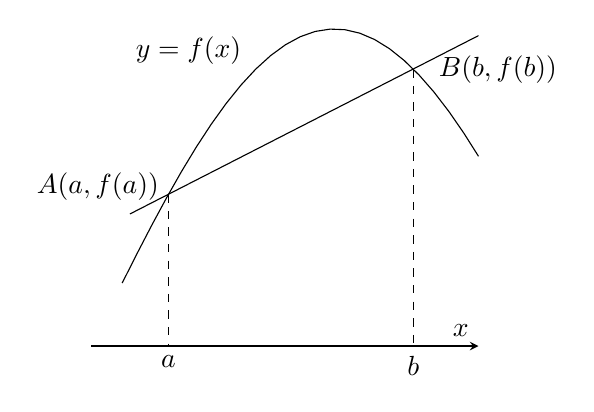
\begin{tikzpicture}
\begin{axis}[clip=false,small,axis lines=middle,xlabel={$x$},xmin=0,ymin=0,xtick={\empty},ytick={\empty},y axis line style={draw=none}]
\addplot[domain=0.2:2.5]{sin(deg(x))}node[pos=0.4,above left]{$y=f(x)$};
\addplot[domain=0.25:2.5]{0.25*x+0.354};
%\draw[] (axis cs:0.49932,0.4788)node[left]{$A$}--(axis cs:2.08,0.873)node[above]{$B$};
\draw[dashed](axis cs:0.49932,0.4788)node[left,yshift={1mm}]{$A(a,f(a))$}--(axis cs:0.49932,0)node[below]{$a$};
\draw[dashed](axis cs:2.08,0.873)node[right,xshift=2mm]{$B(b,f(b))$}--(axis cs:2.08,0)node[below]{$b$};
\end{axis}
\end{tikzpicture}
\caption{وقفہ \عددی{[a,b]} پر \عددی{f} اور قطع \عددی{AB} کے ترسیم۔}
\end{subfigure}\hfill
\begin{subfigure}[t]{0.45\textwidth}
\centering
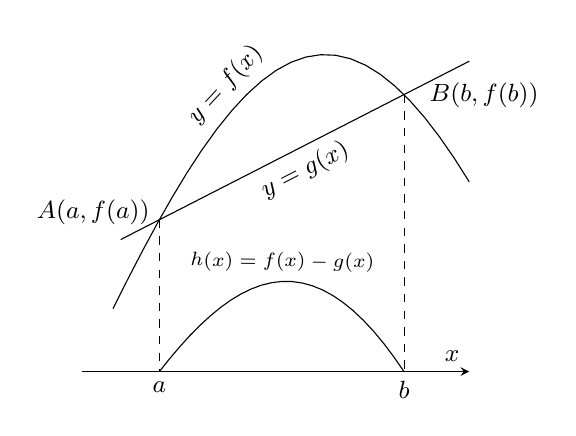
\begin{tikzpicture}[font=\small]
\begin{axis}[clip=false,small,axis lines=middle,xlabel={$x$},xmin=0,ymin=0,xtick={\empty},ytick={\empty},y axis line style={draw=none}]
\addplot[domain=0.2:2.5]{sin(deg(x))}node[pos=0.4,sloped,above]{$y=f(x)$};
\addplot[,domain=0.25:2.5]{0.25*x+0.354}node[pos=0.5,sloped,below]{$y=g(x)$};
\addplot[domain=0.4993:2.08]{sin(deg(x))-0.25*x-0.354}node[pos=0.5,sloped,above,font=\scriptsize]{$h(x)=f(x)-g(x)$};
%\draw[] (axis cs:0.49932,0.4788)node[left]{$A$}--(axis cs:2.08,0.873)node[above]{$B$};
\draw[dashed](axis cs:0.49932,0.4788)node[left,yshift={1mm}]{$A(a,f(a))$}--(axis cs:0.49932,0)node[below]{$a$};
\draw[dashed](axis cs:2.08,0.873)node[right,xshift=2mm]{$B(b,f(b))$}--(axis cs:2.08,0)node[below]{$b$};
\end{axis}
\end{tikzpicture}
\caption{\عددی{f(x)} اور \عددی{g(x)} کے بیچ افقی فاصلہ \عددی{h(x)} ہے۔}
\end{subfigure}
\caption{مسئلہ اوسط قیمت۔}
\label{شکل_مسئلہ_استعمال_اوسط_قیمت}
\end{figure}

تفاعل \عددی{h} وقفہ \عددی{[a,b]} پر مسئلہ رول کو مطمئن کرتا ہے۔ تفاعل \عددی{h} وقفہ \عددی{[a,b]} پر استمراری اور \عددی{(a,b)} پر قابل تفرق  ہے (چونکہ اس وقفہ پر \عددی{f} اور \عددی{g} استمراری اور قابل تفرق ہیں)۔ مزید چونکہ \عددی{f} اور \عددی{g} دونوں نقطہ \عددی{A} اور \عددی{B} سے گزرتے ہیں لہٰذا \عددی{h(a)=h(b)=0} ہے۔ یوں \عددی{(a,b)} میں کسی نقطہ \عددی{c} پر \عددی{h'(x)=0} ہو گا۔ یہ وہ نقطہ ہے جو ہمیں مساوات \حوالہ{مساوات_استعمال_مسئلہ_اوسط_قیمت_الف} میں درکار ہے۔

مساوات \حوالہ{مساوات_استعمال_مسئلہ_اوسط_قیمت_الف} کی تصدیق کی خاطر ہم \عددی{x} کے لحاظ سے مساوات \حوالہ{مساوات_استعمال_مسئلہ_اوسط_قیمت_ج} کے دونوں ہاتھ  کا تفرق لے کر اس میں \عددی{x=c} پر کرتے ہیں۔
\begin{align*}
h'(x)&=f'(x)-\frac{f(b)-f(a)}{b-a}&&\text{\RL{(تفرق)}}\\
h'(c)&=f'(c)-\frac{f(b)-f(a)}{b-a}&& (x=c)\\
0&=f'(c)-\frac{f(b)-f(a)}{b-a}&&(h'(c)=0)\\
f'(c)&=\frac{f(b)-f(a)}{b-a}
\end{align*}
یوں ثبوت مکمل ہوتا ہے۔
\انتہا{ثبوت}
%===============================

دھیان رہے کہ مسئلہ اوسط قیمت میں نقطہ \عددی{a} یا \عددی{b} پر \عددی{f} کا قابل تفرق ہونا ضروری نہیں ہے البتہ ان نقطوں پر \عددی{f} کا استمراری ہونا کافی ہے (شکل \حوالہ{شکل_استعمال_تفرق_ضروری_نہیں})۔
\begin{figure}
\centering
\begin{minipage}{0.45\textwidth}
\centering
\begin{tikzpicture}
\begin{axis}[clip=false,axis equal,small,axis lines=middle,xlabel={$x$},ylabel={y},xtick={-1,1},ytick={1},ymax=1.5,xmin=-1.25,xmax=1.5,ylabel style={at={(current axis.above origin)},anchor=south}]
\addplot[domain=-1:-0.9]{sqrt(1-x^2)};
\addplot[domain=0.9:1]{sqrt(1-x^2)};
\addplot[domain=-0.9:0.9]{sqrt(1-x^2)}node[pos=0.5,above right,align=center]{$y=\sqrt{1-x^2}$ \\   $-1\le x\le 1$};
\addplot[] plot coordinates {(-0.5,1) (0.5,1)};
\end{axis}
\end{tikzpicture}
\caption{
اگرچہ \عددی{y=\sqrt{1-x^2}} نقطہ \عددی{-1} اور \عددی{1} پر نا قابل تفرق ہے یہ \عددی{[-1,1]} پر مسئلہ اوسط قیمت کو مطمئن کرتا ہے۔
}
\label{شکل_استعمال_تفرق_ضروری_نہیں}
\end{minipage}\hfill
\begin{minipage}{0.45\textwidth}
\centering
\begin{tikzpicture}
\begin{axis}[clip=false,axis equal,small,axis lines=middle,xlabel={$x$},ylabel={y},xtick={1,2},ytick={1,4},ylabel style={at={(current axis.above origin)},anchor=south},ymin=-0.2,ymax=5]
\addplot[domain=0:2]{x^2}node[pos=0.7,right]{$y=x^2$};
\addplot[domain=0.7:1.5]{2*x-1};
\draw(axis cs:0,0) node[below left]{$A(0,0)$}--(axis cs:2,4)node[above]{$B(2,4)$};
\draw(axis cs:0,0)node[circ]{} (axis cs:1,1)node[circ]{}node[right]{$(1,1)$}  (axis cs:2,4)node[circ]{};
\end{axis}
\end{tikzpicture}
\caption{نقطہ \عددی{c=1} پر مماس قطع \عددی{AB} کے متوازی ہے (مثال \حوالہ{مثال_استعمال_یہاں_نقطہ_دیکھ_سکتے_ہیں})}
\label{شکل_مثال_استعمال_یہاں_نقطہ_دیکھ_سکتے_ہیں}
\end{minipage}
\end{figure}
 ہم عموماً \عددی{c} کے بارے میں صرف اتنا ہی جانتے ہیں جتنا یہ مسئلہ ہمیں بتاتا ہے، یعنی کہ، \عددی{c} موجود ہے۔اگلی مثال کی طرح بعض اوقات ہم \عددی{c} کو جان پاتے ہیں لیکن ایسا شاذونادر ہو گا۔

\ابتدا{مثال}\شناخت{مثال_استعمال_یہاں_نقطہ_دیکھ_سکتے_ہیں}
وقفہ \عددی{0\le x\le 2} پر تفاعل \عددی{f(x)=x^2} استمراری ہے اور \عددی{0<x<2} پر یہ قابل تفرق ہے (شکل \حوالہ{شکل_مثال_استعمال_یہاں_نقطہ_دیکھ_سکتے_ہیں})۔ چونکہ \عددی{f(0)=0} اور \عددی{f(2)=4} ہیں لہٰذا مسئلہ اوسط قیمت کے تحت اس وقفہ میں نقطہ \عددی{c} پر تفرق \عددی{f'(x)=2x} کی قیمت لازماً \عددی{\tfrac{4-0}{2-0}=2} ہو گی۔ موجودہ مثال میں ہم \عددی{2x=2} کو حل کرتے ہوئے
 \عددی{x=c=1} حاصل کر پاتے ہیں۔ 
\انتہا{مثال}
%=======================

\جزوحصہء{طبعی تشریح}
اگر ہم \عددی{[a,b]} پر \عددی{\tfrac{f(b)-f(a)}{b-a}} کو \عددی{f} کی  اوسط تبدیلی اور \عددی{f'(c)} کو لمحاتی تبدیلی تصور کریں تب مسئلہ اوسط قیمت کہتا ہے کہ کسی اندرونی   نقطہ پر لمحاتی تبدیلی ضرور پورے وقفہ پر اوسط تبدیلی کے برابر ہو گی۔

\ابتدا{مثال}
ایک گاڑی ساکن حال سے شروع ہر کر \عددی{8} سیکنڈوں میں کل \عددی{120} میٹر فاصلہ طے کرتی ہے۔ان \عددی{8} سیکنڈوں کے لئے گاڑی کی اوسط رفتار \عددی{\tfrac{120}{8}=\SI{15}{\meter\per\second}} ہے۔ مسئلہ اوسط قیمت کہتا ہے کہ ان آٹھ سیکنڈوں میں کسی لمحہ رفتار پیما ٹھیک یہی رفتار دکھائے گا۔
\انتہا{مثال}
%=======================


\جزوحصہء{ضمنی نتائج اور چند جوابات}
اس حصہ کے شروع میں ہم نے پوچھا کہ کس تفاعل کا تفرق صفر ہو گا۔مسئلہ اوسط قیمت کا پہلا ضمنی نتیجہ اس کا جواب دیتا ہے۔

\ابتدا{ضمنی نتیجہ}\شناخت{نتیجہ_صریح_استعمال_پہلا}\موٹا{صفر تفرق کے تفاعل مستقل ہوں گے}\\
اگر وقفہ \عددی{I} کے ہر نقطہ پر \عددی{f'(x)=0} ہو تب \عددی{I} میں تمام \عددی{x} پر \عددی{f(x)=C} ہو گا جہاں \عددی{C} مستقل ہے۔
\انتہا{ضمنی نتیجہ}
%=======================

ہم جانتے ہیں کہ اگر وقفہ \عددی{I} پر تفاعل \عددی{f} کی قیمت مستقل ہو تب \عددی{I} پر \عددی{f} قابل تفرق ہو گا اور \عددی{I} میں تمام \عددی{x} پر \عددی{f'(x)=0} ہو گا۔ ضمنی نتیجہ اس کا الٹ پیش کرتا ہے۔

%=================
\ابتدا{ثبوت ضمنی نتیجہ}
ہم دکھانا چاہتے ہیں کہ \عددی{I} پر \عددی{f} کی قیمت مستقل ہے۔ہم \عددی{I} میں ہر دو نقطوں \عددی{x_1} اور \عددی{x_2} پر \عددی{f(x_1)=f(x_2)} دکھاتے ہوئے ایسا کرتے ہیں۔

فرض کریں \عددی{x_1} اور \عددی{x_2} وقفہ \عددی{I} میں کوئی بھی دو نقطے ہیں جن کی شمار بائیں سے دائیں جانب ہے لہٰذا \عددی{x_1<x_2} ہو گا۔یوں \عددی{[x_1,x_2]} پر \عددی{f} مسئلہ اوسط قیمت کو مطمئن کرے گا۔ یہ \عددی{} کے ہر نقطہ پر قابل تفرق ہو گا لہٰذا یہ ہر اس نقطہ پر استمراری بھی ہو گا۔یوں \عددی{x_1} اور \عددی{x_2} کے بیچ کسی نقطہ \عددی{c} پر
\begin{align*}
\frac{f(x_2)-f(x_1)}{x_2-x_1}=f'(c)
\end{align*}
ہو گا۔چونکہ پورے \عددی{I} پر \عددی{f'=0} ہے لہٰذا اس مساوات کو درج ذیل لکھا جا سکتا ہے۔
\begin{align*}
\frac{f(x_2)-f(x_1)}{x_2-x_1}=f'(c),\quad f(x_2)-f(x_1)=0,\quad f(x_1)=f(x_2)
\end{align*}
\انتہا{ثبوت ضمنی نتیجہ}
%==========================

اس حصہ کے شروع میں ہم نے یہ بھی پوچھا کہ کیا ہم اسراع سے پیچھے کی طرف چلتے ہوئے رفتار اور ہٹاو تلاش کر سکتے ہیں۔یہ کا جواب اگلا ضمنی نتیجہ پیش کرتا ہے۔

\ابتدا{ضمنی نتیجہ}\شناخت{نتیجہ_صریح_استعمال_دوم}\موٹا{ایک جیسے تفرق والے تفاعل میں مستقل کا فرق ہو گا}\\
اگر وقفہ \عددی{I} کے ہر نقطہ پر \عددی{f'(x)=g'(x)} ہو تب ایسا مستقل \عددی{C} موجود ہو گا کہ \عددی{I} میں تمام \عددی{x} پر \عددی{f(x)=g(x)+C} ہو۔ 
\انتہا{ضمنی نتیجہ}
%===================
\ابتدا{ثبوت ضمنی نتیجہ}
\عددی{I} میں ہر نقطہ پر تفاعل فرق \عددی{h=f-g} کا تفرق
\begin{align*}
h'(x)=f'(x)-h'(x)=0
\end{align*}
ہو گا۔یوں  ضمنی نتیجہ \حوالہ{نتیجہ_صریح_استعمال_پہلا} کے تحت \عددی{I} پر \عددی{h(x)=C} ہو گا۔یوں \عددی{f(x)-g(x)=C} یا \عددی{f(x)=g(x)+C} ہو گا۔
\انتہا{ثبوت ضمنی نتیجہ}
%=======================

ضمنی نتیجہ \حوالہ{نتیجہ_صریح_استعمال_دوم} کہتا ہے  کہ وقفہ پر دو تفاعل کے فرق کا تفرق صرف اس صورت صفر کے برابر ہو گا جب اس وقفہ پر ان تفاعل کا مستقل فرق ہو۔ مثال کے طور پر ہم جانتے ہیں کہ \عددی{(-\infty,\infty)} پر \عددی{f(x)=x^2} کا تفرق \عددی{2x} ہے۔ایسا دوسرا تفاعل جس کا \عددی{(-\infty,\infty)} پر تفرق \عددی{2x} ہو کا کلیہ لازماً \عددی{x^2+C} ہو گا (شکل \حوالہ{شکل_نتیجہ_صریح_استعمال_دوم})۔
\begin{figure}
\centering
\begin{minipage}{0.45\textwidth}
\centering
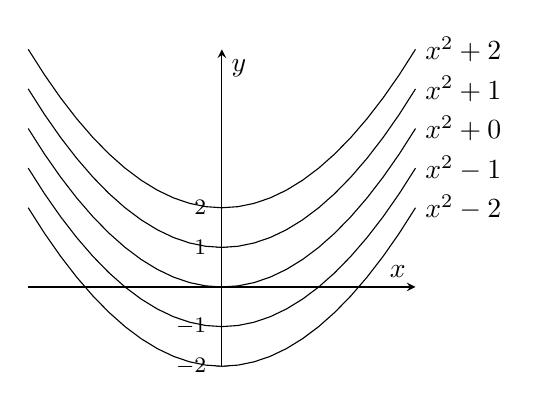
\begin{tikzpicture}
\begin{axis}[clip=false,small,axis lines=middle,xlabel={$x$},ylabel={$y$},ytick={-2,-1,1,2},xtick={\empty}]
\addplot[domain=-2:2]{x^2}node[right]{$x^2+0$};
\addplot[domain=-2:2]{x^2+1}node[right]{$x^2+1$};
\addplot[domain=-2:2]{x^2+2}node[right]{$x^2+2$};
\addplot[domain=-2:2]{x^2-1}node[right]{$x^2-1$};
\addplot[domain=-2:2]{x^2-2}node[right]{$x^2-2$};
\end{axis}
\end{tikzpicture}
\caption{ضمنی نتیجہ \حوالہ{نتیجہ_صریح_استعمال_دوم} کہتا ہے کہ ایک جیسے تفرق والے تفاعل میں صرف انتصابی فرق پایا جاتا ہے۔}
\label{شکل_نتیجہ_صریح_استعمال_دوم}
\end{minipage}\hfill
\begin{minipage}{0.45\textwidth}
\centering
\begin{tikzpicture}
\begin{axis}[clip=false,small,axis lines=middle,xlabel={$x$},ylabel={$y$},ytick={2,3},xtick={\empty},ymin=-0.25,ymax=3.5]
\addplot[domain=-4.713:4.713,smooth]{3-cos(deg(x))}node[left]{$3-\cos x$};
\end{axis}
\end{tikzpicture}
\caption{ترسیم برائے مثال \حوالہ{مثال_استعمال_نتیجہ_صریح_کوسائن}}
\label{شکل_مثال_استعمال_نتیجہ_صریح_کوسائن}
\end{minipage}
\end{figure}

%=======================
\ابتدا{مثال}\شناخت{مثال_استعمال_نتیجہ_صریح_کوسائن}
ایسا تفاعل \عددی{f(x)} تلاش کریں جس کا تفرق \عددی{\sin x} ہو اور جو نقطہ \عددی{(0,2)} سے گزرتا ہو۔\\
حل:\quad
چونکہ \عددی{g(x)=-\cos x} کا تفرق بھی \عددی{\sin x} ہے لہٰذا \عددی{f(x)=-\cos x +C} ہو گا۔دیا گیا نقطہ اس میں پر کرتے ہوئے مستقل \عددی{C}حاصل کرتے ہیں۔
\begin{align*}
f(0)=-\cos(0)+C=2\quad \implies\quad C=3
\end{align*} 
یوں درکار تفاعل \عددی{f(x)=-\cos x+3} ہے (شکل \حوالہ{شکل_مثال_استعمال_نتیجہ_صریح_کوسائن})۔
\انتہا{مثال}
%==============================
\جزوحصہء{اسراع سے سمتی رفتار اور ہٹاو کا حصول}
سطح زمین کے قریب جہاں \عددی{g=\SI{9.8}{\meter\per\second\squared}} ہے ساکن حال سے آزادانہ گرتے ہوئے جسم کی سمتی رفتار اور ہٹاو تلاش کرتے ہیں۔

ہم جانتے ہیں کہ سمتی رفتار \عددی{v} ایسا تفاعل ہے جس کا تفرق \عددی{9.8} کے برابر ہے۔ ہم یہ جانتے ہیں کہ \عددی{g(t)=9.8 t} کا تفرق \عددی{9.8} ہے لہٰذا ضمنی نتیجہ \حوالہ{نتیجہ_صریح_استعمال_دوم} کے تحت
\begin{align*}
v(t)=9.8t+C
\end{align*}
ہو گا جہاں \عددی{C} مستقل ہے۔لمحہ \عددی{t=0} پر جسم ساکن ہو گا لہٰذا
\begin{align*}
v(0)=9.8(0)+C\quad \implies \quad C=0 
\end{align*}
ہو گا۔یوں سمتی رفتار تفاعل \عددی{v(t)=9.8 t} ہو گا۔ ہم یہ بھی جانتے ہیں کہ \عددی{h(t)=4.9t^2} کا تفرق \عددی{9.8t} ہے لہٰذا  ضمنی نتیجہ \حوالہ{نتیجہ_صریح_استعمال_دوم} کے تحت
\begin{align*}
s(t)=4.9t^2+C
\end{align*}
ہو گا جہاں \عددی{C} مستقل ہے۔چونکہ لمحہ \عددی{t=0} پر ہٹاو صفر ہے لہٰذا
\begin{align*}
s(0)=4.9(0^2)+C=0\quad \implies \quad C=0
\end{align*} 
یعنی \عددی{s(t)=4.9t^2} ہو گا۔

کسی تفاعل کی شرح تبدیلی سے تفاعل حاصل کرنے کی صلاحیت، احصاء کی اہم ترین طاقت ہے۔ اس پر مزید بات اگلے باب میں کی جائے گی۔

\جزوحصہء{بڑھتا تفاعل اور گھٹتا تفاعل}
اس حصہ کے شروع میں ہم نے پوچھا کہ کس قسم کے تفاعل کا تفرق مثبت اور کس کا تفرق منفی ہو گا۔مسئلہ اوسط قیمت کا تیسرا ضمنی نتیجہ جو اس کا جواب دیتا ہے کہتا ہے کہ بڑھتے ہوئے تفاعل کا تفرق مثبت اور گھٹے ہوئے تفاعل کا تفرق منفی ہو گا۔

\ابتدا{تعریف}
فرض کریں وقفہ \عددی{I} پر تفاعل \عددی{f} معین ہے اور اس وقفہ پر \عددی{x_1} اور \عددی{x_2} کوئی بھی دو نقطے ہیں۔
\begin{enumerate}[1.]
\item
اگر \عددی{x_1<x_2} کی صورت میں \عددی{f(x_1)<f(x_2)} ہو تب \عددی{I} پر \عددی{f} \اصطلاح{بڑھتا}\فرہنگ{بڑھتا}\حاشیہب{increasing}\فرہنگ{increasing} تفاعل کہلاتا ہے۔
\item
اگر \عددی{x_1<x_2} کی صورت میں \عددی{f(x_1)>f(x_2)} ہو تب \عددی{I} پر \عددی{f} \اصطلاح{گھٹتا}\فرہنگ{گھٹتا}\حاشیہب{decreasing}\فرہنگ{decreasing} تفاعل کہلاتا  ہے۔
\end{enumerate}
\انتہا{تعریف}
%=====================

\ابتدا{ضمنی نتیجہ}\شناخت{نتیجہ_صریح_استعمال_سوم}\موٹا{بڑھتے اور گھٹتے تفاعل کا پہلا تفرقی پرکھ}\\
فرض کریں \عددی{[a,b]} پر \عددی{f} استمراری  اور \عددی{(a,b)} پر \عددی{f} قابل تفرق ہے۔
\begin{itemize}
\item
اگر \عددی{(a,b)} کے ہر نقطہ پر \عددی{f'>0} ہو تب \عددی{[a,b]} پر \عددی{f} بڑھتا ہے۔
\item
اگر \عددی{(a,b)} کے ہر نقطہ پر \عددی{f'<0} ہو تب \عددی{[a,b]} پر \عددی{f} گھٹتا ہے۔
\end{itemize}
\انتہا{ضمنی نتیجہ}
%==============================
\ابتدا{ثبوت ضمنی نتیجہ}
فرض کریں \عددی{[a,b]} میں \عددی{x_1} اور \عددی{x_2} کوئی دو نقطے ہیں جہاں \عددی{x_1<x_2} ہے۔ وقفہ \عددی{[x_1,x_2]} پر مسئلہ اوسط قیمت تفاعل \عددی{f} کے لئے کہتا ہے کہ
\begin{align}\label{مساوات_استعمال_نتیجہ_صریح_سوم_الف}
f(x_2)-f(x_1)=f'(c)(x_2-x_1)
\end{align}
ہو گا جہاں \عددی{x_1} اور \عددی{x_2} کے بیچ \عددی{c} ایک موزوں نقطہ ہے۔ چونکہ \عددی{x_2-x_1} مثبت قیمت ہے لہٰذا مساوات \حوالہ{مساوات_استعمال_نتیجہ_صریح_سوم_الف} کے دائیں ہاتھ کی علامت وہی ہو گی جو \عددی{f'(c)} کی ہے۔یوں \عددی{(a,b)} پر مثبت \عددی{f'(c)} کی صورت میں \عددی{f(x_2)>f(x_1)} ہو گا جبکہ \عددی{(a,b)} پر منفی \عددی{f'(c)} کی صورت میں \عددی{f(x_1)<f(x_2)} ہو گا۔
\انتہا{ثبوت ضمنی نتیجہ}
%==============================

\ابتدا{مثال}\شناخت{مثال_استعمال_بڑھتا_گھٹتا}
وقفہ \عددی{(-\infty,0)} پر تفاعل \عددی{f(x)=x^2} کا تفرق \عددی{f'(x)=2x<0} ہے لہٰذا اس وقفے پر \عددی{f} گھٹے گا۔ وقفہ \عددی{(0,\infty)} پر تفاعل \عددی{f(x)=x^2} کا تفرق \عددی{f'(x)=2x>0} ہے لہٰذا اس وقفے پر \عددی{f} بڑھے گا (شکل \حوالہ{شکل_مثال_استعمال_بڑھتا_گھٹتا})۔
\begin{figure}
\centering
\begin{tikzpicture}[font=\small]
\begin{axis}[clip=false,small,axis lines=middle,xlabel={$x$},ylabel={$y$},xtick={-2,-1,1,2},ytick={1,2,3,4},xmin=-2.5,xmax=2.5,ymax=4.9]
\addplot[domain=-2:2]{x^2}node[left]{$y=x^2$}node[pos=0.15,below left,align=center]{\RL{گھٹتا تفاعل}\\  $y'<0$}node[pos=0.85,below right,align=center]{\RL{بڑھتا تفاعل}\\  $y'>0$}node[pos=0.5,pin=-45:{$y'=0$}]{};
\end{axis}
\end{tikzpicture}
\caption{ترسیم برائے مثال \حوالہ{مثال_استعمال_بڑھتا_گھٹتا}}
\label{شکل_مثال_استعمال_بڑھتا_گھٹتا}
\end{figure}
\انتہا{مثال}
%==================

\حصہء{سوالات}
\موٹا{مسئلہ اوسط قیمت میں \عددی{c} کی تلاش}\\
سوال \حوالہ{سوال_استعمال_موزوں_الف} تا سوال \حوالہ{سوال_استعمال_موزوں_ب} میں دیے وقفہ اور تفاعل کے لئے  \عددی{c} کی ایسی قیمت  تلاش کریں جو مسئلہ اوسط قیمت کے نتیجہ 
\begin{align*}
\frac{f(b)-f(a)}{b-a}=f'(c)
\end{align*}
کو مطمئن کرتی ہو۔

\ابتدا{سوال}\شناخت{سوال_استعمال_موزوں_الف}
$f(x)=x^2+2x-1,\quad [0,1]$\\
جواب:\quad
$\tfrac{1}{2}$
\انتہا{سوال}
%=======================
\ابتدا{سوال}
$f(x)=x^{2/3},\quad [0,1]$
\انتہا{سوال}
%========================
\ابتدا{سوال}
$f(x)=x+\tfrac{1}{x},\quad [\tfrac{1}{2},2]$\\
جواب:\quad
$1$
\انتہا{سوال}
%========================
\ابتدا{سوال}\شناخت{سوال_استعمال_موزوں_ب}
$f(x)=\sqrt{x-1},\quad [1,3]$
\انتہا{سوال}
%========================
\موٹا{قیاس کی پرکھ اور استعمال}\\
سوال \حوالہ{سوال_استعمال_قیاس_الف} تا سوال \حوالہ{سوال_استعمال_قیاس_ب} میں کون سے تفاعل دیے وقفہ پر مسئلہ اوسط قیمت کے قیاس کو مطمئن کرتے ہیں اور کون سے تفاعل ایسا نہیں کرتے ہیں۔ اپنے جواب کی وجہ پیش کریں۔ 

\ابتدا{سوال}\شناخت{سوال_استعمال_قیاس_الف}
$f(x)=x^{2/3},\quad [-1,8]$\\
جواب:\quad
نہیں کرتا؛ دائرہ کار کے اندرونی نقطہ \عددی{x=0} پر \عددی{f} نا قبل تفرق ہے۔ 
\انتہا{سوال}
%==========================
\ابتدا{سوال}
$f(x)=x^{4/5},\quad [0,1]$
\انتہا{سوال}
%===========================
\ابتدا{سوال}
$f(x)=\sqrt{x(1-x)},\quad [0,1]$\\
جواب:\quad
کرتا ہے۔
\انتہا{سوال}
%===========================
\ابتدا{سوال}\شناخت{سوال_استعمال_قیاس_ب}
$f(x)=\begin{cases} \tfrac{\sin x}{x},&-\pi\le x< 0\\ 0,&x=0 \end{cases}$
\انتہا{سوال}
%===========================
\ابتدا{سوال}
درج ذیل تفاعل \عددی{x=0} اور \عددی{x=1} پر صفر کے برابر ہے اور \عددی{(0,1)} پر قابل تفرق ہے لیکن \عددی{(a,b)} پر اس کا تفرق کبھی بھی صفر نہیں ہے۔ 
\begin{align*}
f(x)=\begin{cases} x,& 0\le x<1\\ 0,&x=1 \end{cases}
\end{align*}
ایسا کیوں ممکن ہے؟ کیا مسئلہ رول نہیں کہتا کہ \عددی{(0,1)} پر کہیں تفرق صفر ہو گا؟ اپنے جواب کی وجہ پیش کریں۔
\انتہا{سوال}
%====================
\ابتدا{سوال}
وقفہ \عددی{[0,2]} پر \عددی{a}، \عددی{m} اور \عددی{b} کی کون سی قیمتوں کے لئے  درج ذیل تفاعل مسئلہ اوسط قیمت کی قیاس کو مطمئن کرتا ہے؟
\begin{align*}
f(x)=\begin{cases} 3,&x=0\\ -x^2+3x+a,&0<x<1\\ mx+b,&1\le x\le 2  \end{cases}
\end{align*}
\انتہا{سوال}
%======================
\موٹا{جذر (صفر)}

\ابتدا{سوال}\شناخت{سوال_استعمال_جذر_الف}

\begin{enumerate}[a.]
\item
باری باری درج ذیل کثیر رکنیوں کے صفر کو ایک لکیر پر ترسیم کریں۔ساتھ ہی ان کے یک رتبی تفرق کے  صفر بھی ترسیم کریں۔
\begin{enumerate}[1.]
\item
$y=x^2-4$
\item
$y=x^2+8x+15$
\item
$y=x^3-3x^2+4=(x+1)(x-2)^2$
\item
$y=x^3-33x^2+216x=x(x-9)(x-24)$
\end{enumerate}
\item
مسئلہ رول کی مدد سے ثابت کریں کہ 
$x^n+a_{n-1}x^{n-1}+\cdots+a_1x+a_0$
کے ہر دو صفر کے بیچ \\
$nx^{n-1}+(n-1)a_{n-1}x^{n-2}+\cdots+a_1$
کا ایک صفر پایا جاتا ہے۔
\end{enumerate}
جواب:\quad 
(ا) شکل \حوالہ{شکل_سوال_استعمال_جذر_الف}
\begin{figure}
\centering
\begin{tikzpicture}
\draw[-latex](0,0)node[left]{$(1)$}--++(7,0)node[right]{$x$};
\draw[-latex](0,-1)node[left]{$(2)$}--++(7,0)node[right]{$x$};
\draw[-latex](0,-2)node[left]{$(3)$}--++(7,0)node[right]{$x$};
\foreach \x/\s in {3/-2,4/0,5/2}{\draw(\x,0)node[circ]{}node[below]{$\s$}--++(0,0.1);}
\foreach \x/\s in {3/-5,4/-4,5/-3}{\draw(\x,-1)node[circ]{}node[below]{$\s$}--++(0,0.1);}
\foreach \x/\s in {1/0,2/4,3/9,5/18,6/24}{\draw(\x,-2)node[circ]{}node[below]{$\s$}--++(0,0.1);}
\end{tikzpicture}
\caption{حل ترسیم سوال \حوالہ{سوال_استعمال_جذر_الف}}
\label{شکل_سوال_استعمال_جذر_الف}
\end{figure}
\انتہا{سوال}
%=====================
\ابتدا{سوال}
فرض کریں کہ وقفہ \عددی{[a,b]} میں \عددی{f'''} استمراری ہے اور اس وقفہ پر \عددی{f} کے تین صفر پائے جاتے ہیں۔دکھائیں کہ اس وقفہ پر \عددی{f''} کا کم سے کم ایک صفر پایا جائے گا۔ اس نتیجہ کو عمومی بنائیں۔
\انتہا{سوال}
%=========================
\ابتدا{سوال}
دکھائیں کہ اگر پورے \عددی{[a,b]} پر \عددی{f''>0}  ہو تب \عددی{[a,b]} میں \عددی{f'} کا زیادہ سے زیادہ ایک صفر پایا جائے گا۔اگر \عددی{[a,b]} پر \عددی{f''<0} ہو تب کیا ہو گا؟
\انتہا{سوال}
%=====================
\ابتدا{سوال}
دکھائیں کہ کعبی کثیر رکنی کے صفروں کی زیادہ سے زیادہ تعداد تین ممکن ہے۔
\انتہا{سوال}
%================================

\موٹا{نظریہ اور مثالیں}\\
\ابتدا{سوال}
دکھائیں کہ دو گھنٹوں کی صفر میں کسی لمحہ پر گاڑی کا رفتار پیما ضرور دو گھنٹوں کی اوسط رفتار دکھائے گا۔
\انتہا{سوال}
%====================
\ابتدا{سوال}\ترچھا{تبدیلی درجہ حرارت}\quad
برف سے حرارت پیما کو نکال کر ابلتے  ہوئے پانی میں رکھنے سے اس کا درجہ حرارت \عددی{14} سیکنڈوں میں \عددی{\SI{-19}{\celsius}} سے بڑھ کر \عددی{\SI{100}{\celsius}} ہوتا ہے۔ دکھائیں کہ اس دوران درجہ حرارت میں تبدیلی کی شرح کسی لمحے پر \عددی{\SI{8.5}{\celsius\per\second}} ضرور ہو گی۔ 
\انتہا{سوال}
%====================
\ابتدا{سوال}
فرض کریں کہ وقفہ \عددی{[0,1]} پر قابل تفرق تفاعل \عددی{f} کا تفرق کبھی صفر نہیں ہوتا ہے۔دکھائیں کہ \عددی{f(0\ne f(1)} ہو گا۔ 
\انتہا{سوال}
%===================
\ابتدا{سوال}
دکھائیں کہ \عددی{a} اور \عددی{b} کی کسی بھی قیمتوں کے لئے \عددی{\abs{\sin b-\sin a}\le\abs{b-a}} ہو گا۔
\انتہا{سوال}
%======================
\ابتدا{سوال}
فرض کریں \عددی{[a,b]} پر \عددی{f} قابل تفرق ہے اور \عددی{f(b)<f(a)} ہے۔ کیا \عددی{[a,b]} پر \عددی{f'} کی قیمت کے بارے میں کچھ کہنا ممکن ہو گا؟
\انتہا{سوال}
%=========================
\ابتدا{سوال}
فرض کریں \عددی{[a,b]} پر \عددی{f} اور \عددی{g} قابل تفرق ہیں اور \عددی{f(a)=g(a)} اور \عددی{f(b)=g(b)} ہیں۔دکھائیں کہ \عددی{a} اور \عددی{b} کے بیچ کم سے کم ایسا ایک نقطہ پایا جاتا ہے جہاں \عددی{f} اور \عددی{g} کی ترسیمات کے مماس آپس میں متوازی ہیں۔
\انتہا{سوال}
%==========================
\ابتدا{سوال}
فرض کریں \عددی{x} کی ہر قیمت کے لئے \عددی{f} قابل تفرق ہے۔مزید فرض کریں کہ \عددی{f(1)=1} ہے اور  \عددی{(-\infty,1)} پر  \عددی{f'<0} ہے اور \عددی{(1,\infty)} پر \عددی{f'>0} ہے۔
\begin{enumerate}[a.]
\item
دکھائیں کہ تمام \عددی{x} پر \عددی{f(x)\ge 1} ہو گا۔
\item
کیا \عددی{f'(1)=0} لازماً ہو گا؟ وجہ پیش کریں۔

\end{enumerate}
\انتہا{سوال}
%===========================
\ابتدا{سوال}
فرض کریں \عددی{f(x)=px^2+qx+r} بند وقفہ \عددی{[a,b]} پر معین ہے۔دکھائیں کہ \عددی{(a,b)} میں ٹھیک ایک نقطہ \عددی{c} پر \عددی{f} مسئلہ اوسط قیمت  کے نتیجہ پر پورا اترتا ہے۔ 
\انتہا{سوال}
%============================
\ابتدا{سوال}\ترچھا{حیرت کن ترسیم}\quad
درج ذیل تفاعل ترسیم کریں۔
\begin{align*}
f(x)=\sin x\sin(x+2)-\sin^2(x+1)
\end{align*}
یہ ترسیم کیا کرتی ہے؟ یہ تفاعل اس طرح کا رویہ کیوں رکھتا ہے؟ اپنے جواب کی وجہ پیش کریں۔
\انتہا{سوال}
%=========================
\ابتدا{سوال}
اگر دو تفاعل \عددی{f(x)} اور \عددی{g(x)} کی ترسیمات مستوی میں ایک ہی نقطہ سے شروع ہوتے ہوں اور ہر نقطہ پر ان کی شرح تبدیلی ایک جیسی ہو تب کیا یہ تفاعل بالکل ایک جیسے نہیں ہوں گے؟ اپنے جواب کہ وجہ پیش کریں۔ 
\انتہا{سوال}
%=======================
\ابتدا{سوال}
\begin{enumerate}[a.]
\item
دکھائیں کہ تفاعل \عددی{g(x)=\tfrac{1}{x}} اپنے دائرہ کار کے ہر وقفہ میں گھٹتا ہے۔
\item
اگر جزو (ا) کا نتیجہ درست ہو تب \عددی{g(1)=1} کس طرح \عددی{g(-1)=-1} سے بڑا ہو سکتا ہے؟
\end{enumerate}
\انتہا{سوال}
%=========================
\ابتدا{سوال}\شناخت{سوال_استعمال_مسئلہ_اوسط_قیمت_الف}
فرض کریں وقفہ \عددی{[a,b]} میں تفاعل \عددی{f} معین ہے۔ درج ذیل کو مطمئن کرنے کی خاطر \عددی{f} پر کون سے شرائط لاگو کرنے ہوں گے
\begin{align*}
f'\,\text{\RL{کم سے کم}}\le \frac{f(b)-f(a)}{b-a}\le f'\,\text{\RL{زیادہ سے زیادہ}}
\end{align*} 
جہاں کم سے کم \عددی{f'} اور زیادہ سے زیادہ \عددی{f'} سے مراد \عددی{[a,b]} پر بالترتیب \عددی{f'} کی  کم سے کم اور زیادہ سے زیادہ قیمت ہے۔
\انتہا{سوال}
%=================
\ابتدا{سوال}
اگر \عددی{0\le x\le 0.1} پر \عددی{f'(x)=1/(1+x^4\cos x)} ہو اور \عددی{f(0)=1} ہو تب سوال \حوالہ{سوال_استعمال_مسئلہ_اوسط_قیمت_الف} کی عدم مساوات استعمال کرتے ہوئے  \عددی{f(0.1)} کی تخمینی قیمت تلاش کریں۔\\
جواب:\quad
$1.09999\le f(0.1)\le 1.1$
\انتہا{سوال}
%===================
\ابتدا{سوال}
اگر \عددی{0\le x\le 0.1} پر \عددی{f'(x)=1/(1-x^4)} ہو اور \عددی{f(0)=2} ہو تب سوال \حوالہ{سوال_استعمال_مسئلہ_اوسط_قیمت_الف} کی عدم مساوات استعمال کرتے ہوئے  \عددی{f(0.1)} کی تخمینی قیمت تلاش کریں۔
\انتہا{سوال}
%===================
\ابتدا{سوال}\ترچھا{ہندسی اوسط۔} \quad
دو مثبت اعداد \عددی{a} اور \عددی{b} کی \اصطلاح{ہندسی اوسط}\فرہنگ{اوسط!ہندسی}\حاشیہب{geometric mean}\فرہنگ{mean!geometric} سے مراد عدد \عددی{\sqrt{ab}} ہے۔دکھائیں کہ  مسئلہ اوسط قیمت کے نتیجہ میں مثبت اعداد کے وقفہ \عددی{[a,b]}  پر تفاعل \عددی{f(x)=\tfrac{1}{x}} کے لئے \عددی{c} کی قیمت \عددی{\sqrt{ab}} ہے۔ 
\انتہا{سوال}
%=======================
\ابتدا{سوال}\ترچھا{حسابی اوسط۔}\quad
دو اعداد \عددی{a} اور \عددی{b} کی \اصطلاح{حسابی اوسط}\فرہنگ{اوسط!حسابی}\حاشیہب{arithmetic mean}\فرہنگ{mean!arithmetic} \عددی{\tfrac{a+b}{2}} ہے۔ دکھائیں کہ مسئلہ اوسط قیمت میں وقفہ \عددی{[a,b]} پر تفاعل \عددی{f(x)=x^2} کے لئے \عددی{c} کی قیمت \عددی{\tfrac{a+b}{2}} ہو گی۔
\انتہا{سوال}
%=========================
\موٹا{تفرق سے تفاعل کا حصول}\\
\ابتدا{سوال}
فرض کریں \عددی{f(-1)=3} اور تمام \عددی{x} کے لئے \عددی{f'(x)=0} ہے۔ کیا تمام \عددی{x} کے لئے \عددی{f(x)=3} ہو گا؟ اپنے جواب کی وجہ پیش کریں۔\\
جواب:\quad 
ہاں
\انتہا{سوال}
%===================
\ابتدا{سوال}
فرض کریں \عددی{f(0)=5} اور تمام \عددی{x} کے لئے \عددی{f'(x)=2} ہیں۔ کیا تمام \عددی{x} کے لئے \عددی{f(x)=2x+5} ہو گا؟ اپنے جواب کی وجہ پیش کریں۔
\انتہا{سوال}
%=====================
\ابتدا{سوال}
فرض کریں تمام \عددی{x} کے لئے \عددی{f'(0)=2x} ہے۔ درج ذیل صورتوں میں \عددی{f(2)} تلاش کریں۔
\begin{multicols}{3}
\begin{enumerate}[a.]
\item
$f(0)=0$
\item
$f(1)=0$
\item
$f(-2)=3$
\end{enumerate}
\end{multicols}
جواب:\quad
(ا) \عددی{4}، (ب) \عددی{3}، (ج) \عددی{3}
\انتہا{سوال}
%========================
\ابتدا{سوال}
جن تفاعل کا تفرق مستقل ہو ان کے بارے میں کیا کہا جا سکتا ہے؟ اپنے جواب کی وجہ پیش کریں۔
\انتہا{سوال}
%=========================
سوال \حوالہ{سوال_استعمال_تفرق_سے_تفاعل_الف}  تا سوال \حوالہ{سوال_استعمال_تفرق_سے_تفاعل_ب} میں وہ تفاعل تلاش کریں جس کا تفرق دیا گیا ہے۔

\ابتدا{سوال}\شناخت{سوال_استعمال_تفرق_سے_تفاعل_الف}
(ا) \عددی{y'=x}، (ب) \عددی{y'=x^2}، (ج) \عددی{y'=x^3}\\
جواب:\quad
(ا) \عددی{\tfrac{x^2}{2}+C}، (ب) \عددی{\tfrac{x^3}{3}+C}، (ج) \عددی{\tfrac{x^4}{4}+C}
\انتہا{سوال}
%=========================
\ابتدا{سوال}
(ا) \عددی{y'=2x}، (ب) \عددی{y'=2x-1}، (ج) \عددی{y'=3x^2+2x-1}
\انتہا{سوال}
%======================
\ابتدا{سوال}
(ا) \عددی{y'=-\tfrac{1}{x^2}}، (ب) \عددی{y'=1-\tfrac{1}{x^2}}، (ج) \عددی{y'=5+\tfrac{1}{x^2}}\\
جواب:\quad
(ا) \عددی{\tfrac{1}{x}+C}، (ب) \عددی{x+\tfrac{1}{x}+C}، (ج) \عددی{5x-\tfrac{1}{x}+C}
\انتہا{سوال}
%==========================
\ابتدا{سوال}
(ا) \عددی{y'=\tfrac{1}{2\sqrt{x}}}، (ب) \عددی{y'=\tfrac{1}{\sqrt{x}}}، (ج) \عددی{y'=4x-\tfrac{1}{\sqrt{x}}}
\انتہا{سوال}
%==========================
\ابتدا{سوال}
(ا) \عددی{y'=\sin 2t}، (ب) \عددی{y'=\cos \tfrac{t}{2}}، (ج) \عددی{y'=\sin 2t+\cos \tfrac{t}{2}}\\
جواب:\quad
(ا) \عددی{-\tfrac{1}{2}\cos 2t+C}، (ب) \عددی{2\sin\tfrac{t}{2}+C}، (ج) \عددی{-\tfrac{1}{2}\cos 2t+2\sin\tfrac{t}{2}+C}
\انتہا{سوال}
%===========================
\ابتدا{سوال}\شناخت{سوال_استعمال_تفرق_سے_تفاعل_ب}
(ا) \عددی{y'=\sec^2 \theta}، (ب) \عددی{y'=\sqrt{\theta}}، (ج) \عددی{y'=\sqrt{\theta}-\sec^2\theta}
\انتہا{سوال}
%=========================
سوال \حوالہ{سوال_استعمال_تفرق_نقطہ_الف} تا سوال \حوالہ{سوال_استعمال_تفرق_نقطہ_ب} میں وہ تفاعل تلاش کریں جس کا تفرق دیا گیا ہے اور جو دیے گئے  نقطہ سے گزرتا ہے۔

\ابتدا{سوال}\شناخت{سوال_استعمال_تفرق_نقطہ_الف}
$f'(x)=2x-1,\quad N(0,0)$\\
جواب:\quad
$f(x)=x^2-x$
\انتہا{سوال}
%====================
\ابتدا{سوال}
$g'(x)=\tfrac{1}{x^2}+2x,\quad N(-1,1)$
\انتہا{سوال}
%====================
\ابتدا{سوال}
$r'(\theta)=8-\csc^2\theta,\quad N(\tfrac{\pi}{4},0)$\\
جواب:\quad
$r(\theta)=8\theta+\cot \theta-2\pi-1$
\انتہا{سوال}
%========================
\ابتدا{سوال}\شناخت{سوال_استعمال_تفرق_نقطہ_ب}
$r'(t)=\sec t\tan t-1,\quad N(0,0)$
\انتہا{سوال}
%===========================
\موٹا{صفروں  کی گنتی}\\
مساوات \عددی{f(x)=0} کو اعدادی طریقہ سے حل کرنے سے پہلے ہم عموماً  مطلوبہ وقفہ پر  مساوات کی متوقع صفروں کی تعداد جاننا چاہتے ہیں۔ بعض اوقات ضمنی نتیجہ \حوالہ{نتیجہ_صریح_استعمال_سوم} کی مدد سے ایسا کرنا ممکن ہو گا۔

درج ذیل فرض کریں۔
\begin{enumerate}[1.]
\item
\عددی{[a,b]} پر \عددی{f} استمراری اور \عددی{(a,b)} پر قابل تفرق ہے۔
\item
\عددی{f(a)} اور \عددی{f(b)} کی علامتیں ایک دوسرے کی الٹ ہیں۔
\item
پورے \عددی{(a,b)} پر \عددی{f'>0} اور یا پورے \عددی{(a,b)} پر \عددی{f'<0} ہے۔
\end{enumerate}
تب \عددی{a} اور \عددی{b} کے بیچ \عددی{f} کا ٹھیک ایک صفر پایا جائے گا۔چونکہ یہ پورے \عددی{[a,b]} پر بڑھ رہا ہے اور یا  پورے \عددی{[a,b]} پر گھٹ رہا ہے لہٰذا یہ \عددی{x} محور کو ایک ہی بار قطع کر سکتا ہے۔اس کے باوجود مسئلہ \حوالہ{مسئلہ_حد_متوسط_قیمت} کے تحت اس کا کم سے کم ایک صفر ہو گا۔ مثال کے طور پر \عددی{[-1,1]} پر \عددی{f(x)=x^3+3x+1} قابل تفرق ہے، \عددی{f(-1)=-3} اور \عددی{f(1)=5} کی علامتیں ایک دوسرے کی الٹ ہیں، اور تمام \عددی{x} کے لئے \عددی{f'(x)=3x^2+3>0} ہے  لہٰذا \عددی{[-1,1]} پر \عددی{f} کا ٹھیک ایک صفر پایا جاتا ہے (شکل \حوالہ{شکل_استعمال_یک_صفر_مثال})۔
\begin{figure}
\centering
\begin{tikzpicture}[font=\small]
\begin{axis}[small,axis lines=middle,xlabel={$x$},ylabel={$y$},xtick={-1,1},ytick={-3,1,5},xlabel style={at={(current axis.right of origin)},anchor=west}]
\addplot[domain=-1.25:1.25]{x^3+3*x+1};
\draw(axis cs:-0.322,0)node[circ]{};
\draw(axis cs:0,1)node[right]{$y=x^3+3x+1$};
\end{axis}
\end{tikzpicture}
\caption{کثیر رکنی \عددی{y=x^3+3x+1} کا واحد صفر دکھایا گیا ہے۔}
\label{شکل_استعمال_یک_صفر_مثال}
\end{figure}

سوال \حوالہ{سوال_استعمال_صرف_ایک_صفر_الف} تا سوال \حوالہ{سوال_استعمال_صرف_ایک_صفر_ب} میں دکھائیں کہ دیے گئے وقفہ پر تفاعل کا صرف ایک صفر پایا جاتا ہے۔

\ابتدا{سوال}\شناخت{سوال_استعمال_صرف_ایک_صفر_الف}
$f(x)=x^4+3x+1,\quad [-2,-1]$
\انتہا{سوال}
%===========================
\ابتدا{سوال}
$f(x)=x^3+\tfrac{4}{x^2}+7,\quad (-\infty,0)$
\انتہا{سوال}
%=============================
\ابتدا{سوال}
$g(t)=\sqrt{t}+\sqrt{1+t}-4,\quad (0,\infty)$
\انتہا{سوال}
%=============================
\ابتدا{سوال}
$g(t)=\tfrac{1}{1-t}+\sqrt{1+t}-3,\quad (-1,1)$
\انتہا{سوال}
%=============================
\ابتدا{سوال}
$r(\theta)=\theta+\sin^2(\tfrac{\theta}{3})-8,\quad (-\infty,\infty)$
\انتہا{سوال}
%=============================
\ابتدا{سوال}
$r(\theta)=2\theta-\cos^2\theta+\sqrt{2},\quad (-\infty,\infty)$
\انتہا{سوال}
%=============================
\ابتدا{سوال}
$r(\theta)=\sec\theta-\tfrac{1}{\theta^3}+5,\quad (0,\tfrac{\pi}{2})$
\انتہا{سوال}
%=============================
\ابتدا{سوال}\شناخت{سوال_استعمال_صرف_ایک_صفر_ب}
$r(\theta)=\tan\theta-\cot\theta-\theta,\quad (0,\tfrac{\pi}{2})$
\انتہا{سوال}
%=============================
\موٹا{کمپیوٹر کا استعمال}\\
\ابتدا{سوال}
\begin{enumerate}[a.]
\item
ایسا کثیر رکنی \عددی{f(x)} تشکیل دیں جس کے صفر \عددی{x=-2,-1,0,1,2} پر پائے جاتے ہوں۔
\item
\عددی{f(x)} اور \عددی{f'(x)} کو ایک ساتھ ترسیم کریں۔ آپ کو کیا خوبی نظر آتی ہے۔
\item
کیا \عددی{g(x)=\sin x} اور اس کا تفرق \عددی{g'(x)}  بھی ایسی خوبی رکھتے ہیں؟
\end{enumerate}
\انتہا{سوال}
%=======================

\حصہ{مقامی انتہائی قیمتوں کا یک رتبی تفرقی پرکھ}\شناخت{حصہ_استعمال_مقامی_انتہا_کا_یک_درجی_تفرقی_پرکھ}
اس حصہ میں مقامی انتہائی قیمت کی موجودگی کے لئے تفاعل کے نقطہ فاصل  کو پرکھنا دکھایا جائے گا۔ 

\جزوحصہ{پرکھ}
جیسا شکل \حوالہ{شکل_استعمال_بعض_انتہا_بعض_نہیں} میں دکھایا گیا ہے تفاعل \عددی{f}  کے بعض نقطہ فاصل  پر تفاعل کی مقامی انتہا پائی جائے گی اور بعض پر نہیں۔یہ راز نقطہ کے بالکل قریب  \عددی{f'} کی علامت میں پوشیدہ ہے۔ جیسا جیسا \عددی{x} بائیں سے دائیں رخ بڑھتا ہے \عددی{f} کی قیمت وہاں بڑھتی ہے جہاں \عددی{f'>0} ہو اور \عددی{f} کی قیمت وہاں گھٹتی ہے جہاں \عددی{f'<0} ہو۔
\begin{figure}
\centering
\begin{tikzpicture}[font=\small]
\draw[-latex](-1,0)--(10,0)node[right]{$x$};
\draw(0,0.5) to [out=10,in=180] node[pos=0.5,right]{$f'>0$}(1.5,2) to [out=0,in=180]node[pos=0.5,right]{$f'>0$} (3,3.5) to [out=0,in=180]node[pos=0.65,left]{$f'<0$} (4.5,1.6) to [out=0,in=-135] node[pos=0.5,right]{$f'>0$}(6,4) to[out=-80,in=180] node[pos=0.7,left,yshift=-1mm]{$f'<0$}(7.5,3) to [out=0,in=100]node[pos=0.5,left,yshift=-1mm]{$f'<0$}(9,1.2);
\draw(1,2)--(2,2)node[pos=0.5,above,align=center]{\RL{انتہا نہیں}\\ $f'=0$};
\draw(2.5,3.5)--(3.5,3.5)node[pos=0.5,above,align=center]{\RL{مقامی زیادہ سے زیادہ}\\ $f'=0$};
\draw(4,1.6)--(5,1.6)node[pos=0.5,below,align=center]{$f'=0$\\   \RL{مقامی کم سے کم}};
\draw(5.5,4)--(6.5,4)node[pos=0.5,above,align=center]{\RL{مطلق زیادہ سے زیادہ}\\   \RL{$f'$ غیر معین}};
\draw(7,3)--(8,3)node[pos=0.5,above,align=center]{\RL{انتہا نہیں}\\  $f'=0$};
\draw(0,0.5)node[left]{\RL{مطلق کم سے کم}};
\draw(9,1.2)node[right]{\RL{مقامی کم سے کم}};
\draw[dashed] (0,0.5)--(0,0)node[below]{$a$}   (1.5,2)--(1.5,0)node[below]{$c_1$}  (3,3.5)--(3,0)node[below]{$c_2$}  (4.5,1.6)--(4.5,0)node[below]{$c_3$}  (6,4)--(6,0)node[below]{$c_4$}  (7.5,3)--(7.5,0)node[below]{$c_5$}  (9,1.2)--(9,0)node[below]{$b$};
\end{tikzpicture}
\caption{بعض نقطہ فاصل پر مقامی انتہا پائی جاتی ہے اور بعض پر نہیں۔}
\label{شکل_استعمال_بعض_انتہا_بعض_نہیں}
\end{figure}

آپ (شکل \حوالہ{شکل_استعمال_بعض_انتہا_بعض_نہیں} سے) دیکھ سکتے ہیں  کہ مقامی کم سے کم نقطہ پر نقطہ کے بالکل بائیں \عددی{f'<0} جبکہ نقطہ کے بالکل دائیں \عددی{f'>0} ہو گا۔ ( آخری نقطہ کی صورت میں نقطہ کے صرف ایک طرف پر \عددی{f'} کی قیمت دیکھی جا سکتی ہے۔) یوں مقامی کم سے کم نقطہ کے بالکل بائیں تفاعل کی قیمت گھٹتی ہے (یعنی ترسیم نیچے گرتی ہے) جبکہ اس نقطہ کے بالکل دائیں تفاعل کی قیمت بڑھتی ہے (یعنی ترسیم اوپر اٹھتی ہے)۔  اسی طرح مقامی زیادہ سے زیادہ  نقطہ پر نقطہ کے بالکل بائیں \عددی{f'>0} جبکہ نقطہ کے بالکل دائیں \عددی{f'<0} ہو گا۔یوں اس نقطہ کے بالکل بائیں تفاعل کی قیمت بڑھتی ہے (یعنی ترسیم اوپر اٹھتی ہے) جبکہ اس نقطہ کے بالکل دائیں تفاعل کی قیمت گھٹتی ہے (یعنی ترسیم نیچے گرتی ہے)۔

اس مشاہدہ سے مقامی انتہائی قیمت کی موجودگی کا  پرکھ  حاصل ہوتا ہے۔

\ابتدا{مسئلہ}\شناخت{مسئلہ_استعمال_پرکھ_مقامی_انتہائی}\موٹا{مقامی انتہائی قیمت کا یک رتبی تفرقی پرکھ}\\
درج ذیل پرکھ استمراری تفاعل \عددی{f(x)} کے لئے ہیں۔

\موٹا{نقطہ فاصل \عددی{c} پر:}
\begin{enumerate}
\item
اگر \عددی{c} پر \عددی{f'} کی علامت مثبت سے تبدیل ہو کر منفی ہو جائے (\عددی{x<c} پر \عددی{f'>0} اور \عددی{x>c} پر \عددی{f'<0}) تب \عددی{c} پر \عددی{f} کی مقامی زیادہ سے زیادہ  قیمت ہو گی (شکل \حوالہ{شکل_استعمال_مقامی_زیادہ_سے_زیادہ})۔ 
\item
اگر \عددی{c} پر \عددی{f'} کی علامت منفی سے تبدیل ہو کر مثبت ہو جائے (\عددی{x<c} پر \عددی{f'<0} اور \عددی{x>c} پر \عددی{f'>0}) تب \عددی{c} پر \عددی{f} کی مقامی کم سے کم  قیمت ہو گی (شکل \حوالہ{شکل_استعمال_مقامی_کم_سے_کم})۔ 
\item
اگر \عددی{c} پر \عددی{f'} کی علامت تبدیل نہ ہو (\عددی{c} کے دونوں اطراف \عددی{f'} کی علامت ایک جیسی ہے) تب \عددی{c} پر \عددی{f} کی کوئی انتہائی قیمت نہیں پائی جاتی ہے (شکل \حوالہ{شکل_استعمال_مقامی_انتہا_نہیں})۔
\end{enumerate}
\موٹا{بائیں آخری نقطہ \عددی{a} پر:}

اگر \عددی{x>a} پر \عددی{f'<0} (\عددی{f'>0}) ہو تب \عددی{a} پر \عددی{f} کا مقامی زیادہ سے زیادہ (مقامی کم سے کم) نقطہ پایا جائے گا (شکل \حوالہ{شکل_استعمال_پرکھ_بایاں_نقطہ}-ا،ب)۔ 


\موٹا{دائیں آخری نقطہ \عددی{b} پر:}

اگر \عددی{x<b} پر \عددی{f'<0} (\عددی{f'>0}) ہو تب \عددی{b} پر \عددی{f} کا مقامی کم سے کم (مقامی زیادہ سے زیادہ ) نقطہ پایا جائے گا (شکل \حوالہ{شکل_استعمال_پرکھ_بایاں_نقطہ}-ج،د)۔ 
\انتہا{مسئلہ}
\begin{figure}
\centering
\begin{subfigure}{0.45\textwidth}
\centering
\begin{tikzpicture}[font=\small]
\draw(-1,0)--(1,0);
\draw(-1,0.5) to [out=60,in=180] node[pos=0.5,left]{$f'>0$}(0,1.5) to [out=0,in=120]node[pos=0.5,right,xshift={0.5mm}]{$f'<0$}(1,0.5);
\draw[dashed](0,1.5)node[above]{\RL{مقامی زیادہ سے زیادہ}}--(0,0)node[below]{$c$};
\end{tikzpicture}
\caption{$f'(c)=0$}
\end{subfigure}%
\begin{subfigure}{0.45\textwidth}
\centering
\begin{tikzpicture}[font=\small]
\draw(-1,0)--(1,0);
\draw(-1,0.5) to [out=20,in=-110] node[pos=0.5,left]{$f'>0$}(0,1.5) to [out=-70,in=160]node[pos=0.5,right,yshift={1mm}]{$f'<0$}(1,0.5);
\draw[dashed](0,1.5)node[above]{\RL{مقامی زیادہ سے زیادہ}}--(0,0)node[below]{$c$};
\end{tikzpicture}
\caption{\عددی{f'(c)} غیر معین}
\end{subfigure}
\caption{پرکھ برائے مقامی زیادہ سے زیادہ قیمت۔}
\label{شکل_استعمال_مقامی_زیادہ_سے_زیادہ}
\end{figure}
%
\begin{figure}
\centering
\begin{subfigure}{0.45\textwidth}
\centering
\begin{tikzpicture}[font=\small]
\draw(-1,0)--(1,0);
\draw(-1,1.5) to [out=-60,in=180] node[pos=0.25,left]{$f'<0$}(0,0.5) to [out=0,in=-120]node[pos=0.75,right,xshift={0.5mm}]{$f'>0$}(1,1.5);
\draw[dashed](0,0.5)--(0,0)node[below]{$c$};
\draw(0,0.5)node[above,align=center]{\RL{مقامی کم}\\   \RL{سے کم}};
\end{tikzpicture}
\caption{$f'(c)=0$}
\end{subfigure}%
\begin{subfigure}{0.45\textwidth}
\centering
\begin{tikzpicture}[font=\small]
\draw(-1,0)--(1,0);
\draw(-1,1.5)--(0,0.75)node[pos=0.3,left,yshift=-1mm]{$f'<0$}(0,0.5);
\draw(0,0.75)--(1,1)node[pos=0.5,below right]{$f'>0$};
\draw[dashed](0,0.75)--(0,0)node[below]{$c$};
\draw(0,0.75)node[left]{\RL{مقامی کم سے کم}};
\end{tikzpicture}
\caption{\عددی{f'(c)} غیر معین}
\end{subfigure}
\caption{پرکھ برائے مقامی کم سے کم قیمت۔}
\label{شکل_استعمال_مقامی_کم_سے_کم}
\end{figure}
%
\begin{figure}
\centering
\begin{subfigure}{0.45\textwidth}
\centering
\begin{tikzpicture}[font=\small]
\draw(-1,0)--(1,0);
\draw(-1,0.5) to [out=60,in=180] node[pos=0.5,left]{$f'>0$}(0,1) to [out=0,in=-120]node[pos=0.5,right,xshift={0.5mm}]{$f'>0$}(1,1.5);
\draw[dashed](0,1)--(0,0)node[below]{$c$};
\draw(0,1)node[above]{\RL{انتہا غیر موجود}};
\end{tikzpicture}
\caption{$f'(c)=0$}
\end{subfigure}%
\begin{subfigure}{0.45\textwidth}
\centering
\begin{tikzpicture}[font=\small]
\draw(-1,0)--(1,0);
\draw(-1,1.5) to [out=-20,in=110] node[pos=0.5,left,yshift=-1mm]{$f'<0$}(0,1)--(1,0.5)node[pos=0.5,right,xshift={2mm},yshift=1mm]{$f'<0$}(1,0.5);
\draw[dashed](0,1)--(0,0)node[below]{$c$};
\draw(0,1)node[above right,align=center]{\RL{انتہا}\\  \RL{غیر موجود}};
\end{tikzpicture}
\caption{\عددی{f'(c)} غیر معین}
\end{subfigure}
\caption{پرکھ برائے عدم موجودگی انتہائی قیمت۔}
\label{شکل_استعمال_مقامی_انتہا_نہیں}
\end{figure}
%
\begin{figure}
\centering
\begin{subfigure}{0.25\textwidth}
\centering
\begin{tikzpicture}[font=\small]
\draw(-0.5,0)--(1,0);
\draw(0,1.5) to [out=0,in=120]node[pos=0.75,above right]{$f'<0$}(1,0.5);
\draw[dashed](0,1.5)node[above]{\RL{مقامی زیادہ سے زیادہ}}--(0,0)node[below]{$a$};
\end{tikzpicture}
\caption{}
\end{subfigure}%
\begin{subfigure}{0.25\textwidth}
\centering
\begin{tikzpicture}[font=\small]
\draw(-0.5,0)--(1,0);
\draw(0,0.5) to [out=0,in=-110]node[pos=0.75,below right]{$f'>0$}(1,1.5);
\draw[dashed](0,0.5)node[above,xshift=-1mm]{\RL{مقامی کم سے کم}}--(0,0)node[below]{$a$};
\end{tikzpicture}
\caption{}
\end{subfigure}%
\begin{subfigure}{0.25\textwidth}
\centering
\begin{tikzpicture}[font=\small]
\draw(-0.5,0)--(1.25,0);
\draw(0,1.5) to [out=0,in=120]node[pos=0.75,above right]{$f'<0$}(1,0.5);
\draw[dashed](1,0.5)node[left]{\RL{مقامی کم سے کم}}--(1,0)node[below]{$b$};
\end{tikzpicture}
\caption{}
\end{subfigure}%
\begin{subfigure}{0.25\textwidth}
\centering
\begin{tikzpicture}[font=\small]
\draw(-0.5,0)--(1.25,0);
\draw(0,0.5) to [out=0,in=-110]node[pos=0.25,above left]{$f'>0$}(1,1.5);
\draw[dashed](1,1.5)node[left]{\RL{مقامی زیادہ سے زیادہ}}--(1,0)node[below]{$b$};
\end{tikzpicture}
\caption{}
\end{subfigure}
\caption{پرکھ برائے بائیں اور دائیں نقطوں پر نقطہ انتہا۔}
\label{شکل_استعمال_پرکھ_بایاں_نقطہ}
\end{figure}
%==================

\ابتدا{مثال}\شناخت{مثال_استعمال_مسئلہ_پرکھ_کم_سے_کم}
درج ذیل تفاعل کے نقطہ فاصل تلاش کریں۔
\begin{align*}
f(x)=x^{1/3}(x-4)=x^{4/3}-4x^{1/3}
\end{align*}
ان وقفوں کی نشاندہی کریں جس پر \عددی{f} بڑھتا ہے اور جس پر \عددی{f} گھٹتا ہے۔تفاعل کے مقامی اور مطلق انتہائی قیمتیں تلاش کریں۔\\
حل:\quad
تفاعل تمام حقیقی اعداد کے لئے معین اور استمراری ہے ((شکل \حوالہ{شکل_مثال_استعمال_مسئلہ_پرکھ_کم_سے_کم})۔)۔یک رتبی تفرق
\begin{align*}
f'(x)&=\frac{\dif}{\dif x}(x^{4/3}-4x^{1/3})=\frac{4}{3}x^{1/3}-\frac{4}{3}x^{-2/3}\\
&=\frac{4}{3}x^{-2/3}(x-1)=\frac{4(x-1)}{3x^{2/3}}
\end{align*}
ہے جو \عددی{x=1} پر صفر اور \عددی{x=0} پر غیر معین ہے۔\عددی{f} کے دائرہ کار میں کوئی آخری نقطہ نہیں پایا جاتا ہے لہٰذا نقطہ فاصل \عددی{x=0} اور \عددی{x=1} وہ نقطے ہیں جہاں تفاعل کے انتہائی قیمتیں ممکن ہیں۔

یہ نقطے فاصل \عددی{x} محور کو ان حصوں میں تقسیم کرتے ہیں جس پر \عددی{f'}  مثبت اور یا منفی ہے۔  نقطہ فاصل کے دونوں اطراف \عددی{f} کی علامتوں کو دیکھ کر ہم  انتہائی نقطہ کی نوعیت جان سکتے ہیں۔وقفہ \عددی{(-\infty,0)} پر \عددی{f} گھٹتا ہے، وقفہ \عددی{(0,1)} پر گھٹتا ہے اور وقفہ \عددی{(1,\infty)} پر بڑھتا ہے۔  مسئلہ \حوالہ{مسئلہ_استعمال_پرکھ_مقامی_انتہائی} کے تحت \عددی{x=0} (جہاں \عددی{f'} کی علامت تبدیل نہیں ہوتی) پر کوئی انتہائی نقطہ نہیں پایا جاتا ہے جبکہ \عددی{x=1} (جہاں \عددی{f'} کی علامت منفی سے مثبت ہوتی ہے) پر مقامی کم سے کم نقطہ پایا جائے گا  (شکل \حوالہ{شکل_مثال_استعمال_مسئلہ_پرکھ_کم_سے_کم_دوم})۔ 

مقامی کم سے کم قیمت \عددی{f(1)=1^{1/3}(1-4)=-3} ہے جو تفاعل کی مطلق کم سے کم قیمت بھی ہے۔
\begin{figure}
\centering
\begin{tikzpicture}
\begin{axis}[small,axis lines=middle,xlabel={$x$},ylabel={$y$},ytick={-3,-2,1,2,3,4},ymin=-4.5,ymax=5,xmin=-1.5]
\addplot[domain=0.2:1]({-\x},{-x^(1/3)*(-x-4)});
\addplot[domain=0:0.2]({-\x},{-x^(1/3)*(-x-4)});
\addplot[domain=0:0.2]{x^(4/3)-4*x^(1/3)};
\addplot[domain=0.2:5.9]{x^(4/3)-4*x^(1/3)}node[pos=0.9,left]{$y=x^{1/3}(x-4)$};
\draw(axis cs:1,-3)node[circ]{}node[below]{$(1,-3)$};
\end{axis}
\end{tikzpicture}
\caption{ترسیم برائے مثال \حوالہ{مثال_استعمال_مسئلہ_پرکھ_کم_سے_کم}}
\label{شکل_مثال_استعمال_مسئلہ_پرکھ_کم_سے_کم}
\end{figure}
%
\begin{figure}
\centering
\begin{tikzpicture}[font=\small]
\draw[-latex](-1,0)--(2,0)node[right]{$x$};
\draw[dashed] (0,0)node[below]{$0$}--++(0,1.5);
\draw[dashed](1,0)node[below]{$1$}--++(0,1.5);
\draw(-1,1.2)node[left]{$\tfrac{4}{3x^{2/3}}$ علامت};
\draw(-0.5,1.2)node[]{$+$};
\draw(0.5,1.2)node[]{$+$};
\draw(1.5,1.2)node[]{$+$};
%
\draw(-1,0.8)node[left]{$(x-1)$ علامت};
\draw(-0.5,0.8)node[]{$-$};
\draw(0.5,0.8)node[]{$-$};
\draw(1.5,0.8)node[]{$+$};
%
\draw(-1,0.4)node[left]{$f'(x)=\tfrac{4}{3x^{2/3}}(x-1)$ علامت};
\draw(-0.5,0.4)node[]{$-$};
\draw(0.5,0.4)node[]{$-$};
\draw(1.5,0.4)node[]{$+$};
%
%
\draw(-1,-1.6)node[left]{\RL{انتہا کی قسم}};
\draw[dashed](0,-0.5)--++(0,-0.8)node[below,align=center]{انتہا\\ نہیں};
\draw[dashed](1,-0.5)--++(0,-0.8)node[below,align=center]{مقامی\\ \RL{کم سے کم}};
%
\draw(-1,-0.8)node[left]{\RL{$f(x)$ میں تبدیلی}};
\draw[-latex](-1+0.3,-0.6)--(0-0.3,-0.9);
\draw[-latex](0+0.3,-0.6)--(1-0.3,-0.9);
\draw[-latex](1+0.3,-0.9)--(2-0.3,-0.6);
\end{tikzpicture}
\caption{ترسیم برائے مثال \حوالہ{مثال_استعمال_مسئلہ_پرکھ_کم_سے_کم}}
\label{شکل_مثال_استعمال_مسئلہ_پرکھ_کم_سے_کم_دوم}
\end{figure}
\انتہا{مثال}
%=============================
\ابتدا{مثال}\شناخت{مثال_استعمال_مسئلہ_پرکھ_کم_سے_کم_زیادہ_سے_زیادہ}
درج ذیل کے لئے وہ وقفہ تلاش کریں جہاں \عددی{f} گھٹتا ہو اور جہاں \عددی{f} بڑھتا ہو۔
\begin{align*}
g(x)=-x^3+12x+5,\quad -3\le x\le 3
\end{align*}
تفاعل کے انتہائی قیمتیں کیا ہیں اور کن نقطوں پر پائی جاتی ہیں؟

\begin{figure}
\centering
\begin{tikzpicture}[font=\small]
\begin{axis}[clip=false,small,axis lines=middle,xlabel={$x$},ylabel={$y$},xmin=-4,xmax=4,ymax=22,ymin=-12,xtick={-3,-2,2,3},ytick={-11,-4,5,21,14}]
\addplot[domain=-3:3,smooth]{-x^3+12*x+5}node[pos=0.55,right,align=center]{$y=-x^3+12x+5$\\  $-3\le x\le 3\phantom{xx}$};
\draw(axis cs:-3,-4)node[circ]{}node[left]{$(-3,-4)$} (axis cs:-2,-11)node[circ]{}node[below]{$(-2,-11)$}  (axis cs:2,21)node[circ]{}node[above]{$(2,21)$}   (axis cs:3,14)node[circ]{}node[right]{$(3,14)$};
\end{axis}
\end{tikzpicture}
\caption{ترسیم برائے مثال \حوالہ{مثال_استعمال_مسئلہ_پرکھ_کم_سے_کم_زیادہ_سے_زیادہ}}
\label{شکل_مثال_استعمال_مسئلہ_پرکھ_کم_سے_کم_زیادہ_سے_زیادہ}
\end{figure}
%
\begin{figure}
\centering
\begin{tikzpicture}[font=\small]
\draw[-latex](-3,0)--(4,0)node[right]{$x$};
\draw[dashed] (-0.5,-0.1)node[below]{$-2$}--++(0,1.5);
\draw[dashed](1.5,-0.1)node[below]{$2$}--++(0,1.5);
\draw(-3,1.2)node[left]{$-3(x+2)$ علامت};
\draw(-1,1.2)node[]{$+$};
\draw(0.5,1.2)node[]{$-$};
\draw(2,1.2)node[]{$-$};
%
\draw(-3,0.8)node[left]{$(x-2)$ علامت};
\draw(-1,0.8)node[]{$-$};
\draw(0.5,0.8)node[]{$-$};
\draw(2,0.8)node[]{$+$};
%
\draw(-3,0.4)node[left]{$g'(x)=-3(x+2)(x-2)$ علامت};
\draw(-1,0.4)node[]{$-$};
\draw(0.5,0.4)node[]{$+$};
\draw(2,0.4)node[]{$-$};
%
\draw(-3,-0.8)node[left]{\RL{$g(x)$ میں تبدیلی}};
\draw[-latex](-2+0.3,-0.6)--(-0.5-0.3,-0.9);
\draw[-latex](-0.5+0.3,-0.9)--(1.5-0.3,-0.6);
\draw[-latex](1.5+0.3,-0.6)--(3-0.3,-0.9);
%
%
\draw(-3,-1.6)node[left]{\RL{انتہا کی قسم}};
\draw[dashed](-0.5,-0.5)--++(0,-0.8)node[below,align=center]{مقامی\\  \RL{کم سے کم}};
\draw[dashed](1.5,-0.5)--++(0,-0.8)node[below,align=center]{مقامی\\ \RL{زیادہ سے زیادہ}};
%
\draw(-2,-0.1)node[below]{$-3$}--++(0,0.2)node[above]{\RL{آخری نقطہ}};
\draw[dashed](-2,-0.5)--++(0,-0.8)node[below,align=center]{مقامی\\ \RL{زیادہ سے زیادہ}};
\draw(3,-0.1)node[below]{$3$}--++(0,0.2)node[above]{\RL{آخری نقطہ}};
\draw[dashed](3,-0.5)--++(0,-0.8)node[below,align=center]{مقامی\\ \RL{کم سے کم}};
\end{tikzpicture}
\caption{تفرق کی علامتوں سے تفاعل کا رویہ (مثال \حوالہ{مثال_استعمال_مسئلہ_پرکھ_کم_سے_کم_زیادہ_سے_زیادہ})}
\label{شکل_مثال_استعمال_مسئلہ_پرکھ_کم_سے_کم_زیادہ_سے_زیادہ_دوم}
\end{figure}%


حل:\quad
تفاعل اپنے دائرہ کار \عددی{[-3,3]} پر استمراری ہے (شکل \حوالہ{شکل_مثال_استعمال_مسئلہ_پرکھ_کم_سے_کم_زیادہ_سے_زیادہ})۔ اس کا یک رتبی تفرق
\begin{align*}
g'(x)&=-3x^2+12=-3(x^2-4)=-3(x+2)(x-2)
\end{align*}
وقفہ \عددی{[-3,3]} کے تمام نقطوں پر معین ہے، اور اس کی قیمت نقطہ \عددی{x=-2} اور \عددی{x=2} پر صفر ہے۔ نقطے فاصل دائرہ کار کو ان خطوں میں تقسیم کرتا ہے جن میں \عددی{g'} کی قیمت منفی یا مثبت ہے (شکل \حوالہ{شکل_مثال_استعمال_مسئلہ_پرکھ_کم_سے_کم_زیادہ_سے_زیادہ_دوم})۔ ہم \عددی{g'} کی علامتوں کو دیکھ کر مسئلہ \حوالہ{مسئلہ_استعمال_پرکھ_مقامی_انتہائی} کی مدد سے تفاعل کا تجزیہ کرتے ہیں۔ ہم دیکھتے ہیں کہ \عددی{x=-3} اور \عددی{x=2} پر مقامی زیادہ سے زیادہ قیمتیں پائی جاتی ہیں جبکہ \عددی{x=-2} اور \عددی{x=3}  پر مقامی کم سے کم قیمتیں پائی جاتی ہیں۔ان نقطوں پر تفاعل \عددی{g(x)=-x^3+12x+5} کی قیمتیں درج ذیل ہیں۔
\begin{align*}
g(-3)&=-4,\quad g(2)=21&&\text{\RL{مقامی زیادہ سے زیادہ}}\\
g(-2)&=-11,\quad g(3)=14&&\text{\RL{مقامی کم سے کم}}
\end{align*}
چونکہ بند وقفہ پر تفاعل معین ہے لہٰذا \عددی{g(-2)} مطلق کم سے کم اور \عددی{g(2)} مطلق زیادہ سے زیادہ قیمتیں ہیں۔
\انتہا{مثال}
%===============================

\حصہء{سوالات}
\موٹا{\عددی{f'} کی مدد سے \عددی{f} کا تجزیہ}\\
سوال \حوالہ{سوال_استعمال_جوابات_دیں_الف} تا سوال \حوالہ{سوال_استعمال_جوابات_دیں_ب} میں تفاعل کا تفرق دیا گیا ہے۔درج ذیل سوالات کے جوابات دیں۔
\begin{enumerate}[a.]
\item
\عددی{f} کے نقطہ فاصل کیا ہیں؟
\item
\عددی{f} کس وقفے پر بڑھتا اور کس وقفے پر گھٹتا ہے؟
\item
کن نقطوں پر تفاعل کی مقامی کم سے کم قیمت یا مقامی زیادہ سے زیادہ قیمت پائی جاتی ہے؟
\end{enumerate}

\ابتدا{سوال}\شناخت{سوال_استعمال_جوابات_دیں_الف}
$f'(x)=x(x-1)$\\
جواب:\quad
(ا) \عددی{0}، \عددی{1}؛ (ب) \عددی{(-\infty,0)} اور \عددی{(1,\infty)} پر بڑھتا ہے، \عددی{(0.1,c)} پر گھٹتا ہے، مقامی زیادہ سے زیادہ \عددی{x=0} پر اور مقامی کم سے کم \عددی{x=1} پر ہے۔
\انتہا{سوال}
%======================
\ابتدا{سوال}
$f'(x)=(x-1)(x+2)$
\انتہا{سوال}
%========================
\ابتدا{سوال}
$f'(x)=(x-1)^2(x+2)$\\
جواب:\quad
(ا) \عددی{-2}، \عددی{1}؛ (ب) \عددی{(-2,1)} اور \عددی{(1,\infty)} پر بڑھتا، \عددی{-\infty,-2} پر گھٹتا؛ (ج) مقامی زیادہ سے زیادہ عدم موجود، \عددی{(x=-2)} پر مقامی کم سے کم۔
\انتہا{سوال}
%========================
\ابتدا{سوال}
$f'(x)=(x-1)^2(x+2)^2$
\انتہا{سوال}
%========================
\ابتدا{سوال}
$f'(x)=(x-1)(x+2)(x-3)$\\
جواب:\quad
(ا) \عددی{-2}، \عددی{1}، \عددی{3}؛ (ب) \عددی{(-2,1)} اور \عددی{(3,\infty)} پر بڑھتا، \عددی{(-\infty,-2)} اور \عددی{(1,3)} پر گھٹتا؛ (ج) \عددی{(x=1)} پر مقامی زیادہ سے زیادہ، \عددی{(x=-2)} اور \عددی{x=3} پر مقامی کم سے کم۔
\انتہا{سوال}
%========================
\ابتدا{سوال}
$f'(x)=(x-7)(x+1)(x+5)$
\انتہا{سوال}
%========================
\ابتدا{سوال}
$f'(x)=x^{-1/3}(x+2)$\\
جواب:\quad
(ا) \عددی{-2}، \عددی{0}؛ (ب) \عددی{(-\infty,-2)} اور \عددی{(0,\infty)} پر بڑھتا، \عددی{(-2,0)} پر گھٹتا؛ (ج) \عددی{(x=-2)} مقامی زیادہ سے زیادہ، \عددی{(x=0)} پر مقامی کم سے کم۔
\انتہا{سوال}
%========================
\ابتدا{سوال}\شناخت{سوال_استعمال_جوابات_دیں_ب}
$f'(x)=x^{-1/2}(x-3)$
\انتہا{سوال}
%========================
\موٹا{دیے گئے تفاعل کی انتہا}\\
سوال \حوالہ{سوال_استعمال_تفاعل_انتہا_الف} تا سوال \حوالہ{سوال_استعمال_تفاعل_انتہا_ب} میں درج ذیل کریں۔
\begin{enumerate}[a.]
\item
وہ وقفے تلاش کریں جن پر تفاعل بڑھتا ہو اور وہ جن پر تفاعل گھٹتا ہو۔
\item
 تفاعل کے مقامی انتہائی قیمتوں کی نشاندہی کریں اور جن نقطوں پر ایسا ہو ان کی بھی نشاندہی کریں۔
\item
ان میں سے کون سی  مطلق انتہائی قیمتیں ہیں (اگر ایسا ہو)؟
\end{enumerate}

\ابتدا{سوال}\شناخت{سوال_استعمال_تفاعل_انتہا_الف}
$g(t)=-t^2-3t+3$\\
جواب:\quad0
(ا) \عددی{(-\infty,-1.5)} پر بڑھتا، \عددی{(-1.5,\infty)} پر گھٹتا؛  (ب) \عددی{t=-1.5} پر مقامی زیادہ سے زیادہ \عددی{5.25}؛ (ج) \عددی{t=-1.5} پر مطلق زیادہ سے زیادہ \عددی{5.25} ہے۔ 
\انتہا{سوال}
%=============================
\ابتدا{سوال}
$g(t)=-3t^2+9t+5$
\انتہا{سوال}
%========================
\ابتدا{سوال}
$h(x)=-x^3+2x^2$\\
جواب:\quad
(ا) \عددی{(-\infty,0)} اور \عددی{(\tfrac{4}{3},\infty)} پر گھٹتا، \عددی{(0,\tfrac{4}{3})} پر بڑھتا؛ (ب) \عددی{x=0} پر مقامی کم سے کم، \عددی{x=\tfrac{4}{3}} پر مقامی زیادہ سے زیادہ \عددی{(\tfrac{4}{3},\tfrac{32}{27})}؛ (ج) مطلق انتہا عدم موجود۔
\انتہا{سوال}
%========================
\ابتدا{سوال}
$h(x)=2x^3-18x$
\انتہا{سوال}
%========================
\ابتدا{سوال}
$f(\theta)=3\theta^2-4\theta^3$\\
جواب:\quad
(ا) \عددی{(-\infty,0)} اور \عددی{(\tfrac{1}{2},\infty)} پر گھٹتا، \عددی{(0,\tfrac{1}{2})} پر بڑھتا؛ (ب) \عددی{\theta=\tfrac{1}{2}} پر مقامی زیادہ سے زیادہ \عددی{(\tfrac{1}{2},\tfrac{1}{4})}؛ (ج) مطلق انتہا عدم موجود۔ 
\انتہا{سوال}
%========================
\ابتدا{سوال}
$f(\theta)=6\theta-\theta^3$
\انتہا{سوال}
%========================
\ابتدا{سوال}
$f(r)=3r^3+16r$\\
جواب:\quad
(ا) \عددی{(-\infty,\infty)} پر بڑھتا ہے یعنی کبھی کم نہیں ہوتا؛ (ب) مقامی انتہا عدم موجود؛ (ج) مطلق انتہا عدم موجود۔
\انتہا{سوال}
%========================
\ابتدا{سوال}
$h(r)=(r+7)^3$
\انتہا{سوال}
%========================
\ابتدا{سوال}
$f(x)=x^4-8x^2+16$\\
جواب:\quad
(ا) \عددی{(-2,0)} اور \عددی{(2,\infty)} پر بڑھتا، \عددی{(-\infty,-2)} اور \عددی{(0,2)} پر گھٹتا؛ (ب) \عددی{x=0} پر مقامی زیادہ سے زیادہ \عددی{16} اور \عددی{x=\mp 2} پر مقامی کم سے کم \عددی{0}؛ (ج) مطلق زیادہ سے زیادہ غیر موجود، \عددی{x=\mp 2} پر مطلق کم سے کم \عددی{0}
\انتہا{سوال}
%========================
\ابتدا{سوال}
$g(x)=x^4-4x^3+4x^2$
\انتہا{سوال}
%========================
\ابتدا{سوال}
$H(t)=\tfrac{3}{2}t^4-t^6$\\
جواب:\quad
(ا) \عددی{(-\infty,-1)} اور \عددی{(0,1)} پر بڑھتا، \عددی{(-1,0)} اور \عددی{(1,\infty)} پر گھٹتا؛ (ب) \عددی{x=\mp 1} پر مقامی زیادہ سے زیادہ \عددی{(\mp 1,0.5)}  ہے \عددی{x=0} پر مقامی کم سے کم  \عددی{(0,0)} ہے؛ (ج) \عددی{x=\mp 1} پر مطلق زیادہ سے زیادہ جبکہ مطلق کم سے کم عدم موجود۔
\انتہا{سوال}
%========================
\ابتدا{سوال}
$K(t)=15t^3-t^5$
\انتہا{سوال}
%========================
\ابتدا{سوال}
$g(x)=x\sqrt{8-x^2}$\\
جواب:\quad
(ا) \عددی{(-2\sqrt{2},-2)} اور \عددی{(2,2\sqrt{2})} پر گھٹتا \عددی{(-2,2)} پر بڑھتا ہے؛ (ب) مقامی کم سے کم \عددی{g(-2)=-4}، \عددی{g(2\sqrt{2}=0}؛ مقامی زیادہ سے زیادہ \عددی{g(-2\sqrt{2}=0}، \عددی{g(2)=4} (ج) \عددی{x=2} پر مطلق زیادہ سے زیادہ \عددی{4} اور \عددی{x=-2} پر مطلق کم سے کم \عددی{-4} ہے۔
\انتہا{سوال}
%========================
\ابتدا{سوال}
$g(x)=x^2\sqrt{5-x}$
\انتہا{سوال}
%========================
\ابتدا{سوال}
$f(x)=\tfrac{x^2-3}{x-2},\quad x\ne 2$\\
جواب:\quad
(ا) \عددی{(-\infty,1)} پر بڑھتا \عددی{1<x<2} اور \عددی{2<x<3} پر گھٹتا ہے۔ \عددی{x=2} پر غیر استمراری اور \عددی{(3,\infty)} پر بڑھتا ہے۔ (ب) \عددی{x=3} پر مقامی کم سے کم \عددی{(3,6)} اور \عددی{x=1} پر مقامی زیادہ سے زیادہ \عددی{(1,2)} ؛ (ج) مطلق انتہا عدم موجود۔
\انتہا{سوال}
%========================
\ابتدا{سوال}
$f(x)=\tfrac{x^3}{3x^2+1}$
\انتہا{سوال}
%========================
\ابتدا{سوال}
$f(x)=x^{1/3}(x+8)$\\
جواب:\quad
(ا) \عددی{(-2,0)} اور \عددی{(0,\infty)} پر بڑھتا، \عددی{(-\infty,-2)} پر گھٹتا؛ (ب) \عددی{x=-2} پر مقامی کم سے کم \عددی{-6\sqrt[3]{2}}؛ (ج) مطلق زیادہ سے زیادہ عدم موجود، \عددی{x=-2} پر مطلق کم سے کم \عددی{-6\sqrt[3]{2}} ہے۔ 
\انتہا{سوال}
%========================
\ابتدا{سوال}
$g(x)=x^{2/3}(x+5)$
\انتہا{سوال}
%========================
\ابتدا{سوال}
$h(x)=x^{1/3}(x^2-4)$\\
جواب:\quad
(ا) \عددی{(-\infty,-\tfrac{2}{\sqrt{7}})} اور \عددی{(\tfrac{2}{\sqrt{7}},\infty)} پر بڑھتا، \عددی{(-\tfrac{2}{\sqrt{7}}, \tfrac{2}{\sqrt{7}})}  پر گھٹتا؛ (ب) \عددی{x=\tfrac{2}{\sqrt{7}}} پر مقامی زیادہ سے زیادہ \عددی{\tfrac{24\sqrt[3]{2}}{7^{7/6}}\approx 3.12} جبکہ \عددی{x=\tfrac{2}{\sqrt{7}}} پر مقامی کم سے کم \عددی{-\tfrac{24\sqrt[3]{2}}{7^{6}}\approx -3.12} ہے؛ (ج) مطلق انتہا عدم موجود۔
\انتہا{سوال}
%========================
\ابتدا{سوال}\شناخت{سوال_استعمال_تفاعل_انتہا_ب}
$k(x)=x^{2/3}(x^2-4)$
\انتہا{سوال}
%========================
\موٹا{نصف کھلے وقفوں پر تفاعل کی انتہا}\\
سوال \حوالہ{سوال_استعمال_نصف_کھلا_وقفہ_الف} تا سوال \حوالہ{سوال_استعمال_نصف_کھلا_وقفہ_ب} میں درج ذیل کریں۔
\begin{enumerate}[a.]
\item
دیے گئے وقفہ میں تفاعل کے مقامی انتہا تلاش کریں۔ان نقطوں کی بھی نشاندہی کریں جہاں انتہا پایا جاتا ہو۔
\item
کون سے انتہا مطلق ہیں (اگر ہوں)۔
\item
کمپیوٹر پر تفاعل ترسیم کرتے ہوئے اپنے جوابات کی تصدیق کریں۔
\end{enumerate}

\ابتدا{سوال}\شناخت{سوال_استعمال_نصف_کھلا_وقفہ_الف}
$f(x)=2x-x^2,\quad -\infty<x\le 2$\\
جواب:\quad
(ا) \عددی{x=1} پر مقامی زیادہ سے زیادہ \عددی{1} اور \عددی{x=2} پر مقامی کم سے کم \عددی{0} ہے؛ (ب) \عددی{x=1} پر مطلق زیادہ سے زیادہ \عددی{1} جبکہ مطلق کم سے کم عدم موجود۔
\انتہا{سوال}
%======================
\ابتدا{سوال}
$f(x)=(x+1)^2,\quad -\infty<x\le 0$
\انتہا{سوال}
%=====================
\ابتدا{سوال}
$g(x)=x^2-4x+4,\quad 1\le x<\infty$\\
جواب:\quad
(ا) \عددی{x=1} پر مقامی زیادہ سے زیادہ \عددی{1} اور \عددی{x=2} پر مقامی کم سے کم \عددی{0} ہے؛ (ب) مطلق زیادہ سے زیادہ عدم موجود، \عددی{x=2} پر مطلق کم سے کم \عددی{0} ہے۔
\انتہا{سوال}
%=====================
\ابتدا{سوال}
$g(x)=-x^2-6x-9,\quad -4\le x<\infty$
\انتہا{سوال}
%=====================
\ابتدا{سوال}
$f(t)=12t-t^3,\quad -3\le t<\infty$\\
جواب:\quad
(ا) \عددی{t=-3} پر \عددی{-9} اور \عددی{t=2} پر \عددی{16} مقامی زیادہ سے زیادہ ہیں۔ \عددی{t=-2} پر مقامی کم سے کم \عددی{-16} ہے۔ (ب) \عددی{t=2} پر مطلق زیادہ سے زیادہ \عددی{16}؛ مطلق کم سے کم عدم موجود۔
\انتہا{سوال}
%=====================
\ابتدا{سوال}
$f(t)=t^3-3t^2,\quad -\infty<t\le 3$
\انتہا{سوال}
%=====================
\ابتدا{سوال}
$h(x)=\tfrac{x^3}{3}-2x^2+4x,\quad 0\le x<\infty$\\
جواب:\quad
(ا) \عددی{x=0} پر مقامی کم سے کم \عددی{0}؛ (ب) مطلق زیادہ سے زیادہ عدم موجود؛ \عددی{x=0} پر مطلق کم سے کم \عددی{0} ہے۔
\انتہا{سوال}
%=====================
\ابتدا{سوال}\شناخت{سوال_استعمال_نصف_کھلا_وقفہ_ب}
$k(x)=x^3+3x^2+3x+1,\quad -\infty<x\le 0$
\انتہا{سوال}
%=====================
\موٹا{کمپیوٹر کا استعمال}\\
سوال \حوالہ{سوال_استعمال_کمپیوٹر_انتہا_الف} تا سوال \حوالہ{سوال_استعمال_کمپیوٹر_انتہا_ب} میں درج ذیل کریں۔
\begin{enumerate}[a.]
\item
دیے وقفے پر مقامی انتہا تلاش کریں اور  اس نقطہ کی نشاندہی کریں جہاں انتہا پایا جاتا ہو۔
\item
تفاعل اور تفاعل کے تفرق کو ایک ساتھ ترسیم کریں۔ \عددی{} کی قیمتوں اور علامتوں کے لحاظ سے \عددی{f} پر تبصرہ کریں۔
\end{enumerate}

\ابتدا{سوال}\شناخت{سوال_استعمال_کمپیوٹر_انتہا_الف}
$f(x)=\tfrac{x}{2}-2\sin\tfrac{x}{2},\quad 0\le x\le 2\pi$\\
جواب:\quad
(ا) \عددی{x=\tfrac{2\pi}{3}} پر مقامی کم سے کم \عددی{\tfrac{\pi}{3}-\sqrt{3}} جبکہ \عددی{x=0} پر مقامی زیادہ سے زیادہ \عددی{0} ہے اور \عددی{x=2\pi} پر مقامی زیادہ سے زیادہ \عددی{\pi} ہے۔
\انتہا{سوال}
%=================
\ابتدا{سوال}
$f(x)=-2\cos x-\cos^2x,\quad -\pi\le x\le \pi$
\انتہا{سوال}
%======================
\ابتدا{سوال}
$f(x)=\csc^2x-2\cot x,\quad 0<x<\pi$\\
جواب:\quad
(ا) \عددی{x=\tfrac{\pi}{4}} پر مقامی کم سے کم \عددی{0} ہے۔
\انتہا{سوال}
%======================
\ابتدا{سوال}\شناخت{سوال_استعمال_کمپیوٹر_انتہا_ب}
$f(x)=\sec^2x-2\tan x,\quad -\tfrac{\pi}{2}<x<\tfrac{\pi}{2}$
\انتہا{سوال}
%======================
\موٹا{نظریہ اور مثالیں}\\
دکھائیں کہ سوال \حوالہ{سوال_استعمال_زاویہ_پر_مقامی_انتہا_الف} اور سوال \حوالہ{سوال_استعمال_زاویہ_پر_مقامی_انتہا_ب} میں دیے گئے \عددی{\theta} پر مقامی انتہا پائی جاتی ہے۔ اس انتہا کی قسم دریافت کریں۔

\ابتدا{سوال}\شناخت{سوال_استعمال_زاویہ_پر_مقامی_انتہا_الف}
$h(\theta)=3\cos\tfrac{\theta}{2},\quad 0\le \theta\le 2\pi, \quad \theta=0, \,2\pi$\\
جواب:\quad
 (ا) \عددی{\theta=0} پر مقامی زیادہ سے زیادہ \عددی{3} اور \عددی{\theta=2\pi} پر مقامی کم سے کم \عددی{-3} ہے۔ 
\انتہا{سوال}
%========================
\ابتدا{سوال}\شناخت{سوال_استعمال_زاویہ_پر_مقامی_انتہا_ب}
$h(\theta)=5\sin\tfrac{\theta}{2},\quad 0\le \theta\le \pi,\quad \theta=0,\, \pi$
\انتہا{سوال}
%========================
\ابتدا{سوال}\شناخت{سوال_استعمال_علامتوں_سے_ترسیم}
قابل تفرق تفاعل \عددی{y=f(x)} نقطہ \عددی{(1,1)} سے گزرتا ہے اور \عددی{f'(1)=0} ہے۔درج ذیل پر پورا اترتا ہوا اس تفاعل کا خاکہ کھینچیں۔
\begin{enumerate}[a.]
\item
\عددی{x<1} کے لئے \عددی{f'(x)>0} ہے اور \عددی{x>1} کے لئے \عددی{f'(x)<0} ہے۔
\item
\عددی{x<1} کے لئے \عددی{f'(x)<0} ہے اور \عددی{x>1} کے لئے \عددی{f'(x)>0} ہے۔
\item
\عددی{x\ne 1} کے لئے \عددی{f'(x)>0} ہے۔
\item
\عددی{x\ne 1} کے لئے \عددی{f'(x)<0} ہے
\end{enumerate}
جواب:\quad شکل \حوالہ{شکل_سوال_استعمال_علامتوں_سے_ترسیم}
\انتہا{سوال}
%============================
\begin{figure}
\centering
\begin{subfigure}{0.22\textwidth}
\centering
\begin{tikzpicture}[font=\small]
\draw[-latex](-0.25,0)--(2.5,0)node[right]{$x$};
\draw[-latex](0,-0.2)--(0,2)node[above]{$y$};
\draw(1,1)node[circ]{}node[above]{$y=f(x)$}to [out=180,in=70]++(-0.75,-0.75)  (1,1)to [out=0,in=110]++(0.75,-0.75);
\draw(1,0)node[below]{$1$}--++(0,0.1);
\draw(0,1)node[left]{$1$}--++(0.1,0);
\end{tikzpicture}
\caption{}
\end{subfigure}\hfill
\begin{subfigure}{0.22\textwidth}
\centering
\begin{tikzpicture}[font=\small]
\draw[-latex](-0.25,0)--(2,0)node[right]{$x$};
\draw[-latex](0,-0.2)--(0,2)node[above]{$y$};
\draw(1,1)node[circ]{}node[below]{$y=f(x)$}to [out=180,in=-70]++(-0.75,0.75)  (1,1)to [out=0,in=-110]++(0.75,0.75);
\draw(1,0)node[below]{$1$}--++(0,0.1);
\draw(0,1)node[left]{$1$}--++(0.1,0);
\end{tikzpicture}
\caption{}
\end{subfigure}\hfill
\begin{subfigure}{0.22\textwidth}
\centering
\begin{tikzpicture}[font=\small]
\draw[-latex](-0.25,0)--(2,0)node[right]{$x$};
\draw[-latex](0,-0.2)--(0,2)node[above]{$y$};
\draw(1,1)node[circ]{}node[above,xshift=-3mm]{$y=f(x)$}to [out=180,in=70]++(-0.75,-0.75)  (1,1)to [out=0,in=-110]++(0.75,0.75);
\draw(1,0)node[below]{$1$}--++(0,0.1);
\draw(0,1)node[left]{$1$}--++(0.1,0);
\end{tikzpicture}
\caption{}
\end{subfigure}\hfill
\begin{subfigure}{0.22\textwidth}
\centering
\begin{tikzpicture}[font=\small]
\draw[-latex](-0.25,0)--(2,0)node[right]{$x$};
\draw[-latex](0,-0.2)--(0,2)node[above]{$y$};
\draw(1,1)node[circ]{}node[above,xshift=3mm]{$y=f(x)$}to [out=180,in=-70]++(-0.75,0.75)  (1,1)to [out=0,in=110]++(0.75,-0.75);
\draw(1,0)node[below]{$1$}--++(0,0.1);
\draw(0,1)node[left]{$1$}--++(0.1,0);
\end{tikzpicture}
\caption{}
\end{subfigure}
\caption{حل ترسیمات سوال \حوالہ{سوال_استعمال_علامتوں_سے_ترسیم}}
\label{شکل_سوال_استعمال_علامتوں_سے_ترسیم}
\end{figure}
%
\begin{figure}
\centering
\begin{subfigure}{0.22\textwidth}
\centering
\begin{tikzpicture}
\draw[-latex](-0.5,0)--(3,0)node[right]{$x$};
\draw[-latex](0,-0.2)--(0,2)node[above]{$y$};
\draw(1,1) to [out=-135,in=10]++(-2,-0.75)   (1,1) to [out=-45,in=170]node[pos=0.25,above right]{$y=f(x)$}++(2,-0.75);
\draw[dashed](1,1)++(135:0.5)--++(-45:1)  (1,1)++(-135:0.5)--++(45:1);
\draw(1,0)node[below]{$2$}--++(0,0.1);
\draw(0,1)node[left]{$2$}--++(0.1,0);
\end{tikzpicture}
\caption{}
\end{subfigure}\hfill
\begin{subfigure}{0.22\textwidth}
\centering
\begin{tikzpicture}
\draw[-latex](-0.5,0)--(3,0)node[right]{$x$};
\draw[-latex](0,-0.2)--(0,2)node[above]{$y$};
\draw(1,1) to [out=135,in=-10]++(-2,0.75)   (1,1) to [out=45,in=-170]node[pos=0.25,below right]{$y=f(x)$}++(2,0.75);
\draw(1,0)node[below]{$2$}--++(0,0.1);
\draw(0,1)node[left]{$2$}--++(0.1,0);
\end{tikzpicture}
\caption{}
\end{subfigure}
\caption{حل ترسیمات سوال \حوالہ{سوال_استعمال_علامتوں_سے_ترسیم_دوم}}
\label{شکل_سوال_استعمال_علامتوں_سے_ترسیم_دوم}
\end{figure}
%=========================
\ابتدا{سوال}
قابل تفرق تفاعل \عددی{y=f(x)} جو درج ذیل پر پورا اترتا ہے کا خاکہ بنائیں۔
\begin{enumerate}[a.]
\item
\عددی{(1,1)} پر مقامی کم سے کم اور \عددی{(3,3)} پر مقامی زیادہ سے زیادہ قیمت  ہے۔
\item
\عددی{(1,1)} پر مقامی زیادہ سے زیادہ اور \عددی{(3,3)} پر مقامی کم سے کم قیمت ہے۔
\item
\عددی{(1,1)} اور \عددی{(3,3)} پر مقامی زیادہ سے زیادہ قیمت ہے۔
\item
\عددی{(1,1)} اور \عددی{(3,3)} پر مقامی کم سے کم قیمت ہے۔
\end{enumerate} 
\انتہا{سوال}
%=======================
\ابتدا{سوال}\شناخت{سوال_استعمال_علامتوں_سے_ترسیم_دوم}
درج ذیل استمراری تفاعل \عددی{y=g(x)} کا خاکہ بنائیں۔
\begin{enumerate}[a.]
\item
\عددی{g(2)=2} ہے، \عددی{x<2} کے لئے \عددی{0<g'<1} ہے، \عددی{x\to 2^-} کے لئے \عددی{g'(x)\to 1^-}، \عددی{x>2} کے لئے \عددی{-1<g'<0} اور \عددی{x\to 2^+} کے لئے \عددی{g'(x)\to -1^+} ہے۔
\item
\عددی{g(2)=2} ہے، \عددی{x<2} کے لئے \عددی{g'<0}، \عددی{x\to 2^-} کے لئے \عددی{g'\to -\infty}، \عددی{x>2} کے لئے \عددی{g'>0} اور \عددی{x\to 2^+} کے لئے \عددی{g'(x)\to \infty} ہے۔
\end{enumerate}
ب:\quad شکل \حوالہ{شکل_سوال_استعمال_علامتوں_سے_ترسیم_دوم}
\انتہا{سوال}
%==========================
\ابتدا{سوال}
درج ذیل استمراری تفاعل \عددی{y=h(x)} کا خاکہ بنائیں۔
\begin{enumerate}[a.]
\item
\عددی{h(0)=0} ہے، تمام \عددی{x} کے لئے \عددی{-2\le h(x)\le 2}، \عددی{x\to 0^-} کے لئے \عددی{h'(x)\to \infty}، اور \عددی{x\to 0^+} کے لئے \عددی{h'(x)\to -\infty} ہے۔
\item
\عددی{h(0)=0} ہے، تمام \عددی{x} کے لئے \عددی{-2\le h(x)\le 0}، \عددی{x\to 0^-} کے لئے \عددی{h'(x)\to \infty}، اور \عددی{x\to 0^+} کے لئے \عددی{h'(x)\to -\infty} ہے۔ 
\end{enumerate}
\انتہا{سوال}
%============================
\ابتدا{سوال}
جب \عددی{x} بائیں سے دائیں جانب نقطہ \عددی{c=2} سے گزرے تب \عددی{f(x)=x^3-3x+2} کی ترسیم اوپر اٹھتی ہے یا نیچے گرتی ہے؟ اپنے جواب کی وجہ پیش کریں۔
\انتہا{سوال}
%============================
\ابتدا{سوال}
وہ وقفے تلاش کریں جن پر تفاعل \عددی{f(x)=ax^2+bx+c}، جہاں \عددی{a\ne 0} ہے، بڑھتا ہے اور گھٹتا ہے۔ اپنے جواب کی وجہ پیش کریں۔
\انتہا{سوال}
%=================================

%====================================

\حصہ{\عددی{y'} اور \عددی{y''} کے ساتھ ترسیم}\شناخت{حصہ_استعمال_یک_رتبی_دو_رتبی_تفرق}
ہم نے حصہ \حوالہ{حصہ_استعمال_تفاعل_کی_انتہائی_قیمتیں} میں تفاعل کی انتہائی قیمتوں کی تلاش میں یک رتبی تفرق کا کردار دیکھا۔ تفاعل کے انتہائی نقطے صرف نقطہ فاصل اور تفاعل  کے دائرہ کار کے آخری نقطوں  پر پائے جاتے ہیں۔ ہم نے یہ بھی دیکھا کہ نقطہ فاصل پر نقطہ انتہا کی موجودگی لازمی نہیں ہے۔ہم نے حصہ \حوالہ{حصہ_استعمال_مسئلہ_اوسط_قیمت} میں یہ بھی دیکھا کہ قابل تفرق تفاعل کی تقریباً تمام معلومات اس کی تفرق میں سمیٹی گئی ہے۔مکمل تفاعل کے حصول کے لئے  ہمیں صرف کسی ایک نقطہ پر تفاعل کی قیمت درکار ہوتی ہے۔اگر تفاعل کا تفرق \عددی{2x} ہے اور تفاعل مبدا سے گزرتا ہو تب تفاعل لازماً \عددی{x^2} ہو گا۔اگر تفاعل کا تفرق \عددی{2x} ہو اور تفاعل نقطہ \عددی{(0,4)} سے گزرتا ہو تب تفاعل لازماً  \عددی{x^2+4} ہو گا۔

ہم نے حصہ \حوالہ{حصہ_استعمال_مقامی_انتہا_کا_یک_درجی_تفرقی_پرکھ} میں نقطہ فاصل پر تفاعل کے رویہ جانتے ہوئے اس کی تفرق سے مزید معلومات حاصل کرنا سیکھا جس کے بعد ہم یہ جان سکے کہ آیا نقطہ فاصل پر حقیقتاً انتہا موجود ہے یا تفاعل مسلسل گھٹا یا مسلسل بڑھتا جاتا ہے۔موجودہ حصہ میں ہم جانتے  ہیں کہ تفاعل \عددی{y=f(x)} کی ترسیم  کس طرح مڑتی یا واپس پلٹتی ہے۔ہم جانتے ہیں کہ یہ معلومات \عددی{y'} کے اندر ضرور  پائی جائے گی۔دو مرتبہ قابل تفرق تفاعل کی صورت میں \عددی{y'}  اور اس کا تفرق \عددی{y''} مل کر تفاعل کی ترسیم کی صورت کے بارے میں معلومات فراہم کرتے ہیں۔اگلے باب میں  انہیں استعمال کرتے ہوئے تفرقی مساوات اور ابتدائی قیمت مسائل کے حل کو ترسیم کرنا سکھایا جائے گا۔

\جزوحصہء{مقعر}
\عددی{x} بڑھنے سے تفاعل \عددی{y=x^3} کا ترسیم اوپر اٹھتا ہے لیکن \عددی{(-\infty,0)} اور \عددی{(0,\infty)} پر اس کے حصے مختلف طریقہ  سے مڑتے ہیں (شکل \حوالہ{شکل_استعمال_مقعر})۔اگر ہم منحنی پر بائیں سے مبدا کی طرف گامزن ہوں تب منحنی ہماری دائیں ہاتھ کی طرف جھکتی ہے اور اپنے مماس سے نیچے رہتی ہے۔اس کے برعکس اگر ہم منحنی پر دائیں جانب مبدا سے دور چلیں تب منحنی ہماری بائیں ہاتھ جھکتی ہے اور اپنے مماس کے بالائی طرف رہتی ہے۔
\begin{figure}
\centering
\begin{minipage}{0.55\textwidth}
\centering
\begin{tikzpicture}[font=\small]
\begin{axis}[clip=false,small,axis lines=middle,xlabel={$x$},ylabel={$y$},xtick={\empty},ytick={\empty},xmax=2,xlabel style={at={(current axis.right of origin)},anchor=west}]
\addplot[thick,domain=-1.5:1.5]{x^3}node[left]{$y=x^3$}node[pos=0.25,sloped,below]{\RL{نیچے مقعر}}node[pos=0.75,sloped,above]{\RL{اوپر مقعر}};
\addplot[domain=-1.5:-0.5]{3*x+2};
\addplot[domain=0.5:1.5]{3*x-2};
\draw(axis cs:-1.75,-1)node[]{\RL{گھٹتا $y'$}};
\draw(axis cs:1.75,1)node[]{\RL{بڑھتا $y'$}};
\end{axis}
\end{tikzpicture}
\caption{
\عددی{(-\infty,0)} پر منحنی دائیں جھکتی ہے جبکہ \عددی{(0,\infty)} پر مبدا بائیں مڑتی ہے۔
}
\label{شکل_استعمال_مقعر}
\end{minipage}\hfill
\begin{minipage}{0.35\textwidth}
\centering
\begin{tikzpicture}
\begin{axis}[width=6cm,axis lines=middle,xlabel={$x$},ylabel={$y$},xtick={\empty},ytick={\empty}]
\addplot[thick,domain=-2:2]{x^2}node[pos=0.9,left]{$y=x^2$}node[pos=0.25,sloped,above]{\RL{اوپر مقعر}}node[pos=0.75,sloped,above]{\RL{اوپر مقعر}};
\addplot[domain=0.4:1.5]{2*x-1};
\addplot[domain=-0.4:-1.5]{-2*x-1};
\end{axis}
\end{tikzpicture}
\caption{ترسیم برائے مثال \حوالہ{مثال_استعمال_قطع_مکافی_اوپر_مقعر}}
\label{شکل_مثال_استعمال_قطع_مکافی_اوپر_مقعر}
\end{minipage}%
\end{figure}

اس کو یوں بھی بیان کیا جا سکتا ہے کہ ربع سوم میں بائیں سے مبدا کی طرف چلتے ہوئے مماس کی ڈھلوان گھٹتی ہے جبکہ ربع اول میں مبدا سے دائیں جانب چلتے ہوئے مماس کی ڈھلوان بڑھتی ہے۔

\ابتدا{تعریف}
قابل تفرق تفاعل \عددی{y=f(x)} کی ترسیم اس وقفہ پر \اصطلاح{اوپر مقعر}\فرہنگ{مقعر!اوپر}\حاشیہب{concave up}\فرہنگ{concave!up} ہو گی جہاں \عددی{y'} بڑھتا ہو اور اس وقفہ پر  \اصطلاح{نیچے مقعر}\فرہنگ{مقعر!نیچے}\حاشیہب{concave down}\فرہنگ{concave!down} ہو گی جہاں \عددی{y'} گھٹتا ہو۔
\انتہا{تعریف}
%==========================

اگر \عددی{y=f(x)} کا دو رتبی تفرق موجود ہو تب ہم مسئلہ اوسط قیمت کا ضمنی نتیجہ \حوالہ{نتیجہ_صریح_استعمال_سوم} استعمال کرتے ہوئے اخذ کر سکتے ہیں کہ \عددی{y''>0} کی صورت میں \عددی{y'} کی قیمت بڑھے گی اور \عددی{y''<0} کی صورت میں \عددی{y'} کی قیمت گھٹے گی۔ 

\موٹا{مقعر کا دو رتبی تفرق پرکھ}

فرض کریں وقفہ \عددی{I} پر \عددی{y=f(x)} دو مرتبہ قابل تفرق ہے۔
\begin{enumerate}[a.]
\item
اگر \عددی{I} پر \عددی{y''>0} ہو تب \عددی{I} پر \عددی{f} کی ترسیم اوپر مقعر ہو گی۔
\item
اگر \عددی{I} پر \عددی{y''<0} ہو تب \عددی{I} پر \عددی{f} کی ترسیم نیچے مقعر ہو گی۔
\end{enumerate}

\ابتدا{مثال}\شناخت{مثال_استعمال_قطع_مکافی_اوپر_مقعر}
\begin{enumerate}[a.]
\item
\عددی{(-\infty,0)} پر تفاعل \عددی{y=x^3} کا دو رتبی تفرق \عددی{y''=6x<0} ہے  لہٰذا اس کی ترسیم نیچے مقعر ہو گی جبکہ \عددی{(0,\infty)} پر \عددی{y''=6x>0} ہے لہٰذا یہاں ترسیم اوپر مقعر ہو گی (شکل \حوالہ{شکل_استعمال_مقعر})۔
\item
چونکہ قطع مکافی \عددی{y=x^2} کا دو رتبی تفرق \عددی{y''=2>0} ہے لہٰذا یہ ہر جگہ اوپر مقعر ہو گا (شکل \حوالہ{شکل_مثال_استعمال_قطع_مکافی_اوپر_مقعر})۔ 
\end{enumerate}
\انتہا{مثال}
%==========================
\جزوحصہء{نقطہ تصریف}
ایک لکیر پر جسم کی حرکت کا مطالعہ کرنے کی خاطر ہم اس کا مقام بالمقابل وقت ترسیم کرتے ہیں۔ایسا کرنے سے ہم وہ لمحہ تلاش کر سکتے  ہیں جہاں جسم کی اسراع، جو دو رتبی تفرق ہے، کی علامت تبدیل ہوتی ہے۔ترسیم پر یہ وہ نقطہ ہو گا جہاں مقعر تبدیل ہوتا ہے۔

\ابتدا{تعریف}
وہ نقطہ جہاں تفاعل کا مماس پایا جاتا ہو اور جہاں مقعر کی علامت تبدیل ہوتی ہو \اصطلاح{نقطہ تصریف}\فرہنگ{نقطہ!تصریف}\حاشیہب{inflection point}\فرہنگ{point!inflection} کہلاتا ہے۔
\انتہا{تعریف}
%========================

یوں نقطہ تصریف کی ایک طرف \عددی{y''} مثبت اور دوسری طرف منفی ہو گا۔ عین نقطہ تصریف پر \عددی{y''} کی قیمت یا (تفرق کی متوسط قیمت خاصیت کی بنا) صفر ہو گی  اور یا \عددی{y''} غیر معین ہو گا۔

دو مرتبہ قابل تفرق تفاعل کی ترسیم کے نقطہ تصریف پر \عددی{y''=0} ہو گا۔

\ابتدا{مثال}\شناخت{مثال_استعمال_نقطہ_تصریف_الف}\ترچھا{سادہ ہارمونی حرکت}\\
تفاعل \عددی{y=2\cos t} کی ترسیم نقطہ \عددی{t=\pi/2,\,3\pi/2,\cdots} پر مقعر کی علامت تبدیل ہوتی ہے جہاں اسراع \عددی{s''=-\cos t} صفر ہے (شکل \حوالہ{شکل_مثال_استعمال_نقطہ_تصریف_الف})۔
\begin{figure}
\centering
\begin{minipage}{0.45\textwidth}
\centering
\begin{tikzpicture}
\begin{axis}[small,axis lines=middle,xlabel={$t$},ylabel={$y$},ymin=0,ymax=4,ytick={1,2,3},xtick={1.57,4.712},xticklabels={$\tfrac{\pi}{2}$,$\tfrac{3\pi}{2}$}]
\addplot[domain=0:6]{2+cos(deg(x))}node[pos=0.125,sloped,below]{\RL{نیچے مقعر}}node[pos=0.55,sloped,above]{\RL{اوپر مقعر}}node[pos=0.9,sloped,below]{\RL{نیچے مقعر}};
\draw(axis cs:1.57,2)node[circ]{}node[pin=30:{$s''=0$}]{}   (axis cs:4.712,2)node[circ]{}node[pin=150:{}]{};
\draw(axis cs:3,3.5)node[]{$y=2+\cos t$};
\end{axis}
\end{tikzpicture}
\caption{ترسیم برائے مثال \حوالہ{مثال_استعمال_نقطہ_تصریف_الف}}
\label{شکل_مثال_استعمال_نقطہ_تصریف_الف}
\end{minipage}\hfill
\begin{minipage}{0.45\textwidth}
\centering
\begin{tikzpicture}[font=\small]
\draw[-latex](-0.25,0)--(3.5,0)node[right]{$x$};
\draw[-latex](0,-0.2)--(0,2)node[above]{$y$};
\draw(0.25,0.25) to [out=60,in=-170] node[pos=0.5,sloped,below]{\RL{گھٹتی حاشیہ لاگت}}(1.9,1) to [out=10,in=-110] node[pos=0.5,sloped,below]{\RL{بڑھتی حاشیہ لاگت}}(3.5,2);
\draw(1.9,1)node[circ]{}node[above]{$N$};
\draw(2,2)node[]{\RL{تفاعل لاگت} $y=c(x)$};
\end{tikzpicture}
\caption{ترسیم برائے مثال \حوالہ{مثال_استعمال_نقطہ_تصریف_ب}}
\label{شکل_مثال_استعمال_نقطہ_تصریف_ب}
\end{minipage}%
\end{figure}
\انتہا{مثال}
%==========================
\ابتدا{مثال}\شناخت{مثال_استعمال_نقطہ_تصریف_ب}
نقطہ تصریف کا معاشیات میں بھی اہمیت ہے۔فرض کریں کہ کسی چیز کی \عددی{x} اکائیاں پیدا کرنے پر \عددی{y=c(x)} لاگت آتی ہے۔ جہاں حاشیہ لاگت پیداوار گھٹنے سے بڑھنا شروع ہوتی ہے یہ نقطہ تصریف \عددی{N} ہو گا (شکل \حوالہ{شکل_مثال_استعمال_نقطہ_تصریف_ب})۔ 
\انتہا{مثال}
%=========================
\ابتدا{مثال}\شناخت{مثال_استعمال_نقطہ_تصریف_غیر_یقینی_الف}\ترچھا{ایسا نقطہ تصریف جہاں \عددی{y''} غیر موجود ہے۔}\\
تفاعل \عددی{y=x^{1/3}} کا نقطہ تصریف \عددی{x=0} پر  ہے لیکن یہاں \عددی{y''} غیر معین (لا متناہی) ہے (شکل \حوالہ{شکل_مثال_استعمال_نقطہ_تصریف_غیر_یقینی_الف})۔
\begin{align*}
y''=\frac{\dif^{\,2}}{\dif x^2}(x^{1/3})=\frac{\dif}{\dif x}(\tfrac{1}{3}x^{-2/3})=-\frac{2}{9}x^{-5/3}=-\frac{2}{9x^{5/3}}
\end{align*}
\انتہا{مثال}
%==================
\begin{figure}
\centering
\begin{minipage}{0.45\textwidth}
\centering
\begin{tikzpicture}
\begin{axis}[small,axis lines=middle,xlabel={$x$},ylabel={$y$},xtick={\empty},ytick={\empty}]
\addplot[domain=0:0.1]({-x},{-x^(1/3)});
\addplot[domain=0:0.1]{x^(1/3)};
\addplot[domain=0.1:3]({-x},{-x^(1/3)});
\addplot[domain=0.1:3]{x^(1/3)}node[pos=0.7,below]{$y=x^{1/3}$};
\draw(axis cs:0,0)node[pin=135:{\RL{$y''$ غیر معین ہے}}]{};
\end{axis}
\end{tikzpicture}
\caption{نقطہ تصریف پر \عددی{y''} غیر معین ہے (مثال \حوالہ{مثال_استعمال_نقطہ_تصریف_غیر_یقینی_الف})}
\label{شکل_مثال_استعمال_نقطہ_تصریف_غیر_یقینی_الف}
\end{minipage}\hfill
\begin{minipage}{0.45\textwidth}
\centering
\begin{tikzpicture}
\begin{axis}[small,axis lines=middle,xlabel={$x$},ylabel={$y$},xtick={\empty},ytick={\empty}]
\addplot[domain=-2:2]{x^4}node[pos=0.75,left]{$y=x^4$};
\draw(axis cs:0,0)node[pin=120:{$y''=0$}]{};
\end{axis}
\end{tikzpicture}
\caption{
اگرچہ مبدا پر \عددی{y''=0} ہے یہاں نقطہ تصریف نہیں پایا جاتا ہے (مثال \حوالہ{مثال_استعمال_نقطہ_تصریف_غیر_یقینی_ب})
}
\label{شکل_مثال_استعمال_نقطہ_تصریف_غیر_یقینی_ب}
\end{minipage}%
\end{figure}
\ابتدا{مثال}\شناخت{مثال_استعمال_نقطہ_تصریف_غیر_یقینی_ب}\ترچھا{\عددی{y''=0} ہے لیکن نقطہ تصریف نہیں ہے}\\
تفاعل \عددی{y=x^4} کا \عددی{x=0} پر \عددی{y''=12x^2=0} پایا جاتا ہے لیکن یہاں \عددی{y''} کی علامت تبدیل نہیں ہوتی لہٰذا یہاں نقطہ تصریف نہیں پایا جاتا ہے۔
\انتہا{مثال}
%======================

\موٹا{فنیات}\quad \ترچھا{تفاعل اور تفاعل کے تفرق کا ترسیم}\\
کبھی کبھار تفاعل کی ترسیم سے نقطہ تصریف کی نشاندہی کرنا مشکل ہوتا ہے۔\عددی{f(x)=2\cos x-\sqrt{2}x} کی \عددی{-4\le x\le 3} پر ترسیم کرتے ہوئے کوشش کر کے دیکھیں۔اس کے ساتھ \عددی{f'} کی ترسیم شامل کرنے سے نقطہ تصریف کی پہچان میں کچھ بہتری آتی ہے۔ \عددی{f} کے ساتھ \عددی{f''} ترسیم کرنے سے نقطہ تصریف پہچانے کا بہترین ثبوت ملتا ہے (شکل \حوالہ{شکل_استعمال_دو_درجی_تفرق_سے_نقطہ_تصریف})۔ نقطہ تصریف پر \عددی{f''} کی علامت تبدیل ہوتی ہے یعنی \عددی{f''} محور \عددی{x} کو قطع کرتا ہے۔ \عددی{f}، \عددی{f'} اور \عددی{f''} تینوں کو ایک ساتھ ترسیم کرنا دلچسپ  مشغلہ ہے۔
\begin{figure}
\centering
\begin{minipage}{0.45\textwidth}
\centering
\begin{tikzpicture}[font=\small]
\begin{axis}[clip=false,small,axis lines=middle,xlabel={$x$},ylabel={$y$},xmax=4,xtick={\empty},ytick={\empty},xlabel style={at={(current axis.right of origin)},anchor=west}]
\addplot[domain=-4:3]{2*cos(deg(x))-sqrt(2)*x}node[right]{$y=f(x)$};
\addplot[domain=-4:3]{-2*sin(deg(x))-sqrt(2)}node[right]{$y=f'(x)$};
\addplot[domain=-4:3]{-2*cos(deg(x))}node[right]{$f''(x)$};
\end{axis}
\end{tikzpicture}
\caption{تفاعل \عددی{y=f(x)=2\cos x-\sqrt{2}x} اور اس کے یک رتبی اور دو رتبی تفرق۔}
\label{شکل_استعمال_دو_درجی_تفرق_سے_نقطہ_تصریف}
\end{minipage}\hfill
\begin{minipage}{0.45\textwidth}
\centering
\begin{tikzpicture}
\draw[domain=-1.212:1.212] plot ({\x},{\x*\x});
\draw(0,0)node[circ]{}node[below]{\RL{مقامی کم سے کم}}node[above,yshift=2mm,align=center]{$y'=0$\\ $y''>0$};
\begin{scope}[xshift=3cm]
\draw[domain=-1.212:1.212] plot ({\x},{1.47-\x*\x});
\draw(0,1.47)node[circ]{}node[above]{\RL{مقامی زیادہ سے زیادہ}}node[below,yshift=-2mm,align=center]{$y'=0$\\ $y''<0$};
\end{scope}
\end{tikzpicture}
\caption{دو رتبی تفرقی پرکھ برائے مقامی انتہا}
\label{شکل_استعمال_دو_درجی_پرکھ}
\end{minipage}%
\end{figure}

\جزوحصہء{مقامی انتہائی قیمت کا دو رتبی تفرقی پرکھ}
مقامی انتہا کا مقام تعین کرنے کی خاطر \عددی{y'} کی علامت کی تبدیلی کی بجائے درج ذیل پرکھ استعمال کیا جا سکتا ہے۔

\موٹا{مقامی انتہا کا دو رتبی تفرق پرکھ}\\
\begin{itemize}
\item
اگر \عددی{f'(c)=0} اور \عددی{f''(c)<0} ہوں تب \عددی{x=c} پر مقامی زیادہ سے زیادہ قیمت پائی جائے گی (شکل \حوالہ{شکل_استعمال_دو_درجی_پرکھ})۔
\item
اگر \عددی{f'(c)=0} اور \عددی{f''(c)>0} ہوں تب \عددی{x=c} پر مقامی کم سے کم قیمت پائی جائے گی (شکل \حوالہ{شکل_استعمال_دو_درجی_پرکھ})۔
\end{itemize}

مذکورہ بالا پرکھ میں ہمیں صرف \عددی{x=c} پر \عددی{y''} درکار ہے نا کہ \عددی{c} پر کسی وقفہ پر۔یوں پرکھ کا استعمال نہایت آسان ہے۔ \عددی{y''=0}  یا غیر معین \عددی{y''} کی صورت میں پرکھ ہمیں مدد نہیں کر پاتا ہے۔ایسی صورت میں ہمیں یک رتبی تفرق پرکھ استعمال کرنی ہو گی۔

\جزوحصہء{\عددی{y'} اور \عددی{y''} کے ترسیم ایک ساتھ}
ہم نے اب تک جو کچھ سیکھا ہے اس کو استعمال کرتے ہوئے تفاعل ترسیم کرتے ہیں۔

\ابتدا{مثال}\شناخت{مثال_استعمال_ترسیم_قلم_و_کاغذ}\ترچھا{قلم و کاغذ سے تفاعل کا ترسیم}\\
تفاعل \عددی{y=x^4-4x^3+10} ترسیم کریں۔\\
حل:\quad
\موٹا{پہلا قدم:} ہم \عددی{y'} اور \عددی{y''} ڈھونڈتے ہیں۔
\begin{align*}
y&=x^4-4x^3+10\\
y'&=4x^3-12x^2=4x^2(x-3)&&\text{\RL{نقطہ فاصل \عددی{x=0} اور \عددی{x=3} ہیں}}\\
y''&=12x^2-24x=12x(x-2)&&\text{\RL{ممکنہ نقطہ تصریف \عددی{x=0} اور \عددی{x=2} ہیں}}
\end{align*}
\موٹا{دوسرا قدم:}  اتر اور چڑھاو دیکھنے کے لئے \عددی{y'} کی علامتوں کو دیکھ کر \عددی{y} کا رویہ جانتے ہیں۔ \عددی{y'=4x^2(x-3)} میں \عددی{x=0} سے معمولی کم قیمت پر کرنے سے \عددی{y'} کی علامت منفی حاصل ہوتی ہے۔اسی طرح اس سے معمولی زیادہ قیمت پر کرنے سے  بھی منفی علامت حاصل ہوتی ہے۔یوں نقطہ \عددی{x=0} پر \عددی{y'} کی علامت تبدیل نہیں ہوتی ہے  لہٰذا یہاں کوئی مقامی انتہا نہیں پایا جاتا ہے۔\عددی{y'=4x^2(x-3)} میں  \عددی{x=3} سے معمولی کم قیمت پر کرنے سے \عددی{y'} کی منفی علامت جبکہ اس سے معمولی زیادہ قیمت پر کرنے سے مثبت علامت حاصل ہوتی ہے۔ یوں \عددی{x=3} پر \عددی{y'} کی علامت منفی سے تبدیل ہو کر مثبت ہوتی ہے۔یوں \عددی{x=3} پر مقامی کم سے کم قیمت پائی جاتی ہے (شکل \حوالہ{شکل_مثال_استعمال_ترسیم_قلم_و_کاغذ_الف}-ا)۔\\
\begin{figure}
\centering
\begin{subfigure}{0.45\textwidth}
\centering
\begin{tikzpicture}[font=\small]
\draw[-latex](-1,0)--(2,0)node[right]{$x$};
\draw[dashed] (0,0)node[below]{$0$}--++(0,1.5);
\draw[dashed](1,0)node[below]{$3$}--++(0,1.5);
\draw(-1,1.2)node[left]{$4x^2$};
\draw(-0.5,1.2)node[]{$+$};
\draw(0.5,1.2)node[]{$+$};
\draw(1.5,1.2)node[]{$+$};
%
\draw(-1,0.8)node[left]{$(x-3)$};
\draw(-0.5,0.8)node[]{$-$};
\draw(0.5,0.8)node[]{$-$};
\draw(1.5,0.8)node[]{$+$};
%
\draw(-1,0.4)node[left]{$4x^2(x-3)$};
\draw(-0.5,0.4)node[]{$-$};
\draw(0.5,0.4)node[]{$-$};
\draw(1.5,0.4)node[]{$+$};
%
\draw(0,-0.8)node[align=center]{انتہا\\ نہیں};
\draw(1,-0.8)node[align=center]{مقامی\\   \RL{کم سے کم}};
%
\draw[-latex] (-0.8,-0.2)--++(0.5,-0.3);
\draw[-latex] (0.2,-0.2)--++(0.5,-0.3);
\draw[-latex] (1.3,-0.5)--++(0.5,0.3);
\end{tikzpicture}
\caption{}
\end{subfigure}%
\begin{subfigure}{0.45\textwidth}
\centering
\begin{tikzpicture}[font=\small]
\draw[-latex](-1,0)--(2,0)node[right]{$x$};
\draw[dashed] (0,0)node[below]{$0$}--++(0,1.5);
\draw[dashed](1,0)node[below]{$3$}--++(0,1.5);
\draw(-1,1.2)node[left]{$12x$};
\draw(-0.5,1.2)node[]{$-$};
\draw(0.5,1.2)node[]{$+$};
\draw(1.5,1.2)node[]{$+$};
%
\draw(-1,0.8)node[left]{$(x-2)$};
\draw(-0.5,0.8)node[]{$-$};
\draw(0.5,0.8)node[]{$-$};
\draw(1.5,0.8)node[]{$+$};
%
\draw(-1,0.4)node[left]{$12x(x-2)$};
\draw(-0.5,0.4)node[]{$+$};
\draw(0.5,0.4)node[]{$-$};
\draw(1.5,0.4)node[]{$+$};
%
\draw(0,-0.8)node[align=center]{نقطہ\\ تصریف};
\draw(1,-0.8)node[align=center]{نقطہ\\ تصریف};
%
\draw(0+0.25,-0.35) to [out=70,in=180]++(0.25,0.25) to [out=0,in=120] ++(0.25,-0.25);
\draw(-1+0.25,-0.1) to [out=-70,in=180]++(0.25,-0.25) to [out=0,in=-120] ++(0.25,0.25);
\draw(1+0.25,-0.1) to [out=-70,in=180]++(0.25,-0.25) to [out=0,in=-120] ++(0.25,0.25);
\end{tikzpicture}
\caption{}
\end{subfigure}
\caption{اشکال برائے مثال \حوالہ{مثال_استعمال_ترسیم_قلم_و_کاغذ}}
\label{شکل_مثال_استعمال_ترسیم_قلم_و_کاغذ_الف}
\end{figure}

\موٹا{تیسرا قدم:} نقطہ \عددی{x=0} اور \عددی{x=2} دونوں پر \عددی{y''} کی علامت تبدیل ہوتی ہے لہٰذا یہ دونوں نقطہ تصریف ہیں  (شکل \حوالہ{شکل_مثال_استعمال_ترسیم_قلم_و_کاغذ_الف}-ب)۔\\
\موٹا{چوتھا قدم:} دوسرے اور تیسرے قدم کی معلومات استعمال کرتے ہوئے ہر وقفہ پر تفاعل کا عمومی خاکہ کھینچیں۔ ان خاکوں کو اکٹھا کرتے ہوئے مکمل ترسیم کھینچیں  (شکل \حوالہ{شکل_مثال_استعمال_ترسیم_قلم_و_کاغذ_ب}-ا)۔
\begin{figure}
\centering
\begin{subfigure}{0.45\textwidth}
\centering
\begin{tikzpicture}
\begin{axis}[small,axis lines=none,clip=false]
\addplot[domain=-1:3.5,smooth]{x^4-4*x^3+10};
\draw[dashed](axis cs:0,-20)--(axis cs:0,25);
\draw[dashed](axis cs:2,-20)--(axis cs:2,25);
\draw(axis cs:0,20)node[left]{\RL{اوپر مقعر}};
\draw(axis cs:1,20)node[]{\RL{نیچے مقعر}};
\draw(axis cs:2,20)node[right]{\RL{اوپر مقعر}};
\draw(axis cs:1.6118,0)node[circ]{};
\draw(axis cs:0,10)node[circ]{}node[below]{\RL{نقطہ تصریف}};
\draw(axis cs:2,-6)node[circ]{}node[left]{\RL{نقطہ تصریف}};
\draw(axis cs:3,-17)node[circ]{}node[below]{\RL{مقامی کم سے کم}};
\end{axis}
\end{tikzpicture}
\caption{}
\end{subfigure}%
\begin{subfigure}{0.45\textwidth}
\centering
\begin{tikzpicture}[font=\small]
\begin{axis}[clip=false,small,axis lines=middle,xlabel={$x$},ylabel={$y$},xtick={2,3},ytick={-17,-6,10},xmax=5,ymin=-20,ymax=20]
\addplot[domain=-1:4]{x^4-4*x^3+10}node[left,font=\scriptsize]{$y=x^4-4x^3+10$};
\draw(axis cs:0,10)node[circ]{}node[above right]{$(0,10)$}node[below left]{\RL{نقطہ تصریف}}  (axis cs:2,-6)node[circ]{}node[right]{$(2,-6)$}node[left]{\RL{نقطہ تصریف}} (axis cs:3,-17)node[circ]{}node[below left]{$(3,-17)$}node[right]{\RL{مقامی کم سے کم قیمت}}   (axis cs:1.6118,0)node[circ]{};
\end{axis}
\end{tikzpicture}
\caption{}
\end{subfigure}
\caption{اشکال برائے مثال \حوالہ{مثال_استعمال_ترسیم_قلم_و_کاغذ}}
\label{شکل_مثال_استعمال_ترسیم_قلم_و_کاغذ_ب}
\end{figure}

\موٹا{پانچواں قدم:} (اگر موزوں ہو تب) ترسیم پر وہ نقطے ظاہر کریں جہاں یہ \عددی{x} اور \عددی{y} محور کو قطع کرتی ہے۔ اسی طرح وہ نقطے جہاں \عددی{y'} اور \عددی{y''} صفر ہیں کی نشاندہی کریں۔مقامی انتہائی نقطے اور نقطہ تصریف کی نشاندہی کریں۔چوتھے قدم کی معلومات استعمال کرتے ہوئے مکمل ترسیم کھینچیں  (شکل \حوالہ{شکل_مثال_استعمال_ترسیم_قلم_و_کاغذ_ب}-ب)۔
\انتہا{مثال}
%=======================

\موٹا{\عددی{y=f(x)} ترسیم کرنے کا لائحہ عمل}\شناخت{استعمال_لائحہ_عمل}\\
\begin{enumerate}[1.]
\item
\عددی{y'} اور \عددی{y''} حاصل کریں۔
\item
منحنی کی اتار اور چڑھاو تعین کریں۔
\item
منحنی کی مقعر کا تعین کریں۔
\item
 اجمال کرتے ہوئے مختلف خطوں میں ترسیم کا عمومی خاکہ بنائیں۔
\item
ان اشکال کو ملا کر تفاعل ترسیم کریں۔
\end{enumerate}

\ابتدا{مثال}\شناخت{مثال_استعمال_لائحہ_عمل}
تفاعل \عددی{y=x^{5/3}-5x^{2/3}} ترسیم کریں۔\\
حل:\quad
\موٹا{پہلا قدم:}\quad
\عددی{y'} اور \عددی{y''} حاصل کرتے ہیں۔
\begin{align*}
y&=x^{5/3}-5x^{2/3}=x^{2/3}(x-5)&&\text{\RL{قطع محدد $x=0$ اور $x=5$ }}\\
y'&=\frac{5}{3}x^{2/3}-\frac{10}{3}x^{-1/3}=\frac{5}{3}x^{-1/3}(x-2)&&\text{\RL{نقطہ فاصل $x=0$ اور $x=2$}}\\
y''&=\frac{10}{9}x^{-1/3}+\frac{10}{9}x^{-4/3}=\frac{10}{9}x^{-4/3}(x+1)&&\text{\RL{ممکنہ نقطہ تصریف $x=0$ اور $x=-1$}}
\end{align*}
\موٹا{دوسرا قدم:} \quad\ترچھا{اتار اور چڑھاو۔} (شکل \حوالہ{شکل_مثال_استعمال_لائحہ_عمل_الف})
\begin{figure}
\centering
\begin{tikzpicture}[font=\small]
\draw[-latex](-1,0)--(2.5,0)node[right]{$x$};
\draw[dashed] (0,0)node[below]{$0$}--++(0,1.5);
\draw[dashed](1.5,0)node[below]{$2$}--++(0,1.5);
\draw(-1,1.2)node[left]{$\tfrac{5}{3}x^{-1/3}$};
\draw(-0.5,1.2)node[]{$-$};
\draw(0.75,1.2)node[]{$+$};
\draw(2,1.2)node[]{$+$};
%
\draw(-1,0.8)node[left]{$(x-2)$};
\draw(-0.5,0.8)node[]{$-$};
\draw(0.75,0.8)node[]{$-$};
\draw(2,0.8)node[]{$+$};
%
\draw(-1,0.4)node[left]{$\tfrac{5}{3}x^{-1/3}(x-2)$};
\draw(-0.5,0.4)node[]{$-$};
\draw(0.75,0.4)node[]{$-$};
\draw(2,0.4)node[]{$+$};
%
\draw[dashed](0,-1.2)node[above]{\RL{$y'$ غیر معین}}--++(0,-0.5)node[below,align=center]{مقامی\\ \RL{زیادہ سے زیادہ}};
\draw[dashed](1.5,-1.2)node[above]{$(y'=0)$}--++(0,-0.5)node[below,align=center]{مقامی\\ \RL{کم سے کم}};
%
\draw[-latex] (-0.8,-0.5)--++(0.5,0.3);
\draw[-latex] (0.45,-0.2)--++(0.5,-0.3);
\draw[-latex] (1.8,-0.5)--++(0.5,0.3);
\end{tikzpicture}
\caption{اتار اور چڑھاو (مثال \حوالہ{مثال_استعمال_لائحہ_عمل})}
\label{شکل_مثال_استعمال_لائحہ_عمل_الف}
\end{figure}%

\موٹا{تیسرا قدم:}\quad \ترچھا{مقعر} (شکل \حوالہ{شکل_مثال_استعمال_لائحہ_عمل_ب})
\begin{figure}
\centering
\begin{tikzpicture}[font=\small]
\draw[-latex](-1,0)--(2.5,0)node[right]{$x$};
\draw[dashed] (0,0)node[below]{$-1$}--++(0,1.5);
\draw[dashed](1.5,0)node[below]{$0$}--++(0,1.5);
\draw(-1,1.2)node[left]{$\tfrac{10}{9}x^{-4/3}$};
\draw(-0.5,1.2)node[]{$+$};
\draw(0.75,1.2)node[]{$+$};
\draw(2,1.2)node[]{$+$};
%
\draw(-1,0.8)node[left]{$(x+1)$};
\draw(-0.5,0.8)node[]{$-$};
\draw(0.75,0.8)node[]{$+$};
\draw(2,0.8)node[]{$+$};
%
\draw(-1,0.4)node[left]{$\tfrac{10}{9}x^{-4/3}(x+1)$};
\draw(-0.5,0.4)node[]{$-$};
\draw(0.75,0.4)node[]{$+$};
\draw(2,0.4)node[]{$+$};
%
\draw[dashed](0,-0.5)--++(0,-0.5)node[below]{\RL{نقطہ تصریف}};
\draw[dashed](1.5,-0.5)--++(0,-0.5);
%
\draw[] (-0.3,-0.5)node[left]{\RL{مقعر نیچے}};
\draw[] (0.9,-0.5)node[]{\RL{مقعر اوپر}};
\draw[] (2.3,-0.5)node[]{\RL{مقعر اوپر}};
\end{tikzpicture}
\caption{مقعر (مثال \حوالہ{مثال_استعمال_لائحہ_عمل})}
\label{شکل_مثال_استعمال_لائحہ_عمل_ب}
\end{figure}%

\عددی{y''} کی علامت کی نقش سے ہم دیکھتے ہیں کہ \عددی{x=-1} پر نقطہ تصریف پایا جاتا ہے لیکن \عددی{x=0} پر نہیں پایا جاتا ہے۔البتہ یہ جانتے ہوئے کہ
\begin{enumerate}[1.]
\item
تفاعل \عددی{y=x^{5/3}-5x^{2/3}} استمراری ہے۔
\item
\عددی{x\to 0^-} کرنے سے \عددی{y'\to \infty} اور \عددی{x\to 0^+} کرنے سے \عددی{y'\to-\infty} ہوتا ہے (دوسرے قدم میں \عددی{y'} کا کلیہ دیکھیں)۔
\item
\عددی{x=3} پر مقعر تبدیل نہ ہونے (تیسرا قدم) سے ہم کہہ سکتے ہیں کہ \عددی{x=0} پر \ترچھا{کنگرہ} پایا جاتا ہے۔
\end{enumerate} 

\موٹا{چوتھا قدم:} \quad \ترچھا{اجمال}\quad (شکل \حوالہ{شکل_استعمال_اجمال})
\begin{figure}
\centering
\begin{tikzpicture}
\draw[-latex](-0.5,0)--(3,0)node[right]{$x$};
\draw[dashed](0,0.8)--++(0,-1.5)node[below,xshift=-3mm,align=center]{نقطہ\\ تصریف};
\draw[dashed](1,0.8)--++(0,-1.5)node[below,align=center]{کنگرہ\\ مقامی\\زیادہ سے زیادہ};
\draw[dashed](2,0.8)--++(0,-1.5)node[below,xshift=3mm,align=center]{مقامی\\ \RL{کم سے کم}};
\draw(0,0)node[below,fill=white]{$-1$};
\draw(1,0)node[below,fill=white]{$0$};
\draw(2,0)node[below,fill=white]{$2$};
\draw[-latex] (-0.5,0.5)--++(0.3,0.3);
\draw[-latex] (0.5,0.5)--++(0.3,0.3);
\draw[-latex] (1.3,0.8)--++(0.3,-0.3);
\draw[-latex] (2.2,0.5)--++(0.3,0.3);
\draw(-0.5,0)node[above]{\RL{مقعر نیچے}};
\draw(0.5,0)node[above]{\RL{مقعر اوپر}};
\draw(1.5,0)node[above]{\RL{مقعر اوپر}};
\draw(2.5,0)node[above]{\RL{مقعر اوپر}};
\draw(-0.5,-0.8) to [out=90,in=180]++(0.3,0.3);
\draw(0.3,-0.8) to [out=0,in=-90]++(0.3,0.3);
\draw(1.3,-0.5) to [out=-90,in=180]++(0.3,-0.3);
\draw(2.3,-0.8) to [out=0,in=-90]++(0.3,0.3);
\begin{scope}[xshift=-5cm,yshift=-2cm]
\draw(2,2.5)node[]{عمومی خاکہ};
\draw(0,0) to [out=80,in=-135] ++(0.5,1)node[circ]{} to [out=45,in=-90]++(0.5,1)node[circ]{} to [out=-90,in=180]++(1,-1)node[circ]{} to [out=0,in=-120]++(1,1);
\end{scope}
\end{tikzpicture}
\caption{اجمال اور خاکے (مثال \حوالہ{مثال_استعمال_لائحہ_عمل})}
\label{شکل_استعمال_اجمال}
\end{figure}

\موٹا{پانچواں قدم:}\quad \ترچھا{مخصوص نقطے اور ترسیم} \quad (شکل \حوالہ{شکل_استعمال_تفاعل-ترسیم})
\begin{figure}
\centering
\begin{tikzpicture}
\begin{axis}[clip=false,small,axis lines=middle,xlabel={$x$},ylabel={$y$},xtick={-1,2,5},ytick={-6}]
\addplot[domain=0:0.2]{x^(2/3)*(x-5)};
\addplot[domain=0.2:6]{x^(2/3)*(x-5)}node[left]{$y=x^{5/3}-5x^{2/3}$};
\addplot[domain=0:0.1]({-x},{x^(2/3)*(-x-5)});
\addplot[domain=0.1:1.2]({-x},{x^(2/3)*(-x-5)});
\draw(axis cs:-1,-6)node[circ]{}node[left]{\RL{نقطہ تصریف} $(-1,-6)$}  (axis cs:0,0)node[circ]{}node[pin=45:{\RL{مقامی زیادہ سے زیادہ}}]{}node[pin=135:{کنگرہ}]{};
\draw(axis cs:2,-4.8)node[circ]{}node[below]{$\approx (2,-4.8)$}  (axis cs:5,0)node[circ]{};
\draw(axis cs:-1.5,-4.8)--(axis cs:2.5,-4.8);
\end{axis}
\end{tikzpicture}
\caption{تفاعل \عددی{y=x^{5/3}-5x^{2/3}} کی ترسیم (مثال \حوالہ{مثال_استعمال_لائحہ_عمل})۔}
\label{شکل_استعمال_تفاعل-ترسیم}
\end{figure}
\انتہا{مثال}
%==========================

\موٹا{کنگرہ}\\
تفاعل \عددی{y=f(x)} کا \عددی{x=c} پر اس صورت کنگرہ پایا جاتا ہے جب \عددی{x} کے دونوں اطراف تفاعل کا مقعر ایک جیسا ہو اور یا 
(ا) \عددی{\lim_{x\to c^-}f'(x)=\infty} اور \عددی{\lim_{x\to c^+} f(x)=-\infty} ہوں (شکل \حوالہ{شکل_استعمال_کنگرہ}-ا)، اور یا
 (ب)  \عددی{\lim_{x\to c^-}f'(x)=-\infty} اور \عددی{\lim_{x\to c^+} f(x)=\infty} ہوں (شکل \حوالہ{شکل_استعمال_کنگرہ}-ب)۔ 
\begin{figure}
\centering
\begin{subfigure}{0.5\textwidth}
\centering
\begin{tikzpicture}[font=\small]
\draw[-latex](-0.25,0)--(3.5,0)node[right]{$x$};
\draw[-latex](0,-0.2)--(0,2)node[above]{$y$};
\draw(0.25,-0.2) to [out=30,in=-90]node[pos=0.75,left]{$\lim\limits_{x\to c^-}f(x)=\infty$}(1.5,2)node[circ]{}node[pin=45:{کنگرہ}]{} to [out=-90,in=110]node[pos=0.3,above right]{$\lim\limits_{x\to c^+}f(x)=-\infty$}node[pos=0.7,above right]{$y=f(x)$} (3.2,-0.2);
\draw[dashed](1.5,2)--(1.5,0)node[below]{$c$};
\end{tikzpicture}
\caption{}
\end{subfigure}%
\begin{subfigure}{0.5\textwidth}
\centering
\begin{tikzpicture}[font=\small]
\draw[-latex](-0.25,0)--(3.5,0)node[right]{$x$};
\draw[-latex](0,-0.2)--(0,2)node[above]{$y$};
\draw(0.25,1.5) to [out=-10,in=90]node[pos=0.75,left]{$\lim\limits_{x\to c^-}f(x)=-\infty$}(1.5,0.25)node[circ]{}node[pin=180:{کنگرہ}]{} to [out=90,in=-130]node[pos=0.3,below right]{$\lim\limits_{x\to c^+}f(x)=\infty$}(3.2,2)node[above]{$y=f(x)$} ;
\draw[dashed](1.5,0.25)--(1.5,0)node[below]{$c$};
\end{tikzpicture}
\caption{}
\end{subfigure}
\caption{کنگرہ،  مقامی زیادہ سے زیادہ یا مقامی کم سے کم نقطہ ہو سکتا ہے۔}
\label{شکل_استعمال_کنگرہ}
\end{figure}

\جزوحصہء{تفرق سے تفاعل کی معلومات کا حصول}
آپ نے مثال \حوالہ{مثال_استعمال_ترسیم_قلم_و_کاغذ} اور مثال \حوالہ{مثال_استعمال_لائحہ_عمل} میں دیکھا کہ \عددی{y'} کو دیکھ کر قابل تفرق تفاعل \عددی{y=f(x)} کی تقریباً تمام اہم  معلومات دریافت کی جا سکتی ہیں۔ ہم ترسیم کی اتار اور چڑھاو، اور مقامی انتہا جان سکتے ہیں۔ہم \عددی{y'} کا تفرق لے کر اترا ور چڑھاو کے وقفوں میں تفاعل کی مقعر دریافت کر سکتے ہیں۔ ہم تفاعل کی ترسیم کی عمومی شکل جان سکتے ہیں۔ ہم صرف \عددی{xy} مستوی میں  ترسیم کا مقام نہیں جان سکے ہیں۔یہ معلومات مختلف \عددی{x} پر تفاعل کی مساوات کو حل کرتے ہوئے حاصل کیے جا سکتے ہیں۔ حقیقت میں جیسا ہم نے حصہ \حوالہ{حصہ_استعمال_مسئلہ_اوسط_قیمت}  میں دیکھا، \عددی{y'} کے علاوہ ہمیں \عددی{f} کی قیمت صرف ایک نقطہ پر چاہیے۔

شکل \حوالہ{شکل_استعمال_تفرق_کیا_کہتا_ہے} میں تفرق اور ترسیم کے تعلق دکھائے گئے ہیں۔

\begin{figure}
\centering
\begin{subfigure}{0.3\textwidth}
\centering
\begin{tikzpicture}
\draw(0,0) to [out=80,in=180]++(0.5,0.5) to [out=0,in=180]++(0.5,-0.2) to [out=0,in=180]++(0.5,0.5) to [out=0,in=180]++(0.5,0.5)node[left]{$y=f(x)$};
\end{tikzpicture}
\caption{قابل تفرق: ہموار اور جڑی۔ اتر، چڑھاو پایا جا سکتا ہے۔}
\end{subfigure}\hfill
\begin{subfigure}{0.3\textwidth}
\centering
\begin{tikzpicture}
\draw(0,0) to [out=80,in=-160]++(0.5,0.5) to [out=20,in=-170]++(0.5,0.2) to [out=10,in=-160]++(0.5,0.5) to [out=20,in=-170]++(0.5,0.5)node[left]{$y=f(x)$};
\end{tikzpicture}
\caption{
\عددی{y'>0}: بائیں سے دائیں چلتے ہوئے اوپر اٹھتی ہے۔ لہر پائے جا سکتے ہیں۔
}
\end{subfigure}\hfill
\begin{subfigure}{0.3\textwidth}
\centering
\begin{tikzpicture}
\draw(0,2)node[right]{$y=f(x)$} to [out=-10,in=160]++(0.5,-0.5) to [out=-20,in=170]++(0.5,-0.2) to [out=-10,in=160]++(0.5,-0.5) to [out=-20,in=170]++(0.5,-0.5);
\end{tikzpicture}
\caption{
\عددی{y'<0}: بائیں سے دائیں چلتے  ہوئے نیچے اترتی ہے۔ لہر پائے جا سکتے ہیں۔
}
\end{subfigure}
\par\bigskip
\begin{subfigure}{0.3\textwidth}
\centering
\begin{tikzpicture}
\draw(0,0) to [out=20,in=-110] (1,1) (2,1) to [out=-70,in=160] (3,0); 
\draw(1.5,0.75)node[]{یا};
\end{tikzpicture}
\caption{
\عددی{y''>0}: اوپر مقعر۔ لہر نہیں پایا جاتا۔ اوپر اٹھ سکتی ہے یا نیچے اتر سکتی ہے۔
}
\end{subfigure}\hfill
\begin{subfigure}{0.3\textwidth}
\centering
\begin{tikzpicture}
\draw(0,0) to [out=70,in=-160] (1,1) (2,1) to [out=-20,in=110] (3,0); 
\draw(1.5,0.75)node[]{یا};
\end{tikzpicture}
\caption{
\عددی{y''<0}: نیچے مقعر۔ لہر نہیں پایا جاتا۔ اوپر اٹھ سکتی ہے یا نیچے اتر سکتی ہے۔
}
\end{subfigure}\hfill
\begin{subfigure}{0.3\textwidth}
\centering
\begin{tikzpicture}
\draw(0,0) to [out=-20,in=-135] ++(0.75,0.25)node[circ]{}to [out=45,in=160] ++(0.75,0.25) (2,0.5) to [out=20,in=135]++(0.75,-0.25)node[circ]{} to [out=-45,in=-160]++(0.75,-0.25); 
\draw(1.75,0.25)node[]{یا};
\end{tikzpicture}
\caption{
\عددی{y''} کی علامت تبدیل ہوتی ہے: نقطہ تصریف (اگر \عددی{f} دو مرتبہ قابل تفرق ہو)۔
}
\end{subfigure}
\par\bigskip
\begin{subfigure}{0.3\textwidth}
\centering
\begin{tikzpicture}[font=\small]
\draw(0,0) to [out=70,in=180] node[pos=0.25,right]{$+$}++(0.5,0.5)node[circ]{}to [out=0,in=110]node[pos=0.75,left]{$-$} ++(0.5,-0.5) (1.5,0.5) to [out=-70,in=180]node[pos=0.25,right]{$-$}++(0.5,-0.5)node[circ]{}to [out=0,in=-110]node[pos=0.75,left]{$+$}++(0.5,0.5); 
\draw(1.25,0.25)node[]{یا};
\end{tikzpicture}
\caption{
\عددی{y'} کی علامت تبدیل ہوتی ہے:  مقامی زیادہ سے زیادہ یا مقامی کم سے کم قیمت۔
}
\end{subfigure}\hfill
\begin{subfigure}{0.3\textwidth}
\centering
\begin{tikzpicture}[font=\small]
\draw(0,0) to [out=70,in=180]++(0.5,0.5)node[circ]{}to [out=0,in=110] ++(0.5,-0.5); 
\end{tikzpicture}
\caption{
\عددی{y'=0, y''<0}: مقامی زیادہ سے زیادہ قیمت۔
}
\end{subfigure}\hfill
\begin{subfigure}{0.3\textwidth}
\centering
\begin{tikzpicture}[font=\small]
\draw(0,0) to [out=-70,in=180]++(0.5,-0.5)node[circ]{}to [out=0,in=-110] ++(0.5,0.5); 
\end{tikzpicture}
\caption{
\عددی{y'=0, y''>0}: مقامی کم سے کم قیمت۔
}
\end{subfigure}
\caption{ترسیم کے بارے میں تفرق کیا بتلاتا ہے۔}
\label{شکل_استعمال_تفرق_کیا_کہتا_ہے}
\end{figure}

%========

\حصہء{سوالات}
\موٹا{ترسیم شدہ تفاعل کا تجزیہ}\\
سوال \حوالہ{سوال_استعمال_نشاندہی_الف} تا سوال \حوالہ{سوال_استعمال_نشاندہی_ت} میں دیے ترسیم کی نقطہ تصریف، مقامی کم سے کم اور مقامی زیادہ سے زیادہ نقطہ کی نشاندہی کریں۔ ان وقفوں کہ نشاندہی کریں جن پر ترسیم اوپر مقعر اور جن پر نیچے مقعر ہے۔ 

\ابتدا{سوال}\شناخت{سوال_استعمال_نشاندہی_الف}
\عددی{y=\tfrac{x^3}{3}-\tfrac{x^2}{2}-2x+\tfrac{1}{3}}، شکل \حوالہ{شکل_سوال_استعمال_نشاندہی_الف}-ا\\
جواب:\quad
\عددی{x=-1} پر \عددی{\tfrac{3}{2}} مقامی زیادہ سے زیادہ ، \عددی{x=2} پر \عددی{-3} مقامی کم سے کم، نقطہ تصریف \عددی{(\tfrac{1}{2},-\tfrac{3}{4})}، چڑھاو \عددی{(-\infty,-1)} اور \عددی{(2,\infty)} پر، اتار \عددی{(-1,2)} پر، اوپر مقعر \عددی{(\tfrac{1}{2},\infty)} پر جبکہ نیچے مقعر \عددی{(-\infty,\tfrac{1}{2})} پر۔   
\انتہا{سوال}
%=======================
\ابتدا{سوال}
\عددی{y=\tfrac{x^4}{4}-2x^2+4}، شکل \حوالہ{شکل_سوال_استعمال_نشاندہی_الف}-ب
\انتہا{سوال}
%==========================
\ابتدا{سوال}
\عددی{y=\tfrac{3}{4}(x^2-1)^{2/3}}، شکل \حوالہ{شکل_سوال_استعمال_نشاندہی_الف}-ج\\
جواب:\quad
\عددی{x=0} پر \عددی{\tfrac{3}{4}} مقامی زیادہ سے زیادہ، \عددی{x=\mp 1} پر \عددی{0} مقامی کم سے کم، \عددی{(-\sqrt{3},\tfrac{3\sqrt[3]{4}}{4})} اور \عددی{(\sqrt{3},\tfrac{3\sqrt[3]{4}}{4})} پر نقطہ تصریف، چڑھاو \عددی{(-1,0)} اور \عددی{(1,\infty)} پر، اتار \عددی{(-\infty,-1)} اور \عددی{(0,1)} پر، \عددی{(-\infty,-\sqrt{3})} ور \عددی{(\sqrt{3},\infty)} پر مقعر اوپر،  \عددی{(-\sqrt{3},3)} پر مقعر نیچے۔ 
\انتہا{سوال}
%==========================
\ابتدا{سوال}\شناخت{سوال_استعمال_نشاندہی_ب}
\عددی{y=\tfrac{9}{14}x^{1/3}(x^2-7)}، شکل \حوالہ{شکل_سوال_استعمال_نشاندہی_الف}-د
\انتہا{سوال}
%==========================
\begin{figure}
\centering
\begin{subfigure}{0.22\textwidth}
\centering
\begin{tikzpicture}[font=\small]
\begin{axis}[width=4cm,font=\tiny,axis lines=middle,xlabel={$x$},ylabel={$y$},ylabel style={at={(current axis.above origin)},anchor=south},xtick={\empty},ytick={\empty}]
\addplot[domain=-3:4.5]{x^3/3-x^2/2-2*x+1/3}node[pos=0.7,above left,fill=white]{$y=\tfrac{x^3}{3}-\tfrac{x^2}{2}-2x+\tfrac{1}{3}$};
\end{axis}
\end{tikzpicture}
\caption{}
\end{subfigure}\hfill
\begin{subfigure}{0.22\textwidth}
\centering
\begin{tikzpicture}[font=\small]
\begin{axis}[width=4cm,font=\tiny,axis lines=middle,xlabel={$x$},ylabel={$y$},ylabel style={at={(current axis.above origin)},anchor=south},xtick={\empty},ytick={\empty}]
\addplot[domain=-3.5:3.5,smooth]{x^4/4-2*x^2+4}node[pos=0.7,above left,fill=white]{$y=\tfrac{x^4}{4}-2x^2+4$};
\end{axis}
\end{tikzpicture}
\caption{}
\end{subfigure}\hfill
\begin{subfigure}{0.22\textwidth}
\centering
\begin{tikzpicture}[font=\small]
\begin{axis}[width=4cm,font=\tiny,axis lines=middle,xlabel={$x$},ylabel={$y$},ylabel style={at={(current axis.above origin)},anchor=south},xtick={\empty},ytick={\empty}]
\addplot[domain=-2:2,smooth]{3/4*((x^2-1)^2)^(1/3)}node[pos=0.85,above left,fill=white]{$y=\tfrac{3}{4}(x^2-1)^{2/3}$};
\end{axis}
\end{tikzpicture}
\caption{}
\end{subfigure}\hfill
\begin{subfigure}{0.22\textwidth}
\centering
\begin{tikzpicture}[font=\small]
\begin{axis}[clip=false,width=4cm,font=\tiny,axis lines=middle,xlabel={$x$},ylabel={$y$},ylabel style={at={(current axis.above origin)},anchor=south},xtick={\empty},ytick={\empty}]
\addplot[domain=0:0.1,smooth]{9/14*x^(1/3)*(x^2-7)};
\addplot[domain=0:0.1,smooth]({-x},{-9/14*x^(1/3)*(x^2-7)});
\addplot[domain=0.1:4,smooth]{9/14*x^(1/3)*(x^2-7)};
\addplot[domain=0.1:4,smooth]({-x},{-9/14*x^(1/3)*(x^2-7)})node[pos=0.9,below right,fill=white]{$y=\tfrac{9}{14}x^{1/3}(x^2-7)$};
\end{axis}
\end{tikzpicture}
\caption{}
\end{subfigure}
\caption{ترسیمات برائے سوال \حوالہ{سوال_استعمال_نشاندہی_الف} تا سوال \حوالہ{سوال_استعمال_نشاندہی_ب}}
\label{شکل_سوال_استعمال_نشاندہی_الف}
\end{figure}
%=================================
\ابتدا{سوال}\شناخت{سوال_استعمال_نشاندہی_پ}
\عددی{y=x+\sin 2x,\, -\tfrac{2\pi}{3}\le x\le \tfrac{2\pi}{3}}، شکل \حوالہ{شکل_سوال_استعمال_نشاندہی_پ}-ا\\
جواب:\quad
\عددی{x=-\tfrac{2\pi}{3}} پر \عددی{-\tfrac{2\pi}{3}+\tfrac{\sqrt{3}}{2}} اور \عددی{x=\tfrac{\pi}{3}} پر \عددی{\tfrac{\pi}{3}+\tfrac{\sqrt{3}}{2}} مقامی زیادہ سے زیادہ، \عددی{x=-\tfrac{\pi}{3}} پر \عددی{-\tfrac{\pi}{3}-\tfrac{\sqrt{3}}{2}} اور \عددی{x=\tfrac{2\pi}{3}} پر \عددی{\tfrac{2\pi}{3}-\tfrac{\sqrt{3}}{2}} مقامی کم سے کم، \عددی{(-\tfrac{\pi}{2}-\tfrac{\pi}{2})}، \عددی{(0,0)} اور \عددی{(\tfrac{\pi}{2},\tfrac{\pi}{2})} پر نقطہ تصریف،  \عددی{(-\tfrac{\pi}{3},\tfrac{\pi}{3})} پر چڑھاو، \عددی{(-\tfrac{2\pi}{3},-\tfrac{\pi}{3})} اور \عددی{(\tfrac{\pi}{3},\tfrac{2\pi}{3})} پر اتار، 
\عددی{(-\tfrac{\pi}{2},0)} اور \عددی{(\tfrac{\pi}{2},\tfrac{2\pi}{3})} پر مقعر اوپر، \عددی{(-\tfrac{2\pi}{3},-\tfrac{\pi}{2})} اور \عددی{(0,\tfrac{\pi}{2})} پر مقعر نیچے۔
\انتہا{سوال}
%==========================
\ابتدا{سوال}
\عددی{y=\tan x-4x,\,-\tfrac{\pi}{2}<x<\tfrac{\pi}{2}}، شکل \حوالہ{شکل_سوال_استعمال_نشاندہی_پ}-ب
\انتہا{سوال}
%==========================
\ابتدا{سوال}
\عددی{y=\sin \abs{x},\, -2\pi\le x\le 2\pi}، شکل \حوالہ{شکل_سوال_استعمال_نشاندہی_پ}-ج\\
جواب:\quad
\عددی{x=-\tfrac{\pi}{2}}  اور \عددی{x=\tfrac{\pi}{2}} پر \عددی{1} مقامی زیادہ سے زیادہ، \عددی{x=-2\pi}، \عددی{x=0} اور \عددی{x=2\pi} پر صفر، \عددی{x=-\tfrac{3\pi}{2}} اور \عددی{x=\tfrac{3\pi}{2}} پر \عددی{-1} مقامی کم سے کم، \عددی{(-\pi,0)} اور \عددی{(\pi,0)} نقطہ تصریف، \عددی{(-\tfrac{3\pi}{2},-\tfrac{\pi}{2})}، \عددی{(0,\tfrac{\pi}{2})} اور \عددی{(\tfrac{3\pi}{2},2\pi)} پر چڑھاو، \عددی{(-2\pi,-\tfrac{3\pi}{2})}، \عددی{(-\tfrac{\pi}{2},0)} اور \عددی{\tfrac{\pi}{2},\tfrac{3\pi}{2}} پر اتار، \عددی{(-2\pi,-\pi)} اور \عددی{(\pi,2\pi)} پر مقعر اوپر، \عددی{(-\pi,\pi)} پر مقعر نیچے۔
\انتہا{سوال}
%==========================
\ابتدا{سوال}\شناخت{سوال_استعمال_نشاندہی_ت}
\عددی{y=2\cos x-\sqrt{2}x,\,-\pi\le x\le \tfrac{3\pi}{2}}، شکل \حوالہ{شکل_سوال_استعمال_نشاندہی_پ}-د
\انتہا{سوال}
%==========================
\begin{figure}
\centering
\begin{subfigure}{0.22\textwidth}
\centering
\begin{tikzpicture}[font=\small]
\begin{axis}[clip=false,width=4cm,font=\tiny,axis lines=middle,xlabel={$x$},ylabel={$y$},ylabel style={at={(current axis.above origin)},anchor=south},xtick={-2.094,2.094},xticklabels={$-\tfrac{2\pi}{3}$,$\tfrac{2\pi}{3}$},ytick={\empty},xmin=-2.5,xmax=3]
\addplot[domain=-2.092:2.094,smooth]{x+sin(deg(2*x))}node[pos=0.5,above left,fill=white]{$y=x+\sin 2x$};
\end{axis}
\end{tikzpicture}
\caption{}
\end{subfigure}\hfill
\begin{subfigure}{0.22\textwidth}
\centering
\begin{tikzpicture}[font=\small]
\begin{axis}[clip=false,width=4cm,font=\tiny,axis lines=middle,xlabel={$x$},ylabel={$y$},ylabel style={at={(current axis.above origin)},anchor=south},xtick={\empty},ytick={\empty},xmin=-2,xmax=2.5]
\addplot[domain=-1.45:1.45,smooth]{tan(deg(x))-4*x}node[pos=0.9,above left,fill=white]{$y=\tan x-4x$};
\end{axis}
\end{tikzpicture}
\caption{}
\end{subfigure}\hfill
\begin{subfigure}{0.22\textwidth}
\centering
\begin{tikzpicture}[font=\small]
\begin{axis}[clip=false,width=4cm,font=\tiny,axis lines=middle,xlabel={$x$},ylabel={$y$},ylabel style={at={(current axis.above origin)},anchor=south},xtick={\empty},ytick={\empty},xmin=-6.5,xmax=8]
\addplot[domain=-6.284:6.284,smooth]{sin(deg(abs(x)))}node[pos=0.65,right,fill=white]{$y=\sin\abs{x}$};
\end{axis}
\end{tikzpicture}
\caption{}
\end{subfigure}\hfill
\begin{subfigure}{0.22\textwidth}
\centering
\begin{tikzpicture}[font=\small]
\begin{axis}[clip=false,width=4cm,font=\tiny,axis lines=middle,xlabel={$x$},ylabel={$y$},ylabel style={at={(current axis.above origin)},anchor=south},xtick={-3.142,4.713},xticklabels={$-\tfrac{\pi}{2}$,$\tfrac{3\pi}{2}$},ytick={\empty},xmin=-4,xmax=5.5]
\addplot[domain=-3.142:4.713,smooth]{2*cos(deg(x))-sqrt(2)*x}node[pos=0.65,below left,fill=white]{$y=2\cos x-\sqrt{2}x$};
\end{axis}
\end{tikzpicture}
\caption{}
\end{subfigure}
\caption{ترسیمات برائے سوال \حوالہ{سوال_استعمال_نشاندہی_پ} تا سوال \حوالہ{سوال_استعمال_نشاندہی_ت}}
\label{شکل_سوال_استعمال_نشاندہی_پ}
\end{figure}

\موٹا{مساوات کی ترسیم}\\
صفحہ \حوالہصفحہ{استعمال_لائحہ_عمل} پر دیا گیا لائحہ عمل  استعمال کرتے ہوئے  سوال \حوالہ{سوال_استعمال_لائحہ_عمل_الف} تا سوال \حوالہ{سوال_استعمال_لائحہ_عمل_آخری} میں دیا گیا مساوات ترسیم کریں۔مقامی انتہا اور نقطہ تصریف کی نشاندہی کریں۔

\ابتدا{سوال}\شناخت{سوال_استعمال_لائحہ_عمل_الف}
$y=x^2-4x+3$\\
جواب:\quad
شکل \حوالہ{شکل_سوال_استعمال_لائحہ_عمل_الف}-ا
\انتہا{سوال}
%===================
\ابتدا{سوال}
$y=6-2x-x^2$
\انتہا{سوال}
%==========================
\ابتدا{سوال}
$y=x^3-3x+3$\\
جواب:\quad
شکل \حوالہ{شکل_سوال_استعمال_لائحہ_عمل_الف}-ب
\انتہا{سوال}
%==========================
\ابتدا{سوال}
$y=x(6-2x)^2$
\انتہا{سوال}
%==========================
\ابتدا{سوال}
$y=-2x^3+6x^2-3$\\
جواب:\quad
شکل \حوالہ{شکل_سوال_استعمال_لائحہ_عمل_الف}-ج
\انتہا{سوال}
%==========================
\ابتدا{سوال}
$y=1-9x-6x^2-x^3$
\انتہا{سوال}
%==========================
\ابتدا{سوال}\شناخت{سوال_استعمال_لائحہ_عمل_ب}
$y=(x-2)^3+1$\\
جواب:\quad
شکل \حوالہ{شکل_سوال_استعمال_لائحہ_عمل_الف}-د
\انتہا{سوال}
%==================================
\ابتدا{سوال}
$y=1-(x+1)^3$
\انتہا{سوال}
%===========================
\begin{figure}
\centering
\begin{subfigure}{0.22\textwidth}
\centering
\begin{tikzpicture}[font=\tiny]
\begin{axis}[clip=false,width=4cm,axis lines=middle,xlabel={$x$},ylabel={$y$},xlabel style={at={(current axis.right of origin)},anchor=west},ylabel style={at={(current axis.above origin)},anchor=south},xtick={1,3}]
\addplot[domain=-0.5:4]{x^2-4*x+3}node[left,font=\tiny]{$y=x^2-4x+3$};
\draw(axis cs:2,-1)node[circ]{}node[below,align=center]{$(2,-1)$\\  \RL{مقامی کم سے کم}};
\end{axis}
\end{tikzpicture}
\caption{}
\end{subfigure}\hfill
\begin{subfigure}{0.22\textwidth}
\centering
\begin{tikzpicture}[font=\tiny]
\begin{axis}[clip=false,width=4cm,axis lines=middle,xlabel={$x$},ylabel={$y$},xlabel style={at={(current axis.right of origin)},anchor=west},ylabel style={at={(current axis.above origin)},anchor=south},xtick={-1,1},ytick={1,3,5},ymax=6]
\addplot[domain=-2.25:2]{x^3-3*x+3}node[above,font=\tiny]{$y=x^3-3x+3$};
\draw(axis cs:-1,5)node[circ]{}node[above,align=center]{\RL{مقامی زیادہ سے زیادہ}\\ $(-1,5)$};
\draw(axis cs:1,1)node[circ]{}node[above]{$(1,1)$}node[right]{ \RL{مقامی کم سے کم}};
\draw(axis cs:0,3)node[circ]{}node[right]{\RL{تصریف}};
\end{axis}
\end{tikzpicture}
\caption{}
\end{subfigure}\hfill
\begin{subfigure}{0.22\textwidth}
\centering
\begin{tikzpicture}[font=\tiny]
\begin{axis}[clip=false,width=4cm,axis lines=middle,xlabel={$x$},ylabel={$y$},xlabel style={at={(current axis.right of origin)},anchor=west},ylabel style={at={(current axis.above origin)},anchor=south},ytick={1,5}]
\addplot[domain=-1:3]{-2*x^3+6*x^2-3}node[left,xshift=3mm,fill=white,font=\tiny]{$y=-2x^3+6x^2-3$};
\draw(axis cs:2,5)node[circ]{}node[above,align=center]{\RL{مقامی زیادہ سے زیادہ} \\ $(2,5)$ };
\draw(axis cs:0,-3)node[circ]{}node[below,align=center]{$(0,-3)$\\  \RL{مقامی کم سے کم}};
\draw(axis cs:1,1)node[circ]{}node[above left]{$(1,1)$}node[right]{تصریف};
\end{axis}
\end{tikzpicture}
\caption{}
\end{subfigure}\hfill
\begin{subfigure}{0.22\textwidth}
\centering
\begin{tikzpicture}[font=\tiny]
\begin{axis}[clip=false,width=4cm,axis lines=middle,xlabel={$x$},ylabel={$y$},xlabel style={at={(current axis.right of origin)},anchor=west},ylabel style={at={(current axis.above origin)},anchor=south},xmin=0,ytick={1,5}]
\addplot[domain=0.5:3.5]{(x-2)^3+1}node[left,xshift=3mm,fill=white,font=\tiny]{$y=(x-2)^3+1$};
\draw(axis cs:2,1)node[circ]{}node[above left,align=center]{تصریف\\ $(2,1)$};
\end{axis}
\end{tikzpicture}
\caption{}
\end{subfigure}
\caption{حل ترسیمات برائے سوال \حوالہ{سوال_استعمال_لائحہ_عمل_الف} تا سوال \حوالہ{سوال_استعمال_لائحہ_عمل_ب}}
\label{شکل_سوال_استعمال_لائحہ_عمل_الف}
\end{figure}
%===========================
\ابتدا{سوال}\شناخت{سوال_استعمال_لائحہ_عمل_پ}
$y=x^4-2x^2=x^2(x^2-2)$\\
جواب:\quad
شکل \حوالہ{شکل_سوال_استعمال_لائحہ_عمل_پ}-ا
\انتہا{سوال}
%==========================
\ابتدا{سوال}
$y=-x^4+6x^2-4=x^2(6-x^2)-4$
\انتہا{سوال}
%==========================
\ابتدا{سوال}
$y=4x^3-x^4=x^3(4-x)$\\
جواب:\quad
شکل \حوالہ{شکل_سوال_استعمال_لائحہ_عمل_پ}-ب
\انتہا{سوال}
%==========================
\ابتدا{سوال}
$y=x^4+2x^3=x^3(x+2)$
\انتہا{سوال}
%==========================
\ابتدا{سوال}
$y=x^5-5x^4=x^4(x-5)$\\
جواب:\quad
شکل \حوالہ{شکل_سوال_استعمال_لائحہ_عمل_پ}-ج
\انتہا{سوال}
%==========================
\ابتدا{سوال}
$y=x(\tfrac{x}{2}-5)^4$
\انتہا{سوال}
%==========================
\ابتدا{سوال}\شناخت{سوال_استعمال_لائحہ_عمل_ت}
$y=x+\sin x,\, 0\le x\le 2\pi$\\
جواب:\quad
شکل \حوالہ{شکل_سوال_استعمال_لائحہ_عمل_پ}-د
\انتہا{سوال}
%==========================
\ابتدا{سوال}
$y=x-\sin x,\, 0\le x\le 2\pi$
\انتہا{سوال}
%==========================
\begin{figure}
\centering
\begin{subfigure}{0.22\textwidth}
\centering
\begin{tikzpicture}[font=\tiny]
\begin{axis}[clip=false,width=4cm,axis lines=middle,xlabel={$x$},ylabel={$y$},xlabel style={at={(current axis.right of origin)},anchor=west},ylabel style={at={(current axis.above origin)},anchor=south},xtick={-2,-1,1,2},ytick={-1,1},yticklabels={,$1$},ymin=-1.25]
\addplot[domain=-1.5:1.5]{x^4-2*x^2}node[above,font=\tiny]{$y=x^4-2x^2$};
\draw(axis cs:0,0)node[circ]{}node[above,align=center]{\RL{مقامی زیادہ سے زیادہ}\\ $(0,0)$};
\draw(axis cs:-1,-1)node[circ]{}node[below,xshift=-3mm,align=center]{$(-1,-1)$\\  \RL{مقامی کم سے کم}};
\draw(axis cs:1,-1)node[circ]{}node[below,xshift=3mm,align=center]{$(1,-1)$\\  \RL{مقامی کم سے کم}};
\draw(axis cs:-0.577,-0.556)node[circ]{}node[below,rotate=45]{\RL{تصریف}};
\draw(axis cs:0.577,-0.556)node[circ]{}node[below,rotate=-45]{\RL{تصریف}};
\draw[thin,gray](axis cs:-0.577,-0.556-0.1)--(axis cs:-0.7,-1.5)node[below,black]{$(-\tfrac{1}{\sqrt{3}},-\tfrac{5}{9})$};
\draw[thin,gray](axis cs:0.577,-0.556-0.1)--(axis cs:0.7,-1.5)node[below,black]{$(\tfrac{1}{\sqrt{3}},-\tfrac{5}{9})$};
\end{axis}
\end{tikzpicture}
\caption{}
\end{subfigure}\hfill
\begin{subfigure}{0.22\textwidth}
\centering
\begin{tikzpicture}[font=\tiny]
\begin{axis}[clip=false,width=4cm,axis lines=middle,xlabel={$x$},ylabel={$y$},xlabel style={at={(current axis.right of origin)},anchor=west},ylabel style={at={(current axis.above origin)},anchor=south},ytick={16,27},ymax=30,xmax=5]
\addplot[domain=-1.25:4.2]{4*x^3-x^4}node[left,font=\tiny]{$y=4x^3-x^4$};
\draw(axis cs:3,27)node[circ]{}node[above,align=center]{\RL{مقامی زیادہ سے زیادہ}\\ $(0,0)$};
\draw(axis cs:0,0)node[circ]{}node[above left,align=center]{تصریف\\ $(0,0)$};
\draw(axis cs:2,16)node[circ]{}node[above left]{\RL{تصریف}} node[below right]{$(2,16)$};
\end{axis}
\end{tikzpicture}
\caption{}
\end{subfigure}\hfill
\begin{subfigure}{0.22\textwidth}
\centering
\begin{tikzpicture}[font=\tiny]
\begin{axis}[clip=false,width=4cm,axis lines=middle,xlabel={$x$},ylabel={$y$},xlabel style={at={(current axis.right of origin)},anchor=west},ylabel style={at={(current axis.above origin)},anchor=south},ytick={-256,-162},ymin=-300,xmax=6,xtick={3,4,5}]
\addplot[domain=-2:5.1]{x^5-5*x^4}node[above,font=\tiny]{$y=x^5-5x^4$};
\draw(axis cs:0,0)node[circ]{}node[above left,align=right]{\RL{مقامی زیادہ سے زیادہ}\\ $(0,0)$};
\draw(axis cs:4,-256)node[circ]{}node[below,align=center]{$(4,-256)$\\  \RL{مقامی کم سے کم}};
\draw(axis cs:3,-162)node[circ]{}node[left,align=center]{$(3,-162)$\\  \RL{تصریف}};
\end{axis}
\end{tikzpicture}
\caption{}
\end{subfigure}\hfill
\begin{subfigure}{0.22\textwidth}
\centering
\begin{tikzpicture}[font=\tiny]
\begin{axis}[clip=false,width=4cm,axis lines=middle,xlabel={$x$},ylabel={$y$},xlabel style={at={(current axis.right of origin)},anchor=west},ylabel style={at={(current axis.above origin)},anchor=south},xtick={3.142,6.28},xticklabels={$\pi$,$2\pi$},ytick={3.142,6.28},yticklabels={$\pi$,$2\pi$}]
\addplot[domain=0:6.3]{x+sin(deg(x))}node[pos=0.75,left,font=\tiny]{$y=x+\sin x$};
\draw(axis cs:6.28,6.28)node[circ]{}node[left,align=center]{\RL{مقامی زیادہ سے زیادہ}\\ $(2\pi,2\pi)$};
\draw(axis cs:0,0)node[circ]{}node[above right]{$(0,0)$  \RL{مقامی کم سے کم}};
\draw(axis cs:3.142,3.142)node[circ]{}node[below,align=center]{$(\pi,\pi)$\\  \RL{تصریف}};
\end{axis}
\end{tikzpicture}
\caption{}
\end{subfigure}
\caption{حل ترسیمات برائے سوال \حوالہ{سوال_استعمال_لائحہ_عمل_پ} تا سوال \حوالہ{سوال_استعمال_لائحہ_عمل_ت}}
\label{شکل_سوال_استعمال_لائحہ_عمل_پ}
\end{figure}
%===============================
\ابتدا{سوال}\شناخت{سوال_استعمال_لائحہ_عمل_ٹ}
$y=x^{1/5}$\\
جواب:\quad
شکل \حوالہ{شکل_سوال_استعمال_لائحہ_عمل_ٹ}-ا
\انتہا{سوال}
%==========================
\ابتدا{سوال}
$y=x^{3/5}$
\انتہا{سوال}
%==========================
\ابتدا{سوال}
$y=x^{2/5}$\\
جواب:\quad
شکل \حوالہ{شکل_سوال_استعمال_لائحہ_عمل_ٹ}-ب
\انتہا{سوال}
%==========================
\ابتدا{سوال}
$y=x^{4/5}$
\انتہا{سوال}
%==========================
\ابتدا{سوال}
$y=2x-3x^{2/3}$\\
جواب:\quad
شکل \حوالہ{شکل_سوال_استعمال_لائحہ_عمل_ٹ}-ج
\انتہا{سوال}
%==========================
\ابتدا{سوال}
$y=5x^{2/5}-2x$
\انتہا{سوال}
%==========================
\ابتدا{سوال}\شناخت{سوال_استعمال_لائحہ_عمل_ث}
$y=x^{2/3}(\tfrac{5}{2}-x)$\\
جواب:\quad
شکل \حوالہ{شکل_سوال_استعمال_لائحہ_عمل_ٹ}-د
\انتہا{سوال}
%==========================
\ابتدا{سوال}
$y=x^{2/3}(x-5)$
\انتہا{سوال}
%==========================
\begin{figure}
\centering
\begin{subfigure}{0.22\textwidth}
\centering
\begin{tikzpicture}[font=\tiny]
\begin{axis}[clip=false,width=4cm,axis lines=middle,xlabel={$x$},ylabel={$y$},xlabel style={at={(current axis.right of origin)},anchor=west},ylabel style={at={(current axis.above origin)},anchor=south}]
\addplot[domain=0:0.2]{x^(1/5)};
\addplot[domain=0:0.2]({-x},{-x^(1/5)});
\addplot[domain=0.2:3]({-x},{-x^(1/5)});
\addplot[domain=0.2:3]{x^(1/5)}node[above,font=\tiny]{$y=x^{1/5}$};
\draw(axis cs:0,0)node[circ]{}node[below right,align=center]{$(0,0)$\\ \RL{تصریف}};
\end{axis}
\end{tikzpicture}
\caption{}
\end{subfigure}\hfill
\begin{subfigure}{0.22\textwidth}
\centering
\begin{tikzpicture}[font=\tiny]
\begin{axis}[clip=false,width=4cm,axis lines=middle,xlabel={$x$},ylabel={$y$},xlabel style={at={(current axis.right of origin)},anchor=west},ylabel style={at={(current axis.above origin)},anchor=south},ymin=-0.25,xtick={-4,4}]
\addplot[domain=0:0.2]({-x},{x^(2/5)});
\addplot[domain=0:0.2]{x^(2/5)};
\addplot[domain=0.2:4.5]({-x},{x^(2/5)});
\addplot[domain=0.2:4.5]{x^(2/5)}node[above,font=\tiny]{$y=x^{2/5}$};
\draw(axis cs:0,0)node[circ]{}node[below right,align=center]{$(0,0)$\\ کنگرہ\\  \RL{مقامی کم سے کم}};
\end{axis}
\end{tikzpicture}
\caption{}
\end{subfigure}\hfill
\begin{subfigure}{0.22\textwidth}
\centering
\begin{tikzpicture}[font=\tiny]
\begin{axis}[clip=false,width=4cm,axis lines=middle,xlabel={$x$},ylabel={$y$},xlabel style={at={(current axis.right of origin)},anchor=west},ylabel style={at={(current axis.above origin)},anchor=south}]
\addplot[domain=0:0.2]({-x},{-2*x-3*x^(2/3)});
\addplot[domain=0:0.2]{2*x-3*x^(2/3)};
\addplot[domain=0.2:0.5]({-x},{-2*x-3*x^(2/3)});
\addplot[domain=0.2:5]{2*x-3*x^(2/3)}node[above left,yshift=0mm,font=\tiny]{$y=2x-3x^{2/3}$};
\draw(axis cs:0,0)node[circ]{}node[above right,align=left]{ کنگرہ\\  \RL{مقامی زیادہ سے زیادہ}\\$(0,0)$};
\draw(axis cs:1,-1)node[circ]{}node[below,align=center]{$(1,-1)$\\  \RL{مقامی کم سے کم}};
\end{axis}
\end{tikzpicture}
\caption{}
\end{subfigure}\hfill
\begin{subfigure}{0.22\textwidth}
\centering
\begin{tikzpicture}[font=\tiny]
\begin{axis}[clip=false,width=4cm,axis lines=middle,xlabel={$x$},ylabel={$y$},xlabel style={at={(current axis.right of origin)},anchor=south east},ylabel style={at={(current axis.above origin)},anchor=south},xtick={1,2,3},ytick={3},xmin=-2]
\addplot[domain=0:0.2]({-x},{x^(2/3)*(5/2+x)});
\addplot[domain=0:0.2]{x^(2/3)*(5/2-x)};
\addplot[domain=0.2:1.25]({-x},{x^(2/3)*(5/2+x)});
\addplot[domain=0.2:3.5]{x^(2/3)*(5/2-x)}node[left,font=\tiny]{$y=x^{2/3}(\tfrac{5}{2}-x)$};
\draw(axis cs:1,1.5)node[circ]{}node[above right,align=left]{\RL{مقامی زیادہ سے زیادہ}\\$(1,\tfrac{3}{2})$};
\draw(axis cs:0,0)node[circ]{}node[below left,align=center]{$(0,0)$\\  \RL{مقامی کم سے کم}\\ کنگرہ};
\draw(axis cs:-0.5,1.89)node[circ]{}node[left,align=center]{$(-\tfrac{1}{2},\tfrac{3}{\sqrt[3]{4}})$\\ تصریف};
\end{axis}
\end{tikzpicture}
\caption{}
\end{subfigure}
\caption{حل ترسیمات برائے سوال \حوالہ{سوال_استعمال_لائحہ_عمل_ٹ} تا سوال \حوالہ{سوال_استعمال_لائحہ_عمل_ث}}
\label{شکل_سوال_استعمال_لائحہ_عمل_ٹ}
\end{figure}
%======================================
\ابتدا{سوال}\شناخت{سوال_استعمال_لائحہ_عمل_ج}
$y=x\sqrt{8-x^2}$\\
جواب:\quad
شکل \حوالہ{شکل_سوال_استعمال_لائحہ_عمل_ج}-ا
\انتہا{سوال}
%==========================
\ابتدا{سوال}
$y=(2-x^2)^{3/2}$
\انتہا{سوال}
%==========================
\ابتدا{سوال}
$y=\tfrac{x^2-3}{x-2},\, x\ne 2$\\
جواب:\quad
شکل \حوالہ{شکل_سوال_استعمال_لائحہ_عمل_ج}-ب
\انتہا{سوال}
%==========================
\ابتدا{سوال}
$y=\tfrac{x^3}{3x^2+1}$
\انتہا{سوال}
%==========================
\ابتدا{سوال}
$y=\abs{x^2-1}$\\
جواب:\quad
شکل \حوالہ{شکل_سوال_استعمال_لائحہ_عمل_ج}-ج
\انتہا{سوال}
%==========================
\ابتدا{سوال}
$y=\abs{x^2-2x}$
\انتہا{سوال}
%==========================
\ابتدا{سوال}\شناخت{سوال_استعمال_لائحہ_عمل_چ}
$y=\sqrt{\abs{x}}=\begin{cases} \sqrt{-x},&x\le 0\\ \sqrt{x},& x>0 \end{cases}$\\
جواب:\quad
شکل \حوالہ{شکل_سوال_استعمال_لائحہ_عمل_ج}-د
\انتہا{سوال}
%==========================
\ابتدا{سوال}\شناخت{سوال_استعمال_لائحہ_عمل_آخری}
$y=\sqrt{\abs{x-4}}$
\انتہا{سوال}
%==========================
\begin{figure}
\centering
\begin{subfigure}{0.22\textwidth}
\centering
\begin{tikzpicture}[font=\tiny]
\begin{axis}[clip=false,width=4cm,axis lines=middle,xlabel={$x$},ylabel={$y$},xlabel style={at={(current axis.right of origin)},anchor=south east},ylabel style={at={(current axis.above origin)},anchor=south},xtick={-2.828,2.828},xticklabels={,},ytick={-4,4},xmin=-4,xmax=4,ymin=-5,ymax=5]
\addplot[domain=-2.828:-2.828+0.2]{x*sqrt(8-x^2)};
\addplot[domain=2.828-0.2:2.828]{x*sqrt(8-x^2)};
\addplot[domain=-2.828+0.2:2.828-0.2]{x*sqrt(8-x^2)};
\draw(axis cs:2,4)node[circ]{}node[above,align=center]{\RL{مقامی زیادہ سے زیادہ}\\$(2,4)$};
\draw(axis cs:-2.828,0)node[above,align=center]{\RL{مقامی زیادہ سے زیادہ}\\$(-2\sqrt{2},0)$};
\draw(axis cs:2.828,0)node[below,align=center]{$(2\sqrt{2},0)$\\ \RL{مقامی کم سے کم}};
\draw(axis cs:-2,-4)node[circ]{}node[below,align=center]{$(-2,-4)$\\ \RL{مقامی کم سے کم}};
\draw(axis cs:0,0)node[circ]{}node[below left,align=center]{$(0,0)$\\ تصریف};
\draw(axis cs:2,-4.5)node[font=\tiny]{$y=x\sqrt{8-x^2}$};
\end{axis}
\end{tikzpicture}
\caption{}
\end{subfigure}\hfill
\begin{subfigure}{0.22\textwidth}
\centering
\begin{tikzpicture}[font=\tiny]
\begin{axis}[clip=false,width=4cm,axis lines=middle,xlabel={$x$},ylabel={$y$},xlabel style={at={(current axis.right of origin)},anchor=south east},ylabel style={at={(current axis.above origin)},anchor=south}]
\draw[dashed](axis cs:2,-6)--(axis cs:2,15);
\addplot[domain=-4:1.9]{(x^2-3)/(x-2)};
\addplot[domain=2.1:6]{(x^2-3)/(x-2)}node[pos=0,right]{$y=\frac{x^2-3}{x-2}$};
\draw(axis cs:1,2)node[circ]{}node[right,align=left]{\RL{مقامی زیادہ سے زیادہ}\\$(1,2)$};
\draw(axis cs:3,6)node[circ]{}node[above right,align=left]{\RL{مقامی کم سے کم}\\ $(3,6)$};
\end{axis}
\end{tikzpicture}
\caption{}
\end{subfigure}\hfill
\begin{subfigure}{0.22\textwidth}
\centering
\begin{tikzpicture}[font=\tiny]
\begin{axis}[clip=false,width=4cm,axis lines=middle,xlabel={$x$},ylabel={$y$},xlabel style={at={(current axis.right of origin)},anchor=south east},ylabel style={at={(current axis.above origin)},anchor=south},xtick={-2,2},ymin=-0.2,ytick={1,3}]
\addplot[domain=-1.2:-0.8]{abs(x^2-1))};
\addplot[domain=0.8:1.2]{abs(x^2-1))};
\addplot[domain=-2.25:-1.2,smooth]{abs(x^2-1))};
\addplot[domain=-0.8:0.8,smooth]{abs(x^2-1))};
\addplot[domain=1.2:2.25,smooth]{abs(x^2-1))}node[left]{$y=\abs{x^2-1}$};
\draw(axis cs:0,1)node[circ]{}node[above,align=center]{\RL{مقامی زیادہ سے زیادہ}\\$(0,1)$};
\draw(axis cs:-1,0)node[below,align=center]{$(-1,0)$\\ \RL{مقامی کم سے کم}};
\draw(axis cs:1,0)node[circ]{}node[below,align=center]{$(1,0)$\\ \RL{مقامی کم سے کم}};
\end{axis}
\end{tikzpicture}
\caption{}
\end{subfigure}\hfill
\begin{subfigure}{0.22\textwidth}
\centering
\begin{tikzpicture}[font=\tiny]
\begin{axis}[clip=false,width=4cm,axis lines=middle,xlabel={$x$},ylabel={$y$},xlabel style={at={(current axis.right of origin)},anchor=south east},ylabel style={at={(current axis.above origin)},anchor=south},xtick={-2,2},ymin=-0.2]
\addplot[domain=-0.5:0.5]{sqrt(abs(x))};
\addplot[domain=-4:-0.5]{sqrt(abs(x))};
\addplot[domain=0.5:4]{sqrt(abs(x))}node[left]{$y=\sqrt{\abs{x}}$};
\draw(axis cs:0,0)node[circ]{}node[below,align=center]{$(0,0)$\\ \RL{مقامی کم سے کم}\\ کنگرہ};
\end{axis}
\end{tikzpicture}
\caption{}
\end{subfigure}
\caption{ترسیمات برائے سوال \حوالہ{سوال_استعمال_لائحہ_عمل_ج} تا سوال \حوالہ{سوال_استعمال_لائحہ_عمل_چ}}
\label{شکل_سوال_استعمال_لائحہ_عمل_ج}
\end{figure}
%======================

%===================================================
\موٹا{\عددی{y'} سے تفاعل کی عمومی صورت کا خاکہ}\\
سوال \حوالہ{سوال_استعمال_خاکہ_الف} تا سوال \حوالہ{سوال_استعمال_خاکہ_الف_آخری} میں استمراری تفاعل \عددی{y=f(x)} کا تفرق \عددی{y'} دیا گیا ہے۔ \عددی{y''} تلاش کرتے ہوئے صفحہ \حوالہصفحہ{استعمال_لائحہ_عمل} پر دیا گیا لائحہ عمل استعمال کرتے ہوئے تفاعل کی عمومی صورت کا خاکہ بنائیں۔

\ابتدا{سوال}\شناخت{سوال_استعمال_خاکہ_الف}
$y'=2+x-x^2$\\
جواب:\quad
شکل \حوالہ{شکل_سوال_استعمال_خاکہ_الف}-ا
\انتہا{سوال}
%=====================
\ابتدا{سوال}
$y'=x^2-x-6$
\انتہا{سوال}
%========================
\ابتدا{سوال}
$y'=x(x-3)^2$\\
جواب:\quad
شکل \حوالہ{شکل_سوال_استعمال_خاکہ_الف}-ب
\انتہا{سوال}
%========================
\ابتدا{سوال}
$y'=x^2(2-x)$
\انتہا{سوال}
%========================
\ابتدا{سوال}
$y'=x(x^2-12)$\\
جواب:\quad
شکل \حوالہ{شکل_سوال_استعمال_خاکہ_الف}-ج
\انتہا{سوال}
%========================
\ابتدا{سوال}
$y'=(x-1)^2(2x+3)$
\انتہا{سوال}
%========================
\ابتدا{سوال}\شناخت{سوال_استعمال_خاکہ_ب}
$y'=(8x-5x^2)(4-x)^2$\\
جواب:\quad
شکل \حوالہ{شکل_سوال_استعمال_خاکہ_الف}-د
\انتہا{سوال}
%========================
\ابتدا{سوال}
$y'=(x^2-2x)(x-5)^2$
\انتہا{سوال}
%========================
\begin{figure}
\centering
\begin{subfigure}{0.22\textwidth}
\centering
\begin{tikzpicture}[font=\tiny,declare function={f(\x)=2*\x+1/2*\x^2-1/3*\x^3;}]
\begin{axis}[clip=false,width=4cm,axis lines=middle,xlabel style={at={(current axis.right of origin)},anchor=south east},ylabel style={at={(current axis.above origin)},anchor=south},xtick={\empty},ytick={\empty}, axis line style={draw=none}]
\pgfmathsetmacro{\kA}{f(-1)}
\pgfmathsetmacro{\kB}{f(1/2)}
\pgfmathsetmacro{\kC}{f(2)}
\addplot[domain=-2:3]{f(x)};
\draw(axis cs:-1,-1.166)node[circ]{}node[below,align=center]{$x=-1$\\ \RL{مقامی کم سے کم}\\ کنگرہ};
\draw(axis cs:0.5,1.08)node[circ]{}node[right,align=center]{$x=\tfrac{1}{2}$\\  تصریف};
\draw(axis cs:2,3.33)node[circ]{}node[below,align=center]{$x=2$\\  \RL{مقامی زیادہ سے زیادہ}};
\end{axis}
\end{tikzpicture}
\caption{}
\end{subfigure}\hfill
\begin{subfigure}{0.22\textwidth}
\centering
\begin{tikzpicture}[font=\tiny]
\begin{axis}[clip=false,width=4cm,axis lines=middle,xlabel style={at={(current axis.right of origin)},anchor=south east},ylabel style={at={(current axis.above origin)},anchor=south}, axis line style={draw=none},xtick={\empty},ytick={\empty}]
\addplot[domain=-1:4]{1/4*x^4-2*x^3+4.5*x^2};
\draw(axis cs:0,0)node[circ]{}node[below,align=center]{$x=0$\\ \RL{مقامی کم سے کم}\\ کنگرہ};
\draw(axis cs:1,2.75)node[circ]{}node[right,align=center]{$x=1$\\  تصریف};
\draw(axis cs:3,6.75)node[circ]{}node[below,align=center]{$x=3$\\  تصریف};
\end{axis}
\end{tikzpicture}
\caption{}
\end{subfigure}\hfill
\begin{subfigure}{0.22\textwidth}
\centering
\begin{tikzpicture}[font=\tiny]
\begin{axis}[clip=false,width=4cm,axis lines=middle,xlabel style={at={(current axis.right of origin)},anchor=south east},ylabel style={at={(current axis.above origin)},anchor=south},xtick={\empty},ytick={\empty},axis line style={draw=none}]
\addplot[domain=-4.3:4.3,smooth]{1/4*x^4-6*x^2};
\draw(axis cs:-3.46,-36)node[circ]{}node[below,align=center]{$x=-2\sqrt{3}$\\ \RL{مقامی کم سے کم}};
\draw(axis cs:0,0)node[circ]{}node[above,align=center]{\RL{مقامی زیادہ سے زیادہ}\\ $x=0$};
\draw(axis cs:3.46,-36)node[circ]{}node[below,align=center]{$x=2\sqrt{3}$\\  \RL{مقامی کم سے کم}};
\draw(axis cs:-2,-20)node[circ]{}node[left,align=center]{$x=-2$\\  تصریف};
\draw(axis cs:2,-20)node[circ]{}node[right,align=center]{$x=2$\\  تصریف};
\end{axis}
\end{tikzpicture}
\caption{}
\end{subfigure}\hfill
\begin{subfigure}{0.22\textwidth}
\centering
\begin{tikzpicture}[font=\tiny]
\begin{axis}[clip=false,width=4cm,axis lines=middle,xlabel style={at={(current axis.right of origin)},anchor=south east},ylabel style={at={(current axis.above origin)},anchor=south},xtick={\empty},ytick={\empty},axis line style={draw=none}]
\addplot[domain=-0.2:5,smooth]{-x^5+12*x^4-48*x^3+64*x^2};
\draw(axis cs:0,0)node[circ]{}node[below,align=center]{$x=0$\\  \RL{مقامی کم سے کم}};
\draw(axis cs:0.62,14.85)node[circ]{}node[left,align=center]{$x=\tfrac{8-2\sqrt{6}}{5}$\\  تصریف};
\draw(axis cs:2.58,19.06)node[circ]{}node[right,align=center]{$x=\tfrac{8+2\sqrt{6}}{5}$\\  تصریف};
\draw(axis cs:4,0)node[circ]{}node[below,align=center]{$x=4$\\  تصریف};
\draw(axis cs:1.6,35.39)node[circ]{}node[above,align=center]{\RL{مقامی زیادہ سے زیادہ}\\ $x=\tfrac{8}{5}$};
\end{axis}
\end{tikzpicture}
\caption{}
\end{subfigure}
\caption{ترسیمات برائے سوال \حوالہ{سوال_استعمال_خاکہ_الف} تا سوال \حوالہ{سوال_استعمال_خاکہ_ب}}
\label{شکل_سوال_استعمال_خاکہ_الف}
\end{figure}
%===============================
\ابتدا{سوال}\شناخت{سوال_استعمال_خاکہ_پ}
$y'=\sec^2 x,\, -\tfrac{\pi}{2}<x<\tfrac{\pi}{2}$\\
جواب:\quad
شکل \حوالہ{شکل_سوال_استعمال_خاکہ_پ}-ا
\انتہا{سوال}
%========================
\ابتدا{سوال}
$y'=\tan x,\, -\tfrac{\pi}{2}<x<\tfrac{\pi}{2}$
\انتہا{سوال}
%========================
\ابتدا{سوال}
$y'=\cot \tfrac{\theta}{2},\, 0<\theta<2\pi$\\
جواب:\quad
شکل \حوالہ{شکل_سوال_استعمال_خاکہ_پ}-ب
\انتہا{سوال}
%========================
\ابتدا{سوال}
$y'=\csc^2 \tfrac{\theta}{2},\, 0<\theta<2\pi$
\انتہا{سوال}
%========================
\ابتدا{سوال}
$y'=\tan^2\theta-1,\, -\tfrac{\pi}{2}<\theta<\tfrac{\pi}{2}$\\
جواب:\quad
شکل \حوالہ{شکل_سوال_استعمال_خاکہ_پ}-ج
\انتہا{سوال}
%========================
\ابتدا{سوال}
$y'=1-\cot^2\theta,\, 0<\theta<\pi$
\انتہا{سوال}
%========================
\ابتدا{سوال}\شناخت{سوال_استعمال_خاکہ_ت}
$y'=\cos t,\, 0\le t \le 2\pi$\\
جواب:\quad
شکل \حوالہ{شکل_سوال_استعمال_خاکہ_پ}-د
\انتہا{سوال}
%========================
\ابتدا{سوال}
$y'=\sin t,\, 0\le t \le 2\pi$
\انتہا{سوال}
%========================
%
\begin{figure}
\centering
\begin{subfigure}{0.22\textwidth}
\centering
\begin{tikzpicture}[font=\tiny]
\begin{axis}[clip=false,width=4cm,axis lines=middle,xlabel style={at={(current axis.right of origin)},anchor=south east},ylabel style={at={(current axis.above origin)},anchor=south},xtick={\empty},ytick={\empty},axis line style={draw=none}]
\addplot[domain=-1.2:1.2,smooth]{tan(deg(x))};
\draw(axis cs:0,0)node[circ]{}node[below,align=center]{$x=0$\\  تصریف};
\end{axis}
\end{tikzpicture}
\caption{}
\end{subfigure}\hfill
\begin{subfigure}{0.22\textwidth}
\centering
\begin{tikzpicture}[font=\tiny]
\begin{axis}[clip=false,width=4cm,axis lines=middle,xlabel style={at={(current axis.right of origin)},anchor=south east},ylabel style={at={(current axis.above origin)},anchor=south},xtick={\empty},ytick={\empty},axis line style={draw=none}]
\addplot[domain=2:4.2,smooth]{2*ln(sin(deg(x/2)))};
\draw(axis cs:3.142,0)node[circ]{}node[below,align=center]{$\theta=\pi$\\  \RL{مقامی زیادہ سے زیادہ}};
\end{axis}
\end{tikzpicture}
\caption{}
\end{subfigure}\hfill
\begin{subfigure}{0.22\textwidth}
\centering
\begin{tikzpicture}[font=\tiny]
\begin{axis}[clip=false,width=4cm,axis lines=middle,xlabel style={at={(current axis.right of origin)},anchor=south east},ylabel style={at={(current axis.above origin)},anchor=south},xtick={\empty},ytick={\empty},axis line style={draw=none}]
\addplot[domain=-1.2:1.2,smooth]{tan(deg(x))-2*x};
\draw(axis cs:-0.786,0.57)node[circ]{}node[right,xshift=3mm,align=center]{$\theta=-\tfrac{\pi}{4}$\\  \RL{مقامی زیادہ سے زیادہ}};
\draw(axis cs:0.786,-0.57)node[circ]{}node[below,align=center]{$\theta=-\tfrac{\pi}{4}$\\  \RL{مقامی کم سے کم}};
\draw(axis cs:0,0)node[circ]{}node[left,align=center]{$\theta=0$\\  تصریف};
\end{axis}
\end{tikzpicture}
\caption{}
\end{subfigure}\hfill
\begin{subfigure}{0.22\textwidth}
\centering
\begin{tikzpicture}[font=\tiny]
\begin{axis}[clip=false,width=4cm,axis lines=middle,xlabel style={at={(current axis.right of origin)},anchor=south east},ylabel style={at={(current axis.above origin)},anchor=south},xtick={\empty},ytick={\empty},axis line style={draw=none}]
\addplot[domain=0:6.284,smooth]{sin(deg(x))};
\draw(axis cs:0,0)node[circ]{}node[below,align=center]{$t=0$\\  \RL{مقامی کم سے کم}};
\draw(axis cs:1.571,1)node[circ]{}node[above,align=center]{$t=\tfrac{\pi}{2}$\\  \RL{مقامی زیادہ سے زیادہ}};
\draw(axis cs:3.142,0)node[circ]{}node[left,align=center]{$t=\pi$\\  \RL{تصریف}};
\draw(axis cs:4.713,-1)node[circ]{}node[below,align=center]{$t=\tfrac{3\pi}{2}$\\  \RL{مقامی کم سے کم}};
\draw(axis cs:6.284,0)node[circ]{}node[left,align=center]{$t=2\pi$\\  \RL{مقامی زیادہ سے زیادہ}};
\end{axis}
\end{tikzpicture}
\caption{}
\end{subfigure}
\caption{حل ترسیمات برائے سوال \حوالہ{سوال_استعمال_خاکہ_پ} تا سوال \حوالہ{سوال_استعمال_خاکہ_ت}}
\label{شکل_سوال_استعمال_خاکہ_پ}
\end{figure}
%===============================
\ابتدا{سوال}\شناخت{سوال_استعمال_خاکہ_ٹ}
$y'=(x+1)^{-2/3}$\\
جواب:\quad
شکل \حوالہ{شکل_سوال_استعمال_خاکہ_ٹ}-ا
\انتہا{سوال}
%========================
\ابتدا{سوال}
$y'=(x-2)^{-1/3}$
\انتہا{سوال}
%========================
\ابتدا{سوال}
$y'=x^{-2/3}(x-1)$\\
جواب:\quad
شکل \حوالہ{شکل_سوال_استعمال_خاکہ_ٹ}-ب
\انتہا{سوال}
%========================
\ابتدا{سوال}
$y'=x^{-4/5}(x+1)$
\انتہا{سوال}
%========================
\ابتدا{سوال}\شناخت{سوال_استعمال_خاکہ_ث}
$y'=2\abs{x}=\begin{cases} -2x,&x\le 0\\ 2x,&x>0 \end{cases}$\\
جواب:\quad
شکل \حوالہ{شکل_سوال_استعمال_خاکہ_ٹ}-ج
\انتہا{سوال}
%========================
\ابتدا{سوال}\شناخت{سوال_استعمال_خاکہ_الف_آخری}
$y'=\begin{cases}-x^2,&x\le 0\\ x^2,&x>0 \end{cases}$
\انتہا{سوال}
%========================
\begin{figure}
\centering
\begin{subfigure}{0.22\textwidth}
\centering
\begin{tikzpicture}
\begin{axis}[width=4cm,font=\tiny,axis lines=middle,xtick={\empty},ytick={\empty},axis line style={draw=none}]
\addplot[domain=-1:-0.9]{3*(x+1)^(1/3)}coordinate[pos=0](kA);
\addplot[domain=-0.9:1.5]{3*(x+1)^(1/3)};
\addplot[domain=1:1.1]({-x},{-3*(x-1)^(1/3)})coordinate[pos=0](kB);
\addplot[domain=1.1:2.5]({-x},{-3*(x-1)^(1/3)});
\draw(kA)--(kB);
\draw(axis cs:-1,0)node[circ]{}node[right,align=center]{$x=-1$\\   تصریف};
\end{axis}
\end{tikzpicture}
\caption{}
\end{subfigure}\hfill
\begin{subfigure}{0.22\textwidth}
\centering
\begin{tikzpicture}
\begin{axis}[clip=false,width=4cm,font=\tiny,axis lines=middle,xtick={\empty},ytick={\empty},axis line style={draw=none}]
\addplot[domain=0:0.08]({-x},{3/4*x^(4/3)+3*x^(1/3)});
\addplot[domain=0:0.08]{3/4*x^(4/3)-3*x^(1/3)};
\addplot[domain=0.08:2.5]({-x},{3/4*x^(4/3)+3*x^(1/3)});
\addplot[domain=0.08:2.5]{3/4*x^(4/3)-3*x^(1/3)};
\draw(axis cs:-2,5.669)node[circ]{}node[right,align=center]{$x=-2$\\   تصریف};
\draw(axis cs:0,0)node[circ]{}node[left,align=center]{$x=0$\\   تصریف};
\draw(axis cs:1,-2.25)node[circ]{}node[above,align=center]{$x=1$\\   \RL{مقامی کم سے کم}};
\end{axis}
\end{tikzpicture}
\caption{}
\end{subfigure}\hfill
\begin{subfigure}{0.22\textwidth}
\centering
\begin{tikzpicture}
\begin{axis}[clip=false,width=4cm,font=\tiny,axis lines=middle,xtick={\empty},ytick={\empty},axis line style={draw=none}]
\addplot[domain=-2:0]{-x^2};
\addplot[domain=0:2]{x^2};
\draw(axis cs:0,0)node[circ]{}node[below,align=center]{$x=0$\\   تصریف};
\end{axis}
\end{tikzpicture}
\caption{}
\end{subfigure}\hfill
\caption{حل ترسیمات برائے سوال \حوالہ{سوال_استعمال_خاکہ_ٹ} تا سوال \حوالہ{سوال_استعمال_خاکہ_ث}}
\label{شکل_سوال_استعمال_خاکہ_ٹ}
\end{figure}

%===========================
\موٹا{\عددی{y'} اور \عددی{y''} سے \عددی{y} کا خاکہ بنانا}\\
سوال \حوالہ{سوال_استعمال_ترخیمی_ترسیم_الف} تا سوال \حوالہ{سوال_استعمال_ترخیمی_ترسیم_آخری} میں نقطہ \عددی{N} سے گزرتے ہوئے تفاعل \عددی{y=f(x)} کے یک رتبی تفرق \عددی{y'} اور دو رتبی تفرق \عددی{y''} کی ترسیم دی گئیں ہیں۔ ان کی نقل کر کے اس پر \عددی{y} کی  تخمینی ترسیم کا خاکہ بنائیں۔

\ابتدا{سوال}\شناخت{سوال_استعمال_ترخیمی_ترسیم_الف}
ترسیمات شکل \حوالہ{شکل_سوال_استعمال_ترخیمی_ترسیم_الف}-ا میں دیے گئے ہیں۔\\
جواب:\quad
حل ترسیم شکل \حوالہ{شکل_سوال_استعمال_ترخیمی_ترسیم_الف_حل}-ا
\انتہا{سوال}
%========================
\ابتدا{سوال}\شناخت{سوال_استعمال_ترخیمی_ترسیم_ب}
ترسیمات شکل \حوالہ{شکل_سوال_استعمال_ترخیمی_ترسیم_الف}-ب میں دیے گئے ہیں۔
\انتہا{سوال}
%========================
\ابتدا{سوال}\شناخت{سوال_استعمال_ترخیمی_ترسیم_پ}
ترسیمات شکل \حوالہ{شکل_سوال_استعمال_ترخیمی_ترسیم_الف}-ج میں دیے گئے ہیں۔\\
جواب:\quad
حل ترسیم شکل \حوالہ{شکل_سوال_استعمال_ترخیمی_ترسیم_الف_حل}-ب
\انتہا{سوال}
%========================
\ابتدا{سوال}\شناخت{سوال_استعمال_ترخیمی_ترسیم_آخری}
ترسیمات شکل \حوالہ{شکل_سوال_استعمال_ترخیمی_ترسیم_الف}-د میں دیے گئے ہیں۔
\انتہا{سوال}
%========================
\begin{figure}
\centering
\begin{subfigure}{0.22\textwidth}
\centering
\begin{tikzpicture}
\begin{axis}[width=4cm,font=\tiny,axis lines=middle,xlabel={$x$},ylabel={$y$},xtick={\empty},ytick={\empty}]
\addplot[domain=-1.5:1.5]{3*x^2-1}node[pos=0.05,right]{$y=f'(x)$};
\addplot[domain=-1.5:1.5]{6*x}node[pos=0.1,right]{$y=f''(x)$};
\draw(axis cs:0,3)node[circ]{}node[left]{$N$};
\end{axis}
\end{tikzpicture}
\caption{}
\end{subfigure}\hfill
\begin{subfigure}{0.22\textwidth}
\centering
\begin{tikzpicture}
\begin{axis}[width=4cm,font=\tiny,axis lines=middle,xlabel={$x$},ylabel={$y$},xtick={\empty},ytick={\empty}]
\addplot[domain=-1.5:1.5]{-3*x^2+2}node[pos=0.1,right]{$y=f'(x)$};
\addplot[domain=-1.5:1.5]{-6*x+2}node[pos=0.25,below left]{$y=f''(x)$};
\draw(axis cs:0,4)node[circ]{}node[left]{$N$};
\end{axis}
\end{tikzpicture}
\caption{}
\end{subfigure}\hfill
\begin{subfigure}{0.22\textwidth}
\centering
\begin{tikzpicture}
\begin{axis}[clip=false,width=4cm,font=\tiny,axis lines=middle,xlabel={$x$},ylabel={$y$},xtick={\empty},ytick={\empty},ymax=2,ymin=-1.5]
\addplot[domain=0:6.284]{-sin(deg(x))}node[pos=0.9,fill=white]{$y=f'(x)$};
\addplot[domain=0:6.284]{-cos(deg(x))}node[pos=0.9,fill=white]{$y=f''(x)$};
\draw(axis cs:0,1.5)node[circ]{}node[left]{$N$};
\end{axis}
\end{tikzpicture}
\caption{}
\end{subfigure}\hfill
\begin{subfigure}{0.22\textwidth}
\centering
\begin{tikzpicture}
\begin{axis}[clip=false,width=4cm,font=\tiny,axis lines=middle,xlabel={$x$},ylabel={$y$},xtick={\empty},ytick={\empty},ymin=-2.5,ymax=1.5]
\addplot[domain=0:6.284]{sin(deg(x))}node[pos=0.625,below left]{$y=f'(x)$};
\addplot[domain=0:6.284]{-cos(deg(x))}node[pos=0.5,above right]{$y=f'(x)$};
\draw(axis cs:0,-1.5)node[circ]{}node[left]{$N$};
\end{axis}
\end{tikzpicture}
\caption{}
\end{subfigure}
\caption{
ترسیمات برائے سوال \حوالہ{سوال_استعمال_ترخیمی_ترسیم_الف} تا سوال \حوالہ{سوال_استعمال_ترخیمی_ترسیم_آخری}
}
\label{شکل_سوال_استعمال_ترخیمی_ترسیم_الف}
\end{figure}
%
\begin{figure}
\centering
\begin{subfigure}{0.22\textwidth}
\centering
\begin{tikzpicture}[declare function={f(\x)=\x^3-\x+3;}]
\begin{axis}[clip=false,width=4cm,font=\tiny,axis lines=middle,xlabel={$x$},ylabel={$y$},xtick={\empty},ytick={\empty}]
\pgfmathsetmacro{\kA}{f(1/sqrt(3))}
\pgfmathsetmacro{\kB}{f(-1/sqrt(3))}
\addplot[domain=-1.3:1.3]{3*x^2-1}node[pos=0,left]{$y=f'(x)$};
\addplot[domain=-0.5:0.75]{6*x}node[pos=0.1,left]{$y=f''(x)$};
\addplot[domain=-1.5:1.5]{x^3-x+3}node[pos=0,left]{$y=f(x)$};
\draw(axis cs:0,3)node[circ]{}node[below left,align=center]{$N$\\  تصریف};
\addplot[] plot coordinates {(0.5773,\kA)}node[below,fill=white]{\RL{مقامی کم سے کم}}node[circ]{};
\draw (axis cs:-0.5773,\kB)node[above,fill=white]{\RL{مقامی زیادہ سے زیادہ}}node[circ]{};
\end{axis}
\end{tikzpicture}
\caption{}
\end{subfigure}\hfill
\begin{subfigure}{0.22\textwidth}
\centering
\begin{tikzpicture}[declare function={f(\x)=0.5+cos(deg(\x));}]
\pgfmathsetmacro{\kA}{f(pi/2)}
\pgfmathsetmacro{\kB}{f(3/2*pi)}
\pgfmathsetmacro{\kC}{f(pi)}
\begin{axis}[clip=false,width=4cm,font=\tiny,axis lines=middle,xlabel={$x$},ylabel={$y$},xtick={\empty},ytick={\empty},ymax=2,ymin=-1.5,xmax=7]
\addplot[domain=0:6.284]{-sin(deg(x))}node[pos=0.25,below,xshift=2mm]{$y=f'(x)$};
\addplot[domain=0:6.284]{-cos(deg(x))}node[below]{$y=f''(x)$};
\draw(axis cs:0,1.5)node[circ]{}node[left]{$N$};
\addplot[domain=0:6.284]{f(x)}node[above]{$y=f(x)$};
\draw(axis cs:pi/2,\kA)node[circ]{}node[pin=60:{تصریف}]{};
\draw(axis cs:3/2*pi,\kB)node[circ]{}node[pin=120:{}]{};
\draw(axis cs:pi,\kC)node[circ]{}node[below]{\RL{مقامی کم سے کم}};
\end{axis}
\end{tikzpicture}
\caption{}
\end{subfigure}
\caption{
حل ترسیمات برائے سوال \حوالہ{سوال_استعمال_ترخیمی_ترسیم_الف} تا سوال \حوالہ{سوال_استعمال_ترخیمی_ترسیم_آخری}
}
\label{شکل_سوال_استعمال_ترخیمی_ترسیم_الف_حل}
\end{figure}
\موٹا{نظریہ اور مثالیں}\\
\ابتدا{سوال}\شناخت{سوال_استعمال_تفرق_منفی_یا_مثبت}
دو مرتبہ قابل تفرق تفاعل \عددی{y=f(x)} کو شکل \حوالہ{شکل_سوال_استعمال_تفرق_منفی_یا_مثبت} میں دکھایا گیا ہے۔دیے گئے پانچ نقطوں پر بتائیں کہ \عددی{y'} اور \عددی{y''} مثبت، منفی یا صفر ہیں۔\\
جواب:
\begin{align*}
\begin{array}{c|c|c}
&y'&y''\\
\hline
P&-&+\\
Q&+&0\\
R&+&-\\
S&0&-\\
T&-&-
\end{array}
\end{align*}
\انتہا{سوال}
%==============
\begin{figure}
\centering
\begin{minipage}{0.22\textwidth}
\centering
\begin{tikzpicture}[declare function={y(\x)=1.5-sin(deg(\x));}]
\pgfmathsetmacro{\kp}{60/180*3.142}
\pgfmathsetmacro{\kpp}{y(\kp)}
\pgfmathsetmacro{\kq}{180/180*3.142}
\pgfmathsetmacro{\kqq}{y(\kq)}
\pgfmathsetmacro{\kr}{225/180*3.142}
\pgfmathsetmacro{\krr}{y(\kr)}
\pgfmathsetmacro{\ks}{270/180*3.142}
\pgfmathsetmacro{\kss}{y(\ks)}
\pgfmathsetmacro{\kt}{320/180*3.142}
\pgfmathsetmacro{\ktt}{y(\kt)}
\begin{axis}[clip=false,width=4cm,font=\tiny,axis lines=middle,xlabel={$x$},ylabel={$y$},xtick={\empty},ytick={\empty},xmin=0,ymin=0]
\addplot[domain=0:6.4]({x+1},{1.5-sin(deg(x))})node[pos=0.35,below right]{$y=f'(x)$};
\draw(axis cs:1+\kp,\kpp)node[circ]{}node[above]{$P$};
\draw(axis cs:1+\kq,\kqq)node[circ]{}node[above]{$Q$};
\draw(axis cs:1+\kr,\krr)node[circ]{}node[above]{$R$};
\draw(axis cs:1+\ks,\kss)node[circ]{}node[above]{$S$};
\draw(axis cs:1+\kt,\ktt)node[circ]{}node[above]{$T$};
\end{axis}
\end{tikzpicture}
\caption{ترسیم برائے سوال \حوالہ{سوال_استعمال_تفرق_منفی_یا_مثبت}}
\label{شکل_سوال_استعمال_تفرق_منفی_یا_مثبت}
\end{minipage}\hfill
\begin{minipage}{0.75\textwidth}
\centering
\begin{tikzpicture}[x=0.5cm]
\draw(-4,0)node[left]{$y':$}--(4,0);
\foreach \x in {-2,0,2}{\draw(\x,0)node[below]{$\x$}--++(0,0.1);}
\foreach \x/\s in {-3/+,-1/-,1/+,3/-}{\draw(\x,0)node[above]{\s};}
\begin{scope}[yshift=-1.25cm]
\draw(-4,0)node[left]{$y'':$}--(4,0);
\foreach \x in {-1,1}{\draw(\x,0)node[below]{$\x$}--++(0,0.1);}
\foreach \x/\s in {-2/-,0/+,2/-}{\draw(\x,0)node[above]{\s};}
\end{scope}
\end{tikzpicture}
\caption{ترسیم برائے سوال \حوالہ{سوال_استعمال_تفرق_نقش}}
\label{شکل_سوال_استعمال_تفرق_نقش}
\end{minipage}
\end{figure}

\ابتدا{سوال}
درج ذیل پر پورا اترتا ہوا ہموار ترسیم کھینچیں۔
\begin{align*}
f(-2)&=8, && f'(2)=f'(-2)=0\\
f(0)&=4,&&f'(x)<0, \,\abs{x}<2\\
f(2)&=0,&&f''(x)<0, \,x<0\\
f'(x)&>0, \,\abs{x}>2,&&f''(x)>0,\, x>0
\end{align*}
\انتہا{سوال}
%====================
\ابتدا{سوال}\شناخت{سوال_استعمال_علامت_سے_ترسیم}
دو مرتبہ قابل تفرق تفاعل \عددی{y=f(x)} جو درج ذیل کو مطمئن کرتا ہو کو ترسیم کریں۔
\begin{align*}
\begin{array}{c|c|c}
x&y&\text{تفرق}\\
\hline
x<2&&y<0,\, y''>0\\
2&1&y'=0,\, y''>0\\
2<x<4&&y'>0,\, y''>0\\
4&4&y'>0,\, y''=0\\
4<x<6&&y'>0,\, y''<0\\
6&7&y'=0,\,y''<0\\
x>6&&y'<0,\,y''<0
\end{array}
\end{align*}
جواب:\quad
شکل \حوالہ{شکل_سوال_استعمال_علامت_سے_ترسیم}
\انتہا{سوال}
%==============================
\ابتدا{سوال}\شناخت{سوال_استعمال_تفرق_نقش}
دو مرتبہ قابل تفرق تفاعل \عددی{y=f(x)} جو نقطہ \عددی{(-2,2)}، \عددی{(-1,1)}، \عددی{(0,0)}، \عددی{(1,1)} اور \عددی{(2,2)} سے گزرتا ہے اور جس کے یک رتبی تفرق کی علامت کا نقش شکل \حوالہ{شکل_سوال_استعمال_تفرق_نقش} میں دیا گیا ہے کو ترسیم کریں۔
\انتہا{سوال}
%==============
\begin{figure}
\centering
\begin{minipage}{0.45\textwidth}
\centering
\begin{tikzpicture}[x=0.3cm,font=\small]
\draw[-latex](-0.5,0)--(17,0)node[right]{$t$};
\draw[-latex](0,-0.2)--(0,2)node[above]{$s$};
\foreach \x in {2,4,6,8,10,12,14,16}{\draw(\x,0)--++(0,0.1);}
\foreach \x in {6,10,16}{\draw(\x,0)node[below]{$\x$};}
\draw(0,0) to [out=80,in=180](3,2) to [out=0,in=180] node[pos=0.5,right]{$s=f(t)$}(6,0) to [out=0,in=180](10,1.5)to [out=0,in=180](16,0);
\end{tikzpicture}
\caption{ترسیم برائے سوال \حوالہ{سوال_استعمال_فاصلہ_وقت}}
\label{شکل_سوال_استعمال_فاصلہ_وقت}
\end{minipage}\hfill
\begin{minipage}{0.45\textwidth}
\centering
\begin{tikzpicture}[x=0.3cm,font=\small]
\draw[-latex](-0.5,0)--(17,0)node[right]{$t$};
\draw[-latex](0,-0.6)--(0,2)node[above]{$s$};
\foreach \x in {2,4,6,8,10,12,14,16}{\draw(\x,0)--++(0,0.1);}
\foreach \x in {6,10,16}{\draw(\x,0)node[below]{$\x$};}
\draw(0,-0.5) to [out=0,in=180](4,2) to [out=0,in=170](7,1.5) to [out=-10,in=135] (10,0) to [out=-45,in=180](12,-0.5) to [out=0,in=180](16,2);
\end{tikzpicture}
\caption{ترسیم برائے سوال \حوالہ{سوال_استعمال_فاصلہ_وقت_دوم}}
\label{شکل_سوال_استعمال_فاصلہ_وقت_دوم}
\end{minipage}
\end{figure}
%
\ابتدا{سوال}\شناخت{سوال_استعمال_فاصلہ_وقت}\ترچھا{سمتی رفتار اور اسراع}\\
محددی لکیر پر آگے پیچھے حرکت کرتے ہوئے جسم کا مقام بالمقابل وقت  شکل \حوالہ{شکل_سوال_استعمال_فاصلہ_وقت} میں دکھایا گیا ہے۔ (ا) جسم مبدا سے کب دور اور  کب مبدا کی طرف حرکت کرتا ہے؟  (ب) کب سمتی رفتار صفر ہے؟ (ج) کب اسراع صفر ہے؟ (د)  کب اسراع مثبت اور کب منفی ہے؟ 
\انتہا{سوال}
%========================
\ابتدا{سوال}\شناخت{سوال_استعمال_فاصلہ_وقت_دوم}\ترچھا{سمتی رفتار اور اسراع}\\
محددی لکیر پر آگے پیچھے حرکت کرتے ہوئے جسم کا مقام بالمقابل وقت  شکل \حوالہ{شکل_سوال_استعمال_فاصلہ_وقت_دوم} میں دکھایا گیا ہے۔ (ا) جسم مبدا سے کب دور اور  کب مبدا کی طرف حرکت کرتا ہے؟  (ب) کب سمتی رفتار صفر ہے؟ (ج) کب اسراع صفر ہے؟ (د)  کب اسراع مثبت اور کب منفی ہے؟ 
\انتہا{سوال}
%========================
\ابتدا{سوال}\شناخت{سوال_استعمال_حاشیہ_الف}\ترچھا{حاشیہ لاگت}\\
\عددی{x} اشیاء پیدا کرنے پر لاگت \عددی{c=f(x)} کو شکل \حوالہ{شکل_سوال_استعمال_حاشیہ_الف} میں ترسیم کیا گیا ہے۔ کتنی پیداوار پر حاشیہ لاگت گھٹنے سے بڑھنا شروع ہوتی ہے؟\\
جواب:\quad
تقریباً \عددی{60}  پیدا وار پر۔
\انتہا{سوال}
%=========================
\ابتدا{سوال}\شناخت{سوال_استعمال_حاشیہ_ب}
ماہوار آمدنی \عددی{y=r(t)} بالمقابل ماہ کو شکل \حوالہ{شکل_سوال_استعمال_حاشیہ_ب} میں ترسیم کیا گیا ہے۔ کس دوران حاشیہ آمدنی بڑھ رہی ہے اور کب گھٹ رہی ہے؟
\انتہا{سوال}
%=====================
\begin{figure}
\centering
\begin{minipage}{0.45\textwidth}
\centering
\begin{tikzpicture}[font=\small,x=0.5cm]
\draw[-latex](-0.25,0)--(7,0)node[right]{$x$};
\draw[-latex](0,-0.2)--(0,2)node[above]{$c$};
\foreach \x/\s in {1/20,2/40,3/60,4/80,5/100,6/120}{\draw(\x,0)node[below]{\s}--++(0,0.1);}
\draw(0.25,0.25) to [out=20,in=-170](3,0.75) to [out=10,in=-150]node[left]{$c=f(x)$}(6,2);
\end{tikzpicture}
\caption{لاگت بالمقابل پیداوار (سوال \حوالہ{سوال_استعمال_حاشیہ_الف})}
\label{شکل_سوال_استعمال_حاشیہ_الف}
\end{minipage}\hfill
\begin{minipage}{0.45\textwidth}
\centering
\begin{tikzpicture}[font=\small,x=0.25cm]
\draw[-latex](-0.25,0)--(14,0)node[right]{$t$};
\draw[-latex](0,-0.2)--(0,2)node[above]{$y$};
\foreach \x in {1,2,3,4,5,6,7,8,9,10,11,12}{\draw(\x,0)--++(0,0.1);}
\foreach \x in {5,10}{\draw(\x,0)node[below]{$\x$};}
\draw(0.25,0.25) to [out=20,in=180](4,1) to [out=0,in=180](6,0.75) to [out=0,in=-170]node[pos=0.5,left]{$y=r(t)$}(12,2);
\end{tikzpicture}
\caption{آمدن بالمقابل سال (سوال \حوالہ{سوال_استعمال_حاشیہ_ب})}
\label{شکل_سوال_استعمال_حاشیہ_ب}
\end{minipage}
\end{figure}

\ابتدا{سوال}
تفاعل \عددی{y=f(x)} کا تفرق درج ذیل ہے۔کہاں مقامی کم سے کم، مقامی زیادہ سے زیادہ یا  نقطہ تصریف پایا جاتا ہے؟(اشارہ: \عددی{y'} کی علامت کا نقش) 
\begin{align*}
y'=(x-1)^2(x-2)
\end{align*}
جواب:\quad
\عددی{x=2} پر مقامی کم سے کم، \عددی{x=1} اور \عددی{x=\tfrac{5}{3}} پر تصریف۔
\انتہا{سوال}
%=======================
\ابتدا{سوال}
تفاعل \عددی{y=f(x)} کا تفرق درج ذیل ہے۔کہاں مقامی کم سے کم، مقامی زیادہ سے زیادہ یا  نقطہ تصریف پایا جاتا ہے؟(اشارہ: \عددی{y'} کی علامت کا نقش) 
\begin{align*}
y'=(x-1)^2(x-2)(x-4)
\end{align*}
\انتہا{سوال}
%=======================
\ابتدا{سوال}
\عددی{x>0} کے لئے ایسا تفاعل \عددی{y=f(x)} ترسیم کرین جس کا \عددی{f(1)=0} اور \عددی{f'(x)=\tfrac{1}{x}} ہے۔ کیا تفاعل کی مقعر کے بارے میں کچھ کہنا ممکن ہو گا؟ اپنے جواب کی وجہ پیش کریں۔
\انتہا{سوال}
%======================
\ابتدا{سوال}
تفاعل \عددی{y=f(x)} کا دو رتبی تفرق استمراری اور غیر صفر ہے۔ کیا اس کی ترسیم کے بارے میں کچھ کہنا ممکن ہو گا؟ اپنے جواب کی وجہ پیش کریں۔
\انتہا{سوال}
%======================
\ابتدا{سوال}
مستقل \عددی{b}، \عددی{c} اور \عددی{d} کی صورت میں \عددی{b} کی کس قیمت کے لئے منحنی \عددی{y=x^3+bx^2+cx+d} کا نقطہ تصریف \عددی{x=1} پر پایا جائے گا؟ اپنے جواب کی وجہ پیش کریں۔\\
جواب:\quad
\عددی{b=-3}
\انتہا{سوال}
%==========================
\ابتدا{سوال}\ترچھا{افقی مماس۔ درست یا غلط؟ سمجھائیں}
\begin{enumerate}
\item
ہر ایسے کثیر رکنی جس میں سب سے زیادہ طاقت جفت ہو  کا کم سے کم ایک افقی مماس پایا جاتا ہے۔
\item
ہر ایسے کثیر رکنی جس میں سب سے زیادہ طاقت طاق ہو  کا کم سے کم ایک افقی مماس پایا جاتا ہے۔
\end{enumerate}
\انتہا{سوال}
%=======================
\ابتدا{سوال}\ترچھا{قطع مکافی}
\begin{enumerate}
\item
قطع مکافی \عددی{y=ax^2+bx+c,\, a\ne 0} کا کنگرہ تلاش کریں۔
\item
قطع مکافی کب اوپر مقعر اور کب  نیچے مقعر ہے؟ اپنے جواب کی وجہ پیش کریں۔
\end{enumerate}
جواب:\quad
(ا) \عددی{(-\tfrac{b}{2a},\tfrac{4ac-b^2}{4a})}؛ (ب) \عددی{a>0} کی صورت میں اوپر مقعر جبکہ \عددی{a<0} کی صورت میں نیچے مقعر۔
\انتہا{سوال}
%==========================
\ابتدا{سوال}
کیا یہ درست ہے کہ دو مرتبہ قابل تفرق تفاعل \عددی{y=f(x)} کی مقعر ہر ایسے نقطہ پر تبدیل ہوتی ہے جہاں \عددی{f''(x)=0} ہو؟ اپنے جواب کہ وجہ پیش کریں۔
\انتہا{سوال}
%==========================
\ابتدا{سوال}\ترچھا{دو درجی منحنی۔}\quad
آپ دو درجی منحنی \عددی{y=ax^2+bx+c,\, a\ne 0} کے نقطہ تصریف کے بارے میں کیا کہہ سکتے ہیں؟ اپنے جواب کی وجہ پیش کریں۔
\انتہا{سوال}
%================================
\ابتدا{سوال}\ترچھا{کعبی منحنی۔}\quad
آپ کعبی منحنی \عددی{y=ax^3+bx^2+cx+d,\, a\ne 0} کے نقطہ تصریف کے بارے میں کیا کہہ سکتے ہیں؟ اپنے جواب کی وجہ پیش کریں۔
\انتہا{سوال}
%================================
\begin{figure}
\centering
\begin{minipage}{0.3\textwidth}
\centering
\begin{tikzpicture}[font=\small,x=0.25cm,y=0.25cm]
\pgfmathsetmacro{\ang}{10}
\draw[-latex](-2,0)--(10,0)node[right]{$x$};
\draw[-latex](0,-0.2)--++(0,7)node[above]{$y$};
\draw(2,1)node[circ]{}node[above,yshift=1mm]{ $(2,1)$}to[out=180,in=-60]++(-4,3)  (2,1)to[out=0,in=-90-\ang](4,4)node[circ]{}node[right]{$(4,4)$}to[out=90-\ang,in=180](6,7)node[circ]{}node[above]{$(6,7)$}to[out=0,in=110](10,4);
\end{tikzpicture}
\caption{حل ترسیم برائے سوال \حوالہ{سوال_استعمال_علامت_سے_ترسیم}}
\label{شکل_سوال_استعمال_علامت_سے_ترسیم}
\end{minipage}\hfill
\begin{minipage}{0.3\textwidth}
\centering
\begin{tikzpicture}[font=\small]
\begin{axis}[small,width=5cm,axis lines=middle,xlabel={$x$},ylabel={$y$}]
\addplot[domain=-1:4]{20*x^2*(x-3)}node[pos=0.9,left,font=\tiny]{$y''=20x^2(x-3)$};
\addplot[domain=-1:4.5]{5*x^3*(x-4)}node[pos=0.33,below,font=\tiny]{$y'=5x^3(x-4)$};
\addplot[domain=-1:5]{x^5-5*x^4-240}node[pos=0.9,left,font=\tiny]{$y=x^5-5x^4-240$};
\end{axis}
\end{tikzpicture}
\caption{حل ترسیم سوال \حوالہ{سوال_استعمال_کمپیوٹر_نقطہ_تصریف_الف}}
\label{شکل_سوال_استعمال_کمپیوٹر_نقطہ_تصریف_الف}
\end{minipage}\hfill
\begin{minipage}{0.3\textwidth}
\centering
\begin{tikzpicture}[font=\small]
\begin{axis}[clip=false,small,width=5cm,axis lines=middle,xlabel={$x$},ylabel={$y$},ytick={-100,100}]
\addplot[domain=-1.7:1.5]{16*(x^3+2)}node[pos=0,below,font=\tiny]{$y''=16(x^3+2)$};
\addplot[domain=-2.5:1.8]{4*x*(x^3+8)}node[pos=0,right,font=\tiny]{$y'=4x(x^3+8)$};
\addplot[domain=-2.6:2]{4/5*x^5+16*x^2-25}node[pos=0.4,below right,font=\tiny]{$y=\tfrac{4}{5}x^5+16x^2-25$};
\end{axis}
\end{tikzpicture}
\caption{حل ترسیم سوال \حوالہ{سوال_استعمال_کمپیوٹر_نقطہ_تصریف_پ}}
\label{شکل_سوال_استعمال_کمپیوٹر_نقطہ_تصریف_پ}
\end{minipage}
\end{figure}
%=============================
\موٹا{کمپیوٹر کا استعمال}\\
سوال \حوالہ{سوال_استعمال_کمپیوٹر_نقطہ_تصریف_الف} تا سوال \حوالہ{سوال_استعمال_کمپیوٹر_نقطہ_تصریف_ب} میں تفاعل کی ترسیم پر نقطہ تصریف (اگر موجود ہو)، مقامی کم سے کم اور مقامی زیادہ سے زیادہ نقطے  تلاش کریں۔ تفاعل کو ترسیم کرتے ہوئے ان نقطوں کی نشاندہی کریں۔ ساتھ ہی تفاعل کا یک رتبی تفرق اور دو رتبی تفرق بھی ترسیم کریں۔ جہاں یہ ترسیمات \عددی{x} محدد کو قطع کرتی ہیں، ان کا تفاعل کے ساتھ کیا تعلق ہے؟ اس کے علاوہ تفرق کے تفاعل کے ترسیم کے ساتھ کیا تعلقات ہیں؟ 

\ابتدا{سوال}\شناخت{سوال_استعمال_کمپیوٹر_نقطہ_تصریف_الف}
$y=x^5-5x^4-240$\\
جواب:\quad
\عددی{y'=0} اور \عددی{y''=0} کے صفر بالترتیب نقطہ انتہا اور نقطہ تصریف ہیں۔ شکل \حوالہ{شکل_سوال_استعمال_کمپیوٹر_نقطہ_تصریف_الف}
\انتہا{سوال}
%==========================
\ابتدا{سوال}
$y=x^3-12x^2$
\انتہا{سوال}
%========================
\ابتدا{سوال}\شناخت{سوال_استعمال_کمپیوٹر_نقطہ_تصریف_پ}
$y=\tfrac{4}{5}x^5+16x^2-25$\\
جواب:\quad
\عددی{y'=0} اور \عددی{y''=0} کے صفر بالترتیب نقطہ انتہا اور نقطہ تصریف ہیں۔ تصریف \عددی{x=-\sqrt[3]{2}} پر اور مقامی زیادہ سے زیادہ \عددی{x=-2} پر ہیں۔ شکل \حوالہ{شکل_سوال_استعمال_کمپیوٹر_نقطہ_تصریف_پ}
\انتہا{سوال}
%========================
\ابتدا{سوال}
$y=\tfrac{x^4}{4}-\tfrac{x^3}{3}-4x^2+12x+20$
\انتہا{سوال}
%========================
\ابتدا{سوال}
تفاعل \عددی{f(x)=2x^4-4x^2+1} اور اس کے پہلے دو تفرق ایک ساتھ ترسیم کریں۔ \عددی{f'} اور \عددی{f''} کی قیمتوں اور علامتوں کے لحاظ سے \عددی{f} کے رویہ پر بحث کریں۔
\انتہا{سوال}
%=====================
\ابتدا{سوال}
تفاعل \عددی{f(x)=x\cos x} اور اس کے پہلے دو تفرق کو \عددی{0\le x\le 2\pi} کے لئے ایک ساتھ ترسیم کریں۔ \عددی{f''} کی قیمتوں اور علامتوں کے لحاظ سے \عددی{f} کے رویہ پر بحث کریں۔
\انتہا{سوال}
%=====================
\ابتدا{سوال}
\begin{enumerate}
\item
\عددی{k=0} اور  اس کی قریبی مثبت اور منفی قیمتوں کے لئے \عددی{f(x)=x^3+kx} کو ایک ساتھ ترسیم کریں۔\عددی{k} کی قیمت کا ترسیم کی صورت پر کیا اثر پایا جاتا ہے؟
\item
\عددی{f''(x)} تلاش کریں۔آپ دیکھیں گے کہ \عددی{f''(x)} دو درجی مساوات ہے۔ \عددی{f''(x)} کا ممیز تلاش کریں (\عددی{ax^2+bx+c} کا ممیز \عددی{b^2-4ac} ہے)۔ \عددی{k} کی کن قیمتوں کے لئے ممیز مثبت ہے؟ صفر ہے؟ منفی ہے؟ \عددی{k} کی کن قیمتوں کے لئے \عددی{f'(x)} کے  صفروں کی تعداد دو ہے؟ ایک ہے؟  صفر ہے؟ اب بتائیں کہ \عددی{k} کی قیمت کا \عددی{f(x)} کی ترسیم کی صورت کے ساتھ کیا تعلق ہے۔
\item
\عددی{k} کی دیگر قیمتوں کے ساتھ تجربہ کر کے دیکھیں۔ \عددی{k\to \infty} اور \عددی{k\to -\infty} کرنے سے کیا ہوتا ہے؟
\end{enumerate}
جواب:\quad
(ب) \عددی{f'(x)=3x^2+k;-12k}؛ مثبت اگر \عددی{k<0}، منفی اگر \عددی{k>0} ہو، \عددی{0} اگر \عددی{k=0} ہو؛ اگر \عددی{k<0} ہو تب \عددی{f'} کے دو صفر ہوں گے، \عددی{k=0} کی صورت میں ایک صفر اور \عددی{k>0} کی صورت میں کوئی صفر نہیں ہو گا۔
\انتہا{سوال}
%=======================
\ابتدا{سوال}
\begin{enumerate}[a.]
\item
\عددی{k=-4} اور اس کے قریبی قیمتوں کے لئے  ایک ساتھ \عددی{-1\le x\le 4} پر \عددی{f(x)=x^4+kx^3+6x^2} ترسیم کریں۔ \عددی{k} کی قیمت ترسیم کی صورت پر کس طرح اثر انداز ہوتی ہے؟
\item
\عددی{f''(x)} تلاش کریں۔آپ دیکھیں گے کہ \عددی{f''(x)} دو درجی مساوات ہے۔ \عددی{f''(x)} کا ممیز تلاش کریں (\عددی{ax^2+bx+c} کا ممیز \عددی{b^2-4ac} ہے)۔ \عددی{k} کی کن قیمتوں کے لئے ممیز مثبت ہے؟ صفر ہے؟ منفی ہے؟ \عددی{k} کی کن قیمتوں کے لئے \عددی{f'(x)} کے  صفروں کی تعداد دو ہے؟ ایک ہے؟  صفر ہے؟ اب بتائیں کہ \عددی{k} کی قیمت کا \عددی{f(x)} کی ترسیم کی صورت کے ساتھ کیا تعلق ہے۔
\end{enumerate}
\انتہا{سوال}
%=================
\ابتدا{سوال}
\begin{enumerate}[a.]
\item
\عددی{-3\le x\le 3} کے لئے \عددی{y=x^{2/3}(x^2-2)} ترسیم کریں۔اس کے بعد احصاء کی استعمال سے مقعر، اٹھان اور نیچے گرنے کی تصدیق کریں۔ (ہو سکتا ہے کہ آپ کو کمپیوٹر میں \عددی{x^{2/3}} کو \عددی{(x^2)^{1/3}} لکھنا پڑے۔)
\item
کیا \عددی{x=0} پر منحنی کا کنگرہ پایا جاتا ہے یا صرف ایک کونا جس کے بائیں ہاتھ اور دائیں ہاتھ تفرق مختلف ہیں؟
\end{enumerate}
جواب:\quad
(ب) چونکہ \عددی{\lim_{x\to 0^-}y'=\infty} اور \عددی{\lim_{x\to 0^+}y'=-\infty} ہیں لہٰذا کنگرہ ہو گا۔
\انتہا{سوال}
%=====================
\ابتدا{سوال}
\begin{enumerate}[a.]
\item
\عددی{-0.5\le x\le  1.5} پر \عددی{y=9x^{2/3}(x-1)} ترسیم کریں۔ اس کے بعد احصاء کی مدد سے مقعر، مقامی کم سے کم اور مقامی زیادہ سے زیادہ نقطوں کی تصدیق کریں۔ مبدا کے بائیں جانب کون سی مقعر ہے؟ (ہو سکتا ہے کہ آپ کو کمپیوٹر میں \عددی{x^{2/3}} کو \عددی{(x^2)^{1/3}} لکھنا پڑے۔)
\item
کیا \عددی{x=0} پر ترسیم کا کنگرہ پایا  جاتا ہے یا صرف ایک کونا جس کے بائیں ہاتھ اور دائیں ہاتھ تفرق مختلف ہیں؟
\end{enumerate}
\انتہا{سوال}
%========================
\ابتدا{سوال}\شناخت{سوال_استعمال_کمپیوٹر_نقطہ_تصریف_ب}
کیا \عددی{x=-3} کے قریب \عددی{y=x^2+3\sin 2x} کا افقی مماس پایا جاتا ہے؟ اپنے جواب کی وجہ پیش کریں۔\\
جواب:\quad
\عددی{y'} کی ترسیم \عددی{x=-3} کے قریب محور کو قطع کرتی ہے لہٰذا \عددی{x=-3} کے قریب \عددی{y} کا افقی مماس ہو گا۔
\انتہا{سوال}
%===========================

\حصہ{\عددی{x\to \mp \infty} پر حد، متقارب اور   غالب اجزاء}
اس حصہ میں  ناطق تفاعل (دو کثیر رکنیوں کے حاصل تقسیم)  کے علاوہ دیگر تفاعل، جن کا \عددی{x\to \mp \infty} پر دلچسپ حد ہو، کی ترسیمات پر  متقارب اور غالب اجزاء کی مدد سے   غور کیا جائے گا۔

\جزوحصہء{\عددی{x\to \mp \infty} پر حد}
تفاعل \عددی{f(x)=\tfrac{1}{x}} تمام \عددی{x\ne 0} کے لئے معین ہے۔ مثبت اور بتدریج بڑھتی \عددی{x}  کے لئے \عددی{\tfrac{1}{x}} کی قیمت بتدریج  گھٹے گی۔ منفی \عددی{x} جس کی مقدار بتدریج بڑھتی ہو  کے لئے \عددی{\tfrac{1}{x}} کی مقدار بتدریج  گھٹے گی۔ ہم مختصراً کہتے ہیں کہ \عددی{x\to\mp\infty} پر \عددی{f(x)=\tfrac{1}{x}} کا حد \عددی{0} ہے۔ 
\begin{figure}
\centering
\begin{tikzpicture}
\begin{axis}[small,axis lines=middle,xlabel={$x$},ylabel={$y$},xmax=4.9,xlabel style={at={(current axis.right of origin)},anchor=west},ylabel style={at={(current axis.above origin)},anchor=south}]
\addplot[domain=-4:-0.22]{1/x};
\addplot[domain=0.22:4]{1/x}node[above left]{$y=\tfrac{1}{x}$};
\end{axis}
\end{tikzpicture}
\caption{تفاعل \عددی{y=\tfrac{1}{x}} کی ترسیم۔}
\label{شکل_استعمال_حد_معکوس_ترسیم}
\end{figure}

\ابتدا{تعریف}
\begin{enumerate}[1.]
\item
اگر ہر عدد \عددی{\epsilon>0} کے لئے ایسا مطابقتی عدد \عددی{M} موجود ہو کہ تمام \عددی{x>M}  کے لئے \عددی{\abs{f(x)-L}<\epsilon} ہو یعنی
\begin{align*}
x>M\quad \implies \quad \abs{f(x)-L}<\epsilon
\end{align*}
 تب ہم کہتے ہیں کہ \عددی{x} لامتناہی تک پہنچنے پر  \عددی{f(x)} کا حد \عددی{L} ہے جس کو ہم
\begin{align*}
\lim_{x\to\infty} f(x)=L
\end{align*}
لکھتے ہیں۔
\item
اگر ہر عدد \عددی{\epsilon>0} کے لئے ایسا مطابقتی عدد \عددی{N} موجود ہو کہ تمام \عددی{x<N}  کے لئے \عددی{\abs{f(x)-L}<\epsilon} ہو یعنی
\begin{align*}
x<N\quad \implies \quad \abs{f(x)-L}<\epsilon
\end{align*}
 تب ہم کہتے ہیں کہ \عددی{x} منفی لامتناہی تک پہنچنے پر  \عددی{f(x)} کا حد \عددی{L} ہے جس کو ہم
\begin{align*}
\lim_{x\to-\infty} f(x)=L
\end{align*}
لکھتے ہیں۔

\end{enumerate}
\انتہا{تعریف}
%===========================

لامتناہی کو \عددی{\infty} سے ظاہر کیا جاتا ہے جو حقیقی عدد نہیں ہے لہٰذا اس کو حساب میں عام اعداد کی طرح استعمال نہیں کیا جا سکتا ہے۔ 

\عددی{x\to \mp \infty} پر تفاعل کا حد تلاش کرنے کی حکمت عملی وہی ہے جو حصہ \حوالہ{حصہ_حد_قواعد} میں استعمال کی گئی۔ وہاں ہم نے مستقل تفاعل \عددی{y=k} اور مماثل تفاعل \عددی{y=x} کے حد حاصل کیے۔اس کے بعد الجبرائی ملاپ کا ایک مسئلہ استعمال کرتے ہوئے ان نتائج سے دیگر تفاعل کے حد حاصل کیے گئے۔ یہاں ابتدائی تفاعل کو \عددی{y=k} اور \عددی{y=x} کی بجائے \عددی{y=k} اور \عددی{y=\tfrac{1}{x}} لیتے ہوئے ہم یہی کچھ دوبارہ کرتے ہیں۔ 

با ضابطہ  تعریف استعمال کرتے ہوئے ہمیں درج ذیل ثابت کرنا ہو گا۔
\begin{align}\label{مساوات_استعمال_معکوس_حد}
\lim_{x\to \mp \infty} k=k,\quad \lim_{x\to \mp \infty}\frac{1}{x}=0
\end{align}
ہم مستقل تفاعل کا حد سوال کے لئے  رکھتے ہیں جبکہ دوسرے تفاعل کو یہاں ثابت کرتے ہیں۔

\ابتدا{مثال}\شناخت{مثال_استعمال_حد_معکوس_ترسیم_ثبوت}
درج ذیل دکھائیں۔
\begin{multicols}{2}
\begin{enumerate}[a.]
\item
$\lim_{x\to\infty}\frac{1}{x}=0$
\item
$\lim_{x\to -\infty}\frac{1}{x}=0$
\end{enumerate}
\end{multicols}
حل:
\begin{enumerate}[a.]
\item
فرض کریں \عددی{\epsilon>0} دیا گیا ہے۔ہمیں ایسا عدد \عددی{M} تلاش کرنے ہے کہ تمام \عددی{x} کے لئے درج ذیل مطمئن ہوتا ہو۔
\begin{align*}
x>M,\quad \implies \quad \abs{\frac{1}{x}-0}=\abs{\frac{1}{x}}<\epsilon
\end{align*}
\عددی{M=\tfrac{1}{\epsilon}} یا اس سے بڑا مثبت عدد منتخب کرنے سے درج بالا مطمئن ہوتا ہے۔ یوں \عددی{\lim_{x\to\infty}\tfrac{1}{x}=0} ثابت ہوتا ہے (شکل \حوالہ{شکل_مثال_استعمال_حد_معکوس_ترسیم_ثبوت})۔
\item
فرض کریں \عددی{\epsilon>0} دیا گیا ہے۔ہمیں ایسا عدد \عددی{N} تلاش کرنے ہے کہ تمام \عددی{x} کے لئے درج ذیل مطمئن ہوتا ہو۔
\begin{align*}
x<N,\quad \implies \quad \abs{\frac{1}{x}-0}=\abs{\frac{1}{x}}<\epsilon
\end{align*}
\عددی{N=-\tfrac{1}{\epsilon}} یا \عددی{-\tfrac{1}{\epsilon}} سے کم منتخب کرنے سے درج بالا مطمئن ہوتا ہے۔ یوں \عددی{\lim_{x\to-\infty}\tfrac{1}{x}=0} ثابت ہوتا ہے (شکل \حوالہ{شکل_مثال_استعمال_حد_معکوس_ترسیم_ثبوت})۔
\end{enumerate}
%
\begin{figure}
\centering
\begin{tikzpicture}[font=\small]
\begin{axis}[clip=false,small,axis lines=middle,xlabel={$x$},ylabel={$y$},xlabel style={at={(current axis.right of origin)},anchor=west},ylabel style={at={(current axis.above origin)},anchor=south},xtick={-1,1},xticklabels={,},ytick={-1,1},yticklabels={,$\epsilon$}]
\addplot[domain=-2:-0.5]{1/x};
\addplot[domain=0.5:2]{1/x};
\draw(axis cs:-1,1)node[]{$y=\tfrac{1}{x}$};
\draw[dashed](0,1)--(2,1)node[right]{$y=\epsilon$}  (1,1)--(1,0)node[below]{$M=\tfrac{1}{\epsilon}$};
\draw[dashed](0,-1)node[right,font=\scriptsize]{$-\epsilon$}--(-2,-1)   (-1,-1)--(-1,0)node[above]{$N=-\tfrac{1}{\epsilon}$};
\draw[stealth-] (axis cs:1.75,0)--(axis cs:1.75,-0.5);
\draw[stealth-](axis cs:1.75,1)--(axis cs:1.75,1.5)node[above,align=right]{\RL{کسی بھی \عددی{\epsilon} کے لئے }\\   \RL{\عددی{x=\tfrac{1}{\epsilon}} پر ترسیم اس}\\   \RL{خطہ میں داخل ہوتی ہے}};
\draw[stealth-] (axis cs:-1.75,0)--(axis cs:-1.75,-0.5);
\draw[stealth-](axis cs:-1.75,-1)--(axis cs:-1.75,-1.5)node[below,align=right]{\RL{کسی بھی \عددی{\epsilon} کے لئے }\\   \RL{\عددی{x=-\tfrac{1}{\epsilon}} پر ترسیم اس}\\   \RL{خطہ میں داخل ہوتی ہے}};
\end{axis}
\end{tikzpicture}
\caption{حد کی تلاش میں جیومیٹری (مثال \حوالہ{مثال_استعمال_حد_معکوس_ترسیم_ثبوت})}
\label{شکل_مثال_استعمال_حد_معکوس_ترسیم_ثبوت}
\end{figure}

\انتہا{مثال}
%=========================

مساوات \حوالہ{مساوات_استعمال_معکوس_حد} کو استعمال کرتے ہوئے درج ذیل مسئلہ سے ہم دیگر حل تلاش کر سکتے ہیں۔

\ابتدا{مسئلہ}\موٹا{\عددی{x\to\mp\infty} پر حل کے خواص}\\
اگر \عددی{\lim_{x\to\mp\infty}f(x)=L} اور \عددی{\lim_{x\to\mp\infty}g(x)=M} ہوں تب درج ذیل درست ہوں گے۔ (\عددی{L} اور \عددی{M} حقیقی اعداد ہیں۔)
\begin{description}
\item[قاعدہ مجموعہ:]\quad
$\lim_{x\to \mp\infty}[f(x)+g(x)]=L+M$
\item[قاعدہ فرق:]\quad
$\lim_{x\to \mp\infty}[f(x)-g(x)]=L-M$
\item[قاعدہ ضرب:]\quad
$\lim_{x\to \mp\infty}f(x)\cdot g(x)=L\cdot M$
\item[قاعدہ ضرب مستقل:]\quad
$\lim_{x\to \mp\infty}k f(x)=kL$
\item[قاعدہ حاصل تقسیم:]\quad
$\lim_{x\to \mp\infty} \frac{f(x)}{g(x)}=\frac{L}{M}$
\item[قاعدہ طاقت:]\quad
اگر \عددی{m} اور \عددی{n} عدد صحیح ہوں تب
$\lim_{x\to \mp\infty}[f(x)]^{m/n}=L^{m/n}$
\end{description}
\انتہا{مسئلہ}
%========================

یہ خواص بالکل مسئلہ \حوالہ{مسئلہ_حد_قواعد-الف} (صفحہ \حوالہصفحہ{مسئلہ_حد_قواعد-الف}) میں دیے گئے خواص کی طرح ہیں اور انہیں ہم بالکل اسی طرح استعمال کرتے ہیں۔

\ابتدا{مثال}
\begin{enumerate}[a.]
\item
\begin{align*}
\lim_{x\to \infty}(5+\tfrac{1}{x})&=\lim_{x\to\infty} 5+\lim_{x\to\infty}\tfrac{1}{x}&&\text{\RL{قاعدہ مجموعہ}}\\
&=5+0=5&&\text{\RL{معلوم قیمتیں}}
\end{align*}
\item
\begin{align*}
\lim_{x\to-\infty}\frac{\pi\sqrt{3}}{x^2}&=\lim_{x\to-\infty}\pi\sqrt{3}\cdot \frac{1}{x}\cdot \frac{1}{x}\\
&=\lim_{x\to-\infty}\pi\sqrt{3}\cdot\lim_{x\to-\infty}\frac{1}{x}\cdot\lim_{x\to-\infty}\frac{1}{x}&&\text{\RL{قاعدہ ضرب}}\\
&=\pi\sqrt{3}\cdot 0 \cdot 0=0&&\text{\RL{معلوم قیمتیں}}
\end{align*}
\end{enumerate}
\انتہا{مثال}
%========================
\ابتدا{مثال}\شناخت{مثال_استعمال_حد_لا_متناہی_الف}\ترچھا{شمار کنندہ اور نسب نما میں بلند تر طاقت ایک جیسے ہیں} (شکل \حوالہ{شکل_مثال_استعمال_حد_لا_متناہی_الف})
\begin{align*}
\lim_{x\to\infty} \frac{5x^2+8x-3}{3x^2+2}&=\lim_{x\to\infty}\frac{5+\tfrac{8}{x}-\tfrac{3}{x^2}}{3+\tfrac{2}{x^2}}&&\text{\RL{شمار کنندہ اور نسب نما کو \عددی{x^2} سے تقسیم کریں}}\\
&=\frac{5+0-0}{3+0}=\frac{5}{3}
\end{align*}
%
\begin{figure}
\centering
\begin{minipage}{0.45\textwidth}
\centering
\begin{tikzpicture}
\begin{axis}[clip=false,small,axis lines=middle,xlabel={$x$},ylabel={$y$},xlabel style={at={(current axis.right of origin)},anchor=west},ylabel style={at={(current axis.above origin)},anchor=south}]
\addplot[domain=-5:10.5,smooth]{(5*x^2+8*x-3)/(3*x^2+2)}node[above left,yshift=2mm]{$y=\tfrac{5x^2+8x-3}{3x^2+2}$};
\addplot[domain=-5:10]{5/3}node[pos=0.6,pin=-45:{$y=\tfrac{5}{3}$}]{};
\end{axis}
\end{tikzpicture}
\caption{ترسیم تفاعل اور حد (مثال \حوالہ{مثال_استعمال_حد_لا_متناہی_الف})}
\label{شکل_مثال_استعمال_حد_لا_متناہی_الف}
\end{minipage}\hfill
\begin{minipage}{0.45\textwidth}
\centering
\begin{tikzpicture}
\begin{axis}[clip=false,small,axis lines=middle,xlabel={$x$},ylabel={$y$},xlabel style={at={(current axis.right of origin)},anchor=west},ylabel style={at={(current axis.above origin)},anchor=south}]
\addplot[domain=-4.25:0.5,smooth]{(11*x+2)/(2*x^3-1)};
\addplot[domain=1:5.9,smooth]{(11*x+2)/(2*x^3-1)}node[above left,yshift=2mm]{$y=\tfrac{11x+2}{2x^3-1}$};
\draw(axis cs:0.793,-10)--(axis cs:0.793,12);
\end{axis}
\end{tikzpicture}
\caption{ترسیم تفاعل اور حد (مثال \حوالہ{مثال_استعمال_حد_لا_متناہی_ب})}
\label{شکل_مثال_استعمال_حد_لا_متناہی_ب}
\end{minipage}\hfill
\end{figure}
\انتہا{مثال}
%=====================
\ابتدا{مثال}\شناخت{مثال_استعمال_حد_لا_متناہی_ب}\ترچھا{شمار کنندہ کی بلند ترین طاقت نسب نما کی بلند ترین طاقت سے کم ہے} (شکل \حوالہ{شکل_مثال_استعمال_حد_لا_متناہی_ب})
\begin{align*}
\lim_{x\to -\infty}\frac{11x+2}{2x^3-1}&=\lim_{x\to-\infty}\frac{\tfrac{11}{x^2}+\tfrac{2}{x^3}}{2-\tfrac{1}{x^3}}&&\text{\RL{شمار کنندہ اور نسب نما کو \عددی{x^3} سے تقسیم کریں}}\\
&=\frac{0+0}{2-0}=0
\end{align*}
\انتہا{مثال}

%===========================
\ابتدا{مثال}\شناخت{مثال_استعمال_حد_لا_متناہی_ج}\ترچھا{شمار کنندہ کی بلند ترین طاقت نسب نما کی بلند ترین طاقت سے زیادہ ہے۔} شکل \حوالہ{شکل_مثال_استعمال_حد_لا_متناہی_ج} 
\begin{enumerate}[a.]
\item
\begin{align*}
\lim_{x\to -\infty}\frac{2x^2-3}{7x+4}&=\lim_{x\to-\infty}\frac{2x-\tfrac{3}{x}}{7+\tfrac{4}{x}}&&\text{\RL{شمار کنندہ اور نسب نما کو \عددی{x} سے تقسیم کریں}}\\
&=-\infty
\end{align*}
\item
\begin{align*}
\lim_{x\to-\infty}\frac{-4x^3+7x}{2x^2-3x-10}&=\lim_{x\to-\infty}\frac{-4x+\tfrac{7}{x}}{2-\tfrac{3}{x}-\tfrac{10}{x^2}}&&\text{\RL{شمار کنندہ اور نسب نما کو \عددی{x^2} سے تقسیم کریں}}\\
&=\frac{\infty}{2}=\infty
\end{align*}
\end{enumerate}
\انتہا{مثال}
%===========================
\begin{figure}
\centering
\begin{minipage}{0.45\textwidth}
\centering
\begin{tikzpicture}
\pgfmathsetmacro{\k}{-4/7}
\begin{axis}[small,axis lines=middle,xlabel={$x$},ylabel={$y$}]
\addplot[domain=-5:\k-0.2,smooth]{(2*x^2-3)/(7*x+4)};
\addplot[domain=\k-0.2:\k-0.1,smooth]{(2*x^2-3)/(7*x+4)};
\addplot[domain=\k+0.1:\k+0.2,smooth]{(2*x^2-3)/(7*x+4)};
\addplot[domain=\k+0.2:4.2,smooth]{(2*x^2-3)/(7*x+4)}node[above left]{$y=\tfrac{2x^2-3}{7x+4}$};
\addplot[] plot coordinates {(\k,-4) (\k,3)};
\end{axis}
\end{tikzpicture}
\caption{ترسیم برائے مثال \حوالہ{مثال_استعمال_حد_لا_متناہی_ج}}
\label{شکل_مثال_استعمال_حد_لا_متناہی_ج}
\end{minipage}\hfill
\begin{minipage}{0.45\textwidth}
\centering
\begin{tikzpicture}[font=\small]
\begin{axis}[small,axis lines=middle,xlabel={$x$},ylabel={$y$},xtick={\empty},ytick={\empty},xlabel style={at={(current axis.right of origin)},anchor=west},ylabel style={at={(current axis.above origin)},anchor=south},axis line style=thick]
\addplot[domain=-4:-0.25]{1/x};
\addplot[domain=0.25:4]{1/x}node[pos=0.5,above right]{$y=\tfrac{1}{x}$};
\draw(axis cs:2.5,0)node[below,align=center]{\RL{افقی متقارب}\\ $y=0$ };
\draw(axis cs:-2,0)node[above]{\RL{افقی متقارب}};
\draw(axis cs:0,-2)node[below,rotate=90]{\RL{انتصابی متقارب}};
\draw(axis cs:0,2.5)node[above,rotate=90,align=center]{\RL{انتصابی متقارب}\\ $x=0$  };
\end{axis}
\end{tikzpicture}
\caption{محددی محور قطع زائد \عددی{y=\tfrac{1}{x}} کے دونوں شاخوں کے متقارب ہیں۔}
\label{شکل_استعمال_متقارب_محور}
\end{minipage}
\end{figure}
مثال \حوالہ{مثال_استعمال_حد_لا_متناہی_الف} تا مثال \حوالہ{مثال_استعمال_حد_لا_متناہی_ج} سے \عددی{x\to \mp\infty} پر ناطق تفاعل کی حد حاصل کرنے کا ایک نقش ملتا ہے۔
\begin{enumerate}[a.]
\item
اگر شمار کنندہ اور نسب نما کی بلند تر طاقت ایک جیسی ہو تب تفاعل کا حد بلند تر ارکان کی عددی سر کا حاصل تقسیم ہو گا۔
\item
اگر شمار کنندہ کی بلند تر طاقت نسب نما کی بلند تر طاقت  سے کم ہو تب تفاعل کا حد صفر  ہو گا۔
\item
اگر شمار کنندہ کی بلند تر طاقت نسب نما کی بلند تر طاقت  سے زیادہ  ہو تب تفاعل کا حد \عددی{\infty} یا \عددی{-\infty}  ہو گا۔ حد کی علامت نسب نما اور شمار کنندہ کی علامتوں سے حاصل ہو گا۔ 
\end{enumerate}

\موٹا{ناطق تفاعل کے لئے خلاصہ}
\begin{enumerate}[a.]
\item 
اگر  درجہ \عددی{f} اور درجہ \عددی{g} ایک دوسرے کے برابر ہوں تب \عددی{\lim\limits_{x\to \mp \infty} \frac{f(x)}{g(x)}=\frac{a_n}{b_n}} یعنی 
 \عددی{f} اور \عددی{g} کے اول عددی سروں کی نسبت کے برابر ہو گا۔ 
\item 
اگر  درجہ \عددی{f} درجہ  \عددی{g} سے کم ہو تب \عددی{\lim\limits_{x\to \mp \infty} \frac{f(x)}{g(x)}=0} ہو گا۔
 \item 
اگر  درجہ \عددی{f} درجہ \عددی{g} سے زیادہ ہو تب \عددی{\lim\limits_{x\to \mp \infty} \frac{f(x)}{g(x)}=\mp \infty}ہو گا جہاں شمار کنندہ اور نسب نما کی علامتوں سے علامت تعین ہو گا۔
\end{enumerate}

کثیر رکنی \عددی{a_nx^n+a_{n-1}x^{n-1}+\cdots+a_1x+a_0,\, a_n\ne 0} کا اول عددی سر \عددی{a_n} ہے جو بلند تر طاقتی جزو کا عددی سر ہے۔

\حصہء{افقی اور انتصابی متقارب}
اگر مبدا سے دور چلتے ہوئے ایک تفاعل اور کسی مقررہ لکیر کے درمیان فاصل صفر تک پہنچتا ہو تب ہم کہتے ہیں کہ ترسیم لکیر تک متقاربی پہنچتی ہے اور اس لکیر کو ترسیم کا \اصطلاح{متقارب}\فرہنگ{متقارب}\حاشیہب{asymptote}\فرہنگ{asymptote} کہتے ہیں۔

\ابتدا{مثال}
محددی محور تفاعل \عددی{y=\tfrac{1}{x}} کے متقارب ہیں (شکل \حوالہ{شکل_استعمال_متقارب_محور})۔ ترسیم کے دائیں حصے پر 
\begin{align*}
\lim_{x\to \infty}\frac{1}{x}=0
\end{align*}
اور ترسیم کے بائیں حصے پر
\begin{align*}
\lim_{x\to -\infty}\frac{1}{x}=0
\end{align*}
ہیں لہٰذا \عددی{x} محور \عددی{y=\tfrac{1}{x}} کا متقارب ہے۔ اسی  طرح  اوپر اور نیچے
\begin{align*}
\lim_{x\to 0^+}\frac{1}{x}=\infty,\quad \lim_{x\to 0^-}\frac{1}{x}=-\infty
\end{align*}
ہیں لہٰذا \عددی{y} محور بھی \عددی{y=\tfrac{1}{x}} کا متقارب ہے۔

یاد رہے کہ \عددی{x=0} پر نسب نما صفر ہے لہٰذا تفاعل غیر معین ہے۔
\انتہا{مثال}
%==========================

\ابتدا{تعریف}
تفاعل \عددی{y=f(x)} کا خط \عددی{y=b} اس صورت افقی متقارب ہو گا جب 
\begin{align*}
\text{ہو۔}\quad \lim_{x\to -\infty} f(x)=b\quad \text{یا}\quad \lim_{x\to \infty} f(x)=b
\end{align*}

تفاعل \عددی{y=f(x)} کا خط \عددی{x=a} اس صورت انتصابی متقارب ہو گا جب 
\begin{align*}
\text{ہو۔}\quad \lim_{x\to a^-} f(x)=\mp \infty\quad \text{یا}\quad \lim_{x\to a^+} f(x)=\mp \infty
\end{align*}
\انتہا{تعریف}
%========================

\ابتدا{مثال}\شناخت{مثال_استعمال_انتصابی_متقارب_الف}
\عددی{\tfrac{\pi}{2}} کے طاق عدد صحیح مضرب پر، جہاں \عددی{\cos x=0} ہے، درج ذیل دونوں منحنیات کے انتصابی متقارب  پائے جاتے ہیں (شکل \حوالہ{شکل_مثال_استعمال_انتصابی_متقارب_الف})۔
\begin{align*}
y=\sec x=\frac{1}{\cos x},\quad y=\tan x=\frac{\sin x}{\cos x}
\end{align*}

\عددی{\pi} کے عدد صحیح مضرب پر، جہاں \عددی{\sin x=0} ہے، درج ذیل دونوں منحنیات کے انتصابی متقارب  پائے جاتے ہیں (شکل \حوالہ{شکل_مثال_استعمال_انتصابی_متقارب_ب})۔
\begin{align*}
y=\csc x=\frac{1}{\sin x},\quad y=\cot x=\frac{\cos x}{\sin x}
\end{align*}
%
\begin{figure}
\centering
\begin{subfigure}{0.45\textwidth}
\centering
\begin{tikzpicture}
\pgfmathsetmacro{\c}{3/2*pi}
\pgfmathsetmacro{\b}{pi}
\pgfmathsetmacro{\a}{1/2*pi}
\begin{axis}[small,axis lines=middle,xlabel={$x$},ylabel={$y$},xlabel style={at={(current axis.right of origin)},anchor=west},ylabel style={at={(current axis.above origin)},anchor=south},ytick={1},xtick={\a,\b,\c,-\a,-\b,-\c},xticklabels={$\tfrac{\pi}{2}$,$\pi$,$\tfrac{3\pi}{2}$,$-\tfrac{\pi}{2}$,$-\pi$,$-\tfrac{3\pi}{2}$},xmin=-\c-0.2,xmax=\c+0.6]
\addplot[domain=-0.9*pi/2:0.9*pi/2]{sec(deg(x))}node[pos=0.9,right]{$y=\sec x$};
\addplot[domain=-pi-0.9*pi/2:-pi+0.9*pi/2]{sec(deg(x))};
\addplot[domain=pi-0.9*pi/2:pi+0.9*pi/2]{sec(deg(x))};
\addplot[] plot coordinates {(-\c,-6.5) (-\c,6.5)};
\addplot[] plot coordinates {(-\a,-6.5) (-\a,6.5)};
\addplot[] plot coordinates {(\c,-6.5) (\c,6.5)};
\addplot[] plot coordinates {(\a,-6.5) (\a,6.5)};
\end{axis}
\end{tikzpicture}
\end{subfigure}\hfill
\begin{subfigure}{0.45\textwidth}
\centering
\begin{tikzpicture}[font=\small]
\pgfmathsetmacro{\c}{3/2*pi}
\pgfmathsetmacro{\b}{pi}
\pgfmathsetmacro{\a}{1/2*pi}
\begin{axis}[small,axis lines=middle,xlabel={$x$},ylabel={$y$},xlabel style={at={(current axis.right of origin)},anchor=west},ylabel style={at={(current axis.above origin)},anchor=south},ytick={1},xtick={\a,\b,\c,-\a,-\b,-\c},xticklabels={$\tfrac{\pi}{2}$,$\pi$,$\tfrac{3\pi}{2}$,$-\tfrac{\pi}{2}$,$-\pi$,$-\tfrac{3\pi}{2}$},xmin=-\c-0.2,xmax=\c+0.6]
\addplot[domain=-0.9*pi/2:0.9*pi/2]{tan(deg(x))}node[pos=0.9,right]{$y=\tan x$};
\addplot[domain=-pi-0.9*pi/2:-pi+0.9*pi/2]{tan(deg(x))};
\addplot[domain=pi-0.9*pi/2:pi+0.9*pi/2]{tan(deg(x))};
\addplot[] plot coordinates {(-\c,-6.5) (-\c,6.5)};
\addplot[] plot coordinates {(-\a,-6.5) (-\a,6.5)};
\addplot[] plot coordinates {(\c,-6.5) (\c,6.5)};
\addplot[] plot coordinates {(\a,-6.5) (\a,6.5)};
\end{axis}
\end{tikzpicture}
\end{subfigure}
\caption{انتصابی متقارب (مثال \حوالہ{مثال_استعمال_انتصابی_متقارب_الف})}
\label{شکل_مثال_استعمال_انتصابی_متقارب_الف}
\end{figure}
%
\begin{figure}
\centering
\begin{subfigure}{0.45\textwidth}
\centering
\begin{tikzpicture}
\pgfmathsetmacro{\a}{pi}
\pgfmathsetmacro{\b}{2*pi}
\pgfmathsetmacro{\d}{pi/2}
\pgfmathsetmacro{\e}{3/2*pi}
\begin{axis}[small,axis lines=middle,xlabel={$x$},ylabel={$y$},xlabel style={at={(current axis.right of origin)},anchor=west},ylabel style={at={(current axis.above origin)},anchor=south},ytick={1},xtick={-\a,\a,\b,-\d,\d,\e},xticklabels={$-\pi$,$\pi$,$2\pi$,$-\tfrac{\pi}{2}$,$\tfrac{\pi}{2}$,$\tfrac{3\pi}{2}$},xmin=-\a-0.2,xmax=\b+0.4]
\addplot[domain=0.2:pi-0.2]{cosec(deg(x))}node[pos=0.9,right]{$y=\csc x$};
\addplot[domain=pi+0.2:pi+pi-0.2]{cosec(deg(x))};
\addplot[domain=-pi+0.2:-pi+pi-0.2]{cosec(deg(x))};
\addplot[] plot coordinates {(-\a,-5) (-\a,5)};
\addplot[] plot coordinates {(\a,-5) (\a,5)};
\addplot[] plot coordinates {(\b,-5) (\b,5)};
\end{axis}
\end{tikzpicture}
\end{subfigure}\hfill
\begin{subfigure}{0.45\textwidth}
\centering
\begin{tikzpicture}
\pgfmathsetmacro{\a}{pi}
\pgfmathsetmacro{\b}{2*pi}
\pgfmathsetmacro{\d}{pi/2}
\pgfmathsetmacro{\e}{3/2*pi}
\begin{axis}[small,axis lines=middle,xlabel={$x$},ylabel={$y$},xlabel style={at={(current axis.right of origin)},anchor=west},ylabel style={at={(current axis.above origin)},anchor=south},ytick={1},xtick={-\a,\a,\b,-\d,\d,\e},xticklabels={$-\pi$,$\pi$,$2\pi$,$-\tfrac{\pi}{2}$,$\tfrac{\pi}{2}$,$\tfrac{3\pi}{2}$},xmin=-\a-0.2,xmax=\b+0.4]
\addplot[domain=0.2:pi-0.2]{cot(deg(x))}node[pos=0.1,right]{$y=\cot x$};
\addplot[domain=pi+0.2:pi+pi-0.2]{cot(deg(x))};
\addplot[domain=-pi+0.2:-pi+pi-0.2]{cot(deg(x))};
\addplot[] plot coordinates {(-\a,-5) (-\a,5)};
\addplot[] plot coordinates {(\a,-5) (\a,5)};
\addplot[] plot coordinates {(\b,-5) (\b,5)};
\end{axis}
\end{tikzpicture}
\end{subfigure}
\caption{انتصابی متقارب (مثال \حوالہ{مثال_استعمال_انتصابی_متقارب_الف})}
\label{شکل_مثال_استعمال_انتصابی_متقارب_ب}
\end{figure}
\انتہا{مثال}
%====================
\ابتدا{مثال}\شناخت{مثال_استعمال_انتصابی_متقارب_دوم}
درج ذیل ترسیم کے متقارب تلاش کریں۔
\begin{align*}
y=\frac{x+3}{x+2}
\end{align*}
حل:\quad
ہم \عددی{x\to \mp \infty} پر اور \عددی{x\to -2}، جہاں نسب نما صفر ہے، پر ترسیم کا رویہ دیکھنا چاہتے ہیں۔ قلم و کاغذ استعمال کرتے ہوئے \عددی{x+3} اور \عددی{x+2} سے تقسیم کر کے 
\begin{align*}
y=\frac{x+3}{x+2}=1+\frac{1}{x+2}
\end{align*}
لکھا جا سکتا ہے۔ہم دیکھتے ہیں کہ \عددی{\tfrac{1}{x}} کی منحنی کو \عددی{1} اکائی اوپر اور \عددی{2} اکائیاں بائیں منتقل کرتے ہوئے درج بالا منحنی حاصل ہو گی۔یوں محددی محور کی بجائے خط \عددی{y=1} اور خط \عددی{x=-2} متقارب خط ہوں گے۔ 
\begin{figure}
\centering
\begin{minipage}{0.45\textwidth}
\centering
\begin{tikzpicture}
\begin{axis}[clip=false,small,axis lines=middle,xlabel={$x$},ylabel={$y$},xlabel style={at={(current axis.right of origin)},anchor=west},ylabel style={at={(current axis.above origin)},anchor=south}]
\addplot[domain=-6:-2-0.2]{1+1/(x+2)};
\addplot[domain=-2+0.2:3]{1+1/(x+2)};
\addplot[] plot coordinates {(-2,-4) (-2,6)};
\draw(axis cs:-2,5)node[left,align=center]{$x=-2$\\   \RL{انتصابی متقارب}};
\draw(axis cs:-5,1)node[above,align=center]{\RL{افقی متقارب}\\ $y=1$};
\addplot[] plot coordinates {(-6,1) (3,1)};
\draw(axis cs:0,3)node[right]{$y=1+\tfrac{1}{x+2}$};
\end{axis}
\end{tikzpicture}
\caption{انتصابی متقارب (مثال \حوالہ{مثال_استعمال_انتصابی_متقارب_دوم})}
\label{شکل_مثال_استعمال_انتصابی_متقارب_دوم}
\end{minipage}\hfill
\begin{minipage}{0.45\textwidth}
\centering
\begin{tikzpicture}
\begin{axis}[clip=false,small,axis lines=middle,xlabel={$x$},ylabel={$y$},xlabel style={at={(current axis.right of origin)},anchor=west},ylabel style={at={(current axis.above origin)},anchor=south}]
\addplot[domain=-5:-2-0.2]{-8/(x^2-4)};
\addplot[domain=-2+0.2:2-0.2]{-8/(x^2-4)};
\addplot[domain=2+0.2:5.9]{-8/(x^2-4)};
\addplot[] plot coordinates {(-2,-10) (-2,10)}node[pos=0.9,left,align=center]{\RL{انتصابی متقارب}\\ $x=-2$};
\addplot[] plot coordinates {(2,-10) (2,10)}node[pos=0.9,right,align=center]{\RL{انتصابی متقارب}\\ $x=2$};
\draw(axis cs:4,0)node[pin=60:{$y=0$\,\RL{افقی متقارب}}]{};
\draw(axis cs:2.25,-5)node[right]{$y=-\tfrac{8}{x^2-4}$};
\end{axis}
\end{tikzpicture}
\caption{انتصابی متقارب (مثال \حوالہ{مثال_استعمال_انتصابی_متقارب_سوم})}
\label{شکل_مثال_استعمال_انتصابی_متقارب_سوم}
\end{minipage}
\end{figure}

\انتہا{مثال}
%=======================
\ابتدا{مثال}\شناخت{مثال_استعمال_انتصابی_متقارب_سوم}
درج ذیل ترسیم کا متقارب تلاش کریں۔
\begin{align*}
y=-\frac{8}{x^2-4}
\end{align*}
حل:\quad
ہم \عددی{x\to \mp \infty} اور \عددی{x-\mp 2}، جہاں نسب نما صفر ہے، پر ترسیم کے رویہ میں دلچسپی رکھتے ہیں۔

چونکہ \عددی{\lim_{x\to \mp \infty}f(x)=0}  لہٰذا افقی متقارب خط \عددی{y=0} ہے (شکل \حوالہ{شکل_مثال_استعمال_انتصابی_متقارب_سوم})۔ چونکہ \عددی{\lim_{x\to 2^+}f(x)=\infty} اور \عددی{\lim_{x\to 2^-}f(x)=-\infty} سے \عددی{x=2} متقاربی خط حاصل ہوتا ہے۔اسی طرح \عددی{x=-2} بھی متقاربی خط حاصل ہو گا۔ 
\انتہا{مثال}
%=========================

ایسا معلوم ہوتا ہے کہ جہاں ناطق تفاعل کا نسب نما صفر ہو وہاں تفاعل کا انتصابی متقارب پایا جائے گا۔یہ تقریباً درست ہے۔ حقیقت میں ناطق تفاعل کی کم تر جزو تک تخفیف شدہ  صورت میں جہاں نسب نما کا صفر ہو وہاں تفاعل کا انتصابی متقارب پایا جائے گا۔

\ابتدا{مثال}\شناخت{مثال_استعمال_قابل_ہٹاو_عدم_استمرار}\ترچھا{نسب نما میں صفر پر قابل ہٹاو عدم استمرار}
درج ذیل کی ترسیم 
\begin{align*}
f(x)=\frac{x^3-1}{x^2-1}
\end{align*}
کا \عددی{x=-1} پر انتصابی متقارب پایا جاتا ہے لیکن \عددی{x=1} پر نہیں پایا جاتا ہے۔ چونکہ
\begin{align*}
\frac{x^3-1}{x^2-1}=\frac{(x-1)(x^2+x+1)}{(x-1)(x+1)}=\frac{x^2+x+1}{x+1}
\end{align*}
لکھا جا سکتا ہے لہٰذا عدم استمرار قابل  ہٹاو ہے اور \عددی{x\to1} پر تفاعل کا حد \عددی{\tfrac{3}{2}} ہے (شکل \حوالہ{شکل_مثال_استعمال_قابل_ہٹاو_عدم_استمرار})۔
\انتہا{مثال}
%==============================
\begin{figure}
\centering
\begin{minipage}{0.45\textwidth}
\centering
\begin{tikzpicture}[font=\small]
\begin{axis}[clip=false,small,axis lines=middle,xlabel={$x$},ylabel={$y$},xlabel style={at={(current axis.right of origin)},anchor=west},ylabel style={at={(current axis.above origin)},anchor=south}]
\addplot[domain=-4:-1.2]{(x^2+x+1)/(x+1)};
\addplot[domain=-0.8:5]{(x^2+x+1)/(x+1)}node[pos=0.8,above left]{$y=\tfrac{x^3-1}{x^2-1}$};
\draw(axis cs:1,1.5)node[ocirc]{};
\addplot[] plot coordinates {(-1,-6) (-1,4)};
\end{axis}
\end{tikzpicture}
\caption{
منحنی \عددی{f(x)=\tfrac{x^3-1}{x^2-1}} کی \عددی{x=1} پر عدم استمرار قابل ہٹاو ہے لہٰذا اس کی صرف \عددی{x=-1} پر متقاربی خط ہو گا۔
}
\label{شکل_مثال_استعمال_قابل_ہٹاو_عدم_استمرار}
\end{minipage}\hfill
\begin{minipage}{0.45\textwidth}
\centering
\begin{tikzpicture}[font=\small]
\pgfmathsetmacro{\a}{pi}
\pgfmathsetmacro{\b}{2*pi}
\pgfmathsetmacro{\c}{3*pi}
\begin{axis}[clip=false,small,axis lines=middle,xlabel={$x$},ylabel={$y$},xlabel style={at={(current axis.right of origin)},anchor=west},ylabel style={at={(current axis.above origin)},anchor=south},ymin=0,ymax=4,xtick={\a,\b,\c,-\a,-\b,-\c},xticklabels={$\pi$,$2\pi$,$3\pi$,$-\pi$,$-2\pi$,$-3\pi$}]
\addplot[domain=-10:10,samples=200]{2+(sin(deg(x)))/x}node[above left,yshift=3mm]{$y=2+\tfrac{\sin x}{x}$};
\draw(axis cs:0,3)node[ocirc]{};
\addplot[] plot coordinates {(-10,2) (10,2)};
\end{axis}
\end{tikzpicture}
\caption{منحنی اپنے متقاربی خط کو لامتناہی بار قطع کر سکتی ہے (مثال \حوالہ{مثال_استعمال_مسئلہ_بیچ})۔}
\label{شکل_مثال_استعمال_مسئلہ_بیچ}
\end{minipage}
\end{figure}


مسئلہ \حوالہ{مسئلہ_حد_بیچ} (صفحہ \حوالہصفحہ{مسئلہ_حد_بیچ} مسئلہ بیچ) بھی \عددی{x\to \mp\infty} پر حد کے لئے قابل لاگو ہے۔ اس کی ایک مثال پیش کرتے ہیں۔


\ابتدا{مثال}\شناخت{مثال_استعمال_مسئلہ_بیچ}
مسئلہ بیچ استعمال کرتے ہوئے درج ذیل منحنی کے متقارب تلاش کریں۔
\begin{align*}
y=2+\frac{\sin x}{x}
\end{align*}
حل:\quad
ہم \عددی{x\to 0} جہاں نسب نما صفر ہو گا اور \عددی{x\to \mp\infty} پر منحنی کے رویہ میں دلچسپی رکھتے ہیں۔

ہم جانتے ہیں کہ \عددی{\lim_{x\to 0}\tfrac{\sin x}{x}=1} ہے لہٰذا مبدا پر کوئی متقارب نہیں پایا جاتا ہے۔ چونکہ
\begin{align*}
0\le \abs{\frac{\sin x}{x}}\le \abs{\frac{1}{x}}
\end{align*}
اور \عددی{\lim_{x\to \mp\infty}\abs{\tfrac{1}{x}}=0} ہے لہٰذا مسئلہ بیچ کے تحت \عددی{\lim_{x\to\mp\infty}\tfrac{\sin x}{x}=0} ہو گا۔یوں 
\begin{align*}
\lim_{x\to \mp\infty}(2+\frac{\sin x}{x})=2+0=2
\end{align*}
ہو گا لہٰذا منحنی کے بائیں اور دائیں متقاربی خط \عددی{y=2} ہو گا (شکل \حوالہ{شکل_مثال_استعمال_مسئلہ_بیچ})۔
\انتہا{مثال}
%=====================

\حصہء{ترچھے متقارب}
اگر شمار کنندہ کا درجہ نسب نما کے درجے سے ایک زیادہ ہو تب ترسیم کا ایک ترچھا متقارب پایا جائے گا جو نا افقی اور نا انتصابی ہو گا۔

\ابتدا{مثال}\شناخت{مثال_استعمال_ترچھا_متقارب}
درج ذیل کے متقارب تلاش کریں۔
\begin{align*}
f(x)=\frac{x^2-3}{2x-4}
\end{align*}
حل:\quad
ہم \عددی{x\to \mp \infty} پر اور \عددی{x\to 2}، جہاں نسب نما صفر ہو گا، پر ترسیم کے رویہ میں دلچسپی رکھتے ہیں۔ \عددی{x^2-3} کو \عددی{2x-4} سے تقسیم کرتے ہوئے درج ذیل لکھا جا سکتا ہے۔ 
\begin{align*}
\frac{x^2-3}{2x-4}=\frac{x}{2}+1+\frac{1}{2x-4}
\end{align*}
چونکہ \عددی{\lim_{x\to 2^+}f(x)=\infty} اور \عددی{\lim_{x\to 2^-}f(x)=-\infty} ہیں لہٰذا \عددی{x=2} دو طرفہ متقارب ہے۔ \عددی{x\to \mp\infty} پر حاصل تقسیم صفر تک پہنچتی اور \عددی{f(x)\to \tfrac{x}{2}+1}تک پہنچتی ہے۔یوں \عددی{y=\tfrac{x}{2}+1} دونوں اطراف متقاربی خط ہے (شکل \حوالہ{شکل_مثال_استعمال_ترچھا_متقارب})۔
\انتہا{مثال}
%======================== 
\begin{figure}
\centering
\begin{tikzpicture}[font=\small,declare function={f(\x)=\x/2+1+1/(2*\x-4);}]
\pgfmathsetmacro{\a}{f(5)}
\begin{axis}[clip=false,small,axis lines=middle,xlabel={$x$},ylabel={$y$},xlabel style={at={(current axis.right of origin)},anchor=west},ylabel style={at={(current axis.above origin)},anchor=south}]
\addplot[domain=-2.25:1.9,smooth]{f(x)};
\addplot[domain=2.1:6,smooth]{f(x)};
\addplot[domain=-2.25:6]{x/2+1}node[pos=0.7,below right,align=center]{$y=\tfrac{x}{2}+1$\\   \RL{ترچھا متقارب}};
\addplot[] plot coordinates {(2,-3) (2,7)}node[pos=0.1,right,align=center]{\RL{انتصابی متقارب}\\ $x=2$};
\draw(axis cs:-0.5,3)node[left]{$y=\tfrac{x^2-3}{2x-4}$};
\draw[latex-](axis cs:5,\a)--(5,\a+1.5)node[above,yshift=-2mm,align=right]{\RL{$x\to \mp \infty$ کرنے سے}\\  \RL{منحنی اور خط کے بیچ}\\  \RL{فاصلہ صفر تک پہنچتا ہے }\\  \RL{}};
\draw[latex-](axis cs:5,3.5)--(axis cs:5,3);
\end{axis}
\end{tikzpicture}
\caption{ترچھا متقارب (مثال \حوالہ{مثال_استعمال_ترچھا_متقارب})}
\label{شکل_مثال_استعمال_ترچھا_متقارب}
\end{figure}

\جزوحصہء{متقارب اور غالب اجزاء کی مدد سے ترسیم}
درج ذیل تفاعل کے تمام مشاہدوں
\begin{align*}
f(x)=\frac{x^2-3}{2x-4}
\end{align*} 
میں غالباً سب سے اہم مشاہدہ
\begin{align*}
f(x)=\frac{x}{2}+1+\frac{1}{2x-4}
\end{align*}
ہے جس سے  درج ذیل لکھے جا سکتے ہیں۔
\begin{align*}
f(x)&\approx \frac{x}{2}+1&&\text{\RL{$x$ کی بڑی قیمتوں کے لئے}}\\
f(x)&=\frac{1}{2x-4}&&\text{\RL{$2$ کے قریب $x$ کی قیمتوں کے لئے}}
\end{align*}
بڑی \عددی{x} پر \عددی{f} کا رویہ \عددی{y=\tfrac{x}{2}+1} ہو گا جہاں \عددی{\tfrac{1}{2x-4}} قابل نظر انداز ہو گا۔ \عددی{x=2} کے قریب  \عددی{\tfrac{1}{2x-4}} تفاعل \عددی{f} کا غالب جزو ہو گا لہٰذا  \عددی{x=2} کے قریب \عددی{f} کا رویہ \عددی{\tfrac{1}{2x-4}} کے رویے کی طرح ہو گا۔ 

ہم کہتے ہیں کہ \عددی{x} کی بڑی مطلق مقدار پر \عددی{\tfrac{x}{2}+1} کا \اصطلاح{غلبہ}\فرہنگ{غلبہ}\حاشیہب{dominates}\فرہنگ{dominates} ہے جبکہ \عددی{x=2} کے قریب \عددی{\tfrac{1}{2x-4}} \اصطلاح{غالب}\فرہنگ{غالب}\حاشیہب{dominant}\فرہنگ{dominant} ہے۔ تفاعل کا رویہ جاننے میں غالب اجزاء کلیدی کردار ادا کرتے ہیں۔ 

\ابتدا{مثال}\شناخت{مثال_استعمال_رویہ_الف}
درج ذیل ترسیم کریں۔
\begin{align*}
y=\frac{x^3+1}{x}
\end{align*}
حل:\quad
ہم تشاکل، غالب اجزاء، متقارب، اتار، چڑھاو، انتہائی نقطے اور مقعر پر غور کرتے ہیں۔\\
 \موٹا{پہلا قدم:}\quad \ترچھا{تشاکل۔} \quad نہیں پایا جاتا ہے۔\\
\موٹا{دوسرا قدم:}\quad  \ترچھا{غالب اجزاء اور متقارب۔}\quad
ہم ناطق تفاعل کو کثیر رکنی جمع حاصل تقسیم کی صورت میں لکھتے ہیں۔
\begin{align}\label{مساوات_استعمال_تقسیم_جمع_حاصل}
y=x^2+\frac{1}{x}
\end{align}
\عددی{\abs{x}} کی بری قیمت کے لئے \عددی{y\approx x^2} اور \عددی{x=0} کے قریب \عددی{y\approx \tfrac{1}{x}} ہو گا۔ 
مساوات \حوالہ{مساوات_استعمال_تقسیم_جمع_حاصل} میں \عددی{x=0} پر انتصابی متقارب نظر آتا ہے جہاں نسب نما صفر ہو گا۔\\
\موٹا{تیسرا قدم:}\quad  \ترچھا{انتہا، اتار اور چڑھاو۔}\quad
یک رتبی تفرق
\begin{align*}
y'=2x-\frac{1}{x^2}=\frac{2x^3-1}{x^2}
\end{align*} 
نقطہ \عددی{x=0}پر غیر معین ہے جبکہ درج ذیل پر صفر ہے۔\\
\begin{minipage}{0.25\textwidth}
\begin{align*}
2x-\frac{1}{x^2}&=0\\
2x^3-1&=0\\
x^3&=\frac{1}{2}\\
x&=\frac{1}{\sqrt[3]{2}}\approx 0.8
\end{align*}
\end{minipage}\hfill
\begin{minipage}{0.75\textwidth}
\centering
\begin{tikzpicture}[font=\small]
\draw[-latex](-1,0)--(2.5,0)node[right]{$x$};
\draw[dashed] (0,0)node[below]{$0$}--++(0,1.5);
\draw[dashed](1.5,0)node[below]{$0.8$}--++(0,1.5);
\draw(-1,1.2)node[left]{$2x^3-1$};
\draw(-0.5,1.2)node[]{$-$};
\draw(0.75,1.2)node[]{$-$};
\draw(2,1.2)node[]{$+$};
%
\draw(-1,0.8)node[left]{$x^2$};
\draw(-0.5,0.8)node[]{$+$};
\draw(0.75,0.8)node[]{$+$};
\draw(2,0.8)node[]{$+$};
%
\draw(-1,0.4)node[left]{$y'=\tfrac{2x^3-1}{x^2}$};
\draw(-0.5,0.4)node[]{$-$};
\draw(0.75,0.4)node[]{$-$};
\draw(2,0.4)node[]{$+$};
%
\draw[dashed](0,-0.5)--++(0,-0.5)node[below,align=center]{\RL{انتہا}\\   \RL{غیر موجود}};
\draw[dashed](1.5,-0.5)--++(0,-0.5)node[below,align=center]{\RL{مقامی}\\  \RL{کم سے کم}};
%
\draw[latex-](-0.25,-0.75)--++(-0.5,0.5);
\draw[latex-](1.5-0.5,-0.75)--++(-0.5,0.5);
\draw[-latex](1.5+0.25,-0.75)--++(0.5,0.5);
\end{tikzpicture}
\end{minipage}

\موٹا{چوتھا قدم:} \quad \ترچھا{مقعر۔}\quad
دو رتبی تفرق
\begin{align*}
y''=2+\frac{2}{x^3}=\frac{2x^3+2}{x^3}
\end{align*}
نقطہ \عددی{x=0} پر غیر معین ہے  اور درج ذیل پر صفر ہے:\\
\begin{minipage}{0.25\textwidth}
\begin{align*}
2+\frac{2}{x^3}&=0\\
2x^3+2&=0\\
x^3&=-1\\
x&=-1
\end{align*}
\end{minipage}\hfill
\begin{minipage}{0.75\textwidth}
\centering
\begin{tikzpicture}[font=\small]
\draw[-latex](-1,0)--(2.5,0)node[right]{$x$};
\draw[dashed] (0,0)node[below]{$-1$}--++(0,1.5);
\draw[dashed](1.5,0)node[below]{$0$}--++(0,1.5);
\draw(-1,1.2)node[left]{$2x^3+2$};
\draw(-0.5,1.2)node[]{$-$};
\draw(0.75,1.2)node[]{$+$};
\draw(2,1.2)node[]{$+$};
%
\draw(-1,0.8)node[left]{$x^3$};
\draw(-0.5,0.8)node[]{$-$};
\draw(0.75,0.8)node[]{$-$};
\draw(2,0.8)node[]{$+$};
%
\draw(-1,0.4)node[left]{$y''=\tfrac{2x^3+2}{x^3}$};
\draw(-0.5,0.4)node[]{$+$};
\draw(0.75,0.4)node[]{$-$};
\draw(2,0.4)node[]{$+$};
%
\draw[dashed](0,-0.5)--++(0,-0.5)node[below,align=center]{\RL{نقطہ تصریف}};
\draw[dashed](1.5,-0.5)--++(0,-0.5)node[below,align=center]{};
%
\draw(-0.75,0)node[below]{\RL{مقعر اوپر}};
\draw(0.75,0)node[below]{\RL{مقعر نیچے}};
\draw(2.25,0)node[below]{\RL{مقعر اوپر}};
\end{tikzpicture}
\end{minipage}

\موٹا{پانچواں قدم:}\quad \ترچھا{درج بالا معلومات کو اکٹھا کر کے ترسیم کا خاکہ بناتے ہیں۔}\\
\begin{minipage}{0.45\textwidth}
\centering
\begin{tikzpicture}[font=\small]
\draw[-latex](-2.5,0)--(3,0)node[right]{$x$};
\draw[dashed] (-1.5,0)node[below]{$-1$}--++(0,1);
\draw[dashed](0,0)node[below]{$0$}--++(0,1);
\draw[dashed](1.5,0)node[below]{$0.8$}--++(0,1);
\draw[dashed] (-1.5,-0.5)--++(0,-0.5)node[below]{تصریف};
\draw[dashed] (0,-0.5)--++(0,-0.5)node[below,align=center]{انتصابی\\  متقارب};
\draw[dashed] (1.5,-0.5)--++(0,-0.5)node[below,align=center]{مقامی\\ کم سے کم};
%
\draw(-1.75,-1) to [out=180,in=-90]++(-0.5,0.5);
\draw(-0.5,-1) to [out=90,in=0]++(-0.5,0.5);
\draw(1,-1) to [out=180,in=-90]++(-0.5,0.5);
\draw(1.75,-1) to [out=0,in=-90]++(0.5,0.5);
%
\draw[latex-](-1.75,0.5)node[below left]{\RL{مقعر اوپر}}--++(-0.5,0.5);
\draw[latex-](-0.5,0.5)node[below left,xshift=2mm]{\RL{مقعر نیچے}}--++(-0.5,0.5);
\draw[latex-](1,0.5)node[below left,xshift=2mm]{\RL{مقعر اوپر}}--++(-0.5,0.5);
\draw[-latex](1.75,0.5)node[below right]{\RL{مقعر اوپر}}--++(0.5,0.5);
\end{tikzpicture}
\end{minipage}\hfill
\begin{minipage}{0.45\textwidth}
\centering
\begin{tikzpicture}
\draw[dashed](0,0)--++(0,2);
\draw(-0.25,0) to [out=100,in=-45]++(-0.75,0.75)node[circ]{} to [out=135,in=-80]++(-0.75,1.25);
\draw(0.25,2) to [out=-80,in=180]++(0.75,-1)node[circ]{} to [out=0,in=-135]++(0.75,0.5);
\end{tikzpicture}
\end{minipage}

\موٹا{چھٹا قدم:} \quad \ترچھا{غالب اجزاء، قطع منحنی اور افقی مماس۔} اس سے منحنی کی ترسیم کھینچنے میں مدد ملتی ہے۔\\
\begin{minipage}{1\textwidth}
\centering
\begin{tikzpicture}
\begin{axis}[small,axis lines=middle,xlabel={$x$},ylabel={$y$},xlabel style={at={(current axis.right of origin)},anchor=west},ylabel style={at={(current axis.above origin)},anchor=south},xtick={-1,0.8},ytick={1.9}]
\addplot[domain=-3:3]{x^2}node[pos=0.9,left]{$y=x^2$};
\addplot[domain=-3.25:-0.11,smooth]{1/x};
\addplot[domain=0.11:3,smooth]{1/x}node[above left]{$y=\tfrac{1}{x}$};
\draw(axis cs:-1,0)node[circ]{};
\draw(axis cs:0.8,1.9)node[circ]{};
\draw(axis cs:0.8-0.25,1.9)--(axis cs:0.8+0.25,1.9);
\end{axis}
\end{tikzpicture}
\end{minipage}

\موٹا{ساتواں قدم:} \quad \ترچھا{ان تمام معلومات کو مد نظر رکھتے ہوئے تفاعل کی ترسیم کھینچتے ہیں۔} \\
\begin{minipage}{1\textwidth}
\centering
\begin{tikzpicture}
\begin{axis}[clip=false,small,axis lines=middle,xlabel={$x$},ylabel={$y$},xlabel style={at={(current axis.right of origin)},anchor=west},ylabel style={at={(current axis.above origin)},anchor=south},xtick={-1,0.8},ytick={1.9}]
\addplot[domain=-3:3]{x^2};
\addplot[domain=-3.25:-0.11,smooth]{1/x};
\addplot[domain=0.11:3,smooth]{1/x};
\addplot[domain=-3:-0.11]{x^2+1/x};
\addplot[domain=0.11:3.25]{x^2+1/x}node[pos=0.9,above left]{$y=x^2+\tfrac{1}{x}$};
\draw(axis cs:-1,0)node[circ]{};
\draw(axis cs:0.8,1.9)node[circ]{};
\draw(axis cs:0.8-0.25,1.9)--(axis cs:0.8+0.25,1.9);
\draw(axis cs:-1.5,-2)node[below left,align=center]{\RL{$x=0$ کے قریب}\\   \RL{منحنی $y=\tfrac{1}{x}$}\\   \RL{کے نزدیک ہے}};
\draw(axis cs:3,2)node[above right,align=center]{\RL{بڑی $\abs{x}$ کے لئے}\\   \RL{ترسیم $y=x^2$}\\   \RL{کے نزدیک ہے}};
\end{axis}
\end{tikzpicture}
\end{minipage}
\انتہا{مثال}
%======================

\موٹا{تفاعل \عددی{y=f(x)} ترسیم کرنے کا لائحہ عمل}\\
\begin{enumerate}[1.]
\item
تشاکل کی نشاندہی کریں۔\\
 کیا تفاعل طاق یا جفت ہے؟
\item
کیا معلوم تفاعل کو منتقل کرنے سے موجودہ تفاعل حاصل ہو گا؟
\item
غالب اجزاء تلاش کریں۔\\
ناطق تفاعل کو کثیر رکنی جمع حاصل تقسیم کی صورت میں لکھیں۔
\item
متقارب خطوط اور قابل ہٹاو عدم استمرار تلاش کریں۔\\
 کیا کسی نقطے پر نسب نما صفر ہے؟ \\
\عددی{x\to\mp\infty} کرنے سے کیا ہوتا ہے؟ 
\item
\عددی{f'} حاصل کرتے ہوئے \عددی{f'=0} کو حل کریں۔  نقطہ فاصل اور وقفہ اتار اور وقفہ چڑھاو دریافت کریں۔
\item
\عددی{f''} سے مقعر اور نقطہ تصریف معلوم کریں۔
\item
ترسیم کی عمومی صورت کا خاکہ بنائیں۔
\item
مخصوص نقطوں، مثلاً آخری نقطے، نقطہ فاصل، قطع محدد، پر \عددی{f} کی قیمت تلاش کریں۔
\item
ان تمام معلومات کو مد نظر رکھتے ہوئے تفاعل ترسیم کریں۔ 
\end{enumerate}


\حصہء{سوالات}
\موٹا{\عددی{x\to \mp \infty} پر حد کا حساب}\\
سوال \حوالہ{سوال_استعمال_ترسیم_تفاعل_الف} تا سوال \حوالہ{سوال_استعمال_ترسیم_تفاعل_ب} میں (ا) \عددی{x\to\infty} پر (ب) \عددی{x\to -\infty} پر حد تلاش کریں۔ (کمپیوٹر پر تفاعل ترسیم کرتے ہوئے حد کی ذہنی تصویر بنانے میں مدد ملتی ہے۔)

\ابتدا{سوال}\شناخت{سوال_استعمال_ترسیم_تفاعل_الف}
$f(x)=\tfrac{2}{x}-3$\\
جواب:\quad
(ا) \عددی{-3}، (ب) \عددی{-3}
\انتہا{سوال}
%=======================
\ابتدا{سوال}
$f(x)=\pi-\tfrac{2}{x^2}$
\انتہا{سوال}
%=============================
\ابتدا{سوال}
$g(x)=\tfrac{1}{2+\tfrac{1}{x}}$\\
جواب:\quad
(ا) \عددی{\tfrac{1}{2}}، (ب) \عددی{\tfrac{1}{2}}
\انتہا{سوال}
%==============
\ابتدا{سوال}
$g(x)=\tfrac{1}{8-\tfrac{5}{x^2}}$
\انتہا{سوال}
%=====================
\ابتدا{سوال}
$h(x)=\tfrac{-5+\tfrac{7}{x}}{3-\tfrac{1}{x^2}}$\\
جواب:\quad
(ا) \عددی{-\tfrac{5}{3}}، (ب) \عددی{-\tfrac{5}{3}}
\انتہا{سوال}
%=================
\ابتدا{سوال}\شناخت{سوال_استعمال_ترسیم_تفاعل_ب}
$h(x)=\tfrac{3-\tfrac{2}{x}}{4+\tfrac{\sqrt{2}}{x^2}}$
\انتہا{سوال}
%===================
سوال \حوالہ{سوال_استعمال_درکار_حد_الف} تا سوال \حوالہ{سوال_استعمال_درکار_حد_ب} میں حد تلاش کریں۔

\ابتدا{سوال}\شناخت{سوال_استعمال_درکار_حد_الف}
$\lim\limits_{x\to\infty}\tfrac{\sin 2x}{x}$\\
جواب:\quad
$0$
\انتہا{سوال}
%=====================
\ابتدا{سوال}
$\lim\limits_{\theta\to\infty}\tfrac{\cos \theta}{3\theta}$
\انتہا{سوال}
%=================
\ابتدا{سوال}
$\lim\limits_{t\to-\infty}\tfrac{2-t+\sin t}{t+\cos t}$\\
جواب:\quad
\عددی{-1}
\انتہا{سوال}
%=========================
\ابتدا{سوال}\شناخت{سوال_استعمال_درکار_حد_ب}
$\lim\limits_{r\to \infty}\tfrac{r+\sin r}{2r+7-5\sin r}$
\انتہا{سوال}
%=========================
\موٹا{ناطق تفاعل کی حد}\\
سوال \حوالہ{سوال_استعمال_ناطق_حد_الف} تا سوال \حوالہ{سوال_استعمال_ناطق_حد_ب} میں دیے ناطق تفاعل کی (ا) \عددی{x\to \infty} اور (ب) \عددی{x\to -\infty} پر حد تلاش کریں۔

\ابتدا{سوال}\شناخت{سوال_استعمال_ناطق_حد_الف}
$f(x)=\tfrac{2x+3}{5x+7}$\\
جواب:\quad
(ا) \عددی{\tfrac{2}{5}}، (ب) \عددی{\tfrac{2}{5}}
\انتہا{سوال}
%======================
\ابتدا{سوال}
$f(x)=\tfrac{2x^3+7}{x^3-x^2+x+7}$
\انتہا{سوال}
%========================
\ابتدا{سوال}
$f(x)=\tfrac{x+1}{x^2+3}$\\
جواب:\quad
(ا) \عددی{0}، (ب) \عددی{0}
\انتہا{سوال}
%=========================
\ابتدا{سوال}
$f(x)=\tfrac{3x+7}{x^2-2}$
\انتہا{سوال}
%=======================
\ابتدا{سوال}
$f(x)=\tfrac{1-12x^3}{4x^2+12}$\\
جواب:\quad
(ا) \عددی{-\infty}، (ب) \عددی{\infty}
\انتہا{سوال}
%=======================
\ابتدا{سوال}
$g(x)=\tfrac{1}{x^3-4x+1}$
\انتہا{سوال}
%========================
\ابتدا{سوال}
$h(x)=\tfrac{7x^3}{x^3-3x^2+6x}$\\
جواب:\quad
(ا) \عددی{7}، (ب) \عددی{7}
\انتہا{سوال}
%=====================
\ابتدا{سوال}
$g(x)=\tfrac{3x^2-6x}{4x-8}$
\انتہا{سوال}
%======================
\ابتدا{سوال}
$f(x)=\tfrac{2x^5+3}{-x^2+x}$\\
جواب:\quad
(ا) \عددی{-\infty}، (ب) \عددی{\infty}
\انتہا{سوال}
%=========================
\ابتدا{سوال}
$g(x)=\tfrac{10x^5+x^4+31}{x^6}$
\انتہا{سوال}
%=======================
\ابتدا{سوال}
$g(x)=\tfrac{x^4}{x^3+1}$\\
جواب:\quad
(ا) \عددی{\infty}، (ب) \عددی{-\infty}
\انتہا{سوال}
%========================
\ابتدا{سوال}
$h(x)=\tfrac{9x^4+x}{2x^4+5x^2-x+6}$
\انتہا{سوال}
%==========================
\ابتدا{سوال}
$h(x)=\tfrac{-2x^3-2x+3}{3x^3+3x^2-5x}$\\
جواب:\quad
(ا) \عددی{-\tfrac{2}{3}}، (ب) \عددی{-\tfrac{2}{3}}
\انتہا{سوال}
%========================
\ابتدا{سوال}\شناخت{سوال_استعمال_ناطق_حد_ب}
$h(x)=\tfrac{-x^4}{x^4-7x^3+7x^2+9}$
\انتہا{سوال}
%=======================

\موٹا{حد برائے غیر عدد صحیح طاقت یا منفی طاقت}\\
ایسی نسبت جس کی نسب نما اور شمار کنندہ میں غیر عدد صحیح یا منفی طاقت پائی جاتی ہوں کی حد بالکل ناطق تفاعل کی حد کی طرح تلاش کی جاتی ہے۔ نسب نما میں \عددی{x} کی بلند تر طاقت سے نسب نما اور شمار کنندہ کو تقسیم کرتے ہوئے آگے بڑھیں۔ سوال \حوالہ{سوال_استعمال_غیر_ناطق_حد_تلاش_الف} تا سوال \حوالہ{سوال_استعمال_غیر_ناطق_حد_تلاش_ب} میں حد تلاش کریں۔

\ابتدا{سوال}\شناخت{سوال_استعمال_غیر_ناطق_حد_تلاش_الف}
$\lim\limits_{x\to\infty}\tfrac{2\sqrt{x}+x^{-1}}{3x-7}$\\
جواب:\quad
\عددی{0}
\انتہا{سوال}
%=========================
\ابتدا{سوال}
$\lim\limits_{x\to\infty}\tfrac{2+\sqrt{x}}{2-\sqrt{x}}$
\انتہا{سوال}
%==========================
\ابتدا{سوال}
$\lim\limits_{x\to -\infty}\tfrac{\sqrt[3]{x}-\sqrt[5]{x}}{\sqrt[3]{x}+\sqrt[5]{x}}$\\
جواب:\quad
\عددی{1}
\انتہا{سوال}
%=============================
\ابتدا{سوال}
$\lim\limits_{x\to\infty}\tfrac{x^{-1}+x^{-4}}{x^{-2}-x^{-3}}$
\انتہا{سوال}
%=====================
\ابتدا{سوال}
$\lim\limits_{x\to\infty}\tfrac{2x^{5/3}-x^{1/3}+7}{x^{8/5}+3x+\sqrt{x}}$\\
جواب:\quad
\عددی{\infty}
\انتہا{سوال}
%===========================
\ابتدا{سوال}\شناخت{سوال_استعمال_غیر_ناطق_حد_تلاش_ب}
$\lim\limits_{x\to-\infty}\tfrac{\sqrt[3]{x}-5x+3}{2x+x^{2/3}-4}$
\انتہا{سوال}
%=========================
\begin{figure}
\centering
\begin{minipage}{0.23\textwidth}
\centering
\begin{tikzpicture}
\begin{axis}[font=\tiny,small,width=4cm,axis lines=middle,xlabel={$x$},ylabel={$y$},xlabel style={at={(current axis.right of origin)},anchor=west},
ylabel style={at={(current axis.above origin)},anchor=south},xmin=-3.2,xmax=3.2,ymin=-2.25,ymax=2.5,xtick={-1,1},xticklabels={,$1$},ytick={-2,-1,1,2}]
\draw(axis cs:1,2)node[circ]{}--(axis cs:-1,-2)node[circ]{};
\draw(axis cs:1,2) to [out=-60,in=180](axis cs:3,1);
\draw(axis cs:-1,-2) to [out=120,in=0](axis cs:-3,-1);
\draw(axis cs:0,0)node[circ]{};
\end{axis}
\end{tikzpicture}
\caption{ایک ممکنہ حل برائے سوال \حوالہ{سوال_استعمال_حد_سے_ترسیم_الف}}
\label{شکل_سوال_استعمال_حد_سے_ترسیم_الف}
\end{minipage}\hfill
\begin{minipage}{0.23\textwidth}
\centering
\begin{tikzpicture}
\begin{axis}[font=\tiny,small,width=4cm,axis lines=middle,xlabel={$x$},ylabel={$y$},xlabel style={at={(current axis.right of origin)},anchor=west},
ylabel style={at={(current axis.above origin)},anchor=south},xmin=-3.2,xmax=3.2,ymin=-3,ymax=3,xtick={-1,1},ytick={\empty}]
\draw(axis cs:-1,3) to [out=-90,in=180] (axis cs:0,0.5) to [out=0,in=-90] (axis cs:1,3);
\draw(axis cs:-3,-0.01) to [out=0,in=90](axis cs:-1,-3);
\draw(axis cs:1,-3) to [out=90,in=180](axis cs:3,-0.01);
\draw(axis cs:0,0)node[circ]{};
\draw[dashed](axis cs:-1,-3)--(axis cs:-1,3);
\draw[dashed](axis cs:1,-3)--(axis cs:1,3);
\end{axis}
\end{tikzpicture}
\caption{ایک ممکنہ حل برائے سوال \حوالہ{سوال_استعمال_حد_سے_ترسیم_درکار_پ}}
\label{شکل_سوال_استعمال_حد_سے_ترسیم_درکار_پ}
\end{minipage}\hfill
\begin{minipage}{0.23\textwidth}
\centering
\begin{tikzpicture}
\begin{axis}[font=\tiny,clip=false,small,width=4cm,axis lines=middle,xlabel={$x$},ylabel={$y$},xlabel style={at={(current axis.right of origin)},anchor=west},
ylabel style={at={(current axis.above origin)},anchor=south},ymin=0]
\addplot[domain=-2:1.5]{1/(x-2)^2};
\addplot[domain=2.5:6]{1/(x-2)^2}node[pos=0.25,right]{$y=\tfrac{1}{(x-2)^2}$};
\end{axis}
\end{tikzpicture}
\caption{ایک ممکنہ حل برائے سوال \حوالہ{سوال_استعمال_ایجاد_تفاعل_الف}}
\label{شکل_سوال_استعمال_ایجاد_تفاعل_الف}
\end{minipage}\hfill
\begin{minipage}{0.23\textwidth}
\centering
\begin{tikzpicture}
\begin{axis}[font=\tiny,clip=false,small,width=4cm,axis lines=middle,xlabel={$x$},ylabel={$y$},xlabel style={at={(current axis.right of origin)},anchor=west},
ylabel style={at={(current axis.above origin)},anchor=south},ymin=-1.25,ymax=1.5,xtick={\empty}]
\addplot[domain=-2:-0.01]{x/(abs(x))};
\addplot[domain=0.01:2]{x/(abs(x))};
\draw(axis cs:-0.5,0.5)node[left,align=center]{$h(x)=\tfrac{x}{\abs{x}}$\\  $x\ne 0$};
\draw(axis cs:0,-1)node[ocirc]{}  (axis cs:0,1)node[ocirc]{};
\end{axis}
\end{tikzpicture}
\caption{ایک ممکنہ حل برائے سوال \حوالہ{سوال_استعمال_ایجاد_تفاعل_درکار_پ}}
\label{شکل_سوال_استعمال_ایجاد_تفاعل_درکار_پ}
\end{minipage}
\end{figure}
\موٹا{قیمتوں اور حد سے ترسیم کا حصول}\\
سوال \حوالہ{سوال_استعمال_حد_سے_ترسیم_الف} تا سوال \حوالہ{سوال_استعمال_حد_سے_ترسیم_ب} میں دیے شرائط پر پورا اترتی ترسیم کا خاکہ بنائیں۔ ترسیم کا کلیہ درکار نہیں ہے لہٰذا کارتیسی محدد پر ایسی ترسیم کھینچیں جو دیے شرائط پر پورا اترتی ہو۔(ان شرائط کو کئی ترسیمات مطمئن کر سکتی ہیں لہٰذا آپ کے ترسیمات دیے گئے جوابی ترسیمات سے مختلف ہو سکتی ہیں۔)

\ابتدا{سوال}\شناخت{سوال_استعمال_حد_سے_ترسیم_الف}
$f(0)=0,f(1)=2, f(-1)=-2,\lim\limits_{x\to -\infty}=-1,\lim\limits_{x\to\infty}=1$\\
جواب:\quad
شکل \حوالہ{شکل_سوال_استعمال_حد_سے_ترسیم_الف}
\انتہا{سوال}
%=========================
\ابتدا{سوال}
$f(0)=0, \lim\limits_{x\to \mp\infty}f(x)=0,\lim\limits_{x\to 0^+}=2,\lim\limits_{x\to0^-}=-2$
\انتہا{سوال}
%=========================
\ابتدا{سوال}\شناخت{سوال_استعمال_حد_سے_ترسیم_درکار_پ}
$f(0)=0, \lim\limits_{x\to \mp\infty}f(x)=0,\lim\limits_{x\to 1^-}f(x)=\lim\limits_{x\to-1^+}f(x)=\infty,$\\
$\lim\limits_{x\to1^+}f(x)=-\infty, \lim\limits_{x\to-1^-}f(x)=-\infty$\\
جواب:\quad
شکل \حوالہ{شکل_سوال_استعمال_حد_سے_ترسیم_درکار_پ}
\انتہا{سوال}
%=========================
\ابتدا{سوال}\شناخت{سوال_استعمال_حد_سے_ترسیم_ب}
$f(2)=1,f(-1)=0, \lim\limits_{x\to \infty}f(x)=0,\lim\limits_{x\to 0^+}f(x)=\infty,$\\
$\lim\limits_{x\to 0^-}f(x)=-\infty,\lim\limits_{x\to-\infty}f(x)=1$
\انتہا{سوال}
%==========================

\موٹا{تفاعل کی ایجاد}\\
سوال \حوالہ{سوال_استعمال_ایجاد_تفاعل_الف} تا سوال \حوالہ{سوال_استعمال_ایجاد_تفاعل_ب} میں ایسا تفاعل تلاش کریں جو دیے گئے شرائط کو مطمئن کرتا ہو اور اس تفاعل کو ترسیم کریں۔ (چونکہ کئی تفاعل ان شرائط کو مطمئن کر سکتے ہیں لہٰذا آپ کے جوابات دیے گئے جوابات سے مختلف ہو سکتے ہیں۔ آپ ٹکڑوں میں تفاعل کے کلیات استعمال کر سکتے ہیں۔)  

\ابتدا{سوال}\شناخت{سوال_استعمال_ایجاد_تفاعل_الف}
$\lim\limits_{x\to\mp\infty}f(x)=0, \lim\limits_{x\to 2^-}f(x)=\infty,\lim\limits_{x\to 2^+}f(x)=\infty$\\
جواب:\quad
شکل \حوالہ{شکل_سوال_استعمال_ایجاد_تفاعل_الف}
\انتہا{سوال}
%=======================
\ابتدا{سوال}
$\lim\limits_{x\to\mp\infty}g(x)=0, \lim\limits_{x\to 3^-}g(x)=-\infty,\lim\limits_{x\to 3^+}g(x)=\infty$
\انتہا{سوال}
%=======================
\ابتدا{سوال}\شناخت{سوال_استعمال_ایجاد_تفاعل_درکار_پ}
$\lim\limits_{x\to-\infty}h(x)=-1, \lim\limits_{x\to \infty}h(x)=1,\lim\limits_{x\to 0^-}h(x)=-1,\lim\limits_{x\to 0^+}h(x)=1$\\
جواب:\quad
شکل \حوالہ{شکل_سوال_استعمال_ایجاد_تفاعل_درکار_پ}
\انتہا{سوال}
%=======================
\ابتدا{سوال}\شناخت{سوال_استعمال_ایجاد_تفاعل_ب}
$\lim\limits_{x\to\mp\infty}k(x)=1, \lim\limits_{x\to 1^-}k(x)=\infty,\lim\limits_{x\to 1^+}(x)=-\infty$
\انتہا{سوال}
%=======================
\begin{figure}
\centering
\begin{minipage}{0.23\textwidth}
\centering
\begin{tikzpicture}
\begin{axis}[font=\tiny,small,width=4cm,axis lines=middle,xlabel={$x$},ylabel={$y$},xlabel style={at={(current axis.right of origin)},anchor=west},
ylabel style={at={(current axis.above origin)},anchor=south},xtick={1}]
\addplot[domain=-2.5:0.9]{1/(x-1)};
\addplot[domain=1.1:4.5]{1/(x-1)}node[pos=0.5,right]{$y=\tfrac{1}{x-1}$};
\draw[dashed](axis cs:1,-10)--(axis cs:1,10)node[pos=0.2,right]{$x=1$};
\end{axis}
\end{tikzpicture}
\caption{ترسیم سوال \حوالہ{سوال_استعمال_ناطق_غالب_متقارب_الف}}
\label{شکل_سوال_استعمال_ناطق_غالب_متقارب_الف}
\end{minipage}\hfill
\begin{minipage}{0.23\textwidth}
\centering
\begin{tikzpicture}
\begin{axis}[font=\tiny,small,width=4cm,axis lines=middle,xlabel={$x$},ylabel={$y$},xlabel style={at={(current axis.right of origin)},anchor=west},
ylabel style={at={(current axis.above origin)},anchor=south},xtick={-2}]
\addplot[domain=-4.5:-2.1]{1/(2*x+4)};
\addplot[domain=-1.9:2.5]{1/(2*x+4)}node[above left,xshift=2mm]{$y=\tfrac{1}{2x+4}$};
\draw[dashed](axis cs:-2,-4)--(axis cs:-2,4)node[below left]{$x=-2$};
\end{axis}
\end{tikzpicture}
\caption{ترسیم سوال \حوالہ{سوال_استعمال_ناطق_غالب_متقارب_درکار_پ}}
\label{شکل_سوال_استعمال_ناطق_غالب_متقارب_درکار_پ}
\end{minipage}\hfill
\begin{minipage}{0.23\textwidth}
\centering
\begin{tikzpicture}
\begin{axis}[font=\tiny,clip=false,small,width=4cm,axis lines=middle,xlabel={$x$},ylabel={$y$},xlabel style={at={(current axis.right of origin)},anchor=west},ylabel style={at={(current axis.above origin)},anchor=south},xtick={-2,-3},ytick={1.5}]
\addplot[domain=-4.5:-2.2]{(x+3)/(x+2)};
\addplot[domain=-1.8:1.5]{(x+3)/(x+2)}node[above left,xshift=2mm]{$y=\tfrac{x+3}{x+2}$};
\draw[dashed](axis cs:-2,-4)--(axis cs:-2,5)node[pos=0.8,left]{$x=-2$};
\draw[dashed](axis cs:-4.5,1)--(axis cs:1.5,1)node[pos=0.25,above]{$y=1$};
\addplot[dashed,domain=-4.5:-2.2]{1/(x+2)}node[pos=1,left]{$y=\tfrac{1}{x+2}$};
\addplot[dashed,domain=-1.8:1.5]{1/(x+2)};
\end{axis}
\end{tikzpicture}
\caption{ترسیم سوال \حوالہ{سوال_استعمال_ناطق_غالب_متقارب_درکار_ت}}
\label{شکل_سوال_استعمال_ناطق_غالب_متقارب_درکار_ت}
\end{minipage}\hfill
\begin{minipage}{0.23\textwidth}
\centering
\begin{tikzpicture}
\begin{axis}[font=\tiny,clip=false,small,width=4cm,axis lines=middle,xlabel={$x$},ylabel={$y$},xlabel style={at={(current axis.right of origin)},anchor=west},
ylabel style={at={(current axis.above origin)},anchor=south},xtick={1}]
\addplot[domain=-3.5:0.8]{(2*x^2+x-1)/(x^2-1)};
\addplot[domain=1.2:3.5]{(2*x^2+x-1)/(x^2-1)}node[pos=0.25,right,xshift=2mm]{$y=\tfrac{2x^2+x-1}{x^2-1}$};
\draw[dashed](axis cs:1,-5)--(axis cs:1,5)node[pos=0.25,right]{$x=1$};
\draw[dashed](axis cs:-3.5,2)--(axis cs:3.5,2)node[pos=0.25,above]{$y=2$};
\addplot[dashed,domain=-3.5:0.8]{1/(x-1)}node[pos=0.2,below]{$y=\tfrac{1}{x-1}$};
\addplot[dashed,domain=1.2:3.5]{1/(x-1)};
\end{axis}
\end{tikzpicture}
\caption{ترسیم سوال \حوالہ{سوال_استعمال_ناطق_غالب_متقارب_درکار_ٹ}}
\label{شکل_سوال_استعمال_ناطق_غالب_متقارب_درکار_ٹ}
\end{minipage}
\end{figure}
%===================================
\begin{figure}
\centering
\begin{minipage}{0.23\textwidth}
\centering
\begin{tikzpicture}
\begin{axis}[font=\tiny,clip=false,small,width=4cm,axis lines=middle,xlabel={$x$},ylabel={$y$},xlabel style={at={(current axis.right of origin)},anchor=west},
ylabel style={at={(current axis.above origin)},anchor=south},xtick={-1,1},xticklabels={,$1$},ytick={-1,1}]
\addplot[domain=-3:-0.5]{(x^2-1)/x};
\addplot[domain=0.5:3]{(x^2-1)/x}node[pos=0.6,right]{$y=\tfrac{x^2-1}{x}$};
\addplot[dashed,domain=-3:3]{x}node[pos=0.8,above left]{$y=x$};
\addplot[dashed,domain=-3:-0.5]{-1/x}node[left]{$y=-\tfrac{1}{x}$};
\addplot[dashed,domain=0.5:3]{-1/x};
\end{axis}
\end{tikzpicture}
\caption{ترسیم سوال \حوالہ{سوال_استعمال_ناطق_غالب_متقارب_درکار_ث}}
\label{شکل_سوال_استعمال_ناطق_غالب_متقارب_درکار_ث}
\end{minipage}\hfill
\begin{minipage}{0.23\textwidth}
\centering
\begin{tikzpicture}
\begin{axis}[font=\tiny,clip=false,small,width=4cm,axis lines=middle,xlabel={$x$},ylabel={$y$},xlabel style={at={(current axis.right of origin)},anchor=west},
ylabel style={at={(current axis.above origin)},anchor=south},xmin=-2.5,xmax=2.5]
\addplot[domain=-2:-0.5]{(x^4+1)/(x^2)};
\addplot[domain=0.5:2]{(x^4+1)/(x^2)}node[pos=0.5,below right]{$y=\tfrac{x^4+1}{x^2}$};
\addplot[dashed,domain=-2:2]{x^2}node[pos=0.25,left]{$y=x^2$};
\addplot[dashed,domain=-2:-0.5]{1/x^2}node[pos=0,above]{$y=\tfrac{1}{x^2}$};
\addplot[dashed,domain=0.5:2]{1/x^2};
\end{axis}
\end{tikzpicture}
\caption{ترسیم سوال \حوالہ{سوال_استعمال_ناطق_غالب_متقارب_درکار_ج}}
\label{شکل_سوال_استعمال_ناطق_غالب_متقارب_درکار_ج}
\end{minipage}\hfill
\begin{minipage}{0.23\textwidth}
\centering
\begin{tikzpicture}
\begin{axis}[font=\tiny,clip=false,small,width=4cm,axis lines=middle,xlabel={$x$},ylabel={$y$},xlabel style={at={(current axis.right of origin)},anchor=west},
ylabel style={at={(current axis.above origin)},anchor=south}]
\addplot[domain=1.1:2]{1/(x^2-1)}node[pos=0.2,right]{$y=\tfrac{1}{x^2-1}$};
\addplot[domain=-0.9:0.9]{1/(x^2-1)};
\addplot[domain=-1.1:-2]{1/(x^2-1)};
\draw[dashed](axis cs:-1,-5)--(axis cs:-1,5);
\draw[dashed](axis cs:1,-5)--(axis cs:1,5);
\end{axis}
\end{tikzpicture}
\caption{ترسیم سوال \حوالہ{سوال_استعمال_ناطق_غالب_متقارب_درکار_چ}}
\label{شکل_سوال_استعمال_ناطق_غالب_متقارب_درکار_چ}
\end{minipage}\hfill
\begin{minipage}{0.23\textwidth}
\centering
\begin{tikzpicture}
\begin{axis}[font=\tiny,clip=false,small,width=4cm,axis lines=middle,xlabel={$x$},ylabel={$y$},xlabel style={at={(current axis.right of origin)},anchor=west},ylabel style={at={(current axis.above origin)},anchor=south},xtick={1},ytick=-1]
\addplot[domain=-3:-1.1]{-(x^2-2)/(x^2-1)};
\addplot[domain=-0.9:0.9]{-(x^2-2)/(x^2-1)};
\addplot[domain=1.1:3]{-(x^2-2)/(x^2-1)}node[pos=0.2,right]{$y=-\tfrac{x^2-2}{x^2-1}$};
\draw[dashed](axis cs:-1,-5)--(axis cs:-1,5);
\draw[dashed](axis cs:1,-5)--(axis cs:1,5);
\draw[dashed](axis cs:-3,-1)--(axis cs:3,-1);
\addplot[dashed,domain=-3:-1.1]{1/(x^2-1)}node[pos=0.9,left]{$y=\tfrac{1}{x^2-1}$};
\addplot[dashed,domain=-0.9:0.9]{1/(x^2-1)};
\addplot[dashed,domain=1.1:3]{1/(x^2-1)};
\end{axis}
\end{tikzpicture}
\caption{ترسیم سوال \حوالہ{سوال_استعمال_ناطق_غالب_متقارب_درکار_ح}}
\label{شکل_سوال_استعمال_ناطق_غالب_متقارب_درکار_ح}
\end{minipage}
\end{figure}
%=======================================
\begin{figure}
\centering
\begin{minipage}{0.23\textwidth}
\centering
\begin{tikzpicture}
\begin{axis}[font=\tiny,clip=false,small,width=4cm,axis lines=middle,xlabel={$x$},ylabel={$y$},xlabel style={at={(current axis.right of origin)},anchor=west},ylabel style={at={(current axis.above origin)},anchor=south},xtick={1},ytick={4}]
\addplot[domain=-4:0.8]{x^2/(x-1)};
\addplot[domain=1.2:4]{x^2/(x-1)};
\addplot[dashed,domain=-4:4]{x+1}node[pos=0.2,left]{$y=x+1$};
\addplot[dashed,domain=-4:0.8]{1/(x-1)};
\addplot[dashed,domain=1.2:4]{1/(x-1)}node[pos=0.85,above]{$y=\tfrac{1}{x-1}$};
\draw(axis cs:-3,3)node[font=\tiny]{$y=\tfrac{x^2}{x-1}$};
\draw[dashed](axis cs:1,-5)--(axis cs:1,6);
\end{axis}
\end{tikzpicture}
\caption{ترسیم سوال \حوالہ{سوال_استعمال_ناطق_غالب_متقارب_درکار_خ}}
\label{شکل_سوال_استعمال_ناطق_غالب_متقارب_درکار_خ}
\end{minipage}\hfill
\begin{minipage}{0.23\textwidth}
\centering
\begin{tikzpicture}
\begin{axis}[font=\tiny,clip=false,small,width=4cm,axis lines=middle,xlabel={$x$},ylabel={$y$},xlabel style={at={(current axis.right of origin)},anchor=west},ylabel style={at={(current axis.above origin)},anchor=south},xtick={1,2},ytick={4}]
\addplot[domain=-4:0.6]{(x^2-4)/(x-1)};
\addplot[domain=1.5:4]{(x^2-4)/(x-1)};
\addplot[dashed,domain=-4:4]{x+1}node[pos=0,right]{$y=x+1$};
\addplot[dashed,domain=-4:0.6]{-3/(x-1)};
\addplot[dashed,domain=1.5:4]{-3/(x-1)}node[pos=0.5,below right]{$y=-\tfrac{3}{x-1}$};
\draw(axis cs:1,6)node[above right]{$y=\tfrac{x^2-4}{x-1}$};
\end{axis}
\end{tikzpicture}
\caption{ترسیم سوال \حوالہ{سوال_استعمال_ناطق_غالب_متقارب_درکار_د}}
\label{شکل_سوال_استعمال_ناطق_غالب_متقارب_درکار_د}
\end{minipage}\hfill
\begin{minipage}{0.23\textwidth}
\centering
\begin{tikzpicture}
\begin{axis}[font=\tiny,clip=false,small,width=4cm,axis lines=middle,xlabel={$x$},ylabel={$y$},xlabel style={at={(current axis.right of origin)},anchor=west},ylabel style={at={(current axis.above origin)},anchor=south},xtick={1},ytick={3}]
\addplot[domain=-4:0.8]{(x^2-x+1)/(x-1)};
\addplot[domain=1.2:4]{(x^2-x+1)/(x-1)};
\draw(axis cs:0,5)node[left]{$y=\tfrac{x^2-x+1}{x-1}$};
\addplot[dashed,domain=-4:4]{x}node[pos=0.2,above]{$y=x$};
\draw[dashed](axis cs:1,-5)--(axis cs:1,5);
\addplot[dashed,domain=-4:0.6]{1/(x-1)};
\addplot[dashed,domain=1.2:4]{1/(x-1)}node[above]{$y=\tfrac{1}{x-1}$};
\end{axis}
\end{tikzpicture}
\caption{ترسیم  سوال \حوالہ{سوال_استعمال_ناطق_غالب_متقارب_درکار_ڈ}}
\label{شکل_سوال_استعمال_ناطق_غالب_متقارب_درکار_ڈ}
\end{minipage}\hfill
\begin{minipage}{0.23\textwidth}
\centering
\begin{tikzpicture}
\begin{axis}[font=\tiny,clip=false,small,width=4cm,axis lines=middle,xlabel={$x$},ylabel={$y$},xlabel style={at={(current axis.right of origin)},anchor=west},ylabel style={at={(current axis.above origin)},anchor=south},xtick={-2,1},ytick={\empty}]
\addplot[domain=-8:-2.6]{(x-1)^3/(x^2+x-2)};
\addplot[domain=-1.6:6]{(x-1)^3/(x^2+x-2)}node[above left,xshift=3mm]{$y=\tfrac{(x-1)^3}{x^2+x-2}$};
\draw(axis cs:1,0)node[ocirc]{};
\addplot[dashed,domain=-8:6]{x-4}node[pos=0.7,below right]{$y=x-4$};
\draw[dashed](axis cs:-2,-20)--(axis cs:-2,16);
\addplot[dashed,domain=-8:-2.6]{9/(x+2)}node[pos=0,below,shift={(2mm,1mm)}]{$y=\tfrac{9}{x+2}$};
\addplot[dashed,domain=-1.6:6]{9/(x+2)};
\end{axis}
\end{tikzpicture}
\caption{ترسیم  سوال \حوالہ{سوال_استعمال_ناطق_غالب_متقارب_درکار_ذ}}
\label{شکل_سوال_استعمال_ناطق_غالب_متقارب_درکار_ذ}
\end{minipage}
\end{figure}
%=====================================
\begin{figure}
\centering
\begin{minipage}{0.23\textwidth}
\centering
\begin{tikzpicture}
\begin{axis}[font=\tiny,clip=false,small,width=4cm,axis lines=middle,xlabel={$x$},ylabel={$y$},xlabel style={at={(current axis.right of origin)},anchor=west},ylabel style={at={(current axis.above origin)},anchor=south},xtick={-1,1}]
\addplot[domain=-3:-1.2]{x/(x^2-1)};
\addplot[domain=-0.8:0.8]{x/(x^2-1)};
\addplot[domain=1.2:3]{x/(x^2-1)}node[pos=0.25,right]{$y=\tfrac{x}{x^2-1}$};
\draw[dashed](axis cs:-1,-2.25)--(axis cs:-1,2.25);
\draw[dashed](axis cs:1,-2.25)--(axis cs:1,2.25);
\draw(axis cs:-1,1)node[left]{$x=-1$};
\draw(axis cs:1,-1.5)node[right]{$x=1$};
\end{axis}
\end{tikzpicture}
\caption{ترسیم سوال \حوالہ{سوال_استعمال_ناطق_غالب_متقارب_درکار_ر}}
\label{شکل_سوال_استعمال_ناطق_غالب_متقارب_درکار_ر}
\end{minipage}\hfill
\begin{minipage}{0.23\textwidth}
\centering
\begin{tikzpicture}
\begin{axis}[font=\tiny,clip=false,small,width=4cm,axis lines=middle,xlabel={$x$},ylabel={$y$},xlabel style={at={(current axis.right of origin)},anchor=west},ylabel style={at={(current axis.above origin)},anchor=south},ymin=0,ymax=2.25]
\addplot[domain=-3:3]{8/(x^2+4)}node[pos=1,below left]{$y=\tfrac{8}{x^2+4}$};
\end{axis}
\end{tikzpicture}
\caption{ترسیم سوال \حوالہ{سوال_استعمال_ناطق_غالب_متقارب_درکار_ڑ}}
\label{شکل_سوال_استعمال_ناطق_غالب_متقارب_درکار_ڑ}
\end{minipage}\hfill
\begin{minipage}{0.23\textwidth}
\centering
\begin{tikzpicture}[font=\tiny]
\begin{axis}[font=\tiny,clip=false,small,width=4cm,axis lines=middle,xlabel={$x$},ylabel={$y$},xlabel style={at={(current axis.right of origin)},anchor=west},ylabel style={at={(current axis.above origin)},anchor=south},xmin=-2.25,xmax=2.5,ymax=2.25]
\draw[dashed](axis cs:-2,-2)--(axis cs:-2,2)node[pos=0.9,right]{$x=-2$};
\draw[dashed](axis cs:2,-2)--(axis cs:2,2)node[pos=0.2,left]{$x=2$};
\addplot[domain=-1.8:1.8]{x/sqrt(4-x^2)}node[pos=1,fill=white,xshift=-2mm,fill=white]{$y=\tfrac{x}{\sqrt{4-x^2}}$};
\end{axis}
\end{tikzpicture}
\caption{ترسیم سوال \حوالہ{سوال_استعمال_کلیہ_ترسیم_الف}}
\label{شکل_سوال_استعمال_کلیہ_ترسیم_الف}
\end{minipage}\hfill
\begin{minipage}{0.23\textwidth}
\centering
\begin{tikzpicture}[font=\tiny]
\begin{axis}[font=\tiny,clip=false,small,width=4cm,axis lines=middle,xlabel={$x$},ylabel={$y$},xlabel style={at={(current axis.right of origin)},anchor=west},ylabel style={at={(current axis.above origin)},anchor=south},ytick={-1,1,2},ymax=3.5]
\addplot[domain=0.04:3]{(x^2)^(1/3)+1/(x^(1/3))}node[pos=0.5,below,xshift=2.5mm]{$y=x^{\tfrac{2}{3}}+x^{-\tfrac{1}{3}}$};
\addplot[domain=0.2:3]({-x},{(x^2)^(1/3)-1/(x^(1/3))});
\end{axis}
\end{tikzpicture}
\caption{ترسیم سوال \حوالہ{سوال_استعمال_کلیہ_ترسیم_درکار_پ}}
\label{شکل_سوال_استعمال_کلیہ_ترسیم_درکار_پ}
\end{minipage}\hfill

\end{figure}
%==============================
\موٹا{ناطق تفاعل کی ترسیم}\\
سوال \حوالہ{سوال_استعمال_ناطق_غالب_متقارب_الف} تا سوال \حوالہ{سوال_استعمال_ناطق_غالب_متقارب_ب} میں دیے گئے ناطق تفاعل ترسیم کریں۔متقارب خطوط اور غالب اجزاء کی ترسیمات بھی شامل کریں۔

\ابتدا{سوال}\شناخت{سوال_استعمال_ناطق_غالب_متقارب_الف}
$y=\tfrac{1}{x-1}$\\
جواب:\quad
شکل \حوالہ{شکل_سوال_استعمال_ناطق_غالب_متقارب_الف}
\انتہا{سوال}
%========================
\ابتدا{سوال}
$y=\tfrac{1}{x+1}$
\انتہا{سوال}
%========================
\ابتدا{سوال}\شناخت{سوال_استعمال_ناطق_غالب_متقارب_درکار_پ}
$y=\tfrac{1}{2x+4}$\\
جواب:\quad
شکل \حوالہ{شکل_سوال_استعمال_ناطق_غالب_متقارب_درکار_پ}
\انتہا{سوال}
%========================
\ابتدا{سوال}
$y=\tfrac{-3}{x-3}$
\انتہا{سوال}
%========================
\ابتدا{سوال}\شناخت{سوال_استعمال_ناطق_غالب_متقارب_درکار_ت}
$y=\tfrac{x+3}{x+2}$\\
جواب:\quad
شکل \حوالہ{شکل_سوال_استعمال_ناطق_غالب_متقارب_درکار_ت}
\انتہا{سوال}
%========================
\ابتدا{سوال}
$y=\tfrac{2x}{x+1}$
\انتہا{سوال}
%========================
\ابتدا{سوال}\شناخت{سوال_استعمال_ناطق_غالب_متقارب_درکار_ٹ}
$y=\tfrac{2x^2+x-1}{x^2-1}$\\
جواب:\quad
شکل \حوالہ{شکل_سوال_استعمال_ناطق_غالب_متقارب_درکار_ٹ}
\انتہا{سوال}
%========================
\ابتدا{سوال}
$y=\tfrac{x^2-49}{x^2+5x-14}$
\انتہا{سوال}
%========================
\ابتدا{سوال}\شناخت{سوال_استعمال_ناطق_غالب_متقارب_درکار_ث}
$y=\tfrac{x^2-1}{x}$\\
جواب:\quad
شکل \حوالہ{شکل_سوال_استعمال_ناطق_غالب_متقارب_درکار_ث}
\انتہا{سوال}
%========================
\ابتدا{سوال}
$y=\tfrac{x^2+4}{2x}$
\انتہا{سوال}
%========================
\ابتدا{سوال}\شناخت{سوال_استعمال_ناطق_غالب_متقارب_درکار_ج}
$y=\tfrac{x^4+1}{x^2}$\\
جواب:\quad
شکل \حوالہ{شکل_سوال_استعمال_ناطق_غالب_متقارب_درکار_ج}
\انتہا{سوال}
%========================
\ابتدا{سوال}
$y=\tfrac{x^3+1}{x^2}$
\انتہا{سوال}
%========================
\ابتدا{سوال}\شناخت{سوال_استعمال_ناطق_غالب_متقارب_درکار_چ}
$y=\tfrac{1}{x^2-1}$\\
جواب:\quad
شکل \حوالہ{شکل_سوال_استعمال_ناطق_غالب_متقارب_درکار_چ}
\انتہا{سوال}
%========================
\ابتدا{سوال}
$y=\tfrac{x^2}{x^2-1}$
\انتہا{سوال}
%========================
\ابتدا{سوال}\شناخت{سوال_استعمال_ناطق_غالب_متقارب_درکار_ح}
$y=-\tfrac{x^2-2}{x^2-1}$\\
جواب:\quad
شکل \حوالہ{شکل_سوال_استعمال_ناطق_غالب_متقارب_درکار_ح}
\انتہا{سوال}
%========================
\ابتدا{سوال}
$y=\tfrac{x^2-4}{x^2-2}$
\انتہا{سوال}
%========================
\ابتدا{سوال}\شناخت{سوال_استعمال_ناطق_غالب_متقارب_درکار_خ}
$y=\tfrac{x^2}{x-1}$\\
جواب:\quad
شکل \حوالہ{شکل_سوال_استعمال_ناطق_غالب_متقارب_درکار_خ}
\انتہا{سوال}
%========================
\ابتدا{سوال}
$y=-\tfrac{x^2}{x+1}$
\انتہا{سوال}
%========================
\ابتدا{سوال}\شناخت{سوال_استعمال_ناطق_غالب_متقارب_درکار_د}
$y=\tfrac{x^2-4}{x-1}$\\
جواب:\quad
شکل \حوالہ{شکل_سوال_استعمال_ناطق_غالب_متقارب_درکار_د}
\انتہا{سوال}
%========================
\ابتدا{سوال}
$y=-\tfrac{x^2-4}{x+1}$
\انتہا{سوال}
%========================
\ابتدا{سوال}\شناخت{سوال_استعمال_ناطق_غالب_متقارب_درکار_ڈ}
$y=\tfrac{x^2-x+1}{x-1}$\\
جواب:\quad
شکل \حوالہ{شکل_سوال_استعمال_ناطق_غالب_متقارب_درکار_ڈ}
\انتہا{سوال}
%========================
\ابتدا{سوال}
$y=-\tfrac{x^2-x+1}{x-1}$
\انتہا{سوال}
%========================
\ابتدا{سوال}\شناخت{سوال_استعمال_ناطق_غالب_متقارب_درکار_ذ}
$y=\tfrac{x^3-3x^2+3x-1}{x^2+x-2}$\\
جواب:\quad
شکل \حوالہ{شکل_سوال_استعمال_ناطق_غالب_متقارب_درکار_ذ}
\انتہا{سوال}
%========================
\ابتدا{سوال}
$y=\tfrac{x^3+x-2}{x-x^2}$
\انتہا{سوال}
%========================
\ابتدا{سوال}\شناخت{سوال_استعمال_ناطق_غالب_متقارب_درکار_ر}
$y=\tfrac{x}{x^2-1}$\\
جواب:\quad
شکل \حوالہ{شکل_سوال_استعمال_ناطق_غالب_متقارب_درکار_ر}
\انتہا{سوال}
%========================
\ابتدا{سوال}
$y=\tfrac{x-1}{x^2(x-2)}$
\انتہا{سوال}
%========================
\ابتدا{سوال}\شناخت{سوال_استعمال_ناطق_غالب_متقارب_درکار_ڑ}
$y=\tfrac{8}{x^2+4}$\\
جواب:\quad
شکل \حوالہ{شکل_سوال_استعمال_ناطق_غالب_متقارب_درکار_ڑ}
\انتہا{سوال}
%========================
\ابتدا{سوال}\شناخت{سوال_استعمال_ناطق_غالب_متقارب_ب}
$y=\tfrac{4x}{x^2+4}$
\انتہا{سوال}
%========================
\begin{figure}
\centering
\begin{minipage}{0.23\textwidth}
\centering
\begin{tikzpicture}
\begin{axis}[font=\tiny,clip=false,small,width=4cm,axis lines=middle,xlabel={$x$},ylabel={$y$},xlabel style={at={(current axis.right of origin)},anchor=west},ylabel style={at={(current axis.above origin)},anchor=south},ymax=1.5,ytick={1},xtick={-1,1}]
\addplot[domain=-3:3,smooth]{sin(deg(pi/(x^2+1)))}node[pos=0.75,right]{$y=\sin\tfrac{\pi}{x^2+1}$};
\draw(axis cs:-1,1)node[circ]{}node[above]{$(-1,1)$};
\draw(axis cs:1,1)node[circ]{}node[above]{$(1,1)$};
\end{axis}
\end{tikzpicture}
\caption{ترسیم سوال \حوالہ{سوال_استعمال_کلیہ_ترسیم_درکار_ت}}
\label{شکل_سوال_استعمال_کلیہ_ترسیم_درکار_ت}
\end{minipage}\hfill
\begin{minipage}{0.23\textwidth}
\centering
\begin{tikzpicture}
\pgfmathsetmacro{\a}{pi/2}
\begin{axis}[font=\tiny,clip=false,small,width=4cm,axis lines=middle,xlabel={$x$},ylabel={$y$},xlabel style={at={(current axis.right of origin)},anchor=west},ylabel style={at={(current axis.above origin)},anchor=south},xtick={\empty},xmin=-2,xmax=2.2]
\addplot[domain=-\a+0.2:-0.2,smooth]{sec(deg(x))+1/x};
\addplot[domain=0.2:\a-0.2,smooth]{sec(deg(x))+1/x}node[above]{$y=\sec x+\tfrac{1}{x}$};
\addplot[dashed,domain=-\a+0.2:\a-0.2]{sec(deg(x))}node[pos=0.75,pin=20:{$y=\sec x$}]{};
\addplot[dashed,domain=-\a+0.2:-0.2]{1/x};
\addplot[dashed,domain=0.2:\a-0.2]{1/x}node[pos=0.9,pin=10:{$y=\tfrac{1}{x}$}]{};
\draw[dashed](axis cs:-\a,-5)--(axis cs:-\a,5);
\draw[dashed](axis cs:\a,-5)--(axis cs:\a,5);
\draw(axis cs:-\a,0)node[below,fill=white]{$-\tfrac{\pi}{2}$};
\draw(axis cs:\a,0)node[below,fill=white]{$\tfrac{\pi}{2}$};
\end{axis}
\end{tikzpicture}
\caption{ترسیم سوال \حوالہ{سوال_استعمال_اجزاء_سے_پورا_الف}}
\label{شکل_سوال_استعمال_اجزاء_سے_پورا_الف}
\end{minipage}\hfill
\begin{minipage}{0.23\textwidth}
\centering
\begin{tikzpicture}
\pgfmathsetmacro{\a}{pi/2}
\begin{axis}[font=\tiny,clip=false,small,width=4cm,axis lines=middle,xlabel={$x$},ylabel={$y$},xlabel style={at={(current axis.right of origin)},anchor=west},ylabel style={at={(current axis.above origin)},anchor=south},xtick={\empty} ,xticklabels={\empty}, xmin=-2,xmax=2.2,ytick={-2,2}]
\draw[dashed](axis cs:-\a,-3)--(axis cs:-\a,6);
\draw[dashed](axis cs:\a,-3)--(axis cs:\a,6);
\draw(axis cs:-\a,0)node[below,fill=white]{$-\tfrac{\pi}{2}$};
\draw(axis cs:\a,0)node[below,fill=white]{$\tfrac{\pi}{2}$};
\addplot[domain=-\a+0.3:-0.4]{tan(deg(x))+1/x^2};
\addplot[domain=0.4:\a-0.2]{tan(deg(x))+1/x^2}node[above]{$y=\tan x+\tfrac{1}{x^2}$};
\addplot[dashed,domain=-\a+0.3:\a-0.2]{tan(deg(x))}node[pos=0.8,pin=20:{$y=\tan x$}]{};
\addplot[dashed,domain=-\a:-0.4]{1/x^2};
\addplot[dashed,domain=0.4:\a-0.2]{1/x^2}node[pos=0.9,pin=20:{$y=\tfrac{1}{x^2}$}]{};
\end{axis}
\end{tikzpicture}
\caption{ترسیم سوال \حوالہ{سوال_استعمال_اجزاء_سے_پورا_درکار_پ}}
\label{شکل_سوال_استعمال_اجزاء_سے_پورا_درکار_پ}
\end{minipage}\hfill

\end{figure}
%==================================
\موٹا{کمپیوٹر کا استعمال}\\
سوال \حوالہ{سوال_استعمال_کلیہ_ترسیم_الف} تا سوال \حوالہ{سوال_استعمال_کلیہ_ترسیم_ب} کو کمپیوٹر پر ترسیم کریں۔ تفاعل کے کلیہ اور ترسیم کا تعلق سمجھائیں۔

\ابتدا{سوال}\شناخت{سوال_استعمال_کلیہ_ترسیم_الف}
$y=\tfrac{x}{\sqrt{4-x^2}}$\\
جواب:\quad
شکل \حوالہ{شکل_سوال_استعمال_کلیہ_ترسیم_الف}
\انتہا{سوال}
%==========================
\ابتدا{سوال}
$y=\tfrac{-1}{\sqrt{4-x^2}}$
\انتہا{سوال}
%==========================
\ابتدا{سوال}\شناخت{سوال_استعمال_کلیہ_ترسیم_درکار_پ}
$y=x^{2/3}+\tfrac{1}{x^{1/3}}$\\
جواب:\quad
شکل \حوالہ{شکل_سوال_استعمال_کلیہ_ترسیم_درکار_پ}
\انتہا{سوال}
%==========================
\ابتدا{سوال}
$y=2\sqrt{x}+\tfrac{2}{\sqrt{x}}-3$
\انتہا{سوال}
%==========================
\ابتدا{سوال}\شناخت{سوال_استعمال_کلیہ_ترسیم_درکار_ت}
$y=\sin(\tfrac{\pi}{x^2+1})$\\
جواب:\quad
شکل \حوالہ{شکل_سوال_استعمال_کلیہ_ترسیم_درکار_ت}
\انتہا{سوال}
%==========================
\ابتدا{سوال}\شناخت{سوال_استعمال_کلیہ_ترسیم_ب}
$y=-\cos(\tfrac{\pi}{x^2+1})$
\انتہا{سوال}
%==========================
\موٹا{اجزاء کی ترسیمات}\\
سوال \حوالہ{سوال_استعمال_اجزاء_سے_پورا_الف} تا سوال \حوالہ{سوال_استعمال_اجزاء_سے_پورا_ب} میں تفاعل کے اجزاء کو انفرادی ایک ساتھ ترسیم کریں۔ان ترسیمات کو دیکھتے ہوئے تفاعل کا خاکہ کھینچیں۔

\ابتدا{سوال}\شناخت{سوال_استعمال_اجزاء_سے_پورا_الف}
$y=\sec x+\tfrac{1}{x},\quad -\tfrac{\pi}{2}<x<\tfrac{\pi}{2}$\\
جواب:\quad
شکل \حوالہ{شکل_سوال_استعمال_اجزاء_سے_پورا_الف}
\انتہا{سوال}
%=====================
\ابتدا{سوال}
$y=\sec x-\tfrac{1}{x^2},\quad -\tfrac{\pi}{2}<x<\tfrac{\pi}{2}$
\انتہا{سوال}
%=====================
\ابتدا{سوال}\شناخت{سوال_استعمال_اجزاء_سے_پورا_درکار_پ}
$y=\tan x+\tfrac{1}{x^2},\quad -\tfrac{\pi}{2}<x<\tfrac{\pi}{2}$\\
جواب:\quad
شکل \حوالہ{شکل_سوال_استعمال_اجزاء_سے_پورا_درکار_پ}
\انتہا{سوال}
%=====================
\ابتدا{سوال}\شناخت{سوال_استعمال_اجزاء_سے_پورا_ب}
$y=\tfrac{1}{x}-\tan x,\quad -\tfrac{\pi}{2}<x<\tfrac{\pi}{2}$
\انتہا{سوال}
%=====================
\موٹا{نظریہ اور مثالیں}

\ابتدا{سوال}
\عددی{f(x)=\tfrac{x^3+x^2}{x^2+1}} لیں۔ دکھائیں کہ ایسا \عددی{c} پایا جاتا ہے کہ \عددی{f(c)} کی قیمت درج ذیل ہو۔ 
\begin{multicols}{3}
\begin{enumerate}[a.]
\item
$-2$
\item
$\cos 3$
\item
$\num{5000000}$
\end{enumerate}
\end{multicols}
\انتہا{سوال}
%======================
\ابتدا{سوال}
\عددی{\lim\limits_{x\to\infty}(\sqrt{x^2+x}-\sqrt{x^2-x})} تلاش کریں۔
\انتہا{سوال}
%=================
\ابتدا{سوال}\ترچھا{تشاکلی۔}\quad
فرض کریں وقفہ \عددی{x>0} پر جفت تفاعل بڑھتا ہے۔وقفہ \عددی{x<0} پر تفاعل کا رویہ کیا ہو گا؟\\
جواب:\quad
بڑھتا
\انتہا{سوال}
%====================
\ابتدا{سوال}\ترچھا{تشاکلی۔}\quad
فرض کریں وقفہ \عددی{x<0} پر جفت تفاعل بڑھتا ہے۔وقفہ \عددی{x>0} پر تفاعل کا رویہ کیا ہو گا؟
\انتہا{سوال}
%====================
\ابتدا{سوال}
فرض کریں \عددی{f(x)} اور \عددی{g(x)} کثیر رکنی ہیں اور \عددی{ \lim_{x\to\infty}\tfrac{f(x)}{g(x)}=2} ہے۔کیا 
\عددی{ \lim_{x\to-\infty}\tfrac{f(x)}{g(x)}} کے بارے میں کچھ اخذ کرنا ممکن ہے؟ اپنے جواب کی وجہ بین کریں۔
\انتہا{سوال}
%======================
\ابتدا{سوال}
فرض کریں \عددی{f(x)} اور \عددی{g(x)} کثیر رکنی ہیں۔ اگر \عددی{g(x)} کبھی بھی صفر نہیں ہو تب کیا \عددی{\tfrac{f(x)}{g(x)}} کی ترسیم کا متقارب ہو گا؟ اپنے جواب کی وجہ پیش کریں۔
\انتہا{سوال}
%======================
\ابتدا{سوال}
دیے گئے ناطق تفاعل کے  کتنے افقی متقارب ہو سکتے ہیں؟ اپنے جواب کی وجہ پیش کریں۔\\
جواب:\quad
\عددی{2}
\انتہا{سوال}
%======================
\ابتدا{سوال}
دیے گئے ناطق تفاعل کے  کتنے انتصابی متقارب ہو سکتے ہیں؟ اپنے جواب کی وجہ پیش کریں۔
\انتہا{سوال}
%======================
\ابتدا{سوال}
\begin{enumerate}[a.]
\item

ایک ترسیم اپنے متقاربی خط کو قطع کر سکتی ہے۔ منحنی \عددی{y=2+\tfrac{\sin x}{x}} (مثال \حوالہ{مثال_استعمال_مسئلہ_بیچ}) متقاربی خط کو لامتناہی بار قطع کرتی ہے۔ دکھائیں کہ \عددی{x\to \infty} پر اس ترسیم کی ڈھلوان متقاربی خط کی ڈھلوان تک پہنچتی ہے۔ 
\item
درج ذیل خواص رکھنے والے تفاعل \عددی{f(x)} کی مثال پیش کریں۔
\begin{enumerate}[1)]
\item
\عددی{x>0} پر \عددی{f} قابل تفرق ہے۔
\item
$\lim\limits_{x\to\infty}f(x)=2$
\item
\عددی{\lim\limits_{x\to\infty}f'(x)} غیر موجود ہے۔
\end{enumerate}
\end{enumerate}
جواب:\quad
(ب) \عددی{f(x)=2+\tfrac{1}{x}\sin x^2} ممکن ہے۔
\انتہا{سوال}
%======================
\ابتدا{سوال}
ہم درج ذیل تفاعل کی متقاربی خط تلاش کرنا چاہتے ہیں۔
\begin{align*}
y=\frac{x^2+3x+7}{x+2}
\end{align*}
ایسا کرنے کی خاطر ہم اس تفاعل کو کثیر رکنی اور حاصل تقسیم کا مجموعہ لکھتے ہیں
\begin{align*}
\frac{x^2+3x+7}{x+2}=x+1+\frac{5}{x+2}
\end{align*}
جس کی ترچھی متقارب \عددی{y=x+1} ہے۔

اگر ہم نسب نما اور شمار کنندہ کو \عددی{x} سے تقسیم کریں تب
\begin{align*}
\frac{x^2+3x+7}{x+2}=\frac{x+3+\tfrac{7}{x}}{1+\tfrac{2}{x}}
\end{align*} 
ملتا ہے جس کی متقارب \عددی{y=x+3} ہے۔

ان میں سے کون کا خط متقارب ہے؟ اپنے جواب کی وجہ پیش کریں۔
\انتہا{سوال}
%==========================
سوال \حوالہ{سوال_استعمال_تصدیق_حد_الف} اور سوال \حوالہ{سوال_استعمال_تصدیق_حد_ب} میں حد کی با ضابطہ تعریف استعمال کرتے ہوئے \عددی{x\to \mp\infty} پر دی گئی حد کی تصدیق کریں۔

\ابتدا{سوال}\شناخت{سوال_استعمال_تصدیق_حد_الف}
اگر \عددی{f} کی قیمت مستقل ہو \عددی{f(x)=k} تب \عددی{\lim_{x\to\infty}f(x)=k} ہو گا۔
\انتہا{سوال}
%==============
\ابتدا{سوال}\شناخت{سوال_استعمال_تصدیق_حد_ب}
اگر \عددی{f} کی قیمت مستقل ہو \عددی{f(x)=k} تب \عددی{\lim_{x\to-\infty}f(x)=k} ہو گا۔
\انتہا{سوال}
%===========================
\موٹا{کمپیوٹر ترسیمات کے مزید مشاہدے}\\
سوال \حوالہ{سوال_استعمال_مزید_ترسیم_متقارب_الف} تا سوال \حوالہ{سوال_استعمال_مزید_ترسیم_متقارب_ب} میں تفاعل ترسیم کریں۔ ان تفاعل کے متقاربی خط تلاش کریں۔ متقاربی خط جہاں ہیں، اس کی وجہ پیش کریں۔

\ابتدا{سوال}\شناخت{سوال_استعمال_مزید_ترسیم_متقارب_الف}
$y=-\tfrac{x^2-4}{x+1}$\\
جواب:\quad
$x=-1,\, y=1-x$
\انتہا{سوال}
%=======================
\ابتدا{سوال}
$y=\tfrac{x^2+x-6}{2x-2}$
\انتہا{سوال}
%=======================
\ابتدا{سوال}
$y=\tfrac{x^3-x^2-1}{x^2-1}$\\
جواب:\quad
$x=1,\,x=-1,\,y=x-1$
\انتہا{سوال}
%=======================
\ابتدا{سوال}\شناخت{سوال_استعمال_مزید_ترسیم_متقارب_ب}
$y=\tfrac{x^3-2x^2+x+1}{x-x^2}$
\انتہا{سوال}
%=======================
سوال \حوالہ{سوال_استعمال_تفاعل_اور_غالب_الف} تا سوال \حوالہ{سوال_استعمال_تفاعل_اور_غالب_ب} میں تفاعل کی ترسیم کے ساتھ غالب اجزاء بھی ترسیم کریں۔تفاعل کی ترسیم اور غالب اجزاء کی ترسیمات کا تعلق بیان کریں۔

\ابتدا{سوال}\شناخت{سوال_استعمال_تفاعل_اور_غالب_الف}
$y=x^3+\tfrac{3}{x}$
\انتہا{سوال}
%==========================
\ابتدا{سوال}
$y=x^3-\tfrac{3}{x}$
\انتہا{سوال}
%==========================
\ابتدا{سوال}
$y=2\sin x+\tfrac{1}{x}$
\انتہا{سوال}
%==========================
\ابتدا{سوال}
$y=2\cos x-\tfrac{1}{x}$
\انتہا{سوال}
%==========================
\ابتدا{سوال}
$y=\tfrac{x^2}{2}+3\sin 2x$
\انتہا{سوال}
%==========================
\ابتدا{سوال}\شناخت{سوال_استعمال_تفاعل_اور_غالب_ب}
$y=(x-1)^{11}+2\sin 2\pi x$
\انتہا{سوال}
%==========================
سوال \حوالہ{سوال_استعمال_ترسیم_سے_رویہ_الف} اور سوال \حوالہ{سوال_استعمال_ترسیم_سے_رویہ_ب} کا تفاعل ترسیم کریں۔اس کے بعد درج ذیل کے جوابات دیں۔
\begin{enumerate}[a.]
\item
\عددی{x\to0^+} اور \عددی{x\to 0^-} پر ترسیم کا رویہ کیسا ہے؟
\item
\عددی{x\to \mp\infty} پر ترسیم کا رویہ کیسا ہے؟
\item
\عددی{x\to 1} اور \عددی{x\to -1} پر ترسیم کا رویہ کیسا ہے؟
\end{enumerate}
اپنے جوابات کی وجہ پیش کریں۔

\ابتدا{سوال}\شناخت{سوال_استعمال_ترسیم_سے_رویہ_الف}
$y=\tfrac{3}{2}(x-\tfrac{1}{x})^{2/3}$\\
جواب:\quad
(ا) \عددی{y\to \infty}، (ب) \عددی{y\to \infty}، (ج) \عددی{x=\mp 1} پر کنگرہ
\انتہا{سوال}
%==========================
\ابتدا{سوال}\شناخت{سوال_استعمال_ترسیم_سے_رویہ_ب}
$y=\tfrac{3}{2}(\tfrac{x}{x-1})^{2/3}$
\انتہا{سوال}
%==========================
\ابتدا{سوال}
تفاعل \عددی{y=-\tfrac{x^3-2}{x^2+1}} کو درج ذیل وقفوں پر ترسیم کریں۔
\begin{multicols}{3}
\begin{enumerate}[a.]
\item
$-9\le x\le 9$
\item
$-90\le x\le 90$
\item
$-900\le x\le 900$
\end{enumerate}
\end{multicols}

جزو-1 کی ترسیم بہترین ہو گی۔ جزو-ب میں مبدا کے قریب کچھ ہو گا جو بہتر نظر نہیں آئے گا جبکہ جزو-ج کی ترسیم عین \عددی{y=-x} کی ترسیم نظر آئے گی۔ ایسا کیوں ہے؟\\
جواب:\quad
جزو-ج میں فاصلے اتنے زیادہ ہیں کہ چھوٹی حرکت نظر نہیں آتی ہے۔
\انتہا{سوال}
%==========================
\ابتدا{سوال}
تفاعل \عددی{y=\tfrac{x^{2/3}}{x^2-1}} کو وقفہ \عددی{-2\le x\le 2} پر ترسیم کریں۔  \عددی{x=-1} اور \عددی{x=1}  کے بیچ ترسیم  نیچے مقعر نظر آئے گی اور مبدا پر کوئی کنگرہ نظر نہیں آئے گا۔مبدا کے بالکل قریب وقفہ پر ترسیم کرتے ہوئے مبدا پر کنگرہ نمودار ہوتا ہے۔ پہلی ترسیم میں کنگرہ کیوں نظر نہیں آیا؟ 
\انتہا{سوال}
%==========================
\موٹا{لامتناہی پر حد واضح کرنا}\\
بعض اوقات متغیرات کی تبدیلی سے ایسا تفاعل حاصل ہوتا ہے جس کی حد  تلاش کرنا ہمیں آتا ہے۔مثال کے طور پر 
\begin{align*}
\lim\limits_{x\to\infty}\sin\tfrac{1}{x}&=\lim\limits_{\theta\to0^+}\sin\theta&& (\theta=\tfrac{1}{x})
\end{align*}
آپ دیکھ سکتے ہیں کہ لامتناہی پر حد کو یوں کمپیوٹر پر دیکھا جا سکتا ہے۔سوال \حوالہ{سوال_استعمال_حد_نظر_آئے_ب} تا سوال \حوالہ{سوال_استعمال_حد_نظر_آئے_الف} میں یوں اس طرح کا طریقہ بیان کریں تا کہ ترسیم پر حد کو دیکھا جا سکے۔ ان حدود کو تلاش کریں۔

\ابتدا{سوال}\شناخت{سوال_استعمال_حد_نظر_آئے_الف}
$\lim\limits_{x\to\mp\infty} x\sin\tfrac{1}{x}$\\
جواب:\quad
$1$
\انتہا{سوال}
%===========================
\ابتدا{سوال}
$\lim\limits_{x\to-\infty} \tfrac{\cos \tfrac{1}{x}}{1+\tfrac{1}{x}}$
\انتہا{سوال}
%===========================
\ابتدا{سوال}
$\lim\limits_{x\to\mp\infty}\tfrac{3x+4}{2x-5}$\\
جواب:\quad
$\tfrac{3}{2}$
\انتہا{سوال}
%===========================
\ابتدا{سوال}
$\lim\limits_{x\to\infty} (\tfrac{1}{x})^{1/x}$
\انتہا{سوال}
%===========================
\ابتدا{سوال}
$\lim\limits_{x\to\mp\infty} (3+\tfrac{2}{x})(\cos \tfrac{1}{x})$\\
واب:\quad
$3$
\انتہا{سوال}
%===========================
\ابتدا{سوال}\شناخت{سوال_استعمال_حد_نظر_آئے_ب}
$\lim\limits_{x\to\infty} (\tfrac{3}{x^2}-\cos\tfrac{1}{x})(1+\sin\tfrac{1}{x})$
\انتہا{سوال}
%===========================

\حصہ{بہترین بنانا}
کسی چیز کو بہترین بنانے سے مراد اس چیز کی کسی خاصیت کو کم سے کم یا زیادہ سے زیادہ بنانا ہے۔ تیل کے ڈبے کی کون سی شکل بنانے پر کم تر لاگت آتی ہے؟ \عددی{\SI{30}{\centi\meter}} قطر لکڑ سے کتنی مضبوط ترین  شہتیر  حاصل کی جا سکتی ہے؟ حسابی نمونہ استعمال کرتے ہوئے اس طرز کے سوالات کے جواب حاصل کرنے کی خاطر ہم تفاعل کی کم سے کم یا زیادہ سے زیادہ قیمت تلاش کرتے ہیں۔

\جزوحصہء{کاروبار اور صنعتی مثالیں}

\ابتدا{مثال}\شناخت{مثال_استعمال_ڈبہ}\ترچھا{دھاتی چادر کا استعمال}\\
 ایک چکور چادر جس کا ضلع \عددی{\SI{30}{\centi\meter}} ہے کے کونوں سے چھوٹے چکور کاٹ کر، اطراف کو اوپر موڑتے ہوئے کھلا ڈبہ بنایا جاتا ہے۔ کونوں سے کس جسامت کے چکور کاٹ کر زیادہ سے زیادہ حجم کا ڈبہ حاصل ہو گا؟

حل:\quad
شکل \حوالہ{شکل_مثال_استعمال_ڈبہ} میں کٹا ہوا چادر دکھایا گیا ہے۔ کٹے ہوئے چکور کا ضلع \عددی{x} سنٹی میٹر ہے۔ یوں ڈبے کا حجم \عددی{H} مربع سنٹی میٹر 
\begin{align*}
H(x)=x(30-2x)^2=4x^3-120x^2+900x
\end{align*}
ہو گا۔چونکہ چادر کے  ضلع \عددی{\SI{30}{\centi\meter}} ہے لہٰذا \عددی{0\le x\le 15} ہو گا جو تفاعل \عددی{H} کا دائرہ کار ہے۔

شکل \حوالہ{شکل_مثال_استعمال_ڈبہ_دوم} میں حجم بالمقابل \عددی{x} دکھایا گیا ہے  جس کے تحت \عددی{x=0} اور \عددی{x=15} پر حجم صفر ہو گا۔زیادہ سے زیادہ حجم تلاش کرنے کی خطر \عددی{x} کے لحاظ سے \عددی{H} کے تفرق کو صفر کے برابر پر کرتے ہوئے حل کرتے ہیں۔
\begin{align*}
\frac{\dif H}{\dif x}=12x^2-240x+900=12(x-15)(x-5)=0, 
\end{align*}
یوں \عددی{x=5} اور \عددی{x=15} ملتا ہے جن میں سے صرف \عددی{x=5} دائرہ کار کے اندر پایا جاتا ہے۔ اس نقطہ فاصل اور دائرہ کار کے دو آخری نقطوں پر \عددی{H} کی قیمتیں درج ذیل ہیں۔
\begin{align*}
H(5)&=2000,&&\text{\RL{نقطہ فاصل}}\\
H(0)&=0,\quad H(15)=0&&\text{\RL{آخری نقطے}}
\end{align*}
یوں زیادہ سے زیادہ حجم \عددی{\SI{2000}{\centi\meter\cubed}} ہے جو \عددی{\SI{5}{\centi\meter}} ضلع چکور کاٹنے سے ملے گا۔
\انتہا{مثال}
%==========================
\begin{figure}
\centering
\begin{subfigure}{0.45\textwidth}
\centering
\begin{tikzpicture}
\pgfmathsetmacro{\a}{2}
\pgfmathsetmacro{\b}{0.75}
\draw(0,0)--++(0,-\b)--++(\a,0)--++(0,\b)--++(\b,0)--++(0,\a)--++(-\b,0)--++(0,\b)--++(-\a,0)--++(0,-\b)--++(-\b,0)--++(0,-\a)--++(\b,0);
\draw[dashed](-\b,0)--++(0,-\b)--++(\b,0)node[pos=0.5,below]{$x$};
\draw[dashed](\a,-\b)--++(\b,0)node[pos=0.5,below]{$x$}--++(0,\b)node[pos=0.5,right]{$x$};
\draw[dashed](\a+\b,\a)--++(0,\b)node[pos=0.5,right]{$x$}--++(-\b,0);
\draw[dashed](-\b,\a)--++(0,\b)--++(\b,0);
\draw[] (-\b,-\b)++(0,-0.2)--++(0,-0.5);
\draw[] (\a+\b,-\b)++(0,-0.2)--++(0,-0.5);
\draw[] (-\b,-\b)++(-0.2,0)--++(-0.5,0);
\draw[] (-\b,\a+\b)++(-0.2,0)--++(-0.5,0);
\draw[stealth-stealth] (-\b,-\b-0.5)--++(\a+2*\b,0)node[pos=0.5,fill=white]{$30$};
\draw[stealth-stealth] (-\b-0.5,-\b)--++(0,\a+2*\b)node[pos=0.5,fill=white]{$30$};
\end{tikzpicture}
\end{subfigure}%
\begin{subfigure}{0.45\textwidth}
\centering
\begin{tikzpicture}
\pgfmathsetmacro{\a}{2}
\pgfmathsetmacro{\aa}{0.75*\a}
\pgfmathsetmacro{\b}{0.75}
\pgfmathsetmacro{\ang}{70}
\draw[name path=top](0,0)--++(\a,0)--++(\ang:\aa)--++(-\a,0)--++(\ang:-\aa);
\draw(0,0)--++(0,-\b)--++(\a,0)--++(\ang:\aa)--++(0,\b);
\draw(0,0)++(0,-\b)++(\a,0)--++(0,\b);
\path[name path=ld](\ang:\aa)++(0,-\b)--++(\ang:-\aa);
\path[name path=tr](\ang:\aa)++(0,-\b)--++(\a,0);
\draw[name intersections={of=top and ld}] (\ang:\aa)--++(0,-\b)--(intersection-1);
\draw[name intersections={of=top and tr}] (\ang:\aa)++(0,-\b)--(intersection-1);
\draw[stealth-stealth](0,-\b-0.2)--++(\a,0)node[pos=0.5,below]{$30-2x$};
\draw[stealth-stealth](\a+0.2,-\b)--++(\ang:\aa)node[pos=0.5,right]{$30-2x$};
\draw[stealth-stealth](-0.2,0)--++(0,-\b)node[pos=0.5,left]{$x$};
\end{tikzpicture}
\end{subfigure}
\caption{چادر سے ڈبہ بنانا (مثال \حوالہ{مثال_استعمال_ڈبہ})۔}
\label{شکل_مثال_استعمال_ڈبہ}
\end{figure}
%
\begin{figure}
\centering
\begin{tikzpicture}
\begin{axis}[clip=false,small,axis lines=middle,xlabel={$x$},ylabel={$H$},xmax=17,ymax=2200,xlabel style={at={(current axis.right of origin)},anchor=west},ylabel style={at={(current axis.above origin)},anchor=south},xtick={5,15},ytick={2000}]
\addplot[domain=0:15,smooth]{x*(30-2*x)^2}node[pos=0.7,right,align=center]{$H=x(30-2x)^2$\\  $0<x<15$}node[pos=0,pin=145:{\RL{کم سے کم}}]{}node[pos=1,pin=45:{\RL{کم سے کم}}]{};
\draw(axis cs:5,2000)node[pin=30:{\RL{زیادہ سے زیادہ}}]{};
\end{axis}
\end{tikzpicture}
\caption{حجم بالمقابل \عددی{x} (مثال \حوالہ{مثال_استعمال_ڈبہ})۔}
\label{شکل_مثال_استعمال_ڈبہ_دوم}
\end{figure}

\ابتدا{مثال}\شناخت{مثال_استعمال_بیلن_چادر}\ترچھا{بیلن}\\
آپ کو ایک لٹر تیل کا بلینی ڈبہ بنانے کو کہا گیا ہے۔ کم سے کم  ٹین کی چادر استعمال کرتے ہوئے ڈبہ بنائیں۔

حل:\quad
ٹین ڈبے کی لمبائی \عددی{h} اور اس کا رداس \عددی{r} لیتے ہیں (شکل \حوالہ{شکل_مثال_استعمال_بیلن_چادر})۔اگر \عددی{h} اور \عددی{r} کی ناپ سنٹی میٹر میں ہو تب 
\begin{align}\label{مساوات_مثال_استعمال_بیلن_چادر_الف}
H=\pi r^2*h=1000&& (\SI{1000}{\centi\meter\cubed}=\text{\RL{ایک لٹر}})
\end{align}
درکار ہے۔کم سے کم ٹین استعمال کرنے سے کیا مراد ہے؟ اس سے ایک مطلب ٹین کی موٹائی اور ڈبے کی تیاری  میں ٹین کے ضیاع کو نظر انداز کرتے ہوئے کم سے کم چادر کا استعمال ہو سکتا ہے۔ (سوال میں ٹین کے ضیاع کو شامل کیا گیا ہے۔) ہم یہی مطلب لیتے ہوئے حل کرتے ہیں۔ بیلن میں استعمال چادر کا  سطحی رقبہ
\begin{align}\label{مساوات_مثال_استعمال_بیلن_چادر_ب}
S=\underbrace{2\pi r^2}_{\text{\RL{بیلن کے دو سر}}}+\underbrace{2\pi rh}_{\text{\RL{بیلنی دیوار}}}
\end{align}
ہے جس کو کم سے کم بنانا مقصود ہے اور ساتھ ہی ساتھ \عددی{\pi r^2h=1000} کی شرط  کو مطمئن کرنا ضروری ہے۔

مساوات \حوالہ{مساوات_مثال_استعمال_بیلن_چادر_ب} میں دو آزاد متغیر ہیں۔ نقطہ فاصل معلوم کرنے کی خاطر ہمیں ایسا تفاعل چاہیے جس میں ایک آزاد متغیر ہو۔ ہم مساوات \حوالہ{مساوات_مثال_استعمال_بیلن_چادر_الف} اور مساوات \حوالہ{مساوات_مثال_استعمال_بیلن_چادر_ب} کو ملا کر ایک متغیر کو خارج کر سکتے ہیں۔

ہم مساوات \حوالہ{مساوات_مثال_استعمال_بیلن_چادر_الف} کو \عددی{h} کے لئے حل کرتے ہوئے
\begin{align*}
h=\frac{1000}{\pi r^2}
\end{align*}
اس کو مساوات \حوالہ{مساوات_مثال_استعمال_بیلن_چادر_ب} میں پر کرتے ہوئے \عددی{h} سے چٹکارہ  حاصل کرتے ہیں۔
\begin{align*}
S=2\pi r^2+2\pi rh=2\pi r^2+2\pi r\frac{1000}{\pi r^2}=2\pi r^2+\frac{2000}{r}
\end{align*}
\عددی{r} کی چھوٹی قیمت کے لئے \عددی{\tfrac{2000}{r}} جزو غالب ہو گا جس کی بنا \عددی{S} کی قیمت بڑی ہو گی۔ ٹین کا ڈبہ نلکی یا پائپ نما ہو گا۔ \عددی{r} کی بڑی قیمت کے لئے \عددی{2\pi r^2} جزو غالب ہو گا جس کی بنا \عددی{S} کی قیمت بڑی ہو گی۔ ٹین کا ڈبہ چپٹی صورت کا ہو گا۔ \عددی{r} کی مذکورہ بالا قیمتوں کے بیچ کہیں سطحی رقبہ کم سے کم حاصل ہو گا۔

\عددی{S} اپنے پورے دائرہ کار \عددی{(0,r)} میں قابل تفرق ہے لہٰذا  کم سے کم  \عددی{S} قیمت تلاش کرنے کی خاطر اس کے تفرق کو صفر کے برابر پر کرتے ہوئے نقطہ فاصل \عددی{r} کے لئے حل کرتے ہیں۔ 
\begin{align*}
S&=2\pi r^2+\frac{2000}{r}\\
\frac{\dif S}{\dif r}&=4\pi r-\frac{2000}{r^2}&&\text{\RL{تفرق}}\\
4\pi r-\frac{2000}{r^2}&=0&&\text{\RL{تفرق کو صفر کے برابر پر کرتے ہیں}}\\
4\pi r^3&=2000&&\text{\RL{$r$ کے لئے حل کریں}}\\
r&=\sqrt[3]{\frac{500}{\pi}}&&\text{\RL{نقطہ فاصل}}
\end{align*}
اگر دائرہ کار کے آخری سر پائے جاتے تب ہم نقطہ فاصل اور آخری سروں پر تفاعل کی قیمت حاصل کرتے ہوئے دیکھتے کہ \عددی{S} کی کم سے کم قیمت  کتنی ہے اور کہاں پائی جاتی ہے۔چونکہ دائرہ کار بند وقفہ نہیں ہے لہٰذا اس کے آخری سر نہیں پائے جاتے ہیں لہٰذا ہمیں  \عددی{r=\sqrt[3]{\tfrac{500}{\pi}}} کے قریب تفاعل کا رویہ دیکھنا ہو گا۔ ہم تفاعل کا دو رتبی تفرق 
\begin{align*}
\frac{\dif S}{\dif r}&=4\pi r-\frac{2000}{r}\\
\frac{\dif^{\,2}S}{\dif r^2}&=4\pi+\frac{4000}{r^2}
\end{align*}
پر غور کرتے ہیں جو \عددی{S} کی پورے دائرہ کار پر مثبت ہے (شکل \حوالہ{شکل_مثال_استعمال_بیلن_چادر})۔یوں پورے دائرہ کار پر \عددی{S} کی ترسیم اوپر مقعر ہو گی اور  \عددی{r=\sqrt[3]{\tfrac{500}{\pi}}} پر \عددی{S} کی قیمت کم سے کم ہو گی۔ جب
\begin{align*}
r&=\sqrt[3]{\frac{500}{\pi}}\\
h&=\frac{1000}{\pi r^2}=2\sqrt[3]{\frac{500}{\pi}}=2r
\end{align*}
ہو۔ اس کے تحت کم سے کم ٹین کی چادر استعمال کرتے ہوئے ڈبہ بنانے کی خاطر ڈبے کی لمبائی اور قطر ایک دوسرے کے برابر ہونا ضروری ہے۔یوں درج ذیل ہوں گے۔
\begin{align*}
r\approx \SI{5.42}{\centi\meter},\quad h\approx \SI{10.84}{\centi\meter}
\end{align*}
\انتہا{مثال}
%============================
\begin{figure}
\centering
\begin{subfigure}{0.45\textwidth}
\centering
\begin{tikzpicture}
\draw(0,0.1)--++(0,-0.2);
\draw[-stealth](0,0)--++(1,0)node[pos=0.5,fill=white]{$r$};
\draw(0,0) circle (1cm and 0.25cm);
\draw([shift={(-180:1cm and 0.25cm)}]0,-2) arc (-180:0:1cm and 0.25cm);
\draw(-1,0)--++(0,-2);
\draw(1,0)--++(0,-2);
\draw(-1.1,0)--++(-0.3,0);
\draw(-1.1,-2)--++(-0.3,0);
\draw[stealth-stealth](-1.3,0)--++(0,-2)node[pos=0.5,fill=white]{$h$};
\end{tikzpicture}
\end{subfigure}%
\begin{subfigure}{0.45\textwidth}
\centering
\begin{tikzpicture}[declare function={f(\x)=2*pi*\x^2+2000/\x;}]
\pgfmathsetmacro{\rmin}{5.42}
\pgfmathsetmacro{\Smin}{f(\rmin)}
\begin{axis}[clip=false,small,axis lines=middle,xlabel={$r$},ylabel={$S$},xlabel style={at={(current axis.right of origin)},anchor=west},ylabel style={at={(current axis.above origin)},anchor=south},ymin=0,xmin=0,ytick={\empty},xtick={\empty}]
\addplot[domain=1.4:13]{f(x)}node[left,align=center]{$S=2\pi r^2+\tfrac{2000}{r}$\\ $r>0$};
\draw(axis cs:\rmin-1,\Smin)--(axis cs:\rmin+1,\Smin);
\draw[dashed](axis cs:\rmin,\Smin)--(axis cs:\rmin,0)node[below]{$r=\sqrt[3]{\tfrac{500}{\pi}}$};
\draw(axis cs:\rmin,\Smin)node[pin=-45:{\RL{کم سے کم}}]{};
\end{axis}
\end{tikzpicture}
\end{subfigure}%
\caption{ٹین کا ڈبہ (مثال \حوالہ{مثال_استعمال_بیلن_چادر})}
\label{شکل_مثال_استعمال_بیلن_چادر}
\end{figure}

\موٹا{کم سے کم اور زیادہ سے زیادہ قیمت مسائل حل کرنے کا لائحہ عمل}
\begin{enumerate}[1.]
\item
\ترچھا{مسئلہ پڑھیں۔} مسئلہ پڑھ کر دیکھیں کہ کون سی معلوم دی گئی ہے؟ کون سی نہیں دی گئی ہے؟   کیا مطلوب ہے؟
\item
\ترچھا{تصویر بنائیں} اور اہم حصوں کی نشاندہی کریں۔
\item
 \ترچھا{متغیرات متعارف کریں۔} تصویر اور مسئلہ میں ہر تعلق کو مساوات کی صورت میں لکھیں۔
\item
\ترچھا{نا معلوم متغیر کی نشاندہی کریں} اور اس کی مساوات لکھیں۔ کوشش کریں کہ نا معلوم کو صرف ایک متغیر یا دو متغیرات کی صورت میں لکھیں۔ ایسا کرنے میں آپ کو کہیں مساوات سے باقی متغیرات خارج کرنے ہوں گے۔
\item 
\ترچھا{نقطہ فاصل اور آخری نقطوں کی جانچ۔} یک رتبی اور دو رتبی تفرق سے نقطہ فاصل (جہاں \عددی{f'=0} یا غیر معین ہو گا) تلاش کریں اور تفاعل کا مقعر دریافت کریں۔
\end{enumerate}

\جزوحصہء{ریاضیات سے چند مثالیں}

\ابتدا{مثال}\شناخت{مثال_استعمال_دو_اعداد}\ترچھا{اعداد کا حاصل ضرب}\\
ایسے دو مثبت اعداد تلاش کریں کی ان کا مجموعہ \عددی{20} اور  حاصل ضرب زیادہ سے زیادہ ہو۔

حل:\quad
اگر پہلا عدد \عددی{x} ہو تب دوسرا عدد \عددی{20-x} ہو گا اور ان کا حاصل ضرب
\begin{align*}
f(x)=x(20-x)=20x-x^2
\end{align*}
ہو گا جو زیادہ سے زیادہ مطلوب ہے۔ \عددی{f} کا دائرہ کار بند وقفہ \عددی{0\le x\le 20} ہے۔

ہم نقطہ فاصل اور آخری نقطوں پر \عددی{f} کی قیمت حاصل کرتے ہیں۔ یک رتبی تفرق
\begin{align*}
f'(x)=20-2x
\end{align*}
پورے وقفہ \عددی{0\le x\le 20} پر معین ہے اور صرف \عددی{x=10} پر صفر ہے۔ اس نقطہ فاصل اور آخری سروں پر تفاعل کی قیمتیں
\begin{align*}
f(10)&=10(20-10)=100\\
f(0)&=0,\quad f(20)=0
\end{align*}
ہیں۔یوں \عددی{f(10)=100} زیادہ سے زیادہ قیمت ہو گی اور درکار اعداد \عددی{10} اور \عددی{(20-10)=10} ہوں گے (شکل \حوالہ{شکل_مثال_استعمال_دو_اعداد})۔
\انتہا{مثال}
%====================
\begin{figure}
\centering
\begin{minipage}{0.45\textwidth}
\centering
\begin{tikzpicture}[declare function={f(\x)=\x*(20-\x);}]
\begin{axis}[clip=false,small,axis lines=middle,xlabel={$x$},ylabel={$y$},xlabel style={at={(current axis.right of origin)},anchor=west},ylabel style={at={(current axis.above origin)},anchor=south},xtick={10,20},ytick=100,ymax=120,xmax=22]
\addplot[domain=0:20]{f(x)}node[pos=0.75,fill=white,align=center]{$y=x(20-x)$\\  $0\le x\le 20$};
\draw[dashed](axis cs:0,100)--(axis cs:10,100)--(axis cs:10,0);
\draw(axis cs:10,100)node[pin=30:{\RL{زیادہ سے زیادہ}}]{};
\end{axis}
\end{tikzpicture}
\caption{
\عددی{x} اور \عددی{(20-x)} کے حاصل ضرب کی زیادہ سے زیادہ قیمت \عددی{100} ہے (مثال \حوالہ{مثال_استعمال_دو_اعداد})۔
}
\label{شکل_مثال_استعمال_دو_اعداد}
\end{minipage}\hfill\begin{minipage}{0.45\textwidth}
\centering
\begin{tikzpicture}[declare function={f(\x)=sqrt(4-\x^2);}]
\pgfmathsetmacro{\a}{1.25}
\pgfmathsetmacro{\b}{f(\a)}
\begin{axis}[axis equal,clip=false,small,axis lines=middle,xlabel={$x$},ylabel={$y$},xlabel style={at={(current axis.right of origin)},anchor=west},ylabel style={at={(current axis.above origin)},anchor=south},xmin=-2.5,xmax=3,xtick={\empty},ytick={\empty}]
\addplot[domain=-2:-1.8,smooth]{f(x)};
\addplot[domain=1.8:2,smooth]{f(x)};
\addplot[domain=-1.8:1.8,smooth]{f(x)}node[pos=0.5,above left]{$x^2+y^2=4$};
\draw(axis cs:\a,0)node[below]{$x$}--(axis cs:\a,\b)node[pin=45:{$(x,\sqrt{4-x^2})$}]{}--(axis cs:-\a,\b)--(axis cs:-\a,0)node[below]{$-x$};
\draw(axis cs:-2,0)node[below,xshift=-2mm]{$-2$} (axis cs:2,0)node[below]{$2$};
\end{axis}
\end{tikzpicture}
\caption{نصف دائرہ اور مستطیل (مثال \حوالہ{مثال_استعمال_نصف_دائرہ_میں_بند})۔}
\label{شکل_مثال_استعمال_نصف_دائرہ_میں_بند}
\end{minipage}
\end{figure}


\ابتدا{مثال}\شناخت{مثال_استعمال_نصف_دائرہ_میں_بند} \ترچھا{جیومیٹری}\\
رداس \عددی{2} کے نصف دائرے میں ایسا مستطیل بنانا ہے کہ اس کا رقبہ زیادہ سے زیادہ ہو۔مستطیل کا زیادہ سے زیادہ رقبہ کیا ہو گا اور اس کے اضلاع کیا ہوں گے؟

حل:\quad
نصف دائرے کو کارتیسی محدد کے مبدا پر رکھتے ہوئے اس کے اندر مستطیل کو شکل \حوالہ{شکل_مثال_استعمال_نصف_دائرہ_میں_بند} میں دکھایا گیا ہے۔ مستطیل کا نچلا دایاں کونا \عددی{x} پر ہے۔ ہم مستطیل کے اضلاع اور رقبہ \عددی{S} کو \عددی{x} کی صورت میں لکھتے ہیں۔ 
\begin{align*}
\text{لمبائی}:2x,\quad \text{چوڑائی}:\sqrt{4-x^2},\quad \text{رقبہ}:2x\sqrt{4-x^2}
\end{align*}
آپ دیکھ سکتے ہیں کہ \عددی{x} (مستطیل کا منتخب کونا) کی قیمت وقفہ \عددی{0\le x\le 2} میں پائی جاتی ہے۔

ہمیں استمراری تفاعل
\begin{align*}
S=2x\sqrt{4-x^2}
\end{align*}
کی مطلق زیادہ سے زیادہ قیمت وقفہ \عددی{[0,2]} پر  تلاش کرنی ہے۔ ہم نقطہ فاصل اور دائرہ کار کے آخری نقطوں پر \عددی{S} کی قیمت معلوم کرتے ہیں۔ تفاعل \عددی{S} کا تفرق
\begin{align*}
\frac{\dif S}{\dif x}=\frac{-2x^2}{\sqrt{4-x^2}}+2\sqrt{4-x^2}
\end{align*}
نقطہ \عددی{x=2} پر غیر معین اور درج ذیل نقطوں پر صفر ہے۔
\begin{align*}
\frac{-2x^2}{\sqrt{4-x^2}}+2\sqrt{4-x^2}&=0\\
-2x^2+2(4-x^2)&=0&&\text{\RL{دونوں اطراف کو $\sqrt{4-x^2}$ سے ضرب دیں}}\\
8-4x^2&=0\\
x^2&=2\\
x&=\mp \sqrt{2}
\end{align*}
\عددی{x=-\sqrt{2}} اور \عددی{x=\sqrt{2}} میں سے صرف \عددی{x=\sqrt{2}} تفاعل کے دائرہ کار کے اندر پایا جاتا ہے لہٰذا یہ صفر نقطہ فاصل ہے۔ دائرہ کار کی آخری نقطوں اور اس اکلوتے نقطہ فاصل پر تفاعل کی قیمتیں درج ذیل ہیں۔
\begin{align*}
S(\sqrt{2})&=2\sqrt{2}\sqrt{4-2}=4 &&\text{\RL{نقطہ فاصل پر قیمت}}\\
S(0)&=0,\quad S(2)=0&&\text{\RL{آخری نقطوں پر قیمت}}
\end{align*}
یوں مستطیل کا زیادہ سے زیادہ رقبہ \عددی{4} ہے جب اس کی لمبائی \عددی{2x=2\sqrt{2}} اور چوڑائی \عددی{\sqrt{4-x^2=\sqrt{2}}} ہو گی۔
\انتہا{مثال}
%======================

\جزوحصہء{پیئغ د فغما اور قانون ابن سھل}
خلا میں روشنی کی رفتار \عددی{\SI{3e8}{\meter\per\second}} ہے۔ہوا میں روشنی کی رفتار اس سے معمولی کم ہے جبکہ کثیف ذریعہ مثلاً شیشہ میں اس کی رفتار مزید کم ہے (تقریباً اس کے \عددی{\tfrac{2}{3}} تیز)۔ 

بصریات میں \اصطلاح{اصول فغما}\فرہنگ{اصول!فغما}\حاشیہب{Fermat's principle}\فرہنگ{Fermat's principle} کہتا ہے کہ ایک نقطہ سے دوسرے نقطہ تک  روشنی تیز ترین راستے سے پہنچتی ہے۔ اس مشاہدے کی مدد سے ہم ایک ذریعہ (مثلاً ہوا) میں نقطہ سے دوسرے ذریعہ (مثلاً پانی) میں نقطے تک روشنی کی راہ کی پیش گوئی کر سکتے ہیں۔

\ابتدا{مثال}\شناخت{مثال_استعمال_مسئلہ_فغما}
ہوا میں روشنی کی رفتار \عددی{c_1} اور پانی میں روشنی کی رفتار \عددی{c_2} لیتے ہوئے ہوا میں نقطہ \عددی{A} سے پانی میں نقطہ \عددی{B} تک روشنی کی راہ کی پیش گوئی کریں۔ہوا اور پانی کا سرحد سیدھی سطح ہے۔

حل:\quad
ہم دونوں ذریعوں کے بیچ سرحد کو \عددی{x} محور پر رکھتے ہوئے \عددی{A} تا \عددی{B} وہ راہ تلاش کرتے ہیں جس پر چلتے ہوئے روشنی کو کم سے کم وقت درکار ہو گا (شکل \حوالہ{شکل_مثال_استعمال_مسئلہ_فغما})۔ ایک یکساں ذریعہ میں شعاع کی رفتار تبدیل نہیں ہوتی ہے لہٰذا اس میں کم سے کم وقت سے مراد کم سے کم فاصلہ ہے اور شعاع دو نقطوں کے بیچ سیدھے خط پر حرکت کرتی ہے۔یوں \عددی{A} تا \عددی{B} راہ دو سیدھے خطوط پر مشتمل ہو گی۔پہلا خط \عددی{A} سے \عددی{N} تک ہو گا اور دوسرا خط \عددی{N} سے \عددی{B} تک ہو گا۔ \عددی{N} وہ نقطہ ہے جہاں شعاع ایک ذریعہ سے دوسرے ذریعہ میں داخل ہوتی ہے۔فاصل اور وقت کا تعلق درج ذیل ہے۔
\begin{align*}
\text{وقت}=\frac{\text{فاصلہ}}{\text{رفتار}}
\end{align*}
یوں \عددی{A} سے \عددی{N} تک درکار وقت
\begin{align*}
t_1=\frac{AN}{c_1}=\frac{\sqrt{a^2+x^2}}{c_1}
\end{align*}
اور \عددی{N} سے \عددی{B} تک درکار وقت
\begin{align*}
t_2=\frac{NB}{c_2}=\frac{\sqrt{b^2+(d-x)^2}}{c_2}
\end{align*}
ہو گا۔\عددی{A} سے \عددی{B} تک پہنچنے کے لئے درکار کل وقت دونوں کا مجموعہ ہو گا۔
\begin{align}\label{مساوات_استعمال_فغما_الف}
t=t_1+t_2=\frac{\sqrt{a^2+x^2}}{c_1}+\frac{\sqrt{b^2+(d-x)^2}}{c_2}
\end{align}
اس مساوات میں \عددی{t} متغیر \عددی{x} کا قابل تفرق تفاعل ہے اور تفاعل کا دائرہ کار \عددی{[0,d]} ہے۔ہم اس بند دائرہ کار پر کم سے کم وقت معلوم کرنا چاہتے ہیں۔ہم تفرق
 \begin{align}\label{مساوات_استعمال_فغما_ب}
\frac{\dif t}{\dif x}=\frac{x}{c_1\sqrt{a^2+x^2}}-\frac{(d-x)}{c_2\sqrt{b^2+(d-x)^2}}
\end{align}
لیتے ہیں جس کو شکل \حوالہ{شکل_مثال_استعمال_مسئلہ_فغما} کی مدد سے \عددی{\theta_1} اور \عددی{\theta_2} کی صورت میں لکھا جا سکتا ہے۔
\begin{align}\label{مساوات_استعمال_فغما_پ}
\frac{\dif t}{\dif x}=\frac{\sin \theta_1}{c_1}-\frac{\sin\theta_2}{c_2}
\end{align} 
مساوات \حوالہ{مساوات_استعمال_فغما_ب} سے ظاہر ہے کہ \عددی{x=0} پر \عددی{\tfrac{\dif t}{\dif x}<0} اور \عددی{x=d} پر
 \عددی{\tfrac{\dif t}{\dif x}>0} ہو گا۔یوں اند نقطوں کے درمیان کسی نقطہ \عددی{x_0} پر \عددی{\tfrac{\dif t}{\dif x}=0} ہو گا۔چونکہ \عددی{\tfrac{\dif t}{\dif x}}  مسلسل بڑھتا تفاعل ہے (سوال \حوالہ{سوال_استعمال_مسئلہ_فغما}) لہٰذا صرف ایک ایسا نقطہ پایا جائے گا جس پر درج ذیل ہو گا۔
\begin{align}\label{مساوات_استعمال_فغما_ت}
\frac{\sin \theta_1}{c_1}=\frac{\sin\theta_2}{c_2}
\end{align}
مساوات \حوالہ{مساوات_استعمال_فغما_ت} کو \اصطلاح{ابن سھل کا قانون انعطاف}\فرہنگ{قانون انعطاف!ابن سھل}\حاشیہب{Ibn Sahl's law of relection}\فرہنگ{Ibn Sahl's law} کہتے ہیں\حاشیہد{مغربی دنیا میں اس کو {\beginL Snell's law \endL} کہتے ہیں۔}۔
\انتہا{مثال}
%=====================
\begin{figure}
\centering
\begin{tikzpicture}
\pgfmathsetmacro{\angA}{70}
\pgfmathsetmacro{\angB}{50}
\pgfmathsetmacro{\la}{3}
\pgfmathsetmacro{\lb}{2}
\draw[-<-=0.5](0,0)--++(90+\angA:\la)node[left]{$A$}coordinate(TL);
\draw[->-=0.5](0,0)node[above right]{$N$}--++(-90+\angB:\lb)coordinate(BR)node[right]{$B$};
\draw[-latex](-3,0)--(3,0)node[right]{$x$};
\draw(0,-2)--(0,1.5);
\draw(TL)--($(0,0)!(TL)!(-2.5,0)$)coordinate(O)node[pos=0.5,left]{$a$};
\draw(O)--++(0,-1.5);
\draw(O)--++(0,1.5)node[above]{$y$};
\path(O)--(0,0)node[pos=0.5,below]{$x$};
\draw(BR)--($(0,0)!(BR)!(0,-1.5)$)node[pos=0.5,below]{$d-x$}coordinate(BOT);
\path(BOT)--(0,0)node[pos=0.5,left]{$b$};
\path(BR)--($(0,0)!(BR)!(2,0)$)coordinate(D);
\draw(D)node[below]{$d$}--++(0,0.1);
\draw([shift={(90:0.5)}]0,0) arc (90:90+\angA:0.5);
\draw(0,0)++(90+\angA/2:0.8)node[]{$\theta_1$};
\draw([shift={(-90:0.5)}]0,0) arc (-90:-90+\angB:0.5);
\draw(0,0)++(-90+\angB/2:0.8)node[]{$\theta_2$};
\draw(1,1)node[]{\RL{ذریعہ الف}};
\draw(-1.5,-1)node[]{\RL{ذریعہ ب}};
\end{tikzpicture}
\caption{ایک ذریعہ سے دوسرے ذریعہ میں داخل ہوتے ہوئے شعاع کی راہ (مثال \حوالہ{مثال_استعمال_مسئلہ_فغما})}
\label{شکل_مثال_استعمال_مسئلہ_فغما}
\end{figure}

\جزوحصہء{معاشیات میں لاگت اور آمدنی}
نظریہ معاشیات میں احصاء کے اہم کردار ہے۔اس کی دو مثالیں پیش کرتے ہیں۔ پہلی مثال لاگت، آمدنی اور منافع کے تعلق  کے بارے میں ہے۔

فرض کریں کہ
\begin{enumerate}
\item[]
\عددی{x} ارکان فروخت کرنے سے آمدنی \عددی{r(x)} ہے۔
\item[]
\عددی{x} ارکان کی لاگت پیداوار \عددی{c(x)} ہے۔
\item[]
\عددی{x} ارکان فروخت کرنے سے منافع \عددی{p(x)=r(x)-c(x)} ہے۔
\end{enumerate}

حاشیہ آمدنی اور حاشیہ لاگت پیداوار درج ذیل ہیں۔
\begin{align*}
\frac{\dif r}{\dif x}&=\text{\RL{حاشیہ آمدنی}}\\
\frac{\dif c}{\dif x}&=\text{\RL{حاشیہ لاگت}}
\end{align*}
ان تفرق کا آمدنی کے ساتھ تعلق کو درج ذیل مسئلہ پیش کرتا ہے۔ 

\ابتدا{مسئلہ}\شناخت{مسئلہ_استعمال_زیادہ_منافع_الف}
زیادہ سے زیادہ منافع (اگر پایا جاتا ہو) اس صورت ہو گا جب حاشیہ لاگت پیداوار اور حاشیہ آمدنی ایک دوسرے کے برابر ہوں۔
\انتہا{مسئلہ}
%===============
\ابتدا{ثبوت}
ہم فرض کرتے ہیں کہ تمام \عددی{x>0} پر \عددی{r(x)} اور \عددی{c(x)} قابل تفرق ہیں لہٰذا \عددی{p(x)=r(x)-c(x)} کی زیادہ سے زیادہ قیمت (اگر پائی جاتی ہو)  \عددی{p'(x)=0} پر پائی جائے گی۔چونکہ \عددی{p'(x)=r'(x)-c'(x)} ہے لہٰذا \عددی{p'(x)=0} سے مراد
\begin{align*}
r'(x)-c'(x)=0,\quad \stackrel{\text{یعنی}}{\implies} \quad r'(x)=c'(x)
\end{align*}
ہے۔یوں ثبوت مکمل ہوتا ہے (شکل \حوالہ{شکل_مسئلہ_استعمال_زیادہ_منافع_الف})۔
\انتہا{ثبوت}
%===================
 \begin{figure}
\centering
\begin{tikzpicture}[font=\small,declare function={f(\x)=\x^3-6*\x^2+15*\x;g(\x)=-\x^3+6*\x^2+1*\x;}]
\pgfmathsetmacro{\a}{(6-sqrt(15))/3}
\pgfmathsetmacro{\b}{(6+sqrt(15))/3}
\pgfmathsetmacro{\c}{3-sqrt(2)}
\pgfmathsetmacro{\fa}{f(\a)}
\pgfmathsetmacro{\ga}{g(\a)}
\pgfmathsetmacro{\fb}{f(\b)}
\pgfmathsetmacro{\gb}{g(\b)}
\pgfmathsetmacro{\fc}{f(\c)}
\begin{axis}[clip=false,small,axis lines=middle,xlabel={$x$},ylabel={$y$},xtick={\empty},ytick={\empty},xlabel style={at={(current axis.right of origin)},anchor=west}]
\addplot[domain=0:4.75]{f(x)}node[left]{\RL{$c(x)$\, لاگت}};
\addplot[domain=0:4.75]{g(x)}node[right]{\RL{$r(x)$\, آمدنی}};
\draw(axis cs:\a,\fa)--(axis cs:\a,\ga)coordinate[pos=0.5](kMin);
\draw(axis cs:\b,\fb)--(axis cs:\b,\gb)coordinate[pos=0.5](kMax);
\draw(kMax)++(0.1,0)--++(1,-1.5)node[right,align=center]{\RL{زیادہ سے زیادہ منافع}\\ $c'(x)=r'(x)$};
\draw(kMin)++(0.1,0)--++(0.5,-0.25)node[right]{\RL{$c'(x)=r'(x)$   مقامی زیادہ سے زیادہ نقصان،کم سے کم منافع}};
\draw[dashed](axis cs:\a,\ga)--(axis cs:\a,0);
\draw[dashed](axis cs:\b,\fb)--(axis cs:\b,0);
\draw(axis cs:\a,\fa)--++(axis cs:-0.5,-4.5);
\draw(axis cs:\a,\fa)--++(axis cs:0.5,4.5);
\draw(axis cs:\b,\fb)--++(axis cs:-0.5,-4.5);
\draw(axis cs:\b,\fb)--++(axis cs:0.5,4.5);
\draw(axis cs:\a,\ga)--++(axis cs:-0.35,-3.15);
\draw(axis cs:\a,\ga)--++(axis cs:0.6,5.4);
\draw(axis cs:\b,\gb)--++(axis cs:-0.5,-4.5);
\draw(axis cs:\b,\gb)--++(axis cs:0.5,4.5);
\draw(axis cs:\c,\fc)node[below]{$N$}node[pin=100:{\RL{نا منافع نا نقصان}}]{};
\draw(axis cs:2.25,0)node[below]{\RL{تعداد اشیاء}};
\draw(axis cs:0,25)node[above,rotate=90]{\RL{روپیہ}};
\end{axis}
\end{tikzpicture}
\caption{
عموماً تفاعل لاگت کا  مقعر پہلے نیچے اور بعد میں اوپر ہوتا ہے۔ تفاعل لاگت تفاعل آمدنی کو نا منافع نا نقصان کے نقطہ \عددی{N} پر قطع کرتا ہے۔\عددی{N} کے بائیں  خسارہ اور اس کے دائیں منافع ہو گا۔ 
}
\label{شکل_مسئلہ_استعمال_زیادہ_منافع_الف}
\end{figure}

ہمیں مسئلہ \حوالہ{مسئلہ_استعمال_زیادہ_منافع_الف} سے کیا ہدایت ملتی ہے؟ ایسی سطح پیداوار جہاں \عددی{p'(x)=0} ہو، پر زیادہ سے زیادہ منافع یا زیادہ سے زیادہ نقصان ہو گا۔ لیکن معاشی پیشنگوئی  کرتے ہوئے پیداوار کی ان سطحوں پر نظر رکھیں جہاں حاشیہ لاگت اور حاشیہ آمدنی ایک دوسرے کے برابر ہوں۔اگر زیادہ سے زیادہ منافع پایا جاتا ہو، وہ ان  سطح پیداوار میں سے ایک پر ہو گا۔
\begin{figure}
\centering
\begin{tikzpicture}[declare function={f(\x)=(\x^3-6*\x^2+15*\x);l(\x)=9*\x;}]
\pgfmathsetmacro{\a}{2-sqrt(2)}
\pgfmathsetmacro{\b}{2+sqrt(2)}
\pgfmathsetmacro{\fa}{f(\a)}
\pgfmathsetmacro{\la}{l(\a)}
\pgfmathsetmacro{\fb}{f(\b)}
\pgfmathsetmacro{\lb}{l(\b)}
\begin{axis}[clip=false,small,axis lines=middle,xlabel={$x$},ylabel={$y$},xtick={\a,\b},xticklabels={$2-\sqrt{2}$,$2+\sqrt{2}$},ytick={\empty}]
\addplot[domain=0:5]{f(x)}node[left]{$c(x)=x^3-6x^2+15x$};
\addplot[domain=0:5.5]{l(x)}node[right]{$r(x)=9x$};
\draw(axis cs:\a,\fa)--(axis cs:\a,\la)node[pos=0.5,pin=0:{\text{\RL{زیادہ سے زیادہ نقصان}}}]{};
\draw(axis cs:\b,\fb)--(axis cs:\b,\lb)node[pos=0.5,pin=0:{\text{\RL{زیادہ سے زیادہ منافع}}}]{};
%\draw[dashed](axis cs:\a,\la)--(axis cs:\a,0)node[below]{$2-\sqrt{2}$};
%\draw[dashed](axis cs:\b,\fb)--(axis cs:\b,0)node[below]{$2+\sqrt{2}$};
\draw(axis cs:\a,\fa)--++(axis cs:-0.5,-4.5);
\draw(axis cs:\a,\fa)--++(axis cs:0.5,4.5);
\draw(axis cs:\b,\fb)--++(axis cs:-0.5,-4.5);
\draw(axis cs:\b,\fb)--++(axis cs:0.5,4.5);
\end{axis}
\end{tikzpicture}
\caption{لاگت بالمقابل منافع (مثال \حوالہ{مثال_استعمال_منافع_لاگت_الف})}
\label{شکل_مثال_استعمال_منافع_لاگت_الف}
\end{figure}
\ابتدا{مثال}\شناخت{مثال_استعمال_منافع_لاگت_الف}
لاگت اور آمدنی تفاعل درج ذیل ہیں
\begin{align*}
r(x)=9x,\quad c(x)=x^3-6x^2+15x
\end{align*}
جہاں  تعداد پیداوار  \عددی{x} ہے (\عددی{x} کی اکائی \عددی{1000} اشیاء ہے)۔ کیا ایسی سطح پیداوار پائی جاتی ہے جس پر منافع زیادہ سے زیادہ ہو گا؟ اگر ایسا ہو تب زیادہ سے زیادہ منافع کس سطح پیداوار پر ہو گا؟

حل:\quad
\begin{align*}
r(x)&=9x,\quad c(x)=x^3-6x^2+15x\\
r'(x)&=9,\quad c'(x)=3x^2-12x+15 &&\text{\RL{$r'$ اور $c'$ تلاش کریں}}\\
3x^2-12x+15&=9 &&\text{\RL{ایک دوسرے کے برابر پر کریں}}\\
3x^2-12x+6&=0&&\text{\RL{ترتیب دیں}}\\
x^2-4x+2&=0\\
x&=\frac{4\mp\sqrt{16-4\cdot 2}}{2}&&\text{\RL{دو درجی مساوات حل کریں}}\\
&=\frac{4\mp\sqrt{2}}{2}\\
&=2\mp \sqrt{2}
\end{align*}
زیادہ سے زیادہ منافع کا امکان \عددی{2+\sqrt{2}} یا \عددی{2-\sqrt{2}} سطح پیداوار پر حاصل ہو گا (شکل \حوالہ{شکل_مثال_استعمال_منافع_لاگت_الف})۔ آپ دونوں نقطوں پر آمدنی کا حساب کر کے دیکھیں گے کہ \عددی{x=2+\sqrt{2}} پر زیادہ سے زیادہ منافع حاصل ہو گا جبکہ \عددی{x=2-\sqrt{2}} پر زیادہ سے زیادہ نقصان ہو گا۔ 
\انتہا{مثال}
%=====================

بہترین سطح پیداوار کو کم سے کم  اوسط لاگت والی سطح پیداوار تصور کیا جا سکتا ہے۔ اگلے مسئلہ میں یہ سطح پیداوار حاصل کی گئی ہے۔ 

\ابتدا{مسئلہ}\شناخت{مسئلہ_استعمال_سطح_پیداوار}
اوسط کم سے کم لاگت پیداوار (اگر پائی جاتی ہو) اس سطح پیداوار پر ہو گی جس پر اوسط لاگت اور حاشیہ لاگت ایک دوسرے کے برابر ہوں۔
\انتہا{مسئلہ}
%===========================
\ابتدا{ثبوت}
ہم فرض کرتے ہیں کہ
\begin{enumerate}
\item[]
\عددی{x>0} اشیاء کی لاگت پیداوار \عددی{c(x)}
\item[]
\عددی{x} اشیاء کی اوسط لاگت پیداوار \عددی{\tfrac{c(x)}{x}}
\end{enumerate}
قابل تفرق ہیں۔

اگر لاگت کو کم سے کم کرنا ممکن ہو، یہ اس صورت ہو گا جب درج ذیل ہو۔
\begin{align*}
\frac{\dif}{\dif x}(\tfrac{c(x)}{x})&=0\\
\frac{xc'(x)-c(x)}{x^2}&=0&&\text{\RL{قاعدہ حاصل تقسیم}}\\
xc'(x)-c(x)&=0&&\text{\RL{$x^2$ سے ضرب دیں}}\\
\underbrace{c'(x)}_{\text{\RL{حاشیہ لاگت}}}&=\underbrace{\frac{c(x)}{x}}_{\text{\RL{اوسط لاگت}}}
\end{align*}
\انتہا{ثبوت}
%==========================

ہمیں دھیان سے مسئلہ \حوالہ{مسئلہ_استعمال_سطح_پیداوار} استعمال  کرنا ہو گا جو یہ نہیں کہتا ہے کہ کم سے کم اوسط لاگت  کی سطح پیداوار موجود ہے بلکہ کہتا ہے کہ اگر ایسی سطح موجود ہو تب اس کو کہاں تلاش کرنا چاہیے۔ جہاں اوسط لاگت اور حاشیہ لاگت ایک دوسرے کے برابر ہوں وہاں دیکھیں کہ آیا کم سے کم اوسط لاگت پائی جاتی ہے۔

\ابتدا{مثال}
تفاعل لاگت \عددی{c(x)=x^3-6x^2+15x} ہے  (\عددی{x} کی اکائی \عددی{1000} اشیاء ہے)۔ کیا ایسی سطح پیداوار ہے جہاں اوسط لاگت کم سے کم ہو؟ اگر ایسا ہو تب اس سطح پیداوار کو تلاش کریں۔

حل:\quad
ہم جہاں اوسط لاگت اور حاشیہ لاگت ایک دوسرے کے برابر ہوں، وہاں دیکھتے ہیں۔
\begin{align*}
c(x)&=x^3-6x^2+15x&&\text{لاگت}\\
c'(x)&=3x^2-12x+15&&\text{\RL{حاشیہ لاگت}}\\
\frac{c(x)}{x}&=x^2-6x+15&&\text{\RL{اوسط لاگت}}\\
3x^2-12x+15&=x^2-6x+15\\
2x^2-6x&=0\\
2x(x-3)&=0\\
x&=0,\quad x=3
\end{align*}
چونکہ \عددی{x>0} ہے لہٰذا کم سے کم اوسط لاگت صرف \عددی{x=3}  ہزار کی پیداوار پر ممکن ہے۔

ہم تفرق کو دیکھتے ہیں۔
\begin{align*}
\frac{c(x)}{x}&=x^2-6x+15&&\text{\RL{اوسط لاگت}}\\
\frac{\dif}{\dif x}(\tfrac{c(x)}{x})&=2x-6\\
\frac{\dif^{\,2}}{\dif x^2}(\tfrac{c(x)}{x})&=2>0
\end{align*}
دو رتبی تفرق مثبت ہے لہٰذا \عددی{x=3}  پر مطلق کم سے کم ہو گا۔
\انتہا{مثال}

%=========================

\جزوحصہء{غیر مسلسل مظہر کا نمونہ بذریعہ تفرقی تفاعل}
اگر آپ سوچ رہے ہوں کہ جب \عددی{x} عدد صحیح ہے (چونکہ مکمل اشیاء پیدا کیے جاتے ہیں) تب ہم لاگت اور آمدنی کو ظاہر کرنے کے لئے قابل تفرق تفاعل \عددی{c(x)} اور \عددی{r(x)} کس طرح استعمال کر سکتے ہیں۔اس پر غور کرتے ہیں۔

جب \عددی{x} کی قیمت بڑی ہو تب ہم لاگت اور آمدنی کو ہموار منحنیات \عددی{c(x)} اور \عددی{r(x)} سے ظاہر کر سکتے ہیں جو نا صرف \عددی{x} کی عدد صحیح قیمتوں بالکل ان کے بیچ تمام قیمتوں پر قابل تفرق ہیں۔ان قابل تفرق تفاعل، جو \عددی{x} کی عدد صحیح قیمتوں کے لئے لاگت اور آمدنی کو ظاہر کرتے ہیں، کی قیمتوں پر ہم احصاء کی مدد سے  غور کر سکتے ہیں۔یوں حاصل نتائج کو ہم حقیقی دنیا میں منتقل کرتے ہوئے امید کرتے ہیں کہ ہم اس سے فائدہ اٹھا سکیں۔جب ہم ایسا کرتے ہوں، جیسا نظریہ معاشیات میں ہم نے کیا، ہم کہتے ہیں کہ یہ تفاعل حقیقت کا اچھا نمونہ ہے۔

ایسی صورتوں میں جب احصاء کہتا ہو کہ بہترین پیداوار \عددی{x} کی غیر عدد صحیح قیمت پر ہو گی، جیسا  مثال \حوالہ{مثال_استعمال_منافع_لاگت_الف} میں \عددی{x=2+\sqrt{2}} ہزار کا جواب حاصل ہوا، تب ہم اس کا قریب ترین موزوں عدد صحیح لیتے ہیں۔ اگر ہم  \عددی{20} اشیاء کو ڈبوں میں بند کرتے ہوں تب \عددی{x=2+\sqrt{2}} ہزار کی صورت میں  ہم \عددی{3410} یا \عددی{3420} لے سکتے ہیں۔ 


\حصہء{سوالات}
ہر سوال کو حل کرنے سے پہلے بہتر ہو گا کہ موزوں دائرہ کار لیتے ہوئے تفاعل کو کمپیوٹر پر ترسیم کریں۔\\
\موٹا{جیومیٹری کے مسائل}\\
\ابتدا{سوال}
رداس \عددی{r}  دائرہ کے محیط پر دو نقطوں سے وسط تک سیدھی لکیریں کھینچی جاتی ہیں۔اس خطہ کے محیط کی لمبائی \عددی{(2r+s)} ہے جو \عددی{\SI{100}{\meter}} کے برابر ہے۔\عددی{r} اور \عددی{s} کی کن قیمتوں سے خطے کا رقبہ زیادہ سے زیادہ ہو گا؟\\
جواب:\quad
$r=\SI{25}{\meter}, s=\SI{50}{\meter}$
\انتہا{سوال}
%=========================
\ابتدا{سوال}
ایک قائمہ مثلث کا وتر \عددی{\SI{5}{\centi\meter}} ہے۔اس کا زیادہ سے زیادہ رقبہ کتنا ممکن ہے؟
\انتہا{سوال}
%===========================
\ابتدا{سوال}
ایک مستطیل جس کا رقبہ \عددی{\SI{16}{\centi\meter\squared}} ہے کا کم سے کم محیط کتنا ہو گا؟\\
جواب:\quad
$\SI{16}{\centi\meter}$
\انتہا{سوال}
%=============================
\ابتدا{سوال}
دکھائیں کہ ایک محیط کے تمام مستطیل میں اس کا رقبہ سب سے زیادہ ہو گا جو چکور ہو۔
\انتہا{سوال}
%=============================
\ابتدا{سوال}\شناخت{سوال_استعمال_مثلث_میں_چکور}
ایک قائمہ مساوی الساقین مثلث کا وتر \عددی{2} اکائیاں لمبا ہے۔اس میں محصور مستطیل کو شکل \حوالہ{شکل_سوال_استعمال_مثلث_میں_چکور} میں دکھایا گیا ہے۔
\begin{enumerate}[a.]
\item
\عددی{N} کے محدد کو \عددی{x} کی صورت میں لکھیں۔(خط \عددی{AB} کی مساوات لکھ کر آپ ایسا کر سکتے ہیں۔)
\item
مستطیل کا رقبہ \عددی{x} کی صورت میں لکھیں۔
\item
مستطیل کا زیادہ سے زیادہ رقبہ کتنا ہو سکتا ہے؟
\end{enumerate}
جواب:\quad
(ا) \عددی{(x,1-x)}، (ب) \عددی{A(x)=2x(1-x)}، (ج) \عددی{\tfrac{1}{2}} مربع اکائیاں
\انتہا{سوال}
%====================
\begin{figure}
\centering
\begin{tikzpicture}
\pgfmathsetmacro{\len}{1.75}
\pgfmathsetmacro{\kx}{0.6*\len}
\pgfmathsetmacro{\ky}{\len*tan(45)}
\draw[-latex](-2.5,0)--(3,0)node[right]{$x$};
\draw[-latex](0,-0.25)node[below left]{$0$}--(0,2.25)node[above]{$y$};
\draw[name path=kR](0,\ky)--(\len,0)node[below]{$1$}node[above right]{$A$};
\draw[name path=kL](0,\ky)node[above right]{$B$}--(-\len,0)node[below]{$-1$};
\RightAngle{(-\len,0)}{(0,\ky)}{(\len,0)};
\path[name path=kA](-\kx,0)--++(0,\len);
\draw[name intersections={of=kL and kA}](-\kx,0)--(intersection-1)coordinate(LL); 
\path[name path=kB](\kx,0)--++(0,\ky);
\draw[name intersections={of=kR and kB}](\kx,0)node[below]{$x$}--(intersection-1)node[right]{$N(x,?)$}; 
\draw(intersection-1)--(LL);
\end{tikzpicture}
\caption{مثلث میں محصور مستطیل (سوال \حوالہ{سوال_استعمال_مثلث_میں_چکور})}
\label{شکل_سوال_استعمال_مثلث_میں_چکور}
\end{figure}

\ابتدا{سوال}
ایک مستطیل کا قاعدہ \عددی{x} محور پر ہے جبکہ اس کے بالائی دو راس قطع مکافی \عددی{y=12-x^2} پر ہیں۔اس مستطیل کا زیادہ سے زیادہ رقبہ کتنا ممکن ہے؟
\انتہا{سوال}
%========================
\ابتدا{سوال}
آپ  \عددی{\SI{15}{\centi\meter}\times \SI{8}{\centi\meter}} چادر کے کونوں سے چکور چادر کاٹ کر کھلا مستطیل ڈبہ بنانا چاہتے ہیں۔اس ڈبے کی زیادہ سے زیادہ حجم کیا ہو سکتی ہے؟\\
جواب:\quad
$\tfrac{14}{3}\times \tfrac{35}{3}\times\tfrac{5}{3}\,\si{\centi\meter\cubed}$
\انتہا{سوال}
%=========================
\ابتدا{سوال}
آپ \عددی{(a,0)} سے \عددی{(0,b)} تک لکیر کھینچ کر ربع اول میں بند خطہ بناتے ہیں۔دکھائیں کہ اس خطے کا رقبہ اس صورت زیادہ سے زیادہ ہو گا جب \عددی{a=b} ہو۔ 
\انتہا{سوال}
%=====================
\ابتدا{سوال}
ایک دریا کے کنارے مستطیل رقبے کو تین اطراف سے \عددی{\SI{800}{\meter}} کل لمبائی کی دیوار سے گھیرا جاتا ہے۔ زیادہ سے زیادہ رقبہ کتنا ہو سکتا ہے؟\\
جواب:\quad
$\SI{80000}{\meter\squared}$
\انتہا{سوال}
%=========================
\ابتدا{سوال}
\عددی{\SI{216}{\meter\squared}} مستطیل رقبے کو دھاتی تار سے گھیرا جاتا ہے۔کسی ایک ضلع کے متوازی تار سے اس خطے کو دو برابر حصوں میں تقسیم کیا جاتا ہے۔کم سے کم تار استعمال کرنا مقصود ہے۔ مستطیل کی جسامت کیا ہونی چاہیے؟ تار کی کم سے کم لمبائی کیا ہو گی؟  
\انتہا{سوال}
%===========================
\ابتدا{سوال}\ترچھا{کم ترین وزنی فولادی ٹینکی}\\
بغیر ڈھکن چکور قاعدہ والی ٹینکی درکار ہے جس کا حجم \عددی{\SI{256}{\meter\cubed}} ہو۔ یہ ٹینکی \عددی{\SI{1}{\centi\meter}} موٹی فولادی چادر سے بنائی جائے گی۔ بطور انجنیئر آپ کا کام ہے کہ ہلکی ترین ٹینکی بنانے کے لئے ٹینکی کا اضلاع تلاش کریں۔ اضلاع کیا ہوں گے؟\\
جواب:\quad
$8\times 8\times 4\,\si{\meter\cubed}$
\انتہا{سوال}
%============================
\ابتدا{سوال}\ترچھا{بارش کا پانی}\\
بارانی علاقے میں بارش کا پانی ذخیرہ کرنے کے لئے زمین کی  کھدائی کر کے  بغیر ڈھکن \عددی{\SI{1125}{\meter\cubed}} حجم کی ٹینکی بنائی جاتی ہے جس کا قاعدہ چکور ہے۔ٹینکی کی گہرائی \عددی{y} میٹر جبکہ قاعدہ کی ضلع کی لمبائی \عددی{x} میٹر ہے۔ ٹینکی کا قاعدہ اور اطراف پر لاگت کے ساتھ ساتھ کھدائی کی لاگت بھی ہے جو حاصل ضرب \عددی{xy} کے راست متناسب ہے۔اگر کل لاگت  \عددی{c=5(x^2+4xy)+10xy} ہو تب لاگت کو کم سے کم رکھنے کی خاطر \عددی{x} اور \عددی{y}  کی ہوں گے؟ 
\انتہا{سوال}
%===================
\ابتدا{سوال}
ایک مستطیل اشتہار میں \عددی{\SI{50}{\centi\meter\squared}} رقبے پر لکھائی ہو گی۔بالائی اور نچلے جانب \عددی{\SI{4}{\centi\meter}} اور اطراف پر \عددی{\SI{2}{\centi\meter}} خالی جگہ ہو گی۔کم سے کم کاغذ استعمال کرنے کے لئے مستطیل اشتہار کے اضلاع کیا ہوں گے؟ \\
جواب:\quad
$\SI{9}{\centi\meter}\times \SI{18}{\centi\meter}$
\انتہا{سوال}
%========================
\ابتدا{سوال}\شناخت{سوال_استعمال_کرہ_میں-مخروط}
رداس \عددی{r=3} کی کرہ میں محصور دائری مخروط کا زیادہ سے زیادہ حجم کیا ہو سکتا ہے (شکل \حوالہ{سوال_استعمال_کرہ_میں-مخروط})؟
\انتہا{سوال}
%=========================
\begin{figure}
\centering
\begin{minipage}{0.45\textwidth}
\centering
\begin{tikzpicture}[font=\small]
\draw(0,0) circle (1cm and 0.15cm);
\path ([shift={(0:1cm and 0.15cm)}]0,0) arc (0:180:1cm and 0.15cm)coordinate[pos=0.25](kA);
\draw(-1,0)--(0,2)--(1,0);
\draw(0,0.75)node[circ]{}--(kA)node[pos=0.5,shift={(45:0.2)}]{$3$};
\draw(0,0.75)--(0,2)node[pos=0.35,left]{$3$};
\draw(0,0.75)--(0,0)node[pos=0.5,left]{$y$}--(1,0);
\RightAngle{(0,0.75)}{(0,0)}{(1,0)}
\draw(0,0.75) circle (1.25);
\end{tikzpicture}
\caption{کرہ میں مخروط (سوال \حوالہ{سوال_استعمال_کرہ_میں-مخروط})}
\label{شکل_سوال_استعمال_کرہ_میں-مخروط}
\end{minipage}\hfill
\begin{minipage}{0.45\textwidth}
\centering
\begin{tikzpicture}
\pgfmathsetmacro{\la}{3}
\pgfmathsetmacro{\lb}{1}
\pgfmathsetmacro{\lc}{1}
\pgfmathsetmacro{\angA}{20}
\pgfmathsetmacro{\angB}{45}
\draw(0,0)--++(-\angA:\la)--++(0,\lc)--++(-\angA:-\la)--++(0,-\lc);
\draw(-\angA:\la)--++(\angB:\lb)--++(0,\lc)--++(-\angA:-\la)--++(\angB:-\lb);
\draw(0,0)++(-\angA:\la)++(0,\lc)--++(\angB:\lb);
\draw(-\angA:\la/2)--++(0,\lc)node[pos=0.5,pin=-155:{گولائی}]{}--++(\angB:\lb);
\draw[dashed](0,0)--++(\angB:\lb)--++(0,\lc);
\draw[dashed](\angB:\lb)--++(-\angA:\la);
\draw[dashed](-\angA:\la/2)--++(\angB:\lb)--++(0,\lc);
\draw[stealth-stealth](0,\lc)++(\angB:\lb)++(0,0.2)--++(-\angA:\la)node[pos=0.5,sloped,above]{لمبائی};
\end{tikzpicture}
\caption{ڈبہ برائے سوال \حوالہ{سوال_استعمال_ڈبہ_حجم_الف}}
\label{شکل_سوال_استعمال_ڈبہ_حجم_الف}
\end{minipage}%
\end{figure}
%
\ابتدا{سوال}
ایک مثلث کے دو اضلاع کی لمبائیاں \عددی{a} اور \عددی{b} ہیں جن کے بیچ زاویہ \عددی{\theta} ہے۔\عددی{\theta} کی کون سے قیمت مثلث کی زیادہ سے زیادہ رقبہ دے گی۔ (اشارہ: \عددی{S=\tfrac{1}{2}ab\sin \theta})\\
جواب:\quad
$\tfrac{\pi}{2}$
\انتہا{سوال}
%====================
\ابتدا{سوال}
ایک قائمہ مثلث کا وتر \عددی{\sqrt{5}} ہے جبکہ اس کے باقی اضلاع \عددی{x} اور \عددی{y} ہیں۔تفاعل \عددی{s=2x+y} کی زیادہ سے زیادہ قیمت تلاش کریں۔
\انتہا{سوال}
%====================
\ابتدا{سوال}
\عددی{\SI{1000}{\centi\meter}} حجم کا بغیر ڈھکن قائمہ دائری بیلن  بنایا جاتا ہے۔ کم سے کم بیلن کی جسامت تلاش کریں۔\\
جواب:\quad
$r=h=\tfrac{10}{\sqrt[3]{\pi}}\,\si{\centi\meter}$
\انتہا{سوال}
%=====================
\ابتدا{سوال}
\عددی{\SI{1000}{\centi\meter}} حجم کا  قائمہ دائری بیلنی ڈبہ  بنایا جاتا ہے۔چادر سے بیلن کے اطراف کاٹتے ہوئے کوئی مال ضائع نہیں ہوتا ہے البتہ بالائی اور نچلے دائری حصے کو \عددی{2r\times 2r} چکور سے کاٹتے ہوئے مال ضائع ہوتا ہے۔یوں ایک ڈبہ بنانے کے لئے \عددی{S=8r^2+2\pi rh} رقبے کی چادر درکار ہو گی نا کہ \عددی{S=2\pi r^2+2\pi r h} (مثال \حوالہ{مثال_استعمال_بیلن_چادر})۔ مثال  \حوالہ{مثال_استعمال_بیلن_چادر} میں کم سے کم لاگت کے لئے \عددی{h} اور \عددی{r} کا تعلق \عددی{h=2r}  تھا۔اب ان کا تعلق کیا ہو گا؟
\انتہا{سوال}
%==========================
\ابتدا{سوال}\شناخت{سوال_استعمال_ڈبہ_حجم_الف}
(ا) ایک مستطیل ڈبہ کی لمبائی اور گولائی کا مجموعہ \عددی{\SI{108}{\centi\meter}} ہے (شکل \حوالہ{شکل_سوال_استعمال_ڈبہ_حجم_الف})۔ اس ڈبے  کے سر چکور ہیں۔اس ڈبے کی زیادہ سے زیادہ حجم کیا ہو سکتی ہے؟   (ب) اس ڈبے کی لمبائی بالمقابل حجم ترسیم کریں اور جزو-الف کے جواب کے ساتھ موازنہ کریں۔\\
جواب:\quad
$\SI{18}{\centi\meter}\times\SI{18}{\centi\meter}\times \SI{36}{\centi\meter}$
\انتہا{سوال}
%=========================
\ابتدا{سوال}
گزشتہ سوال میں چکور سروں کی بجائے چکور اطراف تصور کریں۔یوں ڈبے کا حجم \عددی{h\times h\times w} اور  گولائی \عددی{2h+2w} ہو گی۔ اب ڈبے کی زیادہ سے زیادہ حجم کیا ہو گی؟
\انتہا{سوال}
%=================
\ابتدا{سوال}\شناخت{سوال_استعمال_خیالی_بیلن}
(ا) ایک مستطیل چادر جس کا محیط \عددی{\SI{36}{\centi\meter}} اور  اضلاع \عددی{x} اور \عددی{y} ہیں کو گول کرتے ہوئے بیلن بنایا جاتا ہے جس کے سر کھلے ہیں۔اس بیلن کی زیادہ سے زیادہ حجم کیا ہو سکتی ہے؟ (ب) اس مستطیل چادر کے ایک کنارے کو محور تصور کرتے ہوئے، چادر کو اس محور کے گرد گھمایا جاتا ہے جو خیالی بیلنی صورت بناتا ہے۔اس بیلن کا زیادہ سے زیادہ حجم کیا ہو گا؟   (شکل \حوالہ{شکل_سوال_استعمال_خیالی_بیلن})\\
جواب:\quad
(ا) \عددی{\SI{12}{\centi\meter}}، \عددی{\SI{6}{\centi\meter}}؛ (ب)  \عددی{\SI{12}{\centi\meter}}، \عددی{\SI{6}{\centi\meter}}
\انتہا{سوال}
%=====================
\begin{figure}
\centering
\begin{subfigure}{0.3\textwidth}
\centering
\begin{tikzpicture}
\draw(0,0) rectangle ++(3,2);
\draw(1.5,0)node[below]{$x$};
\draw(0,1)node[left]{$y$};
\end{tikzpicture}
\end{subfigure}%
\begin{subfigure}{0.2\textwidth}
\centering
\begin{tikzpicture}
\draw(0,2)  circle (0.5cm and 0.25cm);
\draw([shift={(0:0.5cm and 0.25cm)}]0,0) arc (0:-180:0.5cm and 0.25cm);
\draw(-0.5,0)--++(0,2)node[pos=0.5,left]{$y$};
\draw(0.5,0)--++(0,2);
\draw(0,2)++(25:0.5cm and 0.25cm)node[pin=45:{محیط $x$}]{};
\end{tikzpicture}
\end{subfigure}%
\begin{subfigure}{0.5\textwidth}
\centering
\begin{tikzpicture}
\draw[name path=kC](0,2)  circle (2cm and 0.5cm);
\draw([shift={(0:2cm and 0.5cm)}]0,0)arc (0:-180:2cm and 0.5cm);
\draw(-2,0)--++(0,2)node[pos=0.5,left]{$y$};
\draw(2,0)--++(0,2);
\path[name path=kA](0,2)--++(0,-1);
\draw[name intersections={of={kA and kC}}](0,2)--(intersection-1);
\path[name path=kB](0,2)--++(-160:2);
\draw[name intersections={of={kB and kC}}](0,2)--(intersection-1)node[pos=0.5,above]{$x$};
\end{tikzpicture}
\end{subfigure}
\caption{چادر اور بیلن (سوال \حوالہ{سوال_استعمال_خیالی_بیلن})}
\label{شکل_سوال_استعمال_خیالی_بیلن}
\end{figure}
%
\ابتدا{سوال}
ایک قائمہ مثلث کا وتر \عددی{\sqrt{3}} ہے۔اس کو ایک ضلع کے گرد گھما کر فرضی مخروط  بنایا جاتا ہے۔اس مخروط کا زیادہ سے زیادہ حجم کیا ممکن ہے اور اس کا رداس اور قد کیا ہوں گے؟
\انتہا{سوال}
%=======================
\ابتدا{سوال}\ترچھا{دائرہ بالمقابل چکور}
\begin{enumerate}[a.]
\item
\عددی{\SI{4}{\meter}} لمبی تار کو دو ٹکڑوں میں تقسیم کرتے ہوئے ایک چکور اور ایک دائرہ بنایا جاتا ہے۔ ان ٹکڑوں کی لمبائیاں کیا ہوں گی کہ دائرے اور چکور کا مجموعی رقبہ زیادہ سے زیادہ ہو؟
\item
چکور اور دائرے کے مجموعی رقبے کو دائرے کی رداس کا تفاعل لکھ کر ترسیم کریں۔جزو الف میں حاصل جواب کے ساتھ ہم آہنگی دیکھیں۔
\item
اب کل رقبے کو چکور کے ضلع کی لمبائی کا تفاعل لکھ کر ترسیم کریں اور جزو الف میں حاصل جواب کے ساتھ ہم آہنگی دیکھیں۔
\end{enumerate}
جواب:\quad
(ا) دائرے کا محیط \عددی{\SI{4}{\meter}} ہے۔
\انتہا{سوال}
%=========================
\ابتدا{سوال}
مکعب اور کرہ کی سطحی رقبوں کے مجموعے کو مستقل رکھیں۔ مکعب کے ضلع اور کرہ کے رداس کی کون سی نسبت (ا) کم سے کم، (ب) زیادہ سے زیادہ مجموعی حجم دے گی؟
\انتہا{سوال}
%=============================
\ابتدا{سوال}\شناخت{سوال_استعمال_کھڑکی}
ایک مستطیل شیشہ کے اوپر نصف دائری شیشہ مل کر کھڑکی بناتے ہیں (شکل \حوالہ{شکل_سوال_استعمال_کھڑکی})۔مستطیل شیشہ شفاف ہے جبکہ نصف دائری شیشہ ہلکا سیاہ ہے اور فی مربع رقبہ نصف روشنی کو گزرنے دیتا ہے۔ کھڑکی کا محیط مستقل ہے۔زیادہ سے زیادہ روشنی کے لئے کھڑکی کی جسامت تلاش کریں۔ \\
جواب:\quad
اگر نصف دائرے کا رداس \عددی{r}، مستطیل کا قاعدہ \عددی{2r} اور اس کی بلندی \عددی{h} ہوں تب \عددی{\tfrac{2r}{h}=\tfrac{8}{4+\pi}} ہو گا۔
\انتہا{سوال}
%=================================
\ابتدا{سوال}
ایک بیلنی گودام تعمیر کرنی ہے جس کی چھت نصف کروی ہو گی۔ فی مربع سطحی رقبہ نصف کرہ پر لاگت بیلنی دیوار کی فی مربع سطحی رقبہ کی لاگت سے دگنی ہے۔مستقل حجم کی صورت میں کم سے کم کل لاگت کے لئے گودام کی جسامت تلاش کریں۔تعمیر میں نچلی سطح (زمین) پر لاگت اور ضیاع کو نظر انداز کریں۔ 
\انتہا{سوال}
%==============================
\ابتدا{سوال}\شناخت{سوال_استعمال_پانی_نالی}
ایک پانی کی نالی تعمیر کرنی ہے جس کی جسامت شکل \حوالہ{شکل_سوال_استعمال_پانی_نالی} میں دکھائی گئی ہے۔ صرف زاویہ \عددی{\theta} متغیر ہے۔ زیادہ سے زیادہ حجم کے لئے \عددی{\theta} کی قیمت تلاش کریں۔\\
جواب:\quad
$\tfrac{\pi}{6}$
\انتہا{سوال}
%==========================
\begin{figure}
\centering
\begin{minipage}{0.25\textwidth}
\centering
\begin{tikzpicture}
\pgfmathsetmacro{\a}{2}
\pgfmathsetmacro{\b}{0.75}
\draw(0,0)rectangle++(\a,\b);
\draw([shift={(0:\a/2)}]\a/2,\b) arc (0:180:\a/2);
\end{tikzpicture}
\caption{کھڑکی (سوال \حوالہ{سوال_استعمال_کھڑکی})}
\label{شکل_سوال_استعمال_کھڑکی}
\end{minipage}\hfill
\begin{minipage}{0.75\textwidth}
\centering
\begin{subfigure}{0.45\textwidth}
\centering
\begin{tikzpicture}
\pgfmathsetmacro{\a}{0.5}
\pgfmathsetmacro{\b}{2.5}
\pgfmathsetmacro{\angA}{30}
\pgfmathsetmacro{\angB}{20}
\draw(0,0)--++(90+\angA:\a)--++(\angB:\b)coordinate(kL);
\draw[name path=ka](0,0)--(\a,0)--++(\angB:\b)--++(90-\angA:\a)--++(\angB:-\b)--++(90-\angA:-\a);
\path[name path=kb](0,0)--++(\angB:\b);
\draw[name intersections={of=ka and kb}](0,0)--(intersection-2);
\path[name path=kc] (kL)--++(90+\angA:-\a);
\draw[name intersections={of=ka and kc}](kL)--(intersection-1);
\end{tikzpicture}
\end{subfigure}%
\begin{subfigure}{0.45\textwidth}
\centering
\begin{tikzpicture}
\pgfmathsetmacro{\a}{1}
\pgfmathsetmacro{\angA}{40}
\draw(0,0)--++(\a,0)--++(90-\angA:\a);
\draw(0,0)--++(90+\angA:\a);
\draw[dashed](0,0)--(0,\a);
\draw[dashed](\a,0)--++(0,\a);
\draw(90+\angA/2:0.5)node[]{$\theta$};
\draw(\a,0)++(90-\angA/2:0.5)node[]{$\theta$};
\draw[stealth-stealth](0,-0.3)--++(\a,0)node[pos=0.5,fill=white]{$x$};
\draw[stealth-stealth](180+\angA:0.3)--++(90+\angA:\a)node[pos=0.5,fill=white]{$x$};
\draw[stealth-stealth](\a,0)++(-\angA:0.3)--++(90-\angA:\a)node[pos=0.5,fill=white]{$x$};
\end{tikzpicture}
\end{subfigure}%
\caption{پانی کی نالی (سوال \حوالہ{سوال_استعمال_پانی_نالی})}
\label{شکل_سوال_استعمال_پانی_نالی}
\end{minipage}\hfill
\end{figure}
%
\ابتدا{سوال}\شناخت{سوال_استعمال_کاغذ}
ایک مستطیل \عددی{\SI{8.5}{\centi\meter}\times \SI{11}{\centi\meter}} کاغذ  کو مستوی پر رکھا جاتا ہے (شکل \حوالہ{شکل_سوال_استعمال_کاغذ})۔ کونا \عددی{A} کو مخالف لمبے ضلع پر رکھ کر کاغذ کو چپٹا کیا جاتا ہے۔ لمبائی \عددی{RP} کو کم سے کم کرنا مقصود ہے۔
\begin{enumerate}[a.]
\item
کاغذ استعمال کرتے ہوئے اس لمبائی کو کم سے کم کریں۔
\item
دکھائیں \عددی{L^2=\tfrac{2x^3}{2x-8.5}}
\item
\عددی{x} کی کون سی قیمت \عددی{L^2} کو کم سے کم بناتی ہے؟
\item
\عددی{x} کی کم سے کم قیمت کیا ہے؟
\item
\عددی{x} بالمقابل \عددی{L} ترسیم کریں اور جزو-ب کے جواب کے ساتھ موازنہ کریں۔
\end{enumerate}
\انتہا{سوال}
%=========================
\begin{figure}
\centering
\begin{tikzpicture}
\pgfmathsetmacro{\a}{2}
\pgfmathsetmacro{\b}{2.5}
\pgfmathsetmacro{\x}{1.5}
\pgfmathsetmacro{\ang}{acos((\a-\x)/\x)}
\draw[name path=a](0,0)node[left]{$A$}--++(\a,0)node[right]{$B$}--++(0,\b)node[right]{$C$}--++(-\a,0)node[left]{$D$}--++(0,-\b);
\draw(\x,0)node[below]{$P$}--++(\ang:\x)coordinate(k)node[right]{$A'$}node[pos=0.5,above left]{$x$};
\path[name path=b](k)--++(\ang+90:2.75);
\draw[name intersections={of={a and b}}](k)--(intersection-2)node[left]{$R$}--(\x,0)node[pos=0.5,below left]{$L$};
\draw(\x/2,0)node[above]{$x$};
\RightAngle{(\x,0)}{(k)}{(intersection-2)}
\end{tikzpicture}
\caption{کاغذ برائے سوال \حوالہ{سوال_استعمال_کاغذ}}
\label{شکل_سوال_استعمال_کاغذ}
\end{figure}
\موٹا{طبعی استعمال}\\
\ابتدا{سوال}
انتصابی حرکت کرتی ایک جسم کی اونچائی  \عددی{s=-\tfrac{1}{2}gt^2+v_0t+s_0,\, g>0} ہے جہاں \عددی{t} سیکنڈوں اور \عددی{s} میٹروں میں ہے۔جسم کی زیادہ سے زیادہ اونچائی کیا ہو گی؟\\
جواب:\quad
$\tfrac{v_0^2}{2g}+s_0$
\انتہا{سوال}
%====================
\ابتدا{سوال}
ایک عمارت سے \عددی{\SI{9}{\meter}} کے فاصلے پر \عددی{\SI{2.5}{\meter}} اونچی دیوار ہے۔دیوار کی دوسری طرف سے عمارت تک سیڑھی لگائی جاتی ہے۔ سیڑھی کی کم سے کم لمبائی کیا ہو گی؟ 
\انتہا{سوال}
%======================
\ابتدا{سوال}\ترچھا{شہتیر کہ مضبوطی}\quad
لکڑی کی شہتیر کی مضبوطی \عددی{M} اس کی چوڑائی \عددی{w} ضرب مربع گہرائی \عددی{d} کے راست تناسب ہوتی ہے یعنی \عددی{M=kwd^2} جہاں \عددی{k} تناسبی مستقل ہے۔
\begin{enumerate}[a.]
\item
\عددی{\SI{30}{\centi\meter}} قطر کے لکڑ سے  کس جسامت کی مضبوط سے مضبوط شہتیر حاصل کی جا سکتی ہے؟  
\item
تناسبی مستقل کو \عددی{k=1} لیتے ہوئے \عددی{M} بالمقابل \عددی{w} ترسیم کریں۔ جزو-الف کے جواب کے ساتھ موازنہ کریں۔
\item
تناسبی مستقل کو \عددی{k=1} لیتے ہوئے \عددی{M} بالمقابل \عددی{d} ترسیم کریں۔ جزو-الف کے جواب کے ساتھ موازنہ کریں۔  \عددی{k} تبدیل کرنے سے جواب پر کیا اثر ہو گا؟
\end{enumerate}
جواب:\quad
(ا) \عددی{\tfrac{30}{\sqrt{3}}\,\si{\centi\meter}\times \tfrac{30\sqrt{2}}{\sqrt{3}}\,\si{\centi\meter}}
\انتہا{سوال}
%============
\ابتدا{سوال}\ترچھا{شہتیر کی سختی}\quad
شہتیر کی سختی \عددی{S} اس کی چوڑائی \عددی{w} ضرب مکعب گہرائی \عددی{d} کے راست تناسب ہوتی ہے یعنی \عددی{S=kwd^3} جہاں \عددی{k} تناسبی مستقل ہے۔ 
\begin{enumerate}[a.]
\item
\عددی{\SI{30}{\centi\meter}} قطر کی لکڑ سے سخت سے سخت شہتیر حاصل کریں۔ شہتیر کی جسامت کیا ہو گی؟
\item
\عددی{k=1} لیتے ہوئے \عددی{S} بالمقابل \عددی{w} ترسیم کریں۔جزو-الف میں حاصل جواب کے ساتھ موازنہ کریں۔
\item
\عددی{k=1} لیتے ہوئے \عددی{S} بالمقابل \عددی{d} ترسیم کریں۔جزو-الف میں حاصل جواب کے ساتھ موازنہ کریں۔ \عددی{k} تبدیل کرنے سے جواب پر کیا اثر ہو گا؟
\end{enumerate}
\انتہا{سوال}
%=======================
\ابتدا{سوال}
لمحہ \عددی{t} پر ایک بلب میں برقی رو \عددی{i=2\cos t+2\sin t} ہے۔ رو کی زیادہ سے زیادہ لمحاتی قیمت کیا ہو گی؟\\
جواب:\quad
$2\sqrt{2}\,\si{\ampere}$
\انتہا{سوال}
%=====================
\ابتدا{سوال}
بے رگڑ ریڑھی کو افقی مستوی پر رکھ کر اسپرنگ کے ذریعہ قریبی دیوار کے ساتھ باندھا جاتا ہے۔لمحہ \عددی{t=0} پر ساکن مقام سے اس کو \عددی{\SI{10}{\centi\meter}} دور کھینچ کر چھوڑا جاتا ہے تا کہ یہ \عددی{4} سیکنڈوں کے لئے مستوی پر آگے پیچھے حرکت کر سکے۔لمحہ \عددی{t} پر اس کا مقام \عددی{s=10\cos \pi t} ہے۔
\begin{enumerate}[a.]
\item
ریڑھی کی زیادہ سے زیادہ رفتار کب اور  کتنی ہو گی؟ تب ریڑھی کا مقام اور اس کی اسراع  کیا ہو گی؟
\item
جس لمحہ ریڑھی کی اسراع زیادہ سے زیادہ ہو اس لمحہ ریڑھی کا مقام کیا ہو گا؟ تب اس کی رفتار کیا ہو گی؟ 
\end{enumerate}
\انتہا{سوال}
%========================
\ابتدا{سوال}
علیحدہ علیحدہ اسپرنگ کے ذریعہ چھت سے دو کمیتوں کو قریب قریب لٹکایا جاتا ہے۔ان کے مقام بالترتیب  \عددی{s_1=2\sin t}اور \عددی{s_2=\sin 2t} ہیں۔
\begin{enumerate}[a.]
\item
کس لمحہ کمیت ایک دوسرے کے قریب سے گزرتے ہیں؟ (اشارہ: \عددی{\sin 2t=2\sin t\cos t})
\item
وقفہ \عددی{0\le t\le 2\pi} کے دوران ان کے درمیان انتصابی فاصلہ زیادہ سے زیادہ کب اور کتنا ہو گی؟ \\(اشارہ: \عددی{\cos 2t=2\cos^2t-1}) 
\end{enumerate} 
جواب:\quad
(ا) جب \عددی{\pi} کا عدد صحیح مضرب \عددی{t} ہو۔  (ب) \عددی{t=\tfrac{2\pi}{3}}، \عددی{t=\tfrac{4\pi}{3}}، \عددی{t=3\tfrac{\sqrt{3}}{2}}
\انتہا{سوال}
%============
\ابتدا{سوال}
\عددی{s} محور پر دو ذرات کے مقام \عددی{s_1=\sin t} اور \عددی{s_2=\sin(t+\tfrac{\pi}{3})} ہیں۔
\begin{enumerate}[a.]
\item
وقفہ \عددی{0\le t\le 2\pi} میں دونوں ذرات ایک دوسرے سے کم ملتے ہیں؟
\item
ذرات ایک دوسرے سے کب دور ترین ہوتے ہیں؟
\item
وقفہ \عددی{0\le t\le 2\pi} میں ان کے بیچ فاصلہ کی تبدیلی تیز ترین ہو گی؟
\end{enumerate}
\انتہا{سوال}
%========================
\ابتدا{سوال}
لمحہ \عددی{t} پر \عددی{x} محور پر ایک ذرے کا مقام \عددی{x=(t-1)(t-4)^4} ہے۔
\begin{enumerate}[a.]
\item
ذرہ ساکن کب ہو گا؟
\item
کس وقفے کے دوران ذرہ بائیں رخ حرکت کرتا ہے؟
\item
بائیں رخ حرکت کرتے ہوئے ذرے کی تیز سے تیز رفتار کیا ہو گی؟
\item
وقفہ \عددی{0\le t\le 6} کے لئے \عددی{x} بالمقابل \عددی{t} ترسیم کریں۔اسی وقفہ کے لئے \عددی{\tfrac{\dif x}{\dif t}} بالمقابل \عددی{t} کو بھی ترسیم کریں۔ ترسیمات کا ایک دوسرے کے ساتھ اور حاصل جوابات کے ساتھ موازنہ کریں۔
\end{enumerate}
جواب:\quad
(ا) \عددی{t=\tfrac{8}{5}}، \عددی{t=4}؛ (ب) \عددی{ \tfrac{8}{5}<t<4}؛ (ج) \عددی{\tfrac{2187}{125}} اکائی فی وقت
\انتہا{سوال}
%======================
\ابتدا{سوال}
دوپہر کے وقت \عددی{t=0}  بحری جہاز ب کے عین شمال میں بحری جہاز الف موجود ہے۔بحری جہاز الف \عددی{\SI{24}{\kilo\meter\per\hour}} کی رفتار سے جنوب کی طرف رواں ہے جبکہ بحری جہاز ب مشرق کی طرف \عددی{\SI{16}{\kilo\meter\per\hour}} کی رفتار سے رواں ہے۔
\begin{enumerate}[a.]
\item
ان کے بیچ فاصلہ \عددی{s} کو \عددی{t} کی صورت میں لکھیں جہاں \عددی{s} کلومیٹر اور \عددی{t} گھنٹوں میں ہے۔
\item
دوپہر کے وقت ان کے بیچ فاصلہ کس شرح سے تبدیل ہو گا؟ ایک گھنٹہ بعد یہ شرح کیا ہو گی؟
\item
اس دن حد نظر \عددی{\SI{10}{\kilo\meter}} تھی۔ کیا ان بحری جہازوں نے ایک دوسرے کو دیکھا ہو گا؟ 
\item
\عددی{0\le t\le 3} کے لئے \عددی{s} بالمقابل \عددی{t} اور \عددی{\tfrac{\dif s}{\dif t}} بالمقابل \عددی{t} ترسیم کریں۔ ترسیمات کا حاصل جوابات کے ساتھ موازنہ کریں۔
\item
ایسا معلوم ہوتا ہے کہ ربع اول میں \عددی{\tfrac{\dif s}{\dif t}} کی ترسیم کا افقی متقارب پایا جاتا ہے۔اس کا مطلب ہے  کہ \عددی{t\to \infty} کرنے سے \عددی{\tfrac{\dif s}{\dif t}} کی تحدیدی قیمت پائی جائے گی۔ اس حد کو تلاش کریں۔ اس حد کا انفرادی رفتاروں کے ساتھ کیا تعلق ہے؟
\end{enumerate}
\انتہا{سوال}
%==================
\ابتدا{سوال}\شناخت{سوال_استعمال_زاویہ_آمد_اور_انعکاس}
بصریات میں \اصطلاح{اصول فغما} کہتا ہے کہ ایک نقطہ سے دوسرے نقطہ تک  روشنی اس راستے سے پہنچتی ہے جس پر کم سے کم وقت درکار ہو۔ شکل \حوالہ{شکل_سوال_استعمال_زاویہ_آمد_اور_انعکاس} میں نقطہ الف سے شعاع خارج ہو کر  آئینہ سے انعکاس کرتے ہوئے نقطہ ب تک پہنچتی ہے۔ دکھائیں کہ اگر شعاع اصول فغما کو مطمئن کرتا ہو تب زاویہ آمد اور زاویہ انعکاس ایک دوسرے کے برابر ہوں گے۔ (یہ نتیجہ بغیر احصاء کے خالصتاً جیومیٹری کی مدد سے حاصل کیا جا سکتا ہے۔)
\انتہا{سوال}
%=======================
\begin{figure}
\centering
\begin{tikzpicture}[font=\small]
\pgfmathsetmacro{\ang}{60}
\pgfmathsetmacro{\len}{2}
\draw(-2,0)--(2,0)node[pos=0.5,below]{\RL{مستوی آئینہ}};
\draw[->-=0.5](0,0)--++(90-\ang:\len)node[right]{ب};
\draw[-<-=0.5](0,0)--++(90+\ang:\len)node[left]{الف};
\draw(0,0)--++(0,1.5)node[above]{عمود};
\draw([shift={(90:0.5)}]0,0) arc (90:90-\ang:0.5);
\draw(90-\ang/2:0.8)node[]{$\theta_2$};
\draw(90-\ang/2:1.5)node[]{\RL{زاویہ انعکاس}};
\draw([shift={(90:0.5)}]0,0) arc (90:90+\ang:0.5);
\draw(90+\ang/2:0.8)node[]{$\theta_1$};
\draw(90+\ang/2:1.5)node[]{\RL{زاویہ آمد}};
\end{tikzpicture}
\caption{زاویہ آمد اور زاویہ انعکاس ایک دوسرے کے برابر ہوں گے (سوال \حوالہ{سوال_استعمال_زاویہ_آمد_اور_انعکاس})}
\label{شکل_سوال_استعمال_زاویہ_آمد_اور_انعکاس}
\end{figure}
%
\ابتدا{سوال}\ترچھا{عمل انگیز:}\quad
\اصطلاح{عمل انگیز}\فرہنگ{عمل انگیز}\حاشیہب{catalyst}\فرہنگ{catalyst} اس مادہ کو کہتے ہیں جس کی موجودگی کیمیائی تعامل کی شرح پر اثر انداز ہوتی ہے اور جو خود جوں کا توں رہتا ہے۔ \اصطلاح{خود عمل انگیز}\فرہنگ{عمل انگیز!خود}\حاشیہب{autocatalyst}\فرہنگ{autocatalyst} کیمیائی تعامل اس کو کہتے ہیں جس میں حاصل کیمیا خود اس تعامل کے عمل انگیز ہوں۔خود عمل انگیز کیمیائی تعامل کی ایک مثال  \عددی{\SI{13}{\celsius}} سے کم درجہ پر پڑا ہوا دھاتی ٹین کا کچھ عرصہ میں سفید برادہ میں تبدیل ہونا ہے۔یہ برادہ خود اس کیمیائی تعامل کا عمل انگیز ہے۔اس  قسم کے تعامل کی شرح شروع میں کم ہوتی ہے جو عمل انگیز پیدا ہونے کے بعد رفتار پکڑتی ہے اور آخر میں ابتدائی کیمیا کم ہونے کی بنا دوبارہ آہستہ ہوتی ہے۔
 
اس قسم کے تعامل کی رفتار \عددی{v=\tfrac{\dif x}{\dif t}} ابتدائی مواد اور پیدا مواد کے حاصل ضرب کے راست متناسب ہو گی، یعنی
\begin{align*}
v=kx(a-x)=kax-kx^2
\end{align*} 
جہاں \عددی{a} مواد کی ابتدائی مقدار، \عددی{x} پیدا مواد کی مقدار اور \عددی{k} تناسبی مستقل ہے۔\عددی{x} کی وہ قیمت تلاش کریں جو زیادہ سے زیادہ  \عددی{v} دیگا؟ \عددی{v} کی زیادہ سے زیادہ قیمت کیا ہو گی؟
\انتہا{سوال}
%===========================
\موٹا{ریاضیاتی استعمال}\\
\ابتدا{سوال}
کیا تفاعل \عددی{f(x)=x^2-x+1} کبھی منفی بھی ہوتا ہے؟ تفصیل پیش کریں۔\\
جواب:\quad
نہیں۔ تفاعل کی مطلق کم سے کم قیمت \عددی{\tfrac{3}{4}} ہے۔ 
\انتہا{سوال}
%===================
\ابتدا{سوال}
آپ سے پوچھا گیا ہے کہ آیا تفاعل \عددی{f(x)=3+4\cos x+\cos 2x} کبھی منفی بھی ہوتا ہے۔
\begin{enumerate}[a.]
\item
سمجھائیں کہ آپ کو  کیوں وقفہ \عددی{[0,2\pi]} میں \عددی{x} کی قیمتوں کے لئے تفاعل پر غور کرنا ہو گا۔
\item
کیا \عددی{f} کبھی منفی ہو گا؟ سمجھائیں۔
\end{enumerate}
\انتہا{سوال}
%===================
\ابتدا{سوال}
منحنی \عددی{y=\sqrt{x}} پر نقطہ \عددی{(c,0)} کا قریب ترین نقطہ تلاش کریں۔ (ا) \عددی{c\ge \tfrac{1}{2}} ہے، (ب) \عددی{c<\tfrac{1}{2}} ہے۔\\
جواب:\quad
(ا) \عددی{(c-\tfrac{1}{2},\sqrt{c-\tfrac{1}{2}})}؛ (ب) \عددی{(0,0)}
\انتہا{سوال}
%=======================
\ابتدا{سوال}
\عددی{a} کی کس قیمت کے لئے \عددی{f(x)=x^2+\tfrac{a}{x}} کا (ا) \عددی{x=2} پر مقامی کم سے کم قیمت ہو گی، (ب) \عددی{x=1} پر نقطہ تصریف ہو گا۔
\انتہا{سوال}
%========================
\ابتدا{سوال}
\عددی{a} اور \عددی{b} کی کون سی قیمتوں کے لئے \عددی{f(x)=x^3+ax^2+bx} کی (ا) \عددی{x=-1} پر مقامی زیادہ سے زیادہ اور \عددی{x=3} پر مقامی کم سے کم قیمت ہو گی، (ب) \عددی{x=4} پر مقامی کم سے کم اور \عددی{x=1} پر نقطہ تصریف ہو گا۔\\
جواب:\quad
(ا) \عددی{a=-3, b=-9}؛ (ب) \عددی{a=-3,b=-24}
\انتہا{سوال}
%=======================
\ابتدا{سوال}
دکھائیں کہ \عددی{a} کی کسی بھی قیمت کے لئے \عددی{f(x)=x^2+\tfrac{a}{x}} کی مقامی کم سے کم قیمت نہیں پائی جاتی ہے۔
\انتہا{سوال}
%========================
\ابتدا{سوال}
\begin{enumerate}[a.]
\item
وقفہ \عددی{0<x<\pi} پر تفاعل \عددی{y=\cos x-\sqrt{2}\csc x} کی مطلق زیادہ سے زیادہ قیمت پائی جاتی ہے۔ اس کو تلاش کریں۔
\item
تفاعل کو ترسیم کرتے ہوئے حاصل جواب کے ساتھ موازنہ کریں۔
\end{enumerate}
جواب:\quad
(ا) \عددی{y=-1}
\انتہا{سوال}
%=======================
\ابتدا{سوال}
\begin{enumerate}[a.]
\item
وقفہ \عددی{0<x<\tfrac{\pi}{2}} پر تفاعل \عددی{y=\tan x +3\cot x} کی مطلق کم سے کم  قیمت پائی جاتی ہے۔ اس کو تلاش کریں۔
\item
تفاعل کو ترسیم کرتے ہوئے حاصل جواب کے ساتھ موازنہ کریں۔
\end{enumerate}
\انتہا{سوال}
%=========================
\ابتدا{سوال}
منحنی \عددی{y=\sqrt{x}} نقطہ \عددی{(\tfrac{1}{2},16)} کے کتنا نزدیک آتی ہے؟\\
جواب:\quad
$\tfrac{7\sqrt{17}}{2}$
\انتہا{سوال}
%==================
\ابتدا{سوال}\شناخت{سوال_استعمال_مماس_اور_فرق}
فرض کریں کہ \عددی{f(x)} اور \عددی{g(x)} قابل تفرق ہیں جنہیں شکل \حوالہ{شکل_سوال_استعمال_مماس_اور_فرق} میں دکھایا گیا ہے۔ ان کے بیچ زیادہ سے زیادہ فاصلہ نقطہ \عددی{x=c} پر پایا جاتا ہے۔کیا اس نقطے پر ان تفاعل کے مماس میں کوئی خاص بات پائی جاتی ہے؟ اپنے جواب کی وجہ پیش کریں۔
\انتہا{سوال}
%===================
\begin{figure}
\centering
\begin{tikzpicture}
\draw[-latex](0,0)--++(4.25,0)node[right]{$x$};
\draw[name path=a](0.25,0.25)node[left]{$y=f(x)$} to [out=80,in=-170]coordinate[pos=0.5](kT)++(4,1.8);
\draw[name path=b](0.25,0.75) to [out=-10,in=-100]++(4,2)node[left]{$y=g(x)$};
\draw[dashed,name intersections={of={a and b}}] (intersection-1)--($(0,0)!(intersection-1)!(4,0)$)node[below]{$a$}  (intersection-2)--($(0,0)!(intersection-2)!(4,0)$)node[below]{$b$};
\draw[dashed](kT)--($(0,0)!(kT)!(4,0)$)node[below]{$c$};
\end{tikzpicture}
\caption{ترسیمات برائے سوال \حوالہ{سوال_استعمال_مماس_اور_فرق}}
\label{شکل_سوال_استعمال_مماس_اور_فرق}
\end{figure}
%
\ابتدا{سوال}
دکھائیں کہ مثبت عدد صحیح \عددی{a}، \عددی{b}، \عددی{c} اور \عددی{d} کی صورت میں \عددی{\tfrac{(a^2+1)(b^2+1)(c^2+1)(d^2+1)}{abcd}\ge 16} ہو گا۔
\انتہا{سوال}
%===============================
\ابتدا{سوال}\شناخت{سوال_استعمال_مسئلہ_فغما} (مثال \حوالہ{مثال_استعمال_مسئلہ_فغما} کا \عددی{\tfrac{\dif t}{\dif x}})\\
\begin{enumerate}[a.]
\item
دکھائیں کہ \عددی{f(x)=\tfrac{x}{\sqrt{a^2+x^2}}} متغیر \عددی{x} کا بڑھتا تفاعل ہے۔
\item
دکھائیں کہ \عددی{g(x)=\tfrac{d-x}{\sqrt{b^2+(d-x)^2}}} متغیر \عددی{x} کا گھٹتا تفاعل ہے۔
\item
دکھائیں کہ \عددی{\tfrac{\dif t}{\dif x}=\tfrac{x}{c_1\sqrt{a^2+x^2}}-\tfrac{d-x}{c_2\sqrt{b^2+(d-x)^2}}} متغیر \عددی{x} کا بڑھتا تفاعل ہے۔
\end{enumerate}
\انتہا{سوال}
%=============================
\موٹا{دوا}\\
\ابتدا{سوال}\شناخت{سوال_استعمال_حساسیت}\ترچھا{حساسیت دوا۔ (سوال \حوالہ{سوال_تفرق_دوا_رد_عمل} دیکھیں)}\\
دوا کی وہ مقدار جس کو جسم زیادہ سے زیادہ حساس ہو معلوم کرنے کی خاطر \عددی{M} کی وہ قیمت تلاش کریں جس پر تفرق \عددی{\tfrac{\dif R}{\dif M}} کی قیمت زیادہ سے زیادہ ہو گی جہاں \عددی{R=M^2(\tfrac{C}{2}-\tfrac{M}{3})} اور \عددی{C} مستقل ہے۔\\
جواب:\quad
$M=\tfrac{c}{2}$
\انتہا{سوال}
%======================
\ابتدا{سوال}\ترچھا{کھانسی}
\begin{enumerate}[a.]
\item
کھانسی کے دوران سانس کی نالی سکڑ کر ہوا کی رفتار کو تیز کرتی ہے۔کیا سانس کی نالی اتنی سکڑتی ہے کہ ہوا کی رفتار زیادہ سے زیادہ ہو؟

سانس کی نالی کی لچک اور اس کی دیوار کا ہوا کی بہاو کو مزاحمت کی  مناسب قیمتیں لیتے ہوئے ہوا کی اوسط رفتار \عددی{v} کو درج ذیل مساوات سے ظاہر کیا جا سکتا ہے
\begin{align*}
v=c(r_0-r)r^2\,\si{\centi\meter\per\second},\quad \frac{r_0}{2}\le r\le r_0
\end{align*}
جہاں آرام کی صورت میں سانس کی نالی کا رداس \عددی{r_0} سنٹی میٹر ہے اور \عددی{c} مثبت مستقل جس کی قیمت سانس کی لمبائی پر (بھی) منحصر ہے۔

دکھائیں کہ \عددی{v} کی زیادہ سے زیادہ قیمت \عددی{r=\tfrac{2}{3}r_0} پر حاصل ہو گی یعنی جب سانس کی نالی \عددی{\SI{33}{\percent}} سکڑے۔ کھانسی کے دوران سانس کی نالی کی  ایکس رے ثابت کرتی ہے کہ کھانسی کے دوران سانس  کی نالی اتنی ہی سکڑتی ہے۔ 
\item
\عددی{r_0=0.5} اور \عددی{c=1} لیتے ہوئے وقفہ \عددی{0\le r\le 0.5} پر \عددی{v} ترسیم کریں۔ دیکھیں کہ آیا زیادہ سے زیادہ رفتار \عددی{r=\tfrac{2}{3}r_0} پر نظر آتی ہے۔
\end{enumerate}
\انتہا{سوال}
%==================
\موٹا{اقتصادیات اور کاروبار}\\
\ابتدا{سوال}
ایک قمیض تیار کرنے پر \عددی{c} روپیہ لاگت آتی ہے اور اس کی قیمت فروخت \عددی{x} روپیہ ہے۔ فروخت قمیضوں کی تعداد  \عددی{n=\tfrac{a}{x-c}+\tfrac{b}{100-x}} ہے جہاں \عددی{a} اور \عددی{b} مثبت مستقل ہیں۔ زیادہ سے زیادہ منافع کس قیمت فروخت پر ہو گا؟\\
جواب:\quad
$\tfrac{c}{2}+50$
\انتہا{سوال}
%======================
\ابتدا{سوال}
آپ سیر و سیاحت کا کاروبار کرتے ہیں۔ آپ کی قیمتیں درج ذیل ہیں۔
\begin{enumerate}[a.]
\item
اگر \عددی{50} افراد (جو کم سے کم تعداد ہے) سیر و سیاحت پر جائیں تب ہر فرد \عددی{200} روپیہ ادا کرے گا۔  
\item
\عددی{80} افراد کی حد تک ہر اضافی فرد کی صورت میں تمام افراد کو \عددی{2} روپیہ کم ادا کرنے ہوں گے۔ 
\end{enumerate}
کل لاگت  \عددی{6000} روپیہ کی مستقل مقدار اور فی فرد \عددی{32} روپیہ ہے۔زیادہ سے زیادہ منافع کے لئے کتنے افراد درکار ہیں؟   
\انتہا{سوال}
%==========================
\ابتدا{سوال}\شناخت{سوال_استعمال_انتظام_تجارت_مال_الف}
انتظام تجارت مال کا ایک کلیہ کہتا ہے کہ مال کی فرمائش، ادائیگی اور رکھوالی پر  فی ہفتہ \عددی{A(q)=\tfrac{km}{q}+cm+\tfrac{hq}{2}} لاگت آتی ہے جہاں \عددی{q} کھیپ میں اشیاء کی تعداد ہے، \عددی{k} لمحہ فرمائش پر ادائیگی ہے (جو ہر فرمائش پر ادا کرنی ہو گی)، \عددی{c} فی رکن قیمت ہے، \عددی{m} ایک ہفتہ میں فروخت اشیاء کی تعداد ہے، اور \عددی{h} فی رکن ہفتہ وار رکھوالی کا خرچ ہے جس میں کرایہ وغیرہ شامل ہے ۔ \عددی{q} کی وہ قیمت تلاش کریں جس پر  \عددی{A(q)} کی قیمت کم سے کم ہو گی۔\\
جواب:\quad
$\sqrt{\tfrac{2km}{h}}$
\انتہا{سوال}
%=====================
\ابتدا{سوال}\ترچھا{(تسلسل سوال \حوالہ{سوال_استعمال_انتظام_تجارت_مال_الف})}\\
خرچ ترسیل بعض اوقات کھیپ کی تعداد پر منحصر ہوتی ہے۔جب ایسا ہو تب \عددی{k} کی جگہ \عددی{k+bq} استعمال کیا جاتا ہے جہاں \عددی{b} مستقل ہے۔ اب کھیپ کی بہترین جسامت کیا ہو گی؟
\انتہا{سوال}
%=========================
\ابتدا{سوال}
اگر تفاعل لاگت \عددی{c(x)=x^3-6x^2+15x} اور  تفاعل آمدنی \عددی{r(x)=6x} ہوں تب دکھائیں کہ  آپ نا منافع نا نقصان سے زیادہ بہتر صورت حاصل نہیں  کر سکتے ہیں۔  
\انتہا{سوال}
%===========================
\ابتدا{سوال}
فرض کریں \عددی{x} اشیاء کی پیداوار  میں لاگت \عددی{c(x)=x^3-20x^2+20000x} ہے۔ کتنی پیداوار اوسط لاگت پیداوار کو کم سے کم کرے گی؟
\انتہا{سوال}
%===================

\حصہ{خط بندی اور تفرقات}
بعض اوقات پیچیدہ تفاعل کو سادہ تخمینی تفاعل سے  ظاہر کرتے ہوئے مخصوص موقعوں پر قابل قبول نتائج حاصل کرنا ممکن ہوتا ہے۔ ان سادہ تفاعل کے ساتھ کام کرنا زیادہ آسان ثابت ہوتا ہے۔ اس حصہ میں مماس پر مبنی \اصطلاح{خط بندی}\حاشیہب{linearizations} پر غور کیا گیا ہے۔

ہم نئے متغیرات \عددی{\dif x} اور \عددی{\dif y} متعارف کرتے ہیں جو \عددی{\tfrac{\dif y}{\dif x}} کو نئی معنی دیں گے۔  ہم تجرباتی پیمائش میں خلل اور حساسیت  کو \عددی{\dif y} سے ظاہر کریں گے۔

\جزوحصہء{خطی تخمین}
آپ شکل \حوالہ{شکل_استعمال_منحنی_اور_مماس} میں دیکھ سکتے ہیں کہ منحنی \عددی{y=f(x)} کا مماس نقطہ مماس کے نزدیک منحنی کے قریب رہتا ہے۔نقطہ مماس کے دونوں اطراف چھوٹے وقفہ پر مماس کی \عددی{y} قیمت کو  منحنی کی \عددی{y} تخمینی قیمت تصور کیا جا سکتا ہے۔
\begin{figure}
\centering
\begin{subfigure}{0.5\textwidth}
\centering
\begin{tikzpicture}[font=\small]
\begin{axis}[small,axis lines=middle,xlabel={$x$},ylabel={$y$}]
\addplot[domain=-1:2]{x^2}node[pos=0.9,left]{$y=x^2$};
\addplot[domain=0.2:2]{2*x-1}node[pos=0.7,sloped, below]{$y=2x-1$};
\draw(axis cs:1,1)node[circ]{}node[left]{$(1,1)$};
\end{axis}
\end{tikzpicture}
\caption{منحنی اور اس کا نقطہ $(1,1)$ پر مماس}
\end{subfigure}%
\begin{subfigure}{0.5\textwidth}
\centering
\begin{tikzpicture}[font=\small]
\begin{axis}[small,axis lines=middle,xlabel={$x$},ylabel={$y$}]
\addplot[domain=0.5:1.5]{x^2}node[pos=0.9,left]{$y=x^2$};
\addplot[domain=0.5:1.5]{2*x-1}node[pos=0.7,sloped, below]{$y=2x-1$};
\draw(axis cs:1,1)node[circ]{}node[left]{$(1,1)$};
\end{axis}
\end{tikzpicture}
\caption{نقطہ $(1,1)$ کے نزدیک منحنی اور مماس قریب قریب ہیں}
\end{subfigure}
\begin{subfigure}{0.5\textwidth}
\centering
\begin{tikzpicture}[font=\small]
\begin{axis}[small,axis lines=middle,xlabel={$x$},ylabel={$y$}]
\addplot[domain=0.9:1.11]{x^2}node[pos=0.9,left]{$y=x^2$};
\addplot[domain=0.9:1.11]{2*x-1}node[pos=0.7,sloped, below]{$y=2x-1$};
\draw(axis cs:1,1)node[circ]{}node[left]{$(1,1)$};
\end{axis}
\end{tikzpicture}
\caption{دکھائے گئے وقفہ پر مماس اور منحنی بہت قریب ہیں}
\end{subfigure}%
\begin{subfigure}{0.5\textwidth}
\centering
\begin{tikzpicture}[font=\small]
\begin{axis}[small,axis lines=middle,xlabel={$x$},ylabel={$y$},xtick={0.998,1.002,1},xticklabels={$0.998$,$1.002$,$1$},ytick={0.998,1,1.002},yticklabels={$0.998$,$1$,$1.002$},xmin=0.997]
\addplot[domain=0.998:1.002]{x^2}node[pos=0.9,left]{$y=x^2$};
\addplot[domain=0.998:1.002]{2*x-1}node[pos=0.7,sloped, below]{$y=2x-1$};
\draw(axis cs:1,1)node[circ]{}node[left]{$(1,1)$};
\end{axis}
\end{tikzpicture}
\caption{دکھائے گئے وقفے پر منحنی اور مماس میں فرق کرنا مشکل ہے}
\end{subfigure}
\caption{قابل تفرق منحنی کو نقطہ مماس کے قریب  تخمینی طور پر اس  نقطے کے  مماس سے ظاہر کیا جا سکتا ہے}
\label{شکل_استعمال_منحنی_اور_مماس}
\end{figure}

شکل \حوالہ{شکل_استعمال_منحنی_کا_مماس} کی علامتیت استعمال کرتے ہوئے، نقطہ \عددی{(a,f(a))} سے گزرتے ہوئے مماس کی نقطہ-ڈھلوان مساوات
\begin{align*}
y=f(a)+f'(a)(x-a)
\end{align*}
ہے۔یوں مماس درج ذیل تفاعل
\begin{align*}
L(x)=f(a)+f'(a)(x-a)
\end{align*}
کی ترسیم ہے۔ جب تک یہ خط منحنی کے نزدیک رہے اس کو \عددی{f(x)} کی تخمین تصور کیا جا سکتا ہے۔
\begin{figure}
\centering
\begin{tikzpicture}[font=\small]
\begin{axis}[small,axis lines=middle,xlabel={$x$},ylabel={$y$},xtick={\empty},ytick={\empty},xmin=0,ymin=-0.25]
\addplot[domain=0.5:1.5]{x^2}node[pos=0.9,left]{$y=f(x)$};
\addplot[domain=0.6:1.5]{2*x-1}node[pos=0.7,sloped, below]{$f'(a)$ ڈھلوان};
\draw(axis cs:1,1)node[circ]{}node[left]{$(a,f(a))$};
\draw[dashed](axis cs:1,1)--(axis cs:1,0)node[below]{$a$};
\end{axis}
\end{tikzpicture}
\caption{نقطہ $a$ پر تفاعل $f(x)$ کا مماس $y=f(a)+f'(a)(x-a)$ ہو گا}
\label{شکل_استعمال_منحنی_کا_مماس}
\end{figure}

\ابتدا{تعریف}\\
اگر \عددی{x=a} پر \عددی{f} قابل تفرق ہو تب تخمینی تفاعل
\begin{align}\label{مساوات_استعمال_خطی_تخمین}
L(x)=f(a)+f'(a)(x-a)
\end{align}
نقطہ \عددی{a} پر \عددی{f} کی \اصطلاح{خط بندی}\فرہنگ{خط بندی}\حاشیہب{linearization}\فرہنگ{linearization} ہو گی۔  \عددی{f} کی درج ذیل تخمین \عددی{L}
\begin{align*}
f(x)\approx L(x)
\end{align*}
نقطہ \عددی{a} پر تفاعل \عددی{f}کی \اصطلاح{معیاری خطی تخمین}\فرہنگ{خطی!معیاری تخمین}\حاشیہب{standard linear approximation}\فرہنگ{linear!standard approximation} ہے۔ نقطہ \عددی{x=a} اس تخمین کا \اصطلاح{وسط}\فرہنگ{وسط}\حاشیہب{center}\فرہنگ{center} ہے۔
\انتہا{تعریف}
%=========================

\ابتدا{مثال}\شناخت{مثال_استعمال_تخمینی_صورت_الف}
\عددی{x=0} پر \عددی{f(x)=\sqrt{1+x}} کی خط بندی تلاش کریں۔\\
حل:\quad
ہم \عددی{a=0} پر مساوات \حوالہ{مساوات_استعمال_خطی_تخمین} کی درکار صورت حاصل کرتے ہیں جہاں
\begin{align*}
f'(x)=\frac{1}{2}(1+x)^{-\tfrac{1}{2}}
\end{align*}
لیتے ہوئے \عددی{f(0)=1} اور \عددی{f'(0)=\tfrac{1}{2}} ہوں گے لہٰذا
\begin{align*}
L(x)=f(a)+f'(a)(x-a)=1+\frac{1}{2}(x-0)=1+\frac{x}{2}
\end{align*}
ہو گا۔ شکل \حوالہ{شکل_مثال_استعمال_تخمینی_صورت_الف}-الف میں منحنی اور مماس دکھائے گئے ہیں۔ شکل-ا میں مماسی نقطہ کو ڈبہ میں دکھایا گیا ہے۔اس ڈبے کو شکل-ب میں بڑا کر کے دکھایا گیا ہے۔
\انتہا{مثال}
%==========================
\begin{figure}
\centering
\begin{subfigure}{0.45\textwidth}
\centering
\begin{tikzpicture}[font=\small]
\begin{axis}[clip=false,small,axis lines=middle,xlabel={$x$},ylabel={$y$},xlabel style={at={(current axis.right of origin)},anchor=west},ylabel style={at={(current axis.above origin)},anchor=south},xmin=-1.25]
\addplot[domain=-1:-0.5]{sqrt(1+x)};
\addplot[domain=-0.5:5.2]{sqrt(1+x)}node[pos=0.5,below right]{$y=\sqrt{1+x}$};
\addplot[domain=-1:2]{1+x/2}node[pos=0.75,sloped,above]{$y=1+\tfrac{x}{2}$};
\addplot[domain=1.5:5]{5/4+x/4}node[pos=0.8,sloped,above]{$y=\tfrac{5}{4}+\tfrac{x}{4}$};
\draw(axis cs:0,1)node[circ]{};
\draw(axis cs:3,2)node[circ]{};
\draw(axis cs:-0.2,0.9) rectangle (axis cs:0.2,1.1);
\end{axis}
\end{tikzpicture}
\caption{}
\end{subfigure}\hfill
\begin{subfigure}{0.45\textwidth}
\centering
\begin{tikzpicture}[font=\small]
\begin{axis}[clip=false,small,axis lines=middle,xlabel={$x$},ylabel={$y$},xlabel style={at={(current axis.right of origin)},anchor=west},ylabel style={at={(current axis.above origin)},anchor=south},xmin=-0.11,xmax=0.25,ymin=0.85,ymax=1.15,xtick={-0.1,0.1,0.2},ytick={0.9,1.0,1.1}]
\addplot[domain=-0.1:0.2]{sqrt(1+x)}node[pos=0.8,pin=120:{$y=\sqrt{1+x}$}]{};
\addplot[domain=-0.1:0.2]{1+x/2}node[pos=0.75,pin=-45:{$y=1+\tfrac{x}{2}$}]{};
\end{axis}
\end{tikzpicture}
\caption{}
\end{subfigure}
\caption{نقطہ $x=0$ پر $y=\sqrt{1+x}$ اور اس کی خط بندی۔}
\label{شکل_مثال_استعمال_تخمینی_صورت_الف}
\end{figure}


تخمین \عددی{\sqrt{1+x}\approx 1+\tfrac{x}{2}} (شکل \حوالہ{شکل_مثال_استعمال_تخمینی_صورت_الف}-ب) سے درج ذیل قیمتیں حاصل ہوتی ہیں۔
\begin{align*}
\sqrt{1.2}&\approx 1+\frac{0.2}{2}=1.10&& \text{\RL{$2$ اعشاریہ درست}}\\
\sqrt{1.05}&\approx 1+\frac{0.05}{2}=1.025&& \text{\RL{$3$ اعشاریہ درست}}\\
\sqrt{1.005}&\approx 1+\frac{0.005}{2}=1.00250&& \text{\RL{$5$ اعشاریہ درست}}\\
\end{align*}

وسط سے دور خط بندی میں خلل نا قابل نظر انداز ہو گا۔یوں \عددی{\sqrt{1+x}=1+\tfrac{x}{2}} کو \عددی{x=3} کے نزدیک استعمال نہیں کیا جا سکتا ہے۔ آپ کو \عددی{x=3} پر نئی خط بندی حاصل کرنی ہو گی۔

\ابتدا{مثال}
\عددی{x=3} پر تفاعل \عددی{f(x)=\sqrt{1+x}} کی خط بندی حاصل کریں۔ \\
حل:\quad
ہم \عددی{a=3} پر مساوات \حوالہ{مساوات_استعمال_خطی_تخمین} کی درکار صورت حاصل کرتے ہیں جہاں
\begin{align*}
f(3)=2,\quad f'(3)=\left.\frac{1}{2}(1+x)^{-\tfrac{1}{2}}\right|_{x=3}=\frac{1}{4}
\end{align*}
ہے لہٰذا
\begin{align*}
L(x)=2+\frac{1}{4}(x-3)=\frac{5}{4}+\frac{x}{4}
\end{align*}
ہو گا (شکل \حوالہ{شکل_مثال_استعمال_تخمینی_صورت_الف}-ا)۔ اس خط بندی سے \عددی{x=3.2} پر 
\begin{align*}
\sqrt{1+x}=\sqrt{1+3.2}\approx \frac{5}{4}+\frac{3.2}{4}=1.250+0.800=2.050
\end{align*}
حاصل ہوتا ہے جو بالکل درست جواب \عددی{\sqrt{4.2}\approx 2.04939} سے \عددی{\num{0.00061}} ہٹ کر ہے۔

اگر ہم مثال \حوالہ{مثال_استعمال_تخمینی_صورت_الف} میں حاصل خط بندی استعمال کریں تب 
\begin{align*}
\sqrt{+x}=\sqrt{1+3.2}\approx 1+\frac{3.2}{2}=1+1.6=2.6
\end{align*}
حاصل ہو گا جس میں \عددی{\SI{25}{\percent}} خلل پایا جاتا ہے۔
\انتہا{مثال}
%================
\ابتدا{مثال}
جذروں اور طاقتوں کے لئے اہم ترین خط بندی درج ذیل ہے۔
\begin{align}\label{مساوات_استعمال_طاقت_خطی_تخمین}
(1+x)^k&\approx 1+kx&&\text{\RL{$k$ کوئی عدد ہے؛ $x\approx 0$}}
\end{align}
\عددی{x=0} کے نزدیک یہ قابل قبول نتائج دیتا ہے اور یہ وسیع طور استعمال ہوتا ہے۔
\انتہا{مثال}
%===========================

مساوات \حوالہ{مساوات_استعمال_طاقت_خطی_تخمین} سے درج ذیل کلیات اخذ کیے جا سکتے ہیں جن کا وسط \عددی{x=0} ہے۔
\begin{align*}
\sqrt{1+x}&=(1+x)^{\tfrac{1}{2}}\approx 1+\frac{x}{2}&& k=\frac{1}{2}\\
\frac{1}{1-x}&=(1-x)^{-1}\approx 1+(-1)(-x)=1+x&&k=-1\\
\sqrt[3]{1+5x^4}&=(1+5x^4)^{\tfrac{1}{3}}=1+\frac{1}{3}(5x^4)=1+\frac{5}{3}x^4&&k=\frac{1}{3}\\
\frac{1}{\sqrt{1-x^2}}&=(1-x^2)^{-\tfrac{1}{2}}\approx 1+(-\tfrac{1}{2})(-x^2)=1+\frac{x^2}{2}&&k=-\frac{1}{2}
\end{align*}
دیگر اہم خط بندی درج ذیل ہیں (اس حصہ کے آخر میں دیے سوالات میں  آپ انہیں اخذ کریں گے) جن کا وسط \عددی{x=0} ہے۔
\begin{align*}
\sin x&\approx x\\
\cos x&\approx 1\\
\tan x&\approx x
\end{align*}
\ابتدا{مثال}\شناخت{مثال_استعمال_خطی_تخمین_کوسائن}
\عددی{x=\tfrac{\pi}{2}} پر \عددی{f(x)=\cos x} کی خط بندی حاصل کریں۔\\
حل:\quad
درج ذیل
\begin{align*}
f(\tfrac{\pi}{2})=\cos(\tfrac{\pi}{2})=0,\quad f'(\tfrac{\pi}{2})=-\sin(\tfrac{\pi}{2})=-1
\end{align*}
لیتے ہوئے خط بندی درج ذیل ہو گی (شکل \حوالہ{شکل_مثال_استعمال_خطی_تخمین_کوسائن})۔
\begin{align*}
L(x)=f(a)+f'(a)(x-a)=0+(-1)(x-\tfrac{\pi}{2})=-x+\tfrac{\pi}{2}
\end{align*}
\انتہا{مثال}
%=============================
\begin{figure}
\centering
\begin{tikzpicture}
\pgfmathsetmacro{\a}{3/2*pi}
\pgfmathsetmacro{\b}{pi/2}
\begin{axis}[clip=false,small,axis lines=middle,xlabel={$x$},ylabel={$y$},xlabel style={at={(current axis.right of origin)},anchor=west},ylabel style={at={(current axis.above origin)},anchor=south},ymax=1.5,xmax=5.2,xtick={\b},xticklabels={$\tfrac{\pi}{2}$},ytick={\empty}]
\addplot[domain=-\a/6:\a,smooth]{cos(deg(x))}node[pos=0.75,below right]{$y=\cos x$};
\addplot[domain=0.3:3]{-x+pi/2}node[pos=0.1, above right]{$y=-x+\tfrac{\pi}{2}$};
\end{axis}
\end{tikzpicture}
\caption{کوسائن اور نقطہ $x=\tfrac{\pi}{2}$ پر اس کی خط بندی۔}
\label{شکل_مثال_استعمال_خطی_تخمین_کوسائن}
\end{figure}

\جزوحصہء{تفرقات}
\ابتدا{تعریف}\\
فرض کریں \عددی{y=f(x)} قابل تفرق تفاعل ہے۔ \موٹا{تفرق} \عددی{\dif x} غیر تابع متغیر ہے۔ \موٹا{تفرق} \عددی{\dif y} درج ذیل ہے۔
\begin{align*}
\dif y=f'(x)\dif x
\end{align*}
\انتہا{تعریف}
%===================

عموماً تفرق \عددی{\dif x} غیر تابع متغیر میں تبدیلی \عددی{\Delta x}ہو گی۔ البتہ تعریف ہیں ہم \عددی{\dif x}پر یہ شرط لاگو نہیں کرتے ہیں۔ تفرق \عددی{\dif y} ہر صورت تابع ہو گا اور اس کی قیمت \عددی{x} اور \عددی{\dif x} پر منحصر ہو گی۔

\ابتدا{مثال}
\عددی{y=x^5+37x} اور \عددی{y=\sin 3x} کے لئے \عددی{\dif y} تلاش کریں۔\\
حل:
\begin{align*}
\dif y=(5x^4+37)\dif y,\quad \dif y=(3\cos 3x)\dif x
\end{align*}
\انتہا{مثال}
%====================
اگر \عددی{\dif x\ne 0} ہو تب ہم مساوات \عددی{\dif y=f'(x)\dif x} کے دونوں اطراف کو \عددی{\dif x} سے تقسیم کر کے جانی پہچانی مساوات
\begin{align*}
\frac{\dif y}{\dif x}=f'(x)
\end{align*}
حاصل کرتے ہیں۔ یہ مساوات کہتی ہے کہ \عددی{\dif x\ne 0} کی صورت میں \عددی{f'(x)} تفرقات کا حاصل تقسیم ہو گا۔

بعض اوقات ہم \عددی{\dif f'(x)\dif x} کی بجائے 
\begin{align*}
\dif f=f'(x)\dif x
\end{align*}
لکھتے ہیں اور \عددی{\dif f} کو \عددی{f} کا \اصطلاح{تفرق} کہتے ہیں۔ مثال کے طور پر \عددی{f(x)=3x^2-6} کی صورت میں
\begin{align*}
\dif f=\dif (3x^2-6)=6x\dif x
\end{align*}
ہو گا۔

تفرق کے ہر کلیہ مثلاً
\begin{align*}
\frac{\dif(u+v)}{\dif x}=\frac{\dif u}{\dif x}+\frac{\dif v}{\dif x}
\end{align*}
 کے دونوں اطراف کو \عددی{\dif x} سے ضرب دے کر مطابقتی تفرقی روپ
\begin{align*}
\dif (u+v)=\dif u+\dif v
\end{align*}
حاصل ہو گی۔ چند تفرقی کلیات پیش کرتے ہیں۔
\begin{align*}
\begin{array}{lll}
\dif c=0,&\dif (cu)=c\dif u,&\dif (u+v)=\dif u+\dif v,\\
\dif(uv)=u\dif v+v\dif u,&\dif(\tfrac{u}{v})=\frac{v\dif u-u\dif v}{v^2},&\dif (u^n)=nu^{n-1}\dif u,\\
\dif(\sin u)=\cos u\dif u,&\dif (\cos u)=-\sin u \dif u,&\dif (\tan u)=\sec^2u\dif u,\\
\dif (\cot u)=-\csc^2u\dif u,&\dif(\sec u)=\sec u\tan u\dif u,&\dif(\csc u)=-\csc u\cot u\dif u
\end{array}
\end{align*}

\ابتدا{مثال}
\begin{align*}
\dif(\tan 2x)&=\sec^2(2x)\dif (2x)=2\sec^2 2x\dif x\\
\dif(\tfrac{x}{x+1})&=\frac{(x+1)\dif x-x\dif(x+1)}{(x+1)^2}=\frac{x\dif x+\dif x-x\dif x}{(x+1)^2}=\frac{\dif x}{(x+1)^2}
\end{align*}
\انتہا{مثال}
%=====================
\جزوحصہء{تفرقات کی مدد سے تبدیلی کی اندازاً قیمت}
فرض کریں نقطہ \عددی{x_0} پر قابل تفرق تفاعل \عددی{f(x)} کی قیمت ہم جانتے ہیں۔ہم جاننا چاہتے ہیں کہ کسی نزدیک نقطہ \عددی{x_0+\dif x} پر جانے سے تفاعل کی قیمت میں تبدیلی کتنی ہو گی۔ اگر \عددی{\dif x} نہایت کم ہو تب \عددی{f} اور \عددی{x_0} پر اس کی خط بندی \عددی{L} ایک دوسرے کے برابر  تبدیل ہوں گے۔ چونکہ \عددی{L} کا حساب زیادہ آسان ہے لہٰذا اس کی مدد لینا سود مند ثابت ہو گا۔

شکل \حوالہ{شکل_استعمال_تفرقی_خطی} میں دیے علامتوں کو استعمال کرتے ہوئے \عددی{f} میں تبدیلی لکھتے ہیں۔
\begin{align*}
\Delta f=f(x_0+\dif x)-f(x_0)
\end{align*}
\عددی{L} میں مطابقتی تبدیلی درج ذیل ہو گی۔
\begin{align*}
\Delta L&=L(x_0+\dif x)-L(x_0)\\
&=\underbrace{f(x_0)+f'(x_0)[(x_0+\dif x)-x_0]}_{L(x_0+\dif x)}-\underbrace{f(x_0)}_{L(x_0)=f(x_0)}\\
&=f'(x_0)\dif x
\end{align*}

تفرق \عددی{\dif f=f'(x)\dif x} کا جیومیٹریائی مطلب پر غور کریں۔ جب \عددی{x=x_0} پر \عددی{\dif f} کی قیمت حاصل کی جائے تب \عددی{\dif f=\Delta L} ہو گا یعنی خط بندی میں تبدیل \عددی{\dif f} کے برابر ہو گی۔
\begin{figure}
\centering
\begin{tikzpicture}[declare function={fa(\x)=\x*\x+1; fb(\x)=2*\x;}]
\pgfmathsetmacro{\a}{1}
\pgfmathsetmacro{\b}{1.75}
\pgfmathsetmacro{\nA}{fa(\a)}
\pgfmathsetmacro{\nB}{fb(\b)}
\pgfmathsetmacro{\nC}{fa(\b)}
\begin{axis}[clip=false,small,axis lines=middle,xlabel={$x$},ylabel={$y$},xmin=0,ymin=0,xtick={1,1.75},xticklabels={$x_0$,$x_0+\dif x$},ytick={\empty},xmax=2.5]
\addplot[domain=0.5:2]{fa(x)}node[left]{$y=f(x)$};
\addplot[domain=0.5:1.87]{fb(x)}node[pos=0,below]{مماس};
\draw[dashed](axis cs:\a,\nA)node[left]{$(x_0,f(x_0))$}--(axis cs:\a,0);
\draw[dashed](axis cs:\b,\nA)--(axis cs:\b,0);
\draw(axis cs:\a,\nA)--(axis cs:\b,\nA)node[pos=0.5,below]{$\dif x$}--(axis cs:\b,\nB);
\draw[dashed](axis cs:\b,\nB)--(axis cs:\b,\nC);
\draw[stealth-stealth](axis cs:\b+0.2,\nA)--(\b+0.2,\nB)node[pos=0.4,right]{$\Delta L=f'(x_0)\dif x$};
\draw(axis cs:\b+0.1,\nA)--(axis cs:\b+1.75,\nA);
\draw(axis cs:\b+0.1,\nB)--(axis cs:\b+0.3,\nB);
\draw[](axis cs:\b+0.1,\nC)--(axis cs:\b+1.75,\nC);
\draw[stealth-stealth](axis cs:\b+1.7,\nA)--(axis cs:\b+1.7,\nC)node[pos=0.65,fill=white]{$\Delta f=f(x_0+\dif x)-f(x_0)$};
\end{axis}
\end{tikzpicture}
\caption{چھوٹے $\dif x$ کی صورت میں $f$ کی خط بندی تقریباً $f$ میں تبدیلی کے برابر ہو گی۔ }
\label{شکل_استعمال_تفرقی_خطی}
\end{figure}
\موٹا{تفرقی تبدیلی کی اندازاً قیمت}\\
فرض کریں \عددی{x=x_0} پر \عددی{f(x)} قابل تفرق ہے۔ \عددی{x} کی قیمت \عددی{x_0} سے \عددی{x_0+\dif x} کرنے سے \عددی{f} میں تبدیلی تخمیناً درج ذیل ہو گا۔
\begin{align*}
\dif f=f'(x_0)\dif x
\end{align*}

\ابتدا{مثال}
ایک دائرے کا رداس \عددی{r_0=\SI{10}{\centi\meter}} سے \عددی{\SI{10.1}{\centi\meter}} کیا جاتا ہے۔ \عددی{\dif S} کا حساب کرتے ہوئے ہوئے اس کے رقبہ \عددی{S} میں تبدیلی حاصل کریں۔ اس کا موازنہ حقیقی تبدیلی \عددی{\Delta S} کے ساتھ کریں۔\\
حل:\quad
چونکہ \عددی{S=\pi r^2} ہے لہٰذا اندازاً تبدیلی
\begin{align*}
\dif S=S'(r_0)\dif r=2\pi r_0\dif r=2\pi(10)(0.1)=2\pi\,\si{\meter\squared}
\end{align*}
ہو گی۔حقیقی تبدیل درج ذیل ہے۔
\begin{align*}
\Delta S=\pi (10.1)^2-\pi (10)^2=(102.01-100)\pi=\underbrace{2\pi}_{\dif S}+\underbrace{0.01\pi}_{\text{خلل}}
\end{align*}
\انتہا{مثال}
%===================
\جزوحصہء{مطلق، اضافی، اور فی صد تبدیلی}
\عددی{x_0} سے نزدیک نقطہ \عددی{x_0+\dif x} منتقل ہوتے ہوئے ہم \عددی{f} میں تبدیلی کو تین طریقوں سے ظاہر کر سکتے ہیں جنہیں جدول \حوالہ{جدول_استعمال_تبدیلی_اظہار} میں دکھایا گیا ہے۔
\begin{table}
\caption{تبدیلی کے اظہار کے تین طریقے}
\label{جدول_استعمال_تبدیلی_اظہار}
\renewcommand{\arraystretch}{1.5} 
\centering
\begin{tabular}{@{}lll@{}}
\toprule
&اصل &اندازاً\\
\midrule
حتمی تبدیلی & $\Delta f=f(x_0+\dif x)-f(x_0)$&$\dif f=f'(x_0)\dif x$\\
اضافی تبدیلی&$\frac{\Delta f}{f(x_0)}$&$\frac{\dif f}{f(x_0)}$\\
فی صد تبدیلی&$\frac{\Delta f}{f(x_0)}\times 100$&$\frac{\dif f}{f(x_0)}\times 100$\\
\bottomrule
\end{tabular}
\end{table}

\ابتدا{مثال}
گزشتہ مثال میں فی صف اندازاً تبدیلی درج ذیل ہے۔
\begin{align*}
\frac{\dif S}{S(r_0)}\times 100=\frac{2\pi}{100\pi}\times 100=\SI{2}{\percent}
\end{align*} 
\انتہا{مثال}
%=====================
\ابتدا{مثال}\ترچھا{زمین کا سطحی رقبہ}\\
زمین کو کرہ تصور کریں جس کا رداس \عددی{6371\mp 0.1\,\si{\kilo\meter}} ہے۔زمین کے رقبہ میں خلل کتنا ہو گا؟\\
حل:\quad
رداس \عددی{r} کے کرہ کا سطحی رقبہ \عددی{S=4\pi r^2} ہوتا ہے۔ \عددی{r} میں خلل کی بنا \عددی{S} میں خلل درج ذیل ہو گا۔
\begin{align*}
\dif S=\big(\frac{\dif S}{\dif r}\big)\dif r=8\pi r\dif r=8\pi(6371)(0.1)=\SI{16012}{\kilo\meter\squared}
\end{align*}
\انتہا{مثال}
%=========================
\ابتدا{مثال}
رداس \عددی{r} کے کرہ کا رقبہ \عددی{\SI{1}{\percent}} درست حاصل کرنے کی خاطر اس کا رداس کتنا درست ناپنا ہو گا؟\\
حل:\quad
ہم چاہتے ہیں کہ رداس میں تبدیلی اتنی کم ہو کہ درج ذیل مطمئن ہوتا ہو۔
\begin{align*}
\abs{\Delta S}\le \frac{S}{100}=\frac{4\pi r^2}{100}
\end{align*}
ہم اس عدم مساوات میں \عددی{\Delta s} کی جگہ 
\begin{align*}
\dif S=\big(\frac{\dif S}{\dif r}\big)\dif r=8\pi r\dif r
\end{align*}
پر کرتے ہیں۔یوں
\begin{align*}
\abs{8\pi r\dif r}\le \frac{4\pi r^2}{100}\quad \implies \quad \abs{\dif r}\le \frac{1}{8\pi r}\cdot \frac{4\pi r^2}{100}=\frac{1}{2}\frac{r}{100}
\end{align*}
حاصل ہوتا ہے۔یوں رداس میں خلل اصل رداس کے \عددی{\SI{0.5}{\percent}} سے کم ہونا ضروری ہے۔
\انتہا{مثال}
%=========================
\ابتدا{مثال}\شناخت{مثال_استعمال_شریانہ}\ترچھا{بند شریانوں کا کھولنا (انجیوپلاسٹی\فرہنگ{انجیوپلاسٹی}\حاشیہب{angioplasty}\فرہنگ{angioplasty})}

جزوی طور پر بند شریانوں کی رداس کو بڑا کرتے ہوئے خون کی عمومی بہاو حاصل کی جا سکتی ہے۔  \سن{1830} کے لگ بھگ فرانس کے جین پوزوئے نے درج ذیل کلیہ اخذ کیا
\begin{align*}
H=&kr^4&& \text{\RL{($k$ مستقل)}}
\end{align*}
جو مستقل دباو پر  فی اکائی وقت میں  ایک چھوٹی نالی میں حجم بہاو \عددی{H} دیتا ہے۔ اس نالی کا رداس \عددی{r} ہے۔رداس  \عددی{\SI{10}{\percent}} بڑھانے  سے بہاو پر کیا اثر ہو گا؟\\
حل:\quad
\عددی{r} اور \عددی{H} کے تفرقات کا تعلق لکھتے ہیں۔
\begin{align*}
\dif H=\frac{\dif H}{\dif r}\dif r=4kr^3\dif r
\end{align*}
یوں
\begin{align*}
\frac{\dif H}{H}=\frac{4kr^3\dif r}{kr^4}=4\frac{\dif r}{r}
\end{align*}
ہو گا یعنی \عددی{H} میں اضافی تبدیل \عددی{r} کی اضافی تبدیلی کے \عددی{4} گنا ہے۔یوں \عددی{r} میں \عددی{\SI{10}{\percent}} تبدیلی سے \عددی{H} میں \عددی{\SI{40}{\percent}} تبدیلی پیدا ہو گی۔
\انتہا{مثال}
%========================
\جزوحصہء{حساسیت}
مختلف \عددی{x} پر مساوات \عددی{\dif f=f'(x)\dif x} ہمیں  \عددی{f} کی حساسیت دیتی ہے۔\عددی{x} پر \عددی{f'} کی قیمت جتنی زیادہ ہو، کسی بھی تبدیلی \عددی{\dif x}کے لئے  \عددی{f}میں تبدیلی اتنی زیادہ ہو گی۔    

\ابتدا{مثال}\شناخت{مثال_استعمال_پل_اونچائی}
آپ ایک پل کی اونچائی ناپنے کی خاطر ایک پتھر کو پانی میں گرا کر چھینٹوں کی آواز آنے تک وقت ناپتے ہیں۔ آپ \عددی{s=4.9t^2} استعمال کرتے ہیں۔ \عددی{0.1} سیکنڈ خلل کے لحاظ سے آپ کے جواب کی حساسیت کیا ہو گی؟\\
حل:\quad
مساوات \عددی{\dif s=9.8 t\dif t} میں \عددی{s} کی قیمت کا دارومدار \عددی{t} پر ہے۔اگر \عددی{t=2} ہو تب 
\begin{align*}
\dif s=9.8(2)(0.1)=\SI{1.96}{\meter}
\end{align*}
ہو گا جبکہ تین سیکنڈ بعد \عددی{t=\SI{5}{\second}} پر خلل درج ذیل ہو گا۔
\begin{align*}
\dif s=9.8(5)(0.1)=\SI{4.9}{\meter}
\end{align*}
\انتہا{مثال}
%==========================
\جزوحصہء{تخمین \عددی{\Delta f\approx \dif f} میں خلل}
فرض کریں \عددی{x=x_0} پر \عددی{f(x)} قابل تفرق ہے اور \عددی{x} میں تبدیلی \عددی{\Delta x} ہے۔ ہم  \عددی{f(x)} کی مطابقتی تبدیلی کو دو طریقوں سے بیان کر سکتے ہیں۔
\begin{align*}
\Delta f&=f(x_0+\Delta x)-f(x_0)&&\text{\RL{اصل تبدیلی}}\\
\dif &=f'(x_0)\Delta x&&\text{\RL{تفرقی اندازہ}}
\end{align*}
\عددی{\dif f} اصل تبدیلی \عددی{\Delta f} کی کتنی قریبی تخمین ہے؟

ہم خلل تخمین  کو حاصل کرتے ہیں۔
\begin{align*}
\text{\RL{خلل تخمین}}&=\Delta f-\dif f\\
&=\Delta f-f'(x_0)\Delta x\\
&=\underbrace{f(x_0+\Delta x)-f(x_0)}_{\Delta f}-f'(x_0)\Delta x\\
&=\underbrace{\big(\frac{f(x_0+\Delta x)-f(x_0)}{\Delta x}-f'(x_0)\big)}_{\text{\RL{اس حصہ کو $\epsilon$ کہیں}}}\Delta x\\
&=\epsilon\cdot \Delta x
\end{align*}
\عددی{\Delta x\to 0} کرنے سے \عددی{\tfrac{f(x_0+\Delta x)-f(x_0)}{\Delta x}} کی قیمت \عددی{f'(x_0)} تک پہنچتی ہے (\عددی{f'(x_0)} کی تعریف دوبارہ دیکھیں)۔ یوں قوسین میں بند قیمت نہایت چھوٹی ہو گی اور اسی لئے ہم اس کو \عددی{\epsilon} لکھتے ہیں۔درحقیقت \عددی{\Delta x\to 0} کرنے سے \عددی{\epsilon\to 0} ہو گا جب \عددی{\Delta x}چھوٹا ہو تخمینی خلل \عددی{\epsilon\Delta x} مزید چھوٹا ہو گا۔
\begin{align*}
\underbrace{\Delta f}_{\text{\RL{اصل تبدیلی}}}=\underbrace{f'(x_0)\Delta x}_{\text{\RL{اندازاً تبدیلی}}}+\underbrace{\epsilon\Delta x}_{\text{\RL{خلل}}}
\end{align*}
اگرچہ ہمیں یہاں معلوم نہیں ہے کہ خلل کتنا چھوٹا ہو گا یہ ضروری ہے کہ اس مساوات کی صورت پر ہم غور کریں۔

اگر \عددی{x=x_0} پر \عددی{y=f(x)} قابل تفرق ہو اور \عددی{x} کی قیمت \عددی{x_0} سے تبدیل ہو کر \عددی{x_0+\Delta x} ہو جائے تب \عددی{f} میں تبدیلی \عددی{\Delta y} کی مساوات کی صورت
\begin{align}\label{مساوات_استعمال_خلل_صورت}
\Delta y=f'(x_0)\Delta x+\epsilon\Delta x
\end{align} 
ہو گی جہاں \عددی{\Delta x\to 0} کرنے سے \عددی{\epsilon\to 0} ہو گا۔

خلل کی مساوات کی صورت جانتے ہوئے ہم زنجیری تفرق کا قاعدہ ثابت کر سکتے ہیں۔

\جزوحصہء{زنجیری تفرق کا ثبوت}
زنجیری قاعدہ کے بارے میں ہم حصہ \حوالہ{حصہ_تفرق_زنجیری_قاعدہ} میں بات کی گئی جہاں اس کا ثبوت پیش نہیں کیا گیا۔ آئیں مساوات \حوالہ{مساوات_استعمال_خلل_صورت} کی مدد سے زنجیری قاعدے کا ثبوت پیش کریں۔

فرض کریں \عددی{f(u)} متغیر \عددی{u} کا قابل تفرق تفاعل ہے اور \عددی{u=g(x)} متغیر \عددی{x} کا قابل تفرق تفاعل ہے۔ ہم ثابت کرنا چاہیں گے کہ اگر \عددی{x_0} پر \عددی{g} قابل تفرق ہو اور  \عددی{g(x_0)} پر \عددی{f} قابل تفرق ہو تب مرکب تفاعل \عددی{x_0} پر قابل تفرق ہو گا اور اس کا تفرق درج ذیل ہو گا۔
\begin{align*}
\left.\frac{\dif y}{\dif x}\right|_{x=x_0}=f'(g(x_0))\cdot g'(x_0)
\end{align*}
فرض کریں \عددی{x} میں اضافہ \عددی{\Delta x} ہے اور فرض کریں کہ \عددی{u} اور \عددی{y} میں مطابقتی اضافے بالترتیب \عددی{\Delta u} اور \عددی{\Delta y} ہیں۔ جیسا آپ شکل \حوالہ{شکل_استعمال_تعریف_تفرق} میں دیکھ سکتے ہیں
\begin{align*}
\left.\frac{\dif y}{\dif x}\right|_{x=x_0}=\lim\limits_{\Delta x\to 0}\frac{\Delta y}{\Delta x}
\end{align*}
ہو گا لہٰذا ہم ثابت کرنا چاہیں گے کہ یہ حد \عددی{f'(g(x_0))\cdot g'(x_0)} کے برابر ہو گا۔
\begin{figure}
\centering
\begin{tikzpicture}[declare function={fa(\x)=\x*\x+1;fb(\x)=3*\x-1;}]
\pgfmathsetmacro{\nA}{fa(1)}
\pgfmathsetmacro{\nB}{fa(2)}
\begin{axis}[clip=false,small,axis lines=middle,xlabel={$x$},ylabel={$y$},xmin=0,ymin=0,xtick={1,2},xticklabels={$x_0$,$x_0+\Delta x$},ytick={\empty}]
\addplot[domain=0.5:2.5]{fa(x)}node[pos=0.9,above left]{$y=f(x)$};
\addplot[domain=0.5:2.5]{fb(x)}node[right]{$\tfrac{\Delta y}{\Delta x}=$\text{\RL{ڈھلوان سیکنٹ}}};
\draw(axis cs:1,2)--(axis cs:2,2)node[pos=0.5,below]{$\Delta x$}--(axis cs:2,5)node[pos=0.5,right]{$\Delta y$};
\draw[dashed](axis cs:1,2)--(axis cs:1,0);
\draw[dashed](axis cs:2,2)--(axis cs:2,0);
\end{axis}
\end{tikzpicture}
\caption{$x=x_0$ پر $y$ کے تفرق سے مراد $\lim\limits_{\Delta x\to 0}\tfrac{\Delta y}{\Delta x}$ ہے۔}
\label{شکل_استعمال_تعریف_تفرق}
\end{figure}

مساوات \حوالہ{مساوات_استعمال_خلل_صورت} کے تحت
\begin{align*}
\Delta u=g'(x_0)\Delta x+\epsilon_1\Delta x=(g'(x_0)+\epsilon_1)\Delta x
\end{align*}
ہو گا جہاں \عددی{\Delta x\to 0} کرنے سے \عددی{\epsilon_1\to 0} ہو گا۔ اسی طرح
\begin{align*}
\Delta y=f'(u_0)\Delta u+\epsilon_2\Delta u=(f'(u_0)+\epsilon_2)\Delta u
\end{align*}
ہو گا جہاں \عددی{\Delta u\to 0} کرنے سے \عددی{\epsilon_2\to 0} ہو گا۔ \عددی{\Delta u} اور \عددی{\Delta y} کی مساواتوں کو ملا کر 
\begin{align*}
\Delta y=(f'(u_0)+\epsilon_2)(g'(x_0)+\epsilon_1)\Delta x
\end{align*}
حاصل ہوتا ہے لہٰذا
\begin{align*}
\frac{\Delta y}{\Delta x}=f'(u_0)g'(x_0)+\epsilon_2g'(x_0)+f'(u_0)\epsilon_1+\epsilon_2\epsilon_1
\end{align*}
ہو گا۔چونکہ \عددی{\Delta x\to 0} کرنے سے \عددی{\epsilon_1\to 0} اور \عددی{\epsilon_2\to 0} ہوں گے لہٰذا دائیں ہاتھ تین اجزاء قابل نظر انداز ہوں گے۔یوں درج ذیل ہو گا۔
\begin{align*}
\lim_{\Delta x\to 0}\frac{\Delta y}{\Delta x}=f'(u_0)g'(x_0)=f'(g(x_0))\cdot g'(x_0)
\end{align*}
یوں ثبوت مکمل ہوتا ہے۔

\جزوحصہء{کمیت کا توانائی میں تبادل}
نیوٹن کا دوسرا قانون
\begin{align*}
F=\frac{\dif}{\dif x}(mv)=m\frac{\dif v}{\dif t}=ma
\end{align*}
کمیت کے اٹل ہونے پر مبنی ہے۔ جیسا آپ جانتے ہیں حقیقت میں کمیت کی قیمت سمتی رفتار پر منحصر ہے یعنی
\begin{align*}
m=\frac{m_0}{\sqrt{1-\tfrac{v^2}{c^2}}}
\end{align*}
جہاں ساکن کمیت \عددی{m_0} ہے اور روشنی کی رفتار \عددی{c=\SI{3e8}{\meter\per\second}} ہے۔ اگر کمیت کی سمتی رفتار \عددی{v} روشنی کی رفتار سے بہت کم ہو تب ہم تخمینی طور پر 
\begin{align*}
\frac{1}{\sqrt{1-\tfrac{v^2}{c^2}}}\approx 1+\frac{1}{2}(\tfrac{v^2}{c^2})
\end{align*}
لکھ سکتے ہیں۔یوں
\begin{align*}
m=\frac{m}{\sqrt{1-\tfrac{v^2}{c^2}}}\approx m_0[1+\frac{1}{2}(\tfrac{v^2}{c^2})]=m_0+\frac{1}{2}m_0v^2(\tfrac{1}{c^2})
\end{align*}
یعنی
\begin{align}\label{مساوات_استعمال_کمیت_میں_اضافہ}
m=m_0+\frac{1}{2}m_0v^2(\tfrac{1}{c^2})
\end{align}
ہو گا۔ مساوات \حوالہ{مساوات_استعمال_کمیت_میں_اضافہ} رفتار کی بنا کمیت میں اضافہ بیان کرتی ہے۔

طبیعیات نیوٹن میں \عددی{\tfrac{1}{2}m_0v^2} کو  جسم کی حرکی توانائی کہتے ہیں اور اگر ہم مساوات \حوالہ{مساوات_استعمال_کمیت_میں_اضافہ} کو
\begin{align*}
(m-m_0)c^2\approx \frac{1}{2}m_0v^2
\end{align*}
لکھیں تب 
\begin{align*}
(m-m_0)c^2\approx \frac{1}{2}m_0v^2=\frac{1}{2}m_0v^2-\frac{1}{2}m_0(0)^2=\Delta (\text{\RL{حرکی توانائی}})
\end{align*}
یعنی
\begin{align}\label{مساوات_استعمال_کمیت_سے_توانائی}
(\Delta m)c^2\approx \Delta (\text{\RL{حرکی توانائی}})
\end{align}
ہو گا۔یوں صفر سمتی رفتار سے \عددی{v} سمتی رفتار تک پہنچنے سے حرکی توانائی میں تبدیلی تقریباً \عددی{(\Delta m)c^2} ہو گی۔

مساوات \حوالہ{مساوات_استعمال_کمیت_سے_توانائی} میں \عددی{c=\SI{3e8}{\meter\per\second}} پر کرتے ہوئے
\begin{align*}
\Delta (\text{\RL{حرکی توانائی}})\approx \num{90000000000000000}\,\Delta m
\end{align*}
توانائی حاصل ہو گی جہاں کمیت کی اکائی \عددی{\si{\kilo\gram}} اور توانائی کی اکائی جاول \عددی{\si{\joule}} ہے۔آپ دیکھ سکتے ہیں کہ کمیت میں معمولی تبدیلی سے توانائی میں بہت بڑی تبدیلی آتی ہے۔ \عددی{20} کلو ٹن ایٹمی بم میں ایک گرام سے کم کمیت توانائی میں تبدیل ہوتی ہے۔ \عددی{20} کلو ٹن ایٹمی بم سے مراد وہ ایٹمی بم ہے جو \عددی{\num{20000}} ٹن یعنی \عددی{\SI{2e7}{\kilo\gram}} بارودی مواد (ٹی این ٹی\فرہنگ{بارودی مواد}\حاشیہب{TNT, trinitrotoluene}\فرہنگ{TNT, trinitrotoluene}) کے دھماکہ کے برابر توانائی خارج کرتا ہو۔ 

\حصہء{سوالات}
\موٹا{خط بندی کی تلاش}\\
سوال \حوالہ{سوال_استعمال_خطی_تخمین_الف} تا سوال \حوالہ{سوال_استعمال_خطی_تخمین_ب} میں \عددی{x=a} پر \عددی{f(x)} کی خط بندی \عددی{L(x)} تلاش کریں۔

\ابتدا{سوال}\شناخت{سوال_استعمال_خطی_تخمین_الف}
$f(x)=x^4,\quad x=1$
\انتہا{سوال}
%===================
\ابتدا{سوال}
$f(x)=x^{-1},\quad x=2$
\انتہا{سوال}
%===================
\ابتدا{سوال}
$f(x)=x^3-x,\quad x=1$
\انتہا{سوال}
%===================
\ابتدا{سوال}
$f(x)=x^3-2x+3,\quad x=2$
\انتہا{سوال}
%===================
\ابتدا{سوال}
$f(x)=\sqrt{x},\quad x=4$
\انتہا{سوال}
%===================
\ابتدا{سوال}\شناخت{سوال_استعمال_خطی_تخمین_ب}
$f(x)=\sqrt{x^2+9},\quad x=-4$
\انتہا{سوال}
%===================
آپ سوال \حوالہ{سوال_استعمال_خطی_تخمین_وسط_الف} تا سوال \حوالہ{سوال_استعمال_خطی_تخمین_وسط_ب} میں دیے تفاعل کی خط بندی استعمال کرنا چاہتے ہیں۔ بعد کا کام آسان بنانے کی خاطر آپ خط بندی کے وقفے کا وسط دیے گئے نقطہ \عددی{x_0} کے نزدیک عدد صحیح پر رکھنا چاہیں گے جہاں تفاعل اور تفاعل کے تفرق کی قیمت تلاش کرنا زیادہ آسان ہو گا۔ خط بندی تلاش کریں۔

\ابتدا{سوال}\شناخت{سوال_استعمال_خطی_تخمین_وسط_الف}
$f(x)=x^2+2x,\quad x_0=0.1$
\انتہا{سوال}
%======================
\ابتدا{سوال}
$f(x)=x^{-1},\quad x_0=0.6$
\انتہا{سوال}
%======================
\ابتدا{سوال}
$f(x)=2x^2+4x-3,\quad x_0=-0.9$
\انتہا{سوال}
%======================
\ابتدا{سوال}
$f(x)=1+x,\quad x_0=8.1$
\انتہا{سوال}
%======================
\ابتدا{سوال}
$f(x)=\sqrt[3]{x},\quad x_0=8.5$
\انتہا{سوال}
%======================
\ابتدا{سوال}\شناخت{سوال_استعمال_خطی_تخمین_وسط_ب}
$f(x)=\tfrac{x}{x+1},\quad x_0=1.3$
\انتہا{سوال}
%======================
\موٹا{تکونیاتی تفاعل کی خط بندی}\\
سوال \حوالہ{سوال_استعمال_تکونیاتی_الف} تا سوال \حوالہ{سوال_استعمال_تکونیاتی_ب} میں \عددی{x=a} پر تفاعل \عددی{f} کی خط بندی تلاش کریں۔ دو مختلف نقطوں پر دو مختلف حد بندی درکار ہیں۔تفاعل اور تفاعل کی خط بندی کو ایک ساتھ ترسیم کریں۔

\ابتدا{سوال}\شناخت{سوال_استعمال_تکونیاتی_الف}
$f(x)=\sin x,\quad x=0,\, x=\pi$
\انتہا{سوال}
%======================
\ابتدا{سوال}
$f(x)=\cos x,\quad x=0,\, x=-\tfrac{\pi}{2}$
\انتہا{سوال}
%======================
\ابتدا{سوال}
$f(x)=\sec x,\quad x=0,\, x=-\tfrac{\pi}{3}$
\انتہا{سوال}
%======================
\ابتدا{سوال}\شناخت{سوال_استعمال_تکونیاتی_ب}
$f(x)=\tan x,\quad x=0,\, x=\tfrac{\pi}{4}$
\انتہا{سوال}
%======================
\موٹا{تخمین \عددی{(1+x)^k\approx 1+kx}}\\
\ابتدا{سوال}
\عددی{} کی قیمت صفر کے قریب لیتے ہوئے درج ذیل تفاعل کی خطی تخمین تلاش کریں۔ کلیہ \عددی{(1+x)^k\approx 1+kx} استعمال کریں۔
\begin{multicols}{3}
\begin{enumerate}[a.]
\item
$f(x)=(1+x)^2$
\item
$f(x)=\frac{1}{(1+x)^5}$
\item
$g(x)=\frac{2}{1-x}$
\item
$g(x)=(1-x)^6$
\item
$h(x)=3(1+x)^{\tfrac{1}{3}}$
\item
$h(x)=\frac{1}{\sqrt{1+x}}$
\end{enumerate}
\end{multicols}
\انتہا{سوال}
%=====================
\ابتدا{سوال}\ترچھا{کیلکولیٹر سے تیز}\quad
تخمین \عددی{(1+x)^k\approx 1+kx} استعمال کرتے ہوئے درج ذیل قیمتیں حاصل کریں۔
\begin{multicols}{2}
\begin{enumerate}[a.]
\item
$(1.0002)^{50}$
\item
$\sqrt[3]{1.009}$
\end{enumerate}
\end{multicols}
\انتہا{سوال}
%===========================
\ابتدا{سوال}
\عددی{x=0} پر \عددی{f(x)=\sqrt{x+1}+\sin x} کی خط بندی تلاش کریں۔اس کا \عددی{\sqrt{1+x}} اور \عددی{\sin x} کی انفرادی خط بندی کے ساتھ کیا رشتہ ہے؟
\انتہا{سوال}
%====================
\ابتدا{سوال}
ہم طاقتی قاعدہ سے جانتے ہیں کہ تمام ناطق اعداد \عددی{k} کے لئے مساوات
\begin{align*}
\frac{\dif}{\dif x}(1+x)^k=k(1+x)^{k-1}
\end{align*}
مطمئن ہوتی ہے۔ ہم بعد کے ایک باب میں دیکھیں گے کہ یہ مساوات غیر ناطق اعداد کے لئے بھی مطمئن ہوتی ہے۔یہی یہاں فرض کرتے ہوئے دکھائیں کہ \عددی{x=0} پر \عددی{f(x)=(1+k)^k} کی خط بندی \عددی{L(x)=1+kx} ہے۔
\انتہا{سوال}
%======================

\موٹا{تفرقات}\\
سوال \حوالہ{سوال_استعمال_تفرق_تلاش_الف} تا سوال \حوالہ{سوال_استعمال_تفرق_تلاش_ب} میں \عددی{\dif y} تلاش کریں۔

\ابتدا{سوال}\شناخت{سوال_استعمال_تفرق_تلاش_الف}
$y=x^3-3\sqrt{x}$
\انتہا{سوال}
%====================
\ابتدا{سوال}
$y=x\sqrt{1-x^2}$
\انتہا{سوال}
%====================
\ابتدا{سوال}
$y=\tfrac{2x}{1+x^2}$
\انتہا{سوال}
%====================
\ابتدا{سوال}
$y=\tfrac{2\sqrt{x}}{3(1+\sqrt{x})}$
\انتہا{سوال}
%====================
\ابتدا{سوال}
$2y^{\tfrac{3}{2}}+xy-x=0$
\انتہا{سوال}
%====================
\ابتدا{سوال}
$xy^2-4x^{\tfrac{3}{2}}-y=0$
\انتہا{سوال}
%====================
\ابتدا{سوال}
$y=\sin(5\sqrt{x})$
\انتہا{سوال}
%====================
\ابتدا{سوال}
$y=\cos (x^2)$
\انتہا{سوال}
%====================
\ابتدا{سوال}
$y=4\tan (\tfrac{x^3}{3})$
\انتہا{سوال}
%====================
\ابتدا{سوال}
$y=\sec(x^2-1)$
\انتہا{سوال}
%====================
\ابتدا{سوال}
$y=3\csc(1-2\sqrt{x})$
\انتہا{سوال}
%====================
\ابتدا{سوال}\شناخت{سوال_استعمال_تفرق_تلاش_ب}
$y=2\cot(\tfrac{1}{\sqrt{x}})$
\انتہا{سوال}
%====================

\موٹا{خلل تخمین}\\
سوال \حوالہ{سوال_استعمال_کئی_چیزیں_الف} تا سوال \حوالہ{سوال_استعمال_کئی_چیزیں_ب} میں \عددی{x} کی قیمت \عددی{x_0} سے \عددی{x_0+\dif x} ہونے کی بنا تفاعل \عددی{f(x)} کی قیمت تبدیل ہوتی ہے۔ درج ذیل تلاش کریں (شکل \حوالہ{شکل_استعمال_تفرقی_خطی})۔
\begin{enumerate}[a.]
\item
تبدیلی \quad
$\Delta f=f(x_0+\dif x)-f(x_0)$ 
\item
اندازاً تبدیلی \quad
$\dif f=f'(x_0)\dif x$
\item
خلل تخمین \quad
$\abs{\Delta f-\dif f}$
\end{enumerate} 

\ابتدا{سوال}\شناخت{سوال_استعمال_کئی_چیزیں_الف}
$f(x)=x^2+2x,\, x_0=0, \,\dif x=0.1$
\انتہا{سوال}
%=====================
\ابتدا{سوال}
$f(x)=2x^2+4x-3,\, x_0=-1, \,\dif x=0.1$
\انتہا{سوال}
%=====================
\ابتدا{سوال}
$f(x)=x^3-x,\, x_0=1, \,\dif x=0.1$
\انتہا{سوال}
%=====================
\ابتدا{سوال}
$f(x)=x^4,\, x_0=1, \,\dif x=0.1$
\انتہا{سوال}
%=====================
\ابتدا{سوال}
$f(x)=x^{-1},\, x_0=0.5, \,\dif x=0.1$
\انتہا{سوال}
%=====================
\ابتدا{سوال}\شناخت{سوال_استعمال_کئی_چیزیں_ب}
$f(x)=x^3-2x+3,\, x_0=2, \,\dif x=0.1$
\انتہا{سوال}
%=====================

\موٹا{تبدیلی کا تفرقی اندازہ}\\
سوال \حوالہ{سوال_استعمال_رقبہ_تبدیل_الف} تا سوال \حوالہ{سوال_استعمال_رقبہ_تبدیل_ب} میں رقبہ یا حجم میں تبدیلی کی تفرقی صورت لکھیں۔

\ابتدا{سوال}\شناخت{سوال_استعمال_رقبہ_تبدیل_الف}
رداس \عددی{r} کے کرہ کے حجم \عددی{H=\tfrac{4}{3}\pi r^3} میں تبدیلی جب رداس \عددی{r_0} سے \عددی{r_0+\dif r} ہوتا ہے۔
\انتہا{سوال}
%=====================
\ابتدا{سوال}
مکعب کے حجم \عددی{H=x^3} میں تبدیلی جب اس کے ضلع کی لمبائی \عددی{x_0} سے تبدیل ہو کر \عددی{x_0+\dif x} ہوتی ہے۔
\انتہا{سوال}
%========================
\ابتدا{سوال}
مکعب کی سطحی رقبہ \عددی{S=6x^2}میں تبدیلی جب اس کا ضلع \عددی{x_0} سے \عددی{x_0+\dif x} ہوتا ہے۔ 
\انتہا{سوال}
%========================
\ابتدا{سوال}
قائمہ مخروط کا رقبہ پہلو \عددی{S=\pi r\sqrt{r^2+h^2}} جب رداس \عددی{r_0} سے \عددی{r_0+\dif r} ہوتا ہے جبکہ اس کی اونچائی \عددی{h} تبدیل نہیں ہوتی ہے۔
\انتہا{سوال}
%=========================
\ابتدا{سوال}
قائمہ بیلن کا حجم \عددی{H=\pi r^2h}جب اس کا رداس \عددی{r_0} سے تبدیل ہو کر \عددی{r_0+\dif r} ہو جبکہ اس کی لمبائی \عددی{h} تبدیل نہ ہو۔
\انتہا{سوال}
%===========================
\ابتدا{سوال}\شناخت{سوال_استعمال_رقبہ_تبدیل_ب}
قائمہ بیلن کا رقبہ پہلو \عددی{S=2\pi rh} جب اس کی لمبائی \عددی{h_0} سے \عددی{h_0+\dif h} ہو جائے جبکہ اس کا رداس تبدیل نہ ہو۔ 
\انتہا{سوال}
%=========================
\موٹا{استعمال}\\
\ابتدا{سوال}
ایک دائرے کا رداس \عددی{\SI{2}{\meter}} سے بڑھ کر \عددی{\SI{2.02}{\meter}} ہو جاتا ہے۔
\begin{enumerate}[a.]
\item
رقبے میں تبدیلی تلاش کریں۔
\item
رقبہ میں تبدیلی اور ابتدائی رقبہ کے فی صد کی صورت میں لکھیں۔
\end{enumerate}
\انتہا{سوال}
%=====================
\ابتدا{سوال}
ایک درخت کا قطر \عددی{\SI{30}{\centi\meter}} تھا۔اگلے سال اس کا محیط \عددی{\SI{2}{\centi\meter}} بڑھ گیا۔ درخت کا قطر کتنا بڑھا؟ درخت کا رقبہ عمودی تراش کتنا بڑھا؟
\انتہا{سوال}
%============================
\ابتدا{سوال}
ایک مکعب کی اضلاع کی لمبائی \عددی{\SI{10}{\centi\meter}} ہے جس میں \عددی{\SI{1}{\percent}} خلل متوقع ہے۔ اس کے حجم میں کتنا فی صد خلل ہو گا؟
\انتہا{سوال}
%==========================
\ابتدا{سوال}
ایک چکور کے رقبہ میں \عددی{\SI{2}{\percent}} سے کم  خلل قابل قبول ہے۔ اس کے ضلع کی پیمائش میں کتنا خلل قابل قبول ہو گا؟
\انتہا{سوال}
%=========================
\ابتدا{سوال}
ایک کرہ کا قطر \عددی{100\mp\SI{1}{\centi\meter}} ناپا جاتا ہے۔اس کو استعمال کرتے ہوئے کرہ کا حجم حاصل کیا جاتا ہے۔ حجم میں کتنا خلل متوقع ہے؟
\انتہا{سوال}
%==========================
\ابتدا{سوال}
ایک کرہ کے حجم میں \عددی{\SI{3}{\percent}} تک خلل قابل قبول ہے۔ اس کے قطر کی پیمائش میں کتنا خلل قابل قبول ہو گا؟ 
\انتہا{سوال}
%============================
\ابتدا{سوال}
ایک قائمہ بیلن کا رداس اور اس کی لمبائی ایک دوسرے کے برابر ہیں۔یوں اس کا حجم \عددی{\pi h^3} ہو گا۔اس کے حجم میں \عددی{\SI{1}{\percent}} خلل قابل قبول ہے۔ اس کی لمبائی کی پیمائش میں قابل قبول خلل کتنا ہو گا؟
\انتہا{سوال}
%===========================
\ابتدا{سوال}
ایک قائمہ ٹینکی کا قد \عددی{\SI{10}{\meter}} ہے۔اس کی پیمائش حجم اور اصل حجم میں \عددی{\SI{1}{\percent}} کا فرق قابل قبول ہے۔ اس کے اندرونی قطر کی پیمائش میں کتنا خلل قابل قبول ہو گا۔
\انتہا{سوال}
%===========================
\ابتدا{سوال}
ایک دائری قرص کے رداس میں کتنا فرق \عددی{\dif r} قابل قبول ہو گا تا کہ اس کی کمیت میں فرق اصل کمیت کے \عددی{\tfrac{1}{1000}} سے کم ہو۔قرص کی موٹائی میں خلل کو نظر انداز کریں۔ 
\انتہا{سوال}
%=============================
\ابتدا{سوال}
خون کے بہاو میں \عددی{\SI{50}{\percent}} اضافہ حاصل کرنے کی خاطر مثال \حوالہ{مثال_استعمال_شریانہ} میں \عددی{r} کو کتنا فی صد بڑھانا ہو گا؟
\انتہا{سوال}
%=====================
\ابتدا{سوال}
دکھائیں کہ مثال \حوالہ{مثال_استعمال_پل_اونچائی} میں \عددی{t} میں \عددی{\SI{5}{\percent}} خلل کی بنا \عددی{s} میں \عددی{\SI{10}{\percent}} خلل پیدا ہو گا۔
\انتہا{سوال}
%=====================
\ابتدا{سوال}\ترچھا{دل پر خلائی مشق کے اثرات}\\
اکائی وقت میں دل درج ذیل
\begin{align*}
W=PV+\frac{V\delta v^2}{2g}
\end{align*}
کام کرتا ہے جہاں \عددی{W} اکائی وقت میں کام ہے، \عددی{P} دباو خون ہے، \عددی{V} دل سے اکائی وقت میں خارج خون کا حجم ہے، \عددی{\delta}خون کی کثافت ہے، \عددی{v} دل سے اخراج کے وقت خون کی اوسط رفتار ہے، اور \عددی{g} ثقلی اسراع ہے۔

مستقل \عددی{P}، \عددی{V}\عددی{\delta} اور \عددی{v} کی صورت میں \عددی{W} صرف \عددی{g} کا تفاعل ہو گا۔ایسی صورت میں یہ مساوات درج ذیل سادہ صورت اختیار کرتی ہے۔
\begin{align}\label{مساوات_استعمال_چاند}
W&=a+\frac{b}{g}&&(a,b \text{مستقل})
\end{align}  
آپ  چاند پر \عددی{g} میں تبدیلی \عددی{\dif g} اور زمین پر \عددی{g} میں اتنی ہی  تبدیلی \عددی{\dif g} کا \عددی{W} پر  اثر  دیکھنا چاہتے ہیں۔چاند پر \عددی{g=\SI{1.6}{\meter\per\second\squared}} اور زمین پر \عددی{g=\SI{9.8}{\meter\per\second\squared}} ہیں۔مساوات \حوالہ{مساوات_استعمال_چاند} سے \عددی{\dif W_{\text{چاند}}} اور \عددی{\dif W_{\text{زمین}}} کی نسبت حاصل کریں۔نتیجہ کو دیکھ کر آپ کیا کہیں گے؟
\انتہا{سوال}
%======================
\ابتدا{سوال}
مکعب کا حجم \عددی{H=x^3} ہے۔اس کے کنارے کی لمبائی میں \عددی{\Delta x} کے اضافہ سے حجم میں \عددی{\Delta H} اضافہ پیدا ہوتا ہے۔اضافی حجم \عددی{\Delta H} کا خاکہ بنا کر اس کو درج ذیل کا مجموعہ ظاہر کریں۔
\begin{enumerate}[a.]
\item
تین تختے جن کے اطراف \عددی{x}، \عددی{x} اور \عددی{\Delta x} ہیں۔
\item
تین ڈنڈے جن کے اطراف \عددی{x}، \عددی{\Delta x} اور \عددی{\Delta x} ہیں۔
\item
ایک مکعب جس کے اطراف \عددی{\Delta }، \عددی{\Delta x} اور \عددی{\Delta x} ہیں۔
\end{enumerate} 
تفرقی کلیہ \عددی{\dif H=3x^2\dif x}  حجم میں تبدیلی کو تین تختوں کے حجم (جزو-ا) سے حاصل کرتی ہے۔
\انتہا{سوال}
%=======================
\ابتدا{سوال}
گھڑیال کی لٹکن کی لمبائی اٹل رکھنے کی خاطر اس کا درجہ حرارت برقرار رکھا جاتا ہے۔ لٹکن کا دوری عرصہ \عددی{T} لٹکن کی لمبائی \عددی{L} اور کروی اسراع \عددی{g} پر منحصر ہے۔یوں سطح زمین پر گھڑیال کو ایک جگہ سے دوسری جگہ منتقل کرنے سے \عددی{g} کی مقامی قیمت میں معمولی تبدیل کی بنا  \عددی{T} میں معمولی تبدیلی پیدا ہو گی۔\عددی{\Delta T} پر نظر رکھنے سے \عددی{g} میں تبدیلی \عددی{T=2\pi\sqrt{\tfrac{L}{g}}} سے حاصل کی جا سکتی ہے۔
\begin{enumerate}[a.]
\item
\عددی{L} کو اٹل اور \عددی{g} کو متغیر تصور کرتے ہوئے \عددی{\dif T} کی مساوات حاصل کر کے جزو-ب اور جزو-ج کے جوابات دیں۔ 
\item
\عددی{g} بڑھنے سے \عددی{T} بڑھتا ہے یا گھٹتا ہے؟ کیا گھڑیال کم وقت یا زیادہ وقت دے گا؟
\item
\عددی{\SI{100}{\centi\meter}} لٹکن والے گھڑیال کو ایک مقام جہاں \عددی{g=\SI{980}{\centi\meter\per\second\squared}} ہو سے دوسرے مقام پر منتقل کیا جاتا ہے جس کی بنا دوری عرصہ \عددی{\Delta T=\SI{0.001}{\second}} بڑھ جاتا ہے۔\عددی{\dif g} حاصل کرتے ہوئے نیے مقام پر \عددی{g} کی اندازاً قیمت  تلاش کریں۔
\end{enumerate}
\انتہا{سوال}
%==================
\موٹا{نظریہ اور مثالیں}\\
\ابتدا{سوال}
درج ذیل دکھاتے ہوئے دکھائیں کہ مبدا پر \عددی{\sqrt{1+x}} کی  خط بندی \عددی{x\to 0} کرنے سے بہتر ہو گی۔
\begin{align*}
\lim_{x\to0}\frac{\sqrt{1+x}}{1+\tfrac{x}{2}}=1
\end{align*}
\انتہا{سوال}
%====================
\ابتدا{سوال}
درج ذیل دکھاتے ہوئے دکھائیں کہ مبدا پر \عددی{x\to 0} کرنے سے \عددی{\tan x} کی خط بندی بہتر ہو گی۔
\begin{align*}
\lim_{x\to 0}\frac{\tan x}{x}=1
\end{align*}
\انتہا{سوال}
%======================
\ابتدا{سوال}
فرض کریں تفاعل \عددی{f(x)} کی ترسیم کا \عددی{x=a} پر افقی مماس پایا جاتا ہے۔کیا \عددی{x=a} پر \عددی{f(x)} کی خط بندی کے بارے میں کچھ کہنا ممکن ہے؟ اپنے جواب کی وجہ پیش کریں۔
\انتہا{سوال}
%===========================
\ابتدا{سوال}\ترچھا{ڈھلوان سے تفرق کا حصول۔}\quad
قابل تفرق منحنی کو بڑا کرنے سے  مقامی نقطے پر منحنی سیدھا خط نما نظر آتا ہے۔اس حقیقت کو استعمال کرتے ہوئے کسی بھی نقطے پر منحنی کا تفرق ترسیم کی ڈھلوان ناپ کر حاصل کیا جا سکتا ہے۔ 
\begin{enumerate}[a.]
\item
یہ عمل دیکھنے کی خاطر \عددی{y=x^2} کی ترسیم کو کمپیوٹر کے شیشے پر  اتنا بڑا کریں کہ \عددی{x=1} پر ترسیم سیدھا خط نظر آتا ہو۔ \عددی{x=1} پر اس سیدھے خط کا ڈھلوان \عددی{2} ہو گا جو اس نقطے پر ترسیم کا تفرق ہو گا۔
\item
اب \عددی{y=e^x} کی ترسیم کو باری باری \عددی{x=0}، \عددی{x=1} اور \عددی{x=-1} پر بڑا کر کے دیکھیں۔ ہر نقطے پر ترسیم کی ڈھلوان کا موازنہ اس نقطے پر \عددی{e^x} کی قیمت کے ساتھ کریں۔ آپ کیا دیکھتے ہیں؟
\end{enumerate}
\انتہا{سوال}
%=========================
\ابتدا{سوال}\ترچھا{نقطہ تصریف پر خط بندی۔}\quad
جیسا شکل \حوالہ{شکل_مثال_استعمال_خطی_تخمین_کوسائن} سے واضح ہے، نقطہ تصریف پر خط بندی مزید بہتر بیٹھتی ہے۔اس کی وضاحت  بعد میں اس کتاب میں کی جائے گی۔ترسیم سے \عددی{x=0} اور \عددی{x=\sqrt{3}} پر \عددی{f(x)=\tfrac{4x}{x^2+1}} کی ڈھلوان حاصل کریں۔
\انتہا{سوال}
%======================
\ابتدا{سوال}\ترچھا{خط بندی بہترین خطی تخمین ہے۔} (خط بندی استعمال کرنے کی وجہ۔)\quad
فرض کریں \عددی{x=a} پر \عددی{y=f(x)} قابل تفرق ہے اور \عددی{g(x)=m(x-a)+c} ایک خطی تفاعل ہے جہاں \عددی{m} اور \عددی{c} مستقل ہیں۔ اگر \عددی{x=a} کے نزدیک خلل \عددی{E(x)=f(x)-g(x)} بہت کم ہو تب ہم خط بندی \عددی{L(x)=f(a)+f'(a)(x-a)} کی بجائے \عددی{g} کو بطور خطی تخمین استعمال کر سکتے ہیں۔ دکھائیں کہ  \عددی{g} پر درج ذیل شرائط لاگو کرنے سے \عددی{g(x)=f(a)+f'(a)(x-a)} حاصل ہو گا۔
\begin{enumerate}[a.]
\item
$E(a)=0$\quad\quad  \RL{$x=a$ پر تخمینی خلل صفر ہے}
\item
$\lim_{x\to a}\frac{E(x)}{x-a}=0$ \quad \quad \RL{$x-a$ کے لحاظ سے خلل قابل نظر انداز ہے۔}
\end{enumerate}
یوں خط بندی \عددی{L(x)} وہ واحد خطی تخمین ہے جو \عددی{x=a} پر صفر خلل دیتا ہے اور جس کا خلل \عددی{x-a}کے لحاظ سے قابل نظر انداز ہے۔
\انتہا{سوال}
%========================
\ابتدا{سوال}\شناخت{سوال_استعمال_جذر_بار_بار}
کیلکولیٹر میں \عددی{2} کا ہندسہ لکھ کر بار بار جذر لیں۔ آپ کیا ترتیب دیکھتے ہیں؟ بار بار \عددی{\sqrt[10]{\phantom{2}}} لینے سے کیا ترتیب دیکھنے کو ملتی ہے؟
\انتہا{سوال}
%=========================
\ابتدا{سوال}
گزشتہ سوال کو \عددی{2} کی بجائے \عددی{0.5} کے لئے دہرائیں۔ اب کیا دیکھنے کو ملتا ہے؟ کیا \عددی{2} کی جگہ کوئی بھی مثبت عدد \عددی{x} استعمال کیا جا سکتا ہے؟ وجہ بیان کریں۔
\انتہا{سوال}
%===========================
\موٹا{کمپیوٹر کا استعمال}\\
سوال \حوالہ{سوال_استعمال_کمپیوٹر_تفرق_ترسیم_الف} تا سوال \حوالہ{سوال_استعمال_کمپیوٹر_تفرق_ترسیم_ب} میں کمپیوٹر استعمال کرتے ہوئے وقفہ \عددی{I} پر  تفاعل کی بجائے خط بندی استعمال کرتے ہوئے خلل کی مقدار کا اندازہ لگانا ہو گا۔درج ذیل اقدام کریں۔
\begin{enumerate}[a.]
\item
وقفہ \عددی{I} پر تفاعل \عددی{f} ترسیم کریں۔
\item
نقطہ \عددی{x=a} پر تفاعل کی خط بندی \عددی{L} تلاش کریں۔
\item
\عددی{f} اور \عددی{L} کو ساتھ ساتھ ترسیم کریں۔
\item
وقفہ \عددی{I} پر مطلق خلل \عددی{\abs{f(x)-L(x)}} ترسیم کر کے اس کی زیادہ سے زیادہ قیمت حاصل کریں۔
\item
جزو-د کی ترسیم سے \عددی{\delta >0} کی زیادہ سے زیادہ قیمت تلاش کریں جو \عددی{\abs{x-a}<\delta\implies \abs{f(x)-L(x)}<\epsilon} کو مطمئن کرتی ہو جہاں۔ \عددی{\epsilon=0.5,0.1, 0.01} لیں۔ ترسیم کو دیکھ کر بتائیں آیا آپ کی تخمینی \عددی{\delta}  کی قیمتیں درست ہیں؟ 
\end{enumerate} 

\ابتدا{سوال}\شناخت{سوال_استعمال_کمپیوٹر_تفرق_ترسیم_الف}
$f(x)=x^3+x^2-2x,\quad [-1,2],\quad a=1$
\انتہا{سوال}
%========================
\ابتدا{سوال}
$f(x)=\frac{x-1}{4x^2+1},\quad [-\frac{3}{4},1],\quad a=\frac{1}{2}$
\انتہا{سوال}
%========================
\ابتدا{سوال}
$f(x)=x^{\tfrac{2}{3}}(x-2),\quad [-2,3],\quad a=2$
\انتہا{سوال}
%========================
\ابتدا{سوال}\شناخت{سوال_استعمال_کمپیوٹر_تفرق_ترسیم_ب}
$f(x)=\sqrt{x}-\sin x,\quad [0,2\pi],\quad a=2$
\انتہا{سوال}
%========================

\حصہ{ترکیب نیوٹن}
ہم خطی اور دو درجی مساوات حل کرنے کے سادہ کلیات جانتے ہیں۔تین درجی اور چار درجی مساوات حل کرنے کے نسبتاً مشکل کلیات بھی پائے جاتے ہیں۔ ناروے کے ریاضی دان نیلز ہنری ایبل (\عددی{1802-1829}) نے ثابت کیا کہ  چار سے زیادہ درجے کی مساوات حل کرنے کا کوئی کلیہ نہیں پایا جاتا ہے۔

جب \عددی{f(x)=0} طرز کی مساوات کا بالکل درست حل حاصل کرنا ممکن نہ ہو تب ہم احصاء کے اعدادی طریقوں کو استعمال کرتے ہوئے حل کی تخمین حاصل کرتے ہیں۔ترکیب نیوٹن ایسی ایک ترکیب ہے۔اس ترکیب میں، جن نقطوں پر \عددی{f(x)} صفر ہو ان نقطوں کے نزدیک \عددی{y=f(x)} کو مماس سے ظاہر کیا جاتا ہے۔ یہاں بھی خط بندی کے ذریعہ مسائل حل کیے جاتے ہیں۔

\جزوحصہء{نظریہ}
ترکیب نیوٹن مساوات \عددی{f(x)=0} کے حل کی تخمینی قیمتوں کی ترتیب حاصل کرتا ہے جو اصل حل تک پہنچنے کی کوشش کرتا ہے۔ہم اس ترتیب کا پہلا عدد \عددی{x_0} منتخب کرتے ہیں۔ موزوں صورتوں میں یہ ترتیب قدم با قدم آگے بڑھتے ہوئے دیگر نقطے دیتا ہے۔  \عددی{x_0} پر \عددی{f} کا مماس   \عددی{x} محور کو ترتیب کے اگلے نقطہ \عددی{x_1} پر قطع کرتا ہے (شکل \حوالہ{شکل_استعمال_نیوٹن_ترکیب})۔
\begin{figure}
\centering
\begin{minipage}{0.45\textwidth}
\centering
\begin{tikzpicture}[declare function={f(\x)=\x*\x-0.5;df(\x)=2*\x;}]
\pgfmathsetmacro{\rt}{sqrt(0.5)}
\pgfmathsetmacro{\xa}{4}
\pgfmathsetmacro{\xaa}{\xa+0.5}
\pgfmathsetmacro{\ya}{f(\xa)}
\pgfmathsetmacro{\ma}{df(\xa)}
\pgfmathsetmacro{\xb}{\xa-\ya/\ma}
\pgfmathsetmacro{\xbb}{\xb+0.5}
\pgfmathsetmacro{\yb}{f(\xb)}
\pgfmathsetmacro{\mb}{df(\xb)}
\pgfmathsetmacro{\xc}{\xb-\yb/\mb}
\pgfmathsetmacro{\xcc}{\xc+0.4}
\pgfmathsetmacro{\yc}{f(\xc)}
\pgfmathsetmacro{\mc}{df(\xc)}
\pgfmathsetmacro{\xd}{\xc-\yc/\mc}
\begin{axis}[clip=false,small,axis lines=middle,xlabel={$x$},ylabel={$y$},xlabel style={at={(current axis.right of origin)},anchor=west},ylabel style={at={(current axis.above origin)},anchor=south},xtick={\xa,\xb,\xc},xticklabels={$x_0$,$x_1$,$x_2$},ytick={\empty},xmin=0]
\addplot[domain=0.1:\xaa]{f(x)}node[left]{$y=f(x)$};
\addplot[domain=\xb:\xaa]{\ya+\ma*(x-\xa)};
\addplot[domain=\xc:\xbb]{\yb+\mb*(x-\xb)};
\addplot[domain=\xd:\xcc]{\yc+\mc*(x-\xc)};
\draw[dashed](axis cs:\xa,\ya)node[circ]{}node[left]{$(x_0,f(x_0))$}--(axis cs:\xa,0)node[osquare]{};
\draw[dashed](axis cs:\xb,\yb)node[circ]{}--(axis cs:\xb,0)node[osquare]{};
\draw(axis cs:\xb,\yb)node[pin=110:{$(x_1,f(x_1))$}]{};
\draw[dashed](axis cs:\xc,\yc)node[circ]{}--(axis cs:\xc,0)node[osquare]{};
\draw(axis cs:\xc,\yc)node[pin=135:{$(x_2,f(x_2))$}]{};
\draw(axis cs:\xa,0)++(0,-1.8)node[below]{پہلا};
\draw(axis cs:\xb,0)++(0,-1.8)node[below]{دوسرا};
\draw(axis cs:\xc,0)++(0,-1.8)node[below]{تیسرا};
\draw(axis cs:\rt,0)node[circ]{}node[pin=-135:{\RL{درکار جذر}}]{};
\end{axis}
\end{tikzpicture}
\caption{ترکیب نیوٹن ابتدائی قیاس $x_0$ سے شروع ہو کر (موزوں صورت میں) بتدریج بہتر جواب دیتی ہے۔}
\label{شکل_استعمال_نیوٹن_ترکیب}
\end{minipage}\hfill
\begin{minipage}{0.45\textwidth}
\centering
\begin{tikzpicture}[declare function={f(\x)=\x*\x-0.5;df(\x)=2*\x;}]
\pgfmathsetmacro{\rt}{sqrt(0.5)}
\pgfmathsetmacro{\xa}{4}
\pgfmathsetmacro{\xaa}{\xa+0.5}
\pgfmathsetmacro{\ya}{f(\xa)}
\pgfmathsetmacro{\ma}{df(\xa)}
\pgfmathsetmacro{\xb}{\xa-\ya/\ma}
\pgfmathsetmacro{\xbb}{\xb+0.5}
\pgfmathsetmacro{\yb}{f(\xb)}
\pgfmathsetmacro{\mb}{df(\xb)}
\pgfmathsetmacro{\xc}{\xb-\yb/\mb}
\pgfmathsetmacro{\xcc}{\xc+0.4}
\pgfmathsetmacro{\yc}{f(\xc)}
\pgfmathsetmacro{\mc}{df(\xc)}
\pgfmathsetmacro{\xd}{\xc-\yc/\mc}
\begin{axis}[clip=false,small,axis lines=middle,xlabel={$x$},ylabel={$y$},xlabel style={at={(current axis.right of origin)}, anchor=west}, ylabel style={at={(current axis.above origin)}, anchor=south}, xtick={\xa}, xticklabels={$x_n$}, ytick={\empty},xmin=0]
\addplot[domain=0.1:\xaa]{f(x)}node[left]{$y=f(x)$};
\addplot[domain=\xb-0.5:\xaa]{\ya+\ma*(x-\xa)};
\draw[dashed](axis cs:\xa,\ya)node[circ]{}node[left]{$(x_n,f(x_n))$}--(axis cs:\xa,0)node[osquare]{};
\draw(axis cs:\rt,0)node[circ]{}node[pin=70:{\RL{درکار جذر}}]{};
\draw(axis cs:\xb,0)node[osquare]{}node[pin={[pin distance=0.25cm]-70:{$x_{n+1}=x_n-\frac{f(x_n)}{f'(x_n)}$}}]{};
\end{axis}
\end{tikzpicture}
\caption{$x_n$ سے منحنی تک جا کر مماس کے ساتھ ساتھ چلتے ہوئے $x_{n+1}$ تک پہنچتے ہیں۔}
\label{شکل_استعمال_نیوٹن_ترکیب_الف}
\end{minipage}
\end{figure}

ابتدائی نقطہ \عددی{x_0} کو ترسیم دیکھ کر یا قیاساً منتخب کیا جا سکتا ہے۔یہ ترکیب نقطہ \عددی{(x_0,f(x_0))} پر تفاعل کے مماس کو تفاعل کا تخمین لیتے ہوئے مماس اور \عددی{x} محور کے مقطع کو \عددی{x_1} کہتا ہے جو ترتیب کا دوسرا عدد ہو گا۔\عددی{x_1} عموماً \عددی{x_0} سے بہتر حل ہو گا۔ اسی طرح  نقطہ \عددی{(x_1,f(x_1))} پر تفاعل کا مماس \عددی{x} محور  کو \عددی{x_2}  پر قطع کرے گا جو ترتیب کا تیسرا عدد ہو گا۔\عددی{x_2} عموماً \عددی{x_1} سے بہتر حل ہو گا۔اسی طرح قدم با قدم چلتے ہوئے بہتر سے بہتر حل کی ترتیب حاصل کی جاتی ہے۔یہ ترتیب اصل حل کے نزدیک سے نزدیک ہوتی چلی جاتی ہے۔ قابل قبول حل تک پہنچ کر ہم رک جاتے ہیں۔ 

ہم یک بعد دیگرے تخمینی قیمتوں کے حصول کا کلیہ اخذ کر سکتے ہیں۔ دیے گئے تخمین \عددی{x_n} پر تفاعل کے مماس کی مساوات درج ذیل ہو گی
\begin{align}\label{مساوات_استعمال_نیوٹن_الف}
y-f(x_n)=f'(x_n)(x-x_n)
\end{align} 
جو \عددی{x}محور کو اس نقطے پر قطع کرے گا جہاں \عددی{y=0} ہو۔ مساوات \حوالہ{مساوات_استعمال_نیوٹن_الف} میں \عددی{y=0} پر کرتے ہوئے نقطہ قطع یعنی اگلا نقطہ \عددی{x_{n+1}} حاصل کرتے ہیں
\begin{align*}
0-f(x_n)=f'(x_n)(x-x_n)\quad \implies x=x_{n+1}=x_n-\frac{f(x_n)}{f'(x_n)}
\end{align*}
 جہاں \عددی{f'(x_n)\ne 0} فرض کیا گیا ہے  (شکل \حوالہ{شکل_استعمال_نیوٹن_ترکیب_الف})۔

\موٹا{ترکیب نیوٹن کا لائحہ عمل}\\
\begin{enumerate}[a.]
\item
مساوات \عددی{f(x)=0} کے جذر کی قیمت قیاساً حاصل کریں۔ مساوات \عددی{y=f(x)} کی ترسیم مدد گار ثابت ہو گی۔
\item
درج ذیل کلیہ استعمال کرتے ہوئے پہلی تخمین سے دوسری تخمین، دوسری تخمین سے تیسری تخمین، وغیرہ، حاصل کریں 
\begin{align}\label{مساوات_استعمال_نیوٹن_ب}
x_{n+1}=x_n-\frac{f(x_n)}{f'(x_n)},\quad (f'(x_n)\ne 0)
\end{align}
جہاں نقطہ \عددی{x_n} پر تفاعل کا تفرق \عددی{f'(x_n)} ہے۔
\end{enumerate}

ہم اپنی پہلی مثال میں \عددی{\sqrt{2}} کا مثبت جذر مساوات \عددی{f(x)=x^2-2=0} حل کرتے ہوئے حاصل کرتے ہیں۔

\ابتدا{مثال}
مساوات \عددی{f(x)=x^2-2=0} کا مثبت جذر تلاش کریں۔\\
حل:\quad
\عددی{f(x)=x^2-2} اور \عددی{f'(x)=2x} لیتے ہوئے مساوات \حوالہ{مساوات_استعمال_نیوٹن_ب} درج ذیل روپ اختیار کرتی ہے۔
\begin{align*}
x_{n+1}=x_n-\frac{x_n^2-2}{2x_n}
\end{align*}
کم سے کم حساب و کتاب کی خاطر ہم اس مساوات کو درج ذیل روپ میں لکھتے ہیں۔
\begin{align*}
x_{n+1}&=x_n-\frac{x_n}{2}+\frac{1}{x_n}\\
&=\frac{x_n}{2}+\frac{1}{x_n}
\end{align*}
ہم \عددی{x_0=1} منتخب کرتے ہوئے مساوات
\begin{align*}
x_{n+1}=\frac{x_n}{2}+\frac{1}{x_n}
\end{align*}
 سے درج ذیل  بتدریج بہتر تخمینی قیمتیں حاصل کرتے ہیں۔
\begin{align*}
\begin{array}{lrc}
&&\multicolumn{1}{c}{\text{\RL{درست ہندسوں}}}\\
&\multicolumn{1}{c}{\text{خلل}}&\multicolumn{1}{c}{\text{\RL{کی تعداد}}}\\
\hline
x_0=1&-0.41421&1\\
x_1=1.5&0.08579&1\\
x_2=1.41667&0.00246&3\\
x_3=1.41422&0.00001&5
\end{array}
\end{align*}
\انتہا{مثال}

چونکہ ترکیب نیوٹن کی مرکوزیت بہت تیز ہے (جس پر جلد بات کی جائے گی) لہٰذا  عموماً  کیلکولیٹر جذر کا حصول ترکیب نیوٹن سے تلاش کرتے ہیں۔اگر درج بالا جدول میں \عددی{5} کی بجائے \عددی{13} اعشاریہ درست ہندسے  لیے جاتے تب اگلے قدم میں \عددی{\sqrt{2}} کی قیمت \عددی{10} اعشاریہ درست حاصل ہوتی۔ 

\ابتدا{مثال}\شناخت{مثال_استعمال_قطع_محور_الف}
اس نقطے کا \عددی{x} محدد تلاش کریں جس پر منحنی \عددی{y=x^3-x} افقی خط \عددی{y=1} کو قطع کرتی ہے۔\\
حل:\quad
منحنی اس خط کو اس نقطے پر قطع کرتی ہے جہاں \عددی{x^3-x=1} یعنی \عددی{x^3-x-1=0} ہو۔ کہاں \عددی{f(x)=x^3-x-1} صفر ہو گا؟ شکل \حوالہ{شکل_مثال_استعمال_قطع_محور_الف} میں ترسیم کا ایک جذر \عددی{x=1} اور \عددی{x=2} کے بیچ دیکھا جا سکتا ہے۔ہم \عددی{x_0=1} منتخب کرتے ہوئے ترکیب نیوٹن کو \عددی{f} پر لاگو کرتے ہیں۔ نتائج جدول \حوالہ{جدول_استعمال_مثال_افقی_خط} اور شکل \حوالہ{شکل_مثال_استعمال_قطع_محور_الف_دوم} میں دیے گئے ہیں۔
\begin{table}
\caption{ابتدائی قیمت $x_0=1$ لیتے ہوئے $f(x)=x^3-x-1$ پر ترکیب نیوٹن کی اطلاق کے نتائج۔}
\label{جدول_استعمال_مثال_افقی_خط}
\centering
\renewcommand{\arraystretch}{1.2} 
\begin{otherlanguage}{english}
\begin{tabular}{@{}LLLLL@{}}
\toprule
n&x_n&f(x_n)&f'(x_n)&x_{n+1}=x_n-\frac{f(x_n)}{f'(x_n)}\\
\midrule
0&1&-1&2&1.5\\
1&1.5&\phantom{-}0.875&5.75&\num{1.347826087}\\
2&\num{1.347826087}&\phantom{-}\num{0.100682173}&\num{4.449905482}&\num{1.325200399}\\
3&\num{1.325200399}&\phantom{-}\num{0.002058362}&\num{4.268468293}&\num{1.324718174}\\
4&\num{1.324718174}&\phantom{-}\num{0.000000924}&\num{4.264634722}&\num{1.324717957}\\
5&\num{1.324717957}&-1.0437\times 10^{-9}&\num{4.264632997}&\num{1.324717957}\\
\bottomrule
\end{tabular}
\end{otherlanguage}
\end{table}
%
\begin{figure}
\centering
\begin{minipage}{0.45\textwidth}
\centering
\begin{tikzpicture}
\begin{axis}[small,axis lines=middle,xlabel={$x$},ylabel={$y$},xlabel style={at={(current axis.right of origin)},anchor=west}]
\addplot[domain=-1.2:3.2]{x^3-x-1}node[pos=0.75,left]{$y=x^3-x-1$};
\end{axis}
\end{tikzpicture}
\caption{
منحنی \عددی{f(x)=x^3-x-1} محور \عددی{x} کو \عددی{x=1} اور \عددی{x=2} کے بیچ قطع کرتی ہے۔
}
\label{شکل_مثال_استعمال_قطع_محور_الف}
\end{minipage}\hfill
\begin{minipage}{0.45\textwidth}
\centering
\begin{tikzpicture}[declare function={f(\x)=\x^3-\x-1;df(\x)=3*\x^2-1;xnn(\x)=\x-f(\x)/df(\x);}]
\pgfmathsetmacro{\xa}{1}
\pgfmathsetmacro{\ya}{f(\xa)}
\pgfmathsetmacro{\ma}{df(\xa)}
\pgfmathsetmacro{\xb}{xnn(\xa)}
\pgfmathsetmacro{\yb}{f(\xb)}
\pgfmathsetmacro{\mb}{df(\xb)}
\pgfmathsetmacro{\xc}{xnn(\xb)}
\begin{axis}[clip=false,small,axis lines=middle,axis y line=none,xtick={1,1.5}]
\addplot[domain=0.8:1.7]{f(x)}node[left]{$y=x^3-x-1$};
\addplot[domain=0.8:1.7]{\ya+\ma*(x-\xa)};
\addplot[domain=1.3:1.7]{\yb+\mb*(x-\xb)};
\draw[dashed](axis cs:\xa,0)node[osquare]{}node[above]{$x_0$}--(axis cs:\xa,\ya)node[below right]{$(1,-1)$};
\draw[dashed](axis cs:\xb,0)node[osquare]{}node[pin={[pin edge=solid]45:{$x_1$}}]{}--(axis cs:\xb,\yb)node[above left]{$(1.5,0.875)$};
\draw(axis cs:\xc,0)node[osquare]{}node[pin=100:{$x_2$}]{};
\draw(axis cs:1.325,0)node[circ]{}node[pin=140:{\RL{درکار جذر}}]{};
\end{axis}
\end{tikzpicture}
\caption{جدول \حوالہ{جدول_استعمال_مثال_افقی_خط} کی پہلی تین قیمتیں۔}
\label{شکل_مثال_استعمال_قطع_محور_الف_دوم}
\end{minipage}
\end{figure}
\انتہا{مثال}
%==========================
\begin{figure}
\begin{minipage}{0.45\textwidth}
\centering
\begin{tikzpicture}[font=\small,declare function={f(\x)=\x^3-\x-1;df(\x)=3*\x^2-1;xnn(\x)=\x-f(\x)/df(\x);}]
\pgfmathsetmacro{\xa}{3}
\pgfmathsetmacro{\ya}{f(\xa)}
\pgfmathsetmacro{\ma}{df(\xa)}
\pgfmathsetmacro{\xb}{xnn(\xa)}
\pgfmathsetmacro{\yb}{f(\xb)}
\pgfmathsetmacro{\mb}{df(\xb)}
\pgfmathsetmacro{\xc}{xnn(\xb)}
\begin{axis}[clip=false,small,axis lines=middle,xlabel={$x$},ylabel={$y$},xlabel style={at={(current axis.right of origin)},anchor=west}, ylabel style={at={(current axis.above origin)},anchor=south} ,xtick={-1,0.577,1,1.6,2.11,3},xticklabels={$-1$,$\tfrac{1}{\sqrt{3}}$,$1$,$1.6$,$2.11$,$3$},xmax=3.5]
\addplot[domain=-1.2:3.1]{f(x)}node[left]{$y=x^3-x-1$};
\addplot[domain=\xb:\xa]{\ya+\ma*(x-\xa)};
\addplot[domain=\xc:\xb]{\yb+\mb*(x-\xb)};
\draw[dashed](axis cs:\xa,0)node[osquare]{}node[above right]{$x_0$}--(axis cs:\xa,\ya)node[left]{$B_0(3,23)$};
\draw[dashed](axis cs:\xb,0)node[osquare]{}node[above right]{$x_1$}--(axis cs:\xb,\yb)node[pin={[pin edge=solid,pin distance=0.25cm]100:{$B_1(2.11,6.28)$}}]{};
\draw(axis cs:\xc,0)node[osquare]{}node[above right]{$x_2$};
\draw(axis cs:1.325,0)node[circ]{}node[pin=110:{\RL{درکار جذر}}]{};
\end{axis}
\end{tikzpicture}
\caption{
جذر حاصل کرنے کی خاطر \عددی{x=\tfrac{1}{\sqrt{3}}} کے دائیں جانب کسی بھی نقطہ \عددی{x_0} سے شروع کیا جا سکتا ہے۔
}
\label{شکل_مثال_استعمال_قطع_محور_الف_سوم}
\end{minipage}\hfill
\begin{minipage}{0.45\textwidth}
\centering
\begin{tikzpicture}
\pgfmathsetmacro{\ang}{10}
\draw[-latex](0,0)--(3.5,0)node[right]{$x$};
\draw(1.5,0)node[below]{$r$} to [out=\ang,in=-110]coordinate[pos=0.75](kA) node[pos=1,left]{$y=f(x)$}(3,1)  (1.5,0) to [out=-180+\ang,in=80] coordinate[pos=0.6](kB)(0,-1);
\draw[dashed](kA)--($(0,0)!(kA)!(3,0)$)node[below]{$x_0'$};
\draw[dashed](kB)--($(0,0)!(kB)!(3,0)$)node[above]{$x_0$};
\end{tikzpicture}
\end{minipage}
\caption{
جذر \عددی{r} کے دونوں اطراف ابتدائی نقطہ لیتے ہوئے ترکیب نیوٹن \عددی{r} کو مرکوز ہو گا۔
}
\label{شکل_استعمال_نیوٹن_مرکوزیت}
\end{figure}
جیسا شکل \حوالہ{شکل_مثال_استعمال_قطع_محور_الف_سوم} میں دکھایا گیا ہے ہم \عددی{B_0(3,23)} کو ابتدائی نقطہ منتخب کر سکتے تھے جہاں \عددی{x_0=3} ہو گا۔اگرچہ \عددی{B_0} افقی محور سے بہت دور ہے لیکن \عددی{x_0=3} پر منحنی کا مماس افقی محور کو \عددی{x_1=2.11} پر قطع کرتا ہے جو  \عددی{x_0} سے بہتر نقطہ ہے۔ اب \عددی{f(x)=x^3-x-1} اور \عددی{f'(x)=3x^2-1} لیتے ہوئے  پہلے کی طرح مساوات \حوالہ{مساوات_استعمال_نیوٹن_ب} کی بار بار استعمال سے چھٹے قدم پر \عددی{9} اعشاریہ جواب \عددی{x_6=x_5=\num{1.324717957}} حاصل ہو گا۔

شکل \حوالہ{شکل_مثال_استعمال_قطع_محور_الف_سوم} میں منحنی کا مقامی زیادہ سے زیادہ \عددی{x=-\tfrac{1}{\sqrt{3}}} اور مقامی کم سے کم \عددی{x=\tfrac{1}{\sqrt{3}}} پر پایا جاتا ہے۔ اگر ہم ان نقطوں کے بیچ ابتدائی نقطہ منتخب کرتے ہوئے ترکیب نیوٹن استعمال کریں تب ہمیں اچھے نتائج حاصل نہیں ہوں گے۔البتہ ہم \عددی{x=\tfrac{1}{\sqrt{3}}} کے دائیں جانب کسی بھی نقطہ سے شروع کر سکتے ہیں۔ اگرچہ ایسا کرنا بہتر نہیں ہو گا لیکن ہم \عددی{B_0} سے بھی زیادہ دور، مثلاً \عددی{x_0=10} کو، ابتدائی نقطہ منتخب کر سکتے ہیں۔یوں زیادہ قدموں کے بعد اصل جواب حاصل ہو گا۔

\جزوحصہء{ارتکاز عموماً یقینی ہو گا}
ترکیب نیوٹن بہت تیزی سے مرکوز ہوتا ہے، لیکن چونکہ مرکوزیت لازمی نہیں ہوتی لہٰذا یہ دیکھنا لازمی ہو گا کہ آیا ترکیب مرتکز ہے یا نہیں۔ مرکوزیت یقینی بنانے کی خاطر ہم تفاعل ترسیم کر کے موزوں ابتدائی نقطہ \عددی{x_0} منتخب کر سکتے ہیں۔ صفر کے قریب ہونے کو \عددی{\abs{f(x_n)}} کی قیمت سے دیکھا جا سکتا ہے جبکہ مرکوزیت کو \عددی{\abs{x_n-x_{n+1}}} سے پرکھا جا سکتا ہے۔

اس زمرے میں نظریہ بھی کچھ مدد مہیا کرتا ہے۔ اعلٰی احصاء کا ایک مسئلہ کہتا ہے کہ جذر \عددی{r} پر وقفہ (جس میں \عددی{r} پایا جاتا ہو) میں تمام \عددی{x} کے لئے
\begin{align}\label{مساوات_استعمال_مرکوزیت_نیوٹن_الف}
\abs{\frac{f(x)f''(x)}{[f'(x)]^2}}<1
\end{align}
کی صورت میں اس وقفہ کے اندر کسی بھی ابتدائی نقطہ \عددی{x_0} کے لئے ترکیب مرتکز ہو گی۔حقیقتاً اس مسئلے کا اطلاق مشکل ثابت ہوتا ہے لہٰذا \عددی{f(x_n)} اور \عددی{\abs{x_n-x_{n+1}}} کی قیمتوں سے مرکوزیت دیکھی جاتی ہے۔

عدم مساوات \حوالہ{مساوات_استعمال_مرکوزیت_نیوٹن_الف} مرکوزیت کے لئے \اصطلاح{کافی} نا کہ لازمی شرط ہے۔ایسی مثالیں پائی جاتی ہیں جہاں جذر \عددی{r} پر ایسا کوئی وقفہ نہیں پایا جاتا ہے جس پر عدم مساوات \حوالہ{مساوات_استعمال_مرکوزیت_نیوٹن_الف} مطمئن ہوتی ہو لیکن ترکیب نیوٹن مرتکز ہوتی ہے۔ ایسے تمام وقفے پر ترکیب نیوٹن مرتکز ہو گی جس میں \عددی{x_0} اور درکار جذر کے بیچ وقفے پر منحنی \عددی{y=f(x)} محور \عددی{x} کی طرف محدب (جھکا) ہو (شکل \حوالہ{شکل_استعمال_نیوٹن_مرکوزیت})۔

سازگار حالات میں ترکیب نیوٹن کی جذر \عددی{r} کو ارتکاز کی رفتار درج ذیل اعلٰی احصاء کا کلیہ دیتا ہے
\begin{align}\label{مساوات_استعمال_مرکوزیت_نیوٹن_ب}
\underbrace{\abs{x_{n+1}-r}}_{e_{n+1}\text{خلل}}\le \frac{\abs{f''}\text{\RL{زیادہ سے زیادہ}}}{\abs{f'}\text{\RL{کم سے کم}}} \abs{x_n-r}^2 =c\cdot \underbrace{\abs{x_n-r}^2}_{e_n \text{خلل}}
\end{align} 
جہاں \عددی{c} مستقل ہے، اور زیادہ سے زیادہ قیمت اور کم سے کم قیمت \عددی{r} پر وقفہ میں پائی جاتی زیادہ سے زیادہ اور کم سے کم  قیمتیں ہیں۔ درج بالا کلیہ کہتا ہے کہ قدم \عددی{n+1} میں خلل کی قیمت قدم \عددی{n} میں خلل کی قیمت کے مربع ضرب مستقل سے زیادہ نہیں ہو گی۔ اس بات کی گہرائی سمجھنے کی خاطر فرض کریں کہ \عددی{c\le 1} ہے اور \عددی{\abs{x_n-r}<10^{-3}} ہے تب \عددی{\abs{x_{n+1}-r}<10^{-6}} ہو گا۔یوں ایک ہی قدم میں درستگی \عددی{3} اعشاریہ سے \عددی{6} اعشاریہ ہو گئی ہے۔ 
عدم مساوات \حوالہ{مساوات_استعمال_مرکوزیت_نیوٹن_الف} اور عدم مساوات \حوالہ{مساوات_استعمال_مرکوزیت_نیوٹن_ب} میں ہم فرض کرتے ہیں کہ \عددی{f} "اچھا" تفاعل ہے۔ عدم مساوات \حوالہ{مساوات_استعمال_مرکوزیت_نیوٹن_ب} میں اس سے مراد ایسا تفاعل ہے جس کا \عددی{r} پر  واحد ایک جذر پایا جاتا ہو لہٰذا \عددی{f'(r)\ne 0} ہو گا۔ اگر \عددی{r} پر ایک سے زیادہ جذر پائے جاتے ہوں تب ارتکاز کی رفتار کم ہو سکتی ہے۔

\جزوحصہء{لیکن چیزیں غلطی کی طرف جا سکتی ہیں}
اگر \عددی{f'(x_n)=0} ہو تب \عددی{x_n} پر منحنی کا مماس \عددی{x} محور کو قطع نہیں کرے گا لہٰذا \عددی{x_{n+1}} نا قابل معلوم ہو گا اور ترکیب نیوٹن رک جائے گا (شکل \حوالہ{شکل_استعمال_نیوٹن_رک_گیا})۔ ایسی صورت میں نئے ابتدائی نقطہ سے شروع کریں۔ اب عین ممکن ہے کہ \عددی{f} اور \عددی{f'} دونوں کا مشترک جذر پایا جاتا ہو۔یہ جاننے کے لئے کہ آیا ایسا ہے آپ \عددی{f'(x)=0} کا حل تلاش کر کے ان قیمتوں پر \عددی{f} کی قیمتیں دیکھ سکتے ہیں یا \عددی{f} اور \عددی{f'} کو ایک ساتھ ترسیم کر سکتے ہیں۔

ترکیب نیوٹن بعض اوقات غیر مرتکز ہوتا ہے۔مثال کے طور پر
\begin{align*}
f(x)=
\begin{cases}
-\sqrt{r-x},&x<r\\
\phantom{-}\sqrt{x-r},&x\ge r
\end{cases}
\end{align*}
جس کو شکل \حوالہ{شکل_استعمال-نیوٹن_عدم_مرکوزیت}  میں دکھایا گیا ہے لیتے ہیں۔ اگر ہم \عددی{x_0=r-h} سے شروع کریں تب \عددی{x_1=r+h} ہو گا اور ہر قدم پر یہی دو قیمتیں دہرائی جاتی ہیں۔ ہم جتنے قدم بھی لیں، حاصل تخمین ابتدائی قیاس سے زیادہ بہتر نہیں ہو گا۔
\begin{figure}
\centering
\begin{minipage}{0.45\textwidth}
\centering
\begin{tikzpicture}
\draw[-latex](0,0)--(3.5,0)node[right]{$x$};
\draw(3,1.5)node[circ]{}node[above]{$(x_n,f(x_n))$}to [out=180,in=10](0,-0.25)  (3,1.5)to[out=0,in=140](3.5,1.25);
\draw(0,1.5)--(3.5,1.5);
\draw[dashed](3,1.5)--($(0,0)!(3,1.5)!(3.5,0)$)node[below]{$x_n$};
\end{tikzpicture}
\caption{
اگر \عددی{f'(x_n)=0} ہو تب نقطہ قطع نہیں پایا جاتا ہے لہٰذا ترکیب نیوٹن رک جاتی ہے اور \عددی{x_{n+1}} نا قابل معلوم ہو گا۔
}
\label{شکل_استعمال_نیوٹن_رک_گیا}
\end{minipage}\hfill
\begin{minipage}{0.45\textwidth}
\centering
\begin{tikzpicture}
\draw[-latex](-2,0)--(2,0)node[right]{$x$};
\draw(0,0)node[above right]{$r$} to [out=90,in=-135]++(0.7,1.5)node[circ]{} to [out=45,in=-155]++(0.75,0.5)node[below right]{$y=f(x)$};
\draw(0,0) to [out=-90,in=45]++(-0.7,-1.5)node[circ]{} to [out=-135,in=25]++(-0.75,-0.5);
\draw[shorten <=-0.5cm, shorten >=-0.5cm](0.7,1.5)--(-0.7,0);
\draw[shorten <=-0.5cm, shorten >=-0.5cm](-0.7,-1.5)--(0.7,0);
\draw[dashed](-0.7,-1.5)--(-0.7,0)node[below right]{$x_0$};
\draw[dashed](0.7,1.5)--(0.7,0)node[below,xshift={1mm}]{$x_1$};
\end{tikzpicture}
\caption{ترکیب نیوٹن کی عدم مرکوزیت۔}
\label{شکل_استعمال-نیوٹن_عدم_مرکوزیت}
\end{minipage}
\end{figure}

اگر ترکیب نیوٹن مرتکز ہو تب ہم توقع کرتے ہیں کہ یہ جذر پر مرکوز ہو گا۔حقیقت میں عموماً ایسا ہی ہو گا البتہ بعض اوقات یہ کسی ایسے نقطے پر مرکوز ہو گا جہاں کوئی جذر نہ پایا جائے گا۔ہماری خوش قسمتی سے ایسے مواقع بہت کم پائے جاتے ہیں۔

بعض اوقات آپ ایک جذر کو تلاش کرنا چاہیں گے جبکہ ترکیب نیوٹن کسی دوسرے جذر پر مرکوز ہو گا۔ شکل \حوالہ{شکل_استعمال_نیوٹن_غلط_جذر_حاصل} میں ایسے دو مثالیں دی گئی ہیں۔ 

ایسی صورت میں، کمپیوٹر پر تفاعل کی ترسیم یا احصاء کے تراکیب استعمال کرتے ہوئے درکار جذر کے قریب ابتدائی نقطہ تلاش کرتے ہوئے حل کریں۔ امید کی جاتی ہے کہ اس سے مسئلہ حل ہو جائے گا۔  
\begin{figure}
\centering
\begin{minipage}{0.45\textwidth}
\centering
\begin{tikzpicture}[declare function={f(\x)=\x^2-1;m(\x)=2*\x;}]
\pgfmathsetmacro{\xa}{0.5}
\pgfmathsetmacro{\ya}{f(\xa)}
\pgfmathsetmacro{\xb}{\xa-f(\xa)/m(\xa)}
\pgfmathsetmacro{\yb}{f(\xb)}
\pgfmathsetmacro{\xc}{\xb-f(\xb)/m(\xb)}
\begin{axis}[clip=false,small,xlabel={$x$},axis lines=middle, axis y line=none,xlabel style={at={(current axis.right of origin)},anchor=west},xtick={\empty}]
\addplot[domain=-1.25:1.5]{f(x)}node[left]{$y=f(x)$};
\addplot[domain=0:1.75]{\ya+m(\xa)*(x-\xa)};
\draw[dashed](axis cs:0.5,0)node[osquare]{}node[below left]{$x_0$}node[pin={[pin edge=solid]155:{\RL{ابتدائی نقطہ}}}]{}--(axis cs:0.5,\ya);
\draw[dashed](axis cs:\xb,0)node[osquare]{}node[below]{$x_1$}--(axis cs:\xb,\yb);
\draw(axis cs:-1,0)node[osquare,fill=black]{}node[pin=-100:{\RL{مطلوبہ جذر}}]{} (axis cs:1,0)node[osquare,fill=black]{} 
node[pin={[pin distance=0.75cm]110:{\RL{حاصل کردہ جذر}}}]{};
\addplot[domain=\xb+0.25:\xc-0.1]{\yb+m(\xb)*(x-\xb)};
\end{axis}
\end{tikzpicture}
\end{minipage}\hfill
\begin{minipage}{0.45\textwidth}
\centering
\begin{tikzpicture}[declare function={f(\x)=sin(deg(\x));m(\x)=cos(deg(\x));}]
\pgfmathsetmacro{\xa}{2.444*pi}
\pgfmathsetmacro{\ya}{f(\xa)}
\pgfmathsetmacro{\xb}{\xa-f(\xa)/m(\xa)}
\pgfmathsetmacro{\yb}{f(\xb)}
\pgfmathsetmacro{\xc}{\xb-f(\xb)/m(\xb)}
\pgfmathsetmacro{\yc}{f(\xc)}
\pgfmathsetmacro{\xd}{\xc-f(\xc)/m(\xc)}
\begin{axis}[clip=false,small, axis lines=middle,axis y line=none,xlabel={$x$},xlabel style={at={(current axis.right of origin)},anchor=west},xtick={\empty},ymin=-1.1,ymax=1.1]
\addplot[domain=0.78:8.7,smooth]{f(x)}node[pos=0,below]{$y=f(x)$};
\addplot[domain=\xa+0.3:\xb-0.4]{\ya+m(\xa)*(x-\xa)};
\addplot[domain=\xc+0.3:\xb-0.4]{\yb+m(\xb)*(x-\xb)};
\addplot[domain=\xc+0.4:\xd-0.1]{\yc+m(\xc)*(x-\xc)};
\draw[dashed](axis cs:\xa,0)node[osquare]{}node[below]{$x_0$}node[pin={[pin edge=solid]45:{\RL{ابتدائی نقطہ}}}]{}--(axis cs:\xa,\ya);
\draw(axis cs:pi,0)node[osquare,fill=black]{}node[pin=-100:{\RL{حاصل کردہ جذر}}]{} (axis cs:2*pi,0)node[osquare,fill=black]{}node[pin=-80:{\RL{مطلوبہ جذر}}]{};
\draw[dashed](axis cs:\xb,0)node[osquare]{}node[below]{$x_1$}--(axis cs:\xb,\yb);
\draw[dashed](axis cs:\xc,0)node[osquare]{}node[above,xshift=1mm]{$x_2$}--(axis cs:\xc,\yc);
\end{axis}
\end{tikzpicture}
\end{minipage}
\caption{ترکیب نیوٹن کسی دوسرے جذر پر مرکوز ہو سکتا ہے۔}
\label{شکل_استعمال_نیوٹن_غلط_جذر_حاصل}
\end{figure}

\جزوحصہء{ترکیب نیوٹن میں ابتری}
ترکیب نیوٹن سے جذر کا حصول ابتری کا شکار ہو سکتا ہے یعنی کئی مساوات کے لئے حاصل جذر کی قیمت ابتدائی نقطے کی مقام  کو بہت حساس ہو گی۔

مساوات \عددی{4x^4-4x^2=0} ایسی ایک مثال ہے جس کو شکل \حوالہ{شکل_استعمال_ابتری_نیوٹن} میں دکھایا گیا ہے۔ وقفہ
 \عددی{(-\infty,-\tfrac{\sqrt{2}}{2})}، \عددی{(-\tfrac{\sqrt{21}}{7},\tfrac{\sqrt{21}}{7})} اور \عددی{(\tfrac{\sqrt{2}}{2},\infty)} میں ابتدائی نقطہ منتخب کرنے سے بالترتیب جذر \عددی{A}، \عددی{B} اور \عددی{C} ملتا ہے۔ نقطے \عددی{x=\mp \tfrac{\sqrt{21}}{7}}
  ایک دوسرے کو دہراتے ہیں۔ نقطہ \عددی{\tfrac{\sqrt{21}}{7}} اور \عددی{\tfrac{\sqrt{2}}{2}} کے بیچ نقطوں کے ایسے لامتناہی کھلے وقفے پائے جاتے ہیں جو جذر \عددی{A} کو کھینچے جاتے ہیں۔ان وقفوں کے بیچ، نقطوں کے ایسے کھلے وقفے پائے جاتے ہیں جو جذر \عددی{C} کو کھینچے جاتے ہیں۔ان کھلے وقفوں کے آخری سر (جن کی تعداد لا متناہی ہے) کوئی جذر نہیں دیتے ہیں بلکہ یہ ایک دوسرے کو دہراتے ہیں۔ یہی عمل وقفہ \عددی{(-\tfrac{\sqrt{2}}{2},-\tfrac{\sqrt{21}}{7})} میں بھی پایا جاتا ہے۔
 
\begin{figure}
\centering
\begin{minipage}{0.45\textwidth}
\centering
\begin{tikzpicture}
\pgfmathsetmacro{\xa}{sqrt(21)/7}
\pgfmathsetmacro{\xb}{sqrt(2)/2}
\begin{axis}[clip=false,small,axis lines=middle,xlabel={$x$},ylabel={$y$},xtick={\empty},ytick={-1},ymin=-1.1,xlabel style={at={(current axis.right of origin)},anchor=west},ylabel style={at={(current axis.above origin)},anchor=south}, xmin=-1.2,xmax=1.25]
\addplot[domain=-1.1:1.1,smooth]{4*x^4-4*x^2}node[pos=0.95,left]{$y=4x^4-4x^2$};
\draw[thick,white] (axis cs:\xb+0.05,0)--(axis cs:\xa,0);
\draw[thick,white] (axis cs:-\xb-0.05,0)--(axis cs:-\xa,0);
\draw(axis cs:\xb+0.05,0)node[ocirc]{}node[above]{$\tfrac{\sqrt{2}}{2}$};
\draw(axis cs:\xa,0)node[ocirc]{}node[below,xshift=-2mm]{$\tfrac{\sqrt{21}}{7}$};
\draw(axis cs:-\xb-0.05,0)node[ocirc]{}node[pin=70:{$-\tfrac{\sqrt{2}}{2}$}]{};
\draw(axis cs:-\xa,0)node[ocirc]{}node[below,xshift=1mm]{$-\tfrac{\sqrt{21}}{7}$};
\draw(axis cs:-1,0)node[circ]{}node[below left]{$-1$}node[above left]{$A$};
\draw(axis cs:0,0)node[circ]{}node[below left]{$0$}node[above left]{$B$};
\draw(axis cs:1,0)node[circ]{}node[below right]{$1$}node[above right]{$C$};
\end{axis}
\end{tikzpicture}
\end{minipage}\hfill
\begin{minipage}{0.45\textwidth}
\centering
\begin{tikzpicture}[declare function={f(\x)=4*\x^4-4*\x^2;}]
\pgfmathsetmacro{\xa}{sqrt(21)/7}
\pgfmathsetmacro{\xb}{sqrt(2)/2}
\pgfmathsetmacro{\ya}{f(\xa)}
\begin{axis}[clip=false,small,axis lines=middle,xlabel={$x$},ylabel={$y$},xtick={\empty},ytick={-1},xlabel style={at={(current axis.right of origin)},anchor=west},ylabel style={at={(current axis.above origin)},anchor=south},axis y line=none]
\addplot[domain=-0.9:0.9,smooth]{f(x)};
\draw(axis cs:\xb+0.05,0)node[ocirc]{}node[below]{$\tfrac{\sqrt{2}}{2}$};
\draw(axis cs:\xa,0)node[ocirc]{}node[pin=135:{$\tfrac{\sqrt{21}}{7}$}]{};
\draw(axis cs:-\xb-0.05,0)node[ocirc]{}node[below,xshift=-2mm]{$-\tfrac{\sqrt{2}}{2}$};
\draw(axis cs:-\xa,0)node[ocirc]{}node[pin=70:{$-\tfrac{\sqrt{21}}{7}$}]{};
\draw[shorten >=-0.25cm, shorten <=-0.25cm](axis cs:-\xa,0)--(axis cs:\xa,\ya);
\draw[shorten >=-0.25cm, shorten <=-0.25cm](axis cs:\xa,0)--(axis cs:-\xa,\ya);
\draw(axis cs:0,0)node[circ]{}node[above]{$0$};
\end{axis}
\end{tikzpicture}
\end{minipage}
\caption{ترکیب نیوٹن ابتری کا شکار ہے۔}
\label{شکل_استعمال_ابتری_نیوٹن}
\end{figure}

\عددی{\tfrac{\sqrt{21}}{7}} اور \عددی{\tfrac{\sqrt{2}}{2}} کے بیچ (یا \عددی{\tfrac{\sqrt{21}}{7}-} اور 
\عددی{\tfrac{\sqrt{2}}{2}-}) کے بیچ ابتری کی بہترین مثال دیکھنے کو ملتی ہے۔ نقطہ \عددی{\tfrac{\sqrt{21}}{7}} تک دائیں سے پہنچتے ہوئے ان نقطوں کے بیچ فرق کرنا مشکل ہو جاتا ہے جو جذر \عددی{A} اور جذر \عددی{C} دیتے ہیں۔ نقطہ \عددی{\tfrac{\sqrt{21}}{7}} کے ایک ہی طرف رہتے ہوئے  انتہائی قریب قریب ایسے نقطے پائے جاتے ہیں جن سے حاصل جذر ایک دوسرے سے بہت دور پائے جاتے ہیں۔



\حصہء{سوالات}
\موٹا{حصول جذر}\\
\ابتدا{سوال}
\عددی{x_0=-1} لیتے ہوئے ترکیب نیوٹن سے مساوات \عددی{x^2+x-1=0} کا حل حاصل کریں۔  اب \عددی{x_0=1} لیتے ہوئے دوسرا حل تلاش کریں۔دونوں صورتوں میں \عددی{x_2} تلاش کریں۔\\
جواب:\quad
$x_2=\tfrac{13}{21},\, -\tfrac{4}{3}$
\انتہا{سوال}
%==================
\ابتدا{سوال}
\عددی{x_0=0} لیتے ہوئے \عددی{x^3+3x+1=0} کا ایک حقیقی حل ترکیب نیوٹن سے تلاش کریں۔ اس کے بعد \عددی{x_2} تلاش کریں۔
\انتہا{سوال}
%=================
\ابتدا{سوال}
\عددی{x_0=-1} لیتے ہوئے ترکیب نیوٹن سے  تفاعل \عددی{f(x)=x^4+x-3} کا بایاں صفر اور \عددی{x_0=1} لیتے ہوئے اس کا دایاں صفر تلاش کریں۔دونوں صورتوں میں \عددی{x_2} تلاش کریں۔\\
جواب:\quad
$x_2=\tfrac{5763}{4945},\, -\tfrac{51}{31}$
\انتہا{سوال}
%===================
\ابتدا{سوال}
تفاعل \عددی{f(x)=2x-x^2+1} کے دونوں جذر ترکیب نیوٹن سے تلاش کریں۔ \عددی{x_0=0} سے شروع کرتے ہوئے بائیں ہاتھ صفر اور \عددی{x_0=2}سے شروع  کرتے ہوئے دائیں ہاتھ صفر حاصل کریں۔ دونوں صورتوں میں \عددی{x_2} تلاش کریں۔
\انتہا{سوال}
%====================
\ابتدا{سوال}
مساوات \عددی{x^4-2=0} کو حل ترکیب نیوٹن سے  کرتے ہوئے \عددی{2} کا مثبت چوتھا جذر تلاش کریں۔ ابتدائی نقطہ \عددی{x_0=1} لیں۔\عددی{x_2} کیا ہو گا؟\\
جواب:\quad
$x_2=\tfrac{2387}{2000}$
\انتہا{سوال}
%=====================
\ابتدا{سوال}
مساوات \عددی{x^4-2=0} کو حل کرتے ہوئے \عددی{2} کا منفی چوتھا جذر ترکیب نیوٹن سے  تلاش کریں۔ ابتدائی نقطہ \عددی{x_0=-1} لیں۔\عددی{x_2} کیا ہو گا؟
\انتہا{سوال}
%=====================
\ابتدا{سوال}
\عددی{x} کی کس قیمت پر \عددی{\cos x=2x} ہو گا؟ کیلکولیٹر استعمال کریں۔\\
جواب:\quad
$x\approx 0.45$
\انتہا{سوال}
%====================
\ابتدا{سوال}
\عددی{x} کی کس قیمت پر \عددی{\cos x=-x} ہو گا؟ کیلکولیٹر استعمال کریں۔
\انتہا{سوال}
%====================
\ابتدا{سوال}
متوسط قیمت مسئلہ (صفحہ \حوالہصفحہ{مسئلہ_حد_متوسط_قیمت}) استعمال کرتے ہوئے دکھائیں کہ \عددی{f(x)=x^3+2x-4} کا ایک جذر \عددی{x=1} اور \عددی{x=2} کے بیچ پایا جاتا ہے۔ اس جذر کو ترکیب نیوٹن کی مدد سے \عددی{5} اعشاریہ درستگی تک تلاش کریں۔\\
جواب:\quad
$1.17951$
\انتہا{سوال}
%=======================
\ابتدا{سوال}
\عددی{\pi} کی قیمت کا تخمینہ مساوات \عددی{\tan x=0} کے حل سے حاصل کیا جا سکتا ہے۔نقطہ \عددی{x_0=3} سے شروع کرتے ہوئے ترکیب نیوٹن  سے، کیلکولیٹر کی استعمال کے ساتھ،  \عددی{\pi} کی قیمت جتنے اعشاریہ درستگی تک ممکن ہو حاصل کریں۔ 
\انتہا{سوال}
%===================
\موٹا{نظریہ، مثالیں اور استعمال}\\
\ابتدا{سوال}
فرض کریں آپ کا منتخب کردہ ابتدائی نقطہ مساوات \عددی{f(x)=0} کا حل ہوتا ہے۔مزید فرض کریں کہ \عددی{f'(x_0)} معین اور غیر صفر ہے۔ ایسی صورت میں \عددی{x_1} اور دیگر تخمین کیا حاصل ہوں گے؟ 
\انتہا{سوال}
%=======================
\ابتدا{سوال}
آپ \عددی{\tfrac{\pi}{2}} کی قیمت \عددی{5} اعشاریہ درست ترکیب نیوٹن سے \عددی{\cos x=0} حل کرتے ہوئے حاصل کرنا چاہتے ہیں۔ کیا ابتدائی نقطہ کی کوئی اہمیت ہو گی؟ اپنے جواب کی وجہ پیش کریں۔
\انتہا{سوال}
%=====================
\ابتدا{سوال}\شناخت{سوال_استعمال_ارتعاش}\ترچھا{ارتعاش۔}\quad
اگر \عددی{h>0} ہو تب ترکیب نیوٹن استعمال کرتے ہوئے دکھائیں کہ \عددی{x_0=h} منتخب کرتے ہوئے درج ذیل تفاعل کے لئے \عددی{x_1=-h} حاصل ہو گا
\begin{align*}
f(x)=
\begin{cases}
\sqrt{x},&x\ge 0\\
\sqrt{-x},&x<0
\end{cases}
\end{align*}
اور \عددی{x_0=-h} منتخب کرنے سے \عددی{x_1=h} حاصل ہو گا۔اس مسئلے کی ترسیم کھینچ کر اس عمل کی وضاحت کریں۔\\
جواب:\quad شکل \حوالہ{شکل_سوال_استعمال_ارتعاش}
\انتہا{سوال}
%======================
\begin{figure}
\centering
\begin{tikzpicture}[declare function={f(\x)=sqrt(\x);g(\x)=sqrt(-\x);m(\x)=1/(2*sqrt(\x));gm(\x)=-1/(2*sqrt(-\x));}]
\pgfmathsetmacro{\xa}{2}
\pgfmathsetmacro{\yL}{g(-\xa)}
\pgfmathsetmacro{\yR}{f(\xa)}
\begin{axis}[width=4cm,axis lines=middle,xlabel={$x$},ylabel={$y$},xlabel style={at={(current axis.right of origin)},anchor=west},xtick={\empty},ytick={\empty}]
\addplot[domain=0:3,smooth]{f(x)};
\addplot[domain=0:-3,smooth]{g(x)};
\addplot[domain=-3:3]{f(\xa)+m(\xa)*(x-\xa)};
\addplot[domain=-3:3]{g(-\xa)+gm(-\xa)*(x+\xa)};
\draw[dashed](axis cs:-\xa,0)node[below]{$-h$}--(axis cs:-\xa,\yL);
\draw[dashed](axis cs:\xa,0)node[below]{$h$}--(axis cs:\xa,\yR);
\end{axis}
\end{tikzpicture}
\caption{ترسیم برائے سوال \حوالہ{سوال_استعمال_ارتعاش}}
\label{شکل_سوال_استعمال_ارتعاش}
\end{figure}
\ابتدا{سوال}\ترچھا{بگڑتی ہوئی تخمین}\quad
تفاعل \عددی{f(x)=x^{\tfrac{1}{3}}} کو ترکیب نیوٹن سے حل کریں۔ ابتدائی نقطہ \عددی{x_0=1} لیتے ہوئے \عددی{x_1}، \عددی{x_2}، \عددی{x_3} اور \عددی{x_4} تلاش کریں۔ \عددی{\abs{x_n}} کا کلیہ کیا ہو گا؟  \عددی{n\to \infty} کرنے سے \عددی{\abs{x_n}} کو کیا ہو گا؟ تصویر کشی کر کے وضاحت کریں۔
\انتہا{سوال}
%========================
\ابتدا{سوال}
سمجھائیں کہ درج ذیل چار فقرے ایک ہی معلومات پوچھ رہی ہیں۔
\begin{enumerate}[a.]
\item
تفاعل \عددی{f(x)=x^3-3x-1} کا جذر تلاش کریں۔
\item
منحنی \عددی{y=x^3} اور خط \عددی{y=3x+1} کی نقطہ تقاطع کا \عددی{x} محدد تلاش کریں۔ 
\item
منحنی \عددی{y=x^3-3x} جہاں \عددی{y=1}کو قطع کرتی ہے اس نقطے کا \عددی{x} محدد تلاش کریں۔
\item
\عددی{x} کی وہ قیمت تلاش کریں جس پر \عددی{g(x)=\tfrac{1}{4}x^4-\tfrac{3}{2}x^2-x+5} کا تفرق صفر ہو گا۔
\end{enumerate}
جواب:\quad
چاروں فقرے جزو-الف کا جذر تلاش کرنے کو کہتے ہیں۔
\انتہا{سوال}
%=========================
\ابتدا{سوال}
ایک سیارے کا مقام تلاش کرنے کی خاطر  ہمیں \عددی{x=1+0.5\sin x} حل کرنا ہو گا۔ تفاعل \عددی{f(x)=x-1-0.5\sin x} کو ترسیم کرتے ہوئے ایک جذر \عددی{x=1.5} کے قریب حاصل ہوتا ہے۔ اس نقطہ سے شروع کرتے ہوئے بہتر حل \عددی{x_1} تلاش کریں۔( \عددی{5} اعشاریہ درست حل  \عددی{x=1.49870} ہے۔)
\انتہا{سوال}
%=======================
\ابتدا{سوال}
\begin{enumerate}[a.]
\item
ترکیب نیوٹن استعمال کرتے ہوئے \عددی{f(x)=x^3-3x-1} کے دو منفی جذر \عددی{5} اعشاریہ درست تلاش کریں۔
\item
وقفہ \عددی{-2\le x\le -2.5} پر \عددی{f(x)=x^3-3x-1} کو کمپیوٹر پر ترسیم  کریں۔ ترسیم کو جذر کے قریب بڑا کرتے ہوئے  جذر کو \عددی{5} اعشاریہ درستگی تک تلاش کریں۔
\item
تفاعل \عددی{g(x)=0.25x^4-1.5x^2-x+5} کو ترسیم کریں۔ ترسیم کو بڑا کرتے ہوئے  \عددی{x} کی \عددی{5} اعشاریہ درست وہ قیمت تلاش کریں جہاں ترسیم کا مماس افقی ہو۔
\end{enumerate}
جواب:\quad
$\num{-1.53209}, \, \num{-0.34730}$
\انتہا{سوال}
%============================
\ابتدا{سوال}
ترسیم \عددی{y=\tan x} خط \عددی{y=2x} کو \عددی{x=0} اور \عددی{x=\tfrac{\pi}{2}} کے بیچ قطع کرتی ہے۔ ترکیب نیوٹن سے نقطہ تقاطع تلاش کریں۔\\
جواب:\quad
$\num{1.165561185207211}$
\انتہا{سوال}
%=============================
\ابتدا{سوال}
ترکیب نیوٹن استعمال کرتے ہوئے \عددی{x^4-2x^3-x^2-2x+2=0} کے دو حقیقی جذر تلاش کریں۔\\
جواب:\quad
$\num{0.6301153961638432}, \,\num{2.573271963535193}$
\انتہا{سوال}
%=======================
\ابتدا{سوال}
\عددی{\sin 3x=0.99-x^2} کے کتنے حل ہوں گے؟ ترکیب نیوٹن سے ان حل کو تلاش کریں۔\\
جواب:\quad
$\num{0.350035015},\, \num{-1.0261731615301}$
\انتہا{سوال}
%==========================
\ابتدا{سوال}
کیا \عددی{\cos 3x} کبھی \عددی{x} کو قطع کرتا ہے؟ اپنے جواب جی وجہ پیش کریں۔ ترکیب نیوٹن استعمال کرتے ہوئے نقطہ تقاطع تلاش کریں۔\\
جواب:\quad
$\num{0.390040316667547}$
\انتہا{سوال}
%=====================
\ابتدا{سوال}
تفاعل \عددی{f(x)=2x^4-4x^2+1} کے چار حقیقی صفر تلاش کریں۔\\
جواب:\quad
$\mp\num{1.3065629648764}, \mp\num{0.54119610014619}$
\انتہا{سوال}
%========================
\ابتدا{سوال}\شناخت{سوال_استعمال_کثیر_رکنی_تجزی}
تجزی \عددی{8x^4-14x^3-9x^2+11x-1=8(x-r_1)(x-r_2)(x-r_3)(x-r_4)} میں \عددی{r_1}، \عددی{r_2}، \عددی{r_3} اور \عددی{r_4} تلاش کریں (شکل \حوالہ{شکل_سوال_استعمال_کثیر_رکنی_تجزی})۔ \\
جواب:\quad
$\num{-0.976823589}, \,\num{0.100363332},\, \num{0.642746671},\, \num{1.98371387}$
\انتہا{سوال}
%==========================
\begin{figure}
\centering
\begin{tikzpicture}[font=\small]
\begin{axis}[clip=false,width=4cm,axis lines=middle,xlabel={$x$},ylabel={$y$},xlabel style={at={(current axis.right of origin)},anchor=west},ytick={\empty},xmax=2.5]
\addplot[domain=-1.1:2.1,smooth]{8*x^4-14*x^3-9*x^2+11*x-1}node[above left,font=\tiny]{$y=8x^4-14x^3-9x^2+11x-1$};
\end{axis}
\end{tikzpicture}
\caption{ترسیم برائے سوال \حوالہ{سوال_استعمال_کثیر_رکنی_تجزی}}
\label{شکل_سوال_استعمال_کثیر_رکنی_تجزی}
\end{figure}
